%\documentclass[12pt]{report} 
\documentclass[twoside]{praca}
\usepackage[polish]{babel}
\usepackage{lmodern}
\usepackage{polski}
\usepackage[utf8]{inputenc}
\usepackage{scrextend} % addmargin https://tex.stackexchange.com/a/35939/50062
\usepackage{xcolor,colortbl} % kolory, pewnie do~usuniecia na~koniec
\usepackage{glossaries} % skróty

\usepackage{listings} % listingi
\usepackage{multicol} % columns
\usepackage{wrapfig}
\PassOptionsToPackage{hyphens}{url} % wrappable urls
\usepackage[hidelinks]{hyperref} % clickable toc and refs

\usepackage{float}

\usepackage{subcaption}
\captionsetup{compatibility=false}

%\usepackage[hyphens]{url}
\usepackage{graphicx}

\usepackage[
style=numeric,
sorting=none,
%
% Zastosuj styl wpisu bibliograficznego właściwy językowi publikacji.
language=autobib,
autolang=other,
% Zapisuj datę dostępu do~strony WWW w~formacie RRRR-MM-DD.
urldate=iso8601,
% Nie dodawaj numerów stron, na~których występuje cytowanie.
backref=false,
% Podawaj ISBN.
isbn=true,
% Nie podawaj URL-i, o~ile nie jest to konieczne.
url=true,
%
% Ustawienia związane z~polskimi normami dla bibliografii.
maxbibnames=3,
% Jeżeli używamy BibTeXa:
backend=bibtex
]{biblatex}

\addbibresource{bibliography.bib}

\usepackage{csquotes}
% Ponieważ `csquotes` nie posiada polskiego stylu, można skorzystać z~mocno zbliżonego stylu chorwackiego.
\DeclareQuoteAlias{croatian}{polish}

\AtBeginDocument{
	\renewcommand{\tablename}{Tabela}
	\renewcommand{\figurename}{Rys.}
}

\usepackage{tikz}
\newcommand{\shrug}[1][]{%
\begin{tikzpicture}[baseline,x=0.8\ht\strutbox,y=0.8\ht\strutbox,line width=0.125ex,#1]
\def\arm{(-2.5,0.95) to (-2,0.95) (-1.9,1) to (-1.5,0) (-1.35,0) to (-0.8,0)};
\draw \arm;
\draw[xscale=-1] \arm;
\def\headpart{(0.6,0) arc[start angle=-40, end angle=40,x radius=0.6,y radius=0.8]};
\draw \headpart;
\draw[xscale=-1] \headpart;
\def\eye{(-0.075,0.15) .. controls (0.02,0) .. (0.075,-0.15)};
\draw[shift={(-0.3,0.8)}] \eye;
\draw[shift={(0,0.85)}] \eye;
% draw mouth
\draw (-0.1,0.2) to [out=15,in=-100] (0.4,0.95); 
\end{tikzpicture}}

\newcommand*\cleartoleftpage{%
  \clearpage
  \ifodd\value{page}\hbox{}\newpage\fi
}

\glstoctrue % add acronyms to TOC

\lstset{
  basicstyle=\ttfamily,
  columns=fullflexible,
  frame=single,
  breaklines=true,
  postbreak=\mbox{\textcolor{red}{$\hookrightarrow$}\space}
}
\renewcommand\lstlistlistingname{Spis listingów}
\addto\captionspolish{\renewcommand{\listtablename}{Spis tabel}}

\titlePL{Modelowanie jakości kodu źródłowego na~podstawie danych gromadzonych w~systemach kontroli wersji}
\titleEN{Source code quality modelling leveraging the data stored in version control systems}

\author{mgr inż. Wojciech Frącz}
\shortauthor{W. Frącz}

\thesistypePL{Rozprawa doktorska}
\thesistypeEN{Doctor of Philosophy Thesis}

\supervisorPL{~dr~hab.~inż.~Marek~Kisiel-Dorohinicki,~prof.~AGH}

\departmentPL{Katedra Informatyki}
\departmentEN{Department of Computer Science}

\facultyPL{Wydział Informatyki, Elektroniki i~Telekomunikacji}
\facultyEN{Faculty of Computer Science, Electronics and Telecommunication}

\date{2019}

\acknowledgements{Dziękuję promotorowi pomocniczemu dr inż. Jackowi Dajdzie za~ciągłą współpracę w~wielu moich naukowych przedsięwzięciach, a~w~szczególności przy badaniach prowadzonych w~ramach niniejszej rozprawy.\vspace{.5cm}\\
Dziękuję promotorowi dr hab. inż. Markowi Kisiel-Dorohinickiemu, prof. AGH oraz dr hab. inż. Aleksandrowi Byrskiemu, prof. AGH za~cenne merytoryczne uwagi do~przeprowadzanych prac.\vspace{.5cm}\\
Dziękuję dr. inż. Marcinowi Kurdzielowi za~naukowe wsparcie przy opanowywaniu metod uczenia maszynowego.\vspace{.5cm}\\
Dziękuję mojej Żonie za~ciągłe motywowanie mnie, bym sięgał wyżej.\vspace{.5cm}\\
Dziękuję mojej Mamie za~poświęcony mi czas, bo dzięki niej jestem tu gdzie jestem.}

\makeglossaries

\newglossaryentry{api}{name=API, description={Application Programming Interface}}
\newglossaryentry{ast}{name=AST, description={Abstract Syntax Tree}}
\newglossaryentry{csv}{name=CSV, description={Comma Separated Values}}
\newglossaryentry{lstm}{name=LSTM, description={Long short-term memory}}
\newglossaryentry{nlp}{name=NLP, description={Natural Language Processing}}
\newglossaryentry{rnn}{name=RNN, description={Recurrent neural network}}
\newglossaryentry{scqm}{name=SCQM, description={Source Code Quality Model}}
\newglossaryentry{ascqm}{name=aSCQM, description={Absolute Source Code Quality Model}}
\newglossaryentry{rscqm}{name=rSCQM, description={Relative Source Code Quality Model}}
\newglossaryentry{srp}{name=SRP, description={Single Responsibility Principle}}
\newglossaryentry{vcs}{name=VCS, description={Version Control System}}

\setcounter{secnumdepth}{2}
\brokenpenalty=10000\relax

\begin{document}

\pagenumbering{Roman}

\titlepages

% Ponowne zdefiniowanie stylu `plain`, aby usunąć numer strony z~pierwszej strony spisu treści i~poszczególnych rozdziałów.

\setcounter{tocdepth}{1}
\tableofcontents

\clearpage
\thispagestyle{empty}
\hphantom{2mm}
\clearpage

\chapter*{Streszczenie}
\addcontentsline{toc}{chapter}{Streszczenie}

Czytelność kodu źródłowego, rozumiana także jako jego jakość, jest jedną z~głównych cech wpływających na~jego niezawodność, możliwość ponownego użycia, a~przede wszystkim -- koszty utrzymania oprogramowania. Kod, pomimo swojej nazwy kojarzącej się z~ukrywaniem informacji, powinien być napisany w~sposób maksymalnie prosty, pozwalający innym programistom na~szybkie jego zrozumienie. Dzięki temu dowolny programista z~zespołu pracującego nad projektem w~razie pojawienia się nowych wymagań będzie mógł szybko wprowadzić pożądane funkcjonalności, nie naruszając przy tym dotychczasowego działania systemu.
%Co więcej, pełne zrozumienie modyfikowanego kodu pozwoli uniknąć w~takich sytuacjach regresji, czyli naruszenia istniejących i~działających zachowań systemu. 

Problem utrzymywania kodu odpowiedniej jakości w~tworzonym oprogramowaniu jest znany zarówno programistom, jak i~osobom nietechnicznym odpowiedzialnym za~projekt. Dobrze rozumiana jest konieczność częstej refaktoryzacji, czyli poprawy jakości kodu bez zmiany jego funkcjonalności. Większość osób związanych z~programowaniem jest także świadoma istnienia \textit{zapachów kodu} czy metryk, które wskazują symptomy sugerujące konieczność przeprowadzenia takich przekształceń. W~dodatku, mnogość istniejących narzędzi potrafiących je wykrywać powoduje, że~w~trakcie tworzenia oprogramowania problem jego jakości jest jawny przez cały czas, co umożliwia minimalizację ryzyk z~nim związanych.

%Jedną z~najpopularniejszych praktyk pozwalających na~kontrolę, czy tworzony kod jest odpowiedniej jakości są przeglądy kodu źródłowego. Polegają one na~sprawdzeniu wyników pracy programisty przez innego członka zespołu. Jego zadaniem jest przeanalizowanie kodu pod kątem czytelności i~łatwości bycia zrozumianym przez inne osoby w~przyszłości. Ponadto, podczas przeglądów kodu wykrywane są też błędy funkcjonalne, wynikające na~przykład z~dwuznaczności zleconego zadania implementacyjnego.

%Pomimo wielu publikacji potwierdzających niezwykle duże korzyści w~kontekście jakości oprogramowania płynące ze~stosowania tej praktyki, jest ona w~dalszym ciągu niechętnie stosowana. Programiści twierdzą bowiem, że~jest to zajęcie dużo mniej kreatywne od tworzenia kodu źródłowego.
%, a~częste odrywanie ich od bieżących obowiązków koniecznością sprawdzenia nieswojego kodu powoduje spadek efektywności ich pracy. Z~kolei menadżerowie projektów niechętnie przyznają się do~poświęcania sporej liczby godzin na~weryfikację poprawności rezultatów pracy programistów, zamiast zlecania im następnych zadań.

Pomimo świadomości istnienia kodu o~różnej jakości, w~dalszym ciągu nie udało się jednoznacznie określić zestawu cech, które świadczą o~odpowiedniej czytelności kodu źródłowego. Jest to pojęcie subiektywne, nieco inaczej rozumiane przez każdą osobę związaną z~programowaniem. Analiza istniejących metryk kodu źródłowego pokazuje, że~żadna z~nich nie mówi jednoznacznie o~jakości kodu źródłowego.
%Z tego powodu uwagi przekazywane w~trakcie przeglądów kodu pomiędzy programistami często podlegają dalszym dyskusjom. Nie sposób wyobrazić sobie, jak można by ten proces zautomatyzować.

%Czy jednak rzeczywiście nie da się zbudować modelu jakości kodu źródłowego? Czy 
%oprócz zapachów kodu źródłowego istnieją inne nieudokumentowane i~
%istnieją nierozpoznane cechy kodu źródłowego, które powodują że~jest on postrzegany przez programistów jako czytelny lub nie?

Autor niniejszej rozprawy pochyla się nad problemem zbudowania jakościowego modelu kodu źródłowego (Source Code Quality Model -- SCQM), którego zadaniem jest automatyczna klasyfikacja jakości kodu.
%w sposób podobny, w~jaki robi to programista wykonujący przegląd kodu. 
Wykorzystano w~tym celu metody uczenia maszynowego znane z~przetwarzania języka naturalnego i~analizy jego wydźwięku. Skoro skutecznie rozwijane są rozwiązania poprawnie klasyfikujące pozytywny lub negatywny wydźwięk analizowanego tekstu, w~podobny sposób można potraktować kod źródłowy -- jako mechanizm komunikacji programisty z~komputerem -- i~przeanalizować, czy komunikacja ta przebiega na~odpowiednim poziomie jakości.

Rozprawa wykazuje, że~jakościowy model kodu źródłowego zrealizowany na podstawie dwukierunkowej rekurencyjnej sieci neuronowej cechuje większa trafność w~rozpoznawaniu jakości kodu źródłowego niż jakiekolwiek z~dostępnych obecnie rozwiązań. W~przeprowadzonej ewaluacji zbudowany model poprawnie sklasyfikował jakość kodu dla 79\% przykładów, podczas gdy druga pod względem skuteczności istniejąca metryka osiągnęła jedynie 57\%.

Aby osiągnąć ten cel, autor rozprawy wybrał ponad 15000 zmian wprowadzających refaktoryzację do~350 najpopularniejszych projektów z~portalu GitHub tworzonych w~języku Java. Posłużyły one do~zbudowania danych treningowych dla zaprojektowanego modelu, który został nauczony subiektywnego pojęcia kodu źródłowego wysokiej jakości. 

Ponadto, w~celu zwiększenia skuteczności stworzonego modelu przeprowadzono badanie wśród programistów mające na~celu zebrać opinie o~jakości zaprezentowanych przykładów kodu źródłowego.
%, zadając pytanie ,,Która z~dwóch zaprezentowanych wersji kodu źródłowego jest lepsza?''. 
W badaniu wzięło udział ponad 500 programistów, oddając ponad 5000 głosów i~klasyfikując w~ten sposób 645 przykładów refaktoryzacji. Zbiór tych refaktoryzacji został wykorzystany zarówno do~trenowania jak i~walidacji modelu. Zostały one także opublikowane jako jakościowy \textit{benchmark} kodu źródłowego. 

%Podsumowując, autor rozprawy dostarcza gotowy do~wykorzystania model potrafiący automatycznie sklasyfikować jakość kodu źródłowego. Jest on udostępniany w~ramach prostej do~uruchomienia aplikacji, więc potencjalna integracja go z~istniejącymi narzędziami wspierającymi programistów jest niezwykle prosta. 
Wykorzystanie jakościowego modelu kodu źródłowego (SCQM) do~automatycznej klasyfikacji nowych zmian w~projekcie pozwoli ograniczyć czas poświęcany na jego utrzymanie, a~co za~tym idzie -- obniży koszty tworzenia oprogramowania. Ponadto, stworzony model może być wykorzystany do~analizy jakości istniejącego kodu w~celu zidentyfikowania miejsc wymagających refaktoryzacji lub nawet błędów niezauważonych podczas przeglądów kodu. Stworzony jakościowy \textit{benchmark} kodu źródłowego może być wykorzystany przy ewaluacji innych prac mających na celu analizę lub klasyfikację jakości kodu źródłowego.

\cleartoleftpage

\chapter*{Abstract}
\addcontentsline{toc}{chapter}{Abstract}

A source code readability, also known as its quality, is one of the most important factors that influence software reliability, reusability, and its maintenance costs. Although the word ''code'' may be associated with information hiding, the source code of any program should be written in the easiest possible way. The straightforward implementation enables other programmers to understand it rapidly. In consequence, when new software requirements arise, any member of the development team is able to introduce the desired changes without spending to much time on finding an appropriate solution or breaking existing features.

The demand for maintaining appropriate quality of the source code is often known for both programmers and non-technical people involved in the project. They understand the need for continuous refactorings of the source code, that is improving its quality without behavioral changes. Most of the programmers are also aware of \textit{code smells} or source code metrics that indicate possible problems. Moreover, they tend to remember the source code quality requirements during development due to the numerous tools that support detecting potential source code defects in real time.

Although there is a~common awareness of the benefits from maintaining an appropriate source code quality level, the set of attributes that clearly indicates its readability has yet to be discovered. Nowadays, the source code quality is still a~strongly opinion based concept. Moreover, the analysis of the existing source code metrics reveals the fact that none of them can be used to classify it apparently.

The author of the thesis contributes to this problem by building a~Source Code Quality Model (SCQM) that classifies the quality of the source code automatically. It leverages the machine learning methods commonly used in natural language processing. The model design assumes treating the source code as a~mean of communication between the programmer and the computer. Such attitude enabled the author to use the sentiment classification methodology to predict whether such communication is conducted at the appropriate quality level.

The thesis concludes that the Source Code Quality Model implemented on top of a~bidirectional recurrent neural network reaches better accuracy in classifying the source code quality than currently available tools or metrics. An~evaluation of the model results in detecting appropriate source code quality for 79\% of examples. The second best compared solution succeeded in 57\% only.

This achievement has been preceded with a gathering of over 15000 source code changes that introduce refactorings to 350 top Java open source projects from the GitHub. Collected samples have been used to build a~training dataset for the designed model which has been taught an opinion based classification of the source code readability.

Moreover, a~subset of gathered refactoring samples has been further categorized in a~source code quality survey in order to further improve the total accuracy of the model. More than 500 programmers took part in the experiment, leaving over 5000 opinions about the presented source code examples. In consequence, besides the training dataset collected automatically, the author managed to build a~source code quality \textit{benchmark} out of the 645 samples that have been precisely classified by humans. The \textit{benchmark} has been used to both training and validation of the model.

Adopting the SCQM automatic source code quality classifications will increase the speed of development and decrease maintenance costs. The model can also be used on existing software for detecting lower quality source code fragments or even defects unnoticed during code reviews. Last but not least, the source code quality \textit{benchmark} can be employed to evaluate any future work that builds a~solution for code quality classification.

% \clearpage



\cleardoublepage
\pagenumbering{arabic}
\setcounter{page}{1}
\chapter{Wstęp}
\label{ch:introduction} 

Oprogramowanie jest zestawem instrukcji i~danych, które przetworzone przez komputer realizują założone cele. Instrukcje te wyrażone są w~postaci kodu źródłowego implementowanego przez programistów. Kod ten, poza poprawnością weryfikowaną przez dostarczanie użytkownikom odpowiednich funkcjonalności, cechuje też wiele innych aspektów.

Jedną z~takich cech jest efektywność kodu, czyli ilość zasobów (czasu, pamięci) koniecznych do~zrealizowania przez dany kod określonego zadania. Można łatwo porównać dwie implementacje realizujące ten sam cel pod kątem efektywności. Wystarczy zmierzyć czas, w~którym obydwie postaci generują odpowiedź lub wyznaczyć minimalną ilość pamięci operacyjnej koniecznej do~jej ukończenia. Mówimy wtedy, że~dany kod źródłowy lub dany algorytm jest bardziej efektywny od innego.

Inną cechą, według której można porównać kody źródłowe jest ich czytelność. Jeśli przez efektywność kodu rozumiemy \textit{możliwość szybkiego wykonania go przez komputer}, to czytelność kodu można przedstawić jako \textit{jego zdolność do~bycia zrozumianym przez czytającego go programistę}. Można określić, że~dany kod jest bardziej czytelny od innego, jeśli średni czas poświęcony na~jego zrozumienie przez programistę o~podobnym doświadczeniu jest krótszy.

Po krótkim zastanowieniu się nad problemem czytelności kodu źródłowego okazuje się, że~o~ile efektywność kodu źródłowego możemy w~łatwy i~automatyczny sposób zmierzyć, o~tyle jego czytelność nie jest już problemem dużo bardziej złożonym. Mamy tu do~czynienia bowiem z~subiektywną opinią programisty o~danym przykładzie. Opinie te mogą się różnić, a~różnice te mogą wynikać z~przyzwyczajeń analizujących je osób, różnego poziomu doświadczenia lub znajomości dziedziny, w~której osadzony jest rozwiązywany oprogramowaniem problem \cite{collar2006role}.

Mimo tak luźnej definicji czytelności kodu źródłowego, jest to aspekt często analizowany w~literaturze. Przekłada się ona bowiem bezpośrednio na~wiele innych aspektów, dotyczących nie tylko samego kodu ale także całego tworzonego oprogramowania. Są to np. niezawodność, przenośność, a~także możliwość ponownego użycia i~stopień skomplikowania implementowanych funkcjonalności, czy w~końcu koszty utrzymania całego systemu \cite{collar2006role, tashtoush2013impact}.

Czytelność kodu bywa także utożsamiana z~jego jakością. Precyzyjniej, czytelność kodu źródłowego jest ściśle związana z~jakością tworzonego oprogramowania \cite{buse2010learning}, dlatego możemy mówić także o~jakości kodu źródłowego. Kod jest wyższej jakości, jeśli łatwiej jest w~nim odnaleźć i~szybko naprawić ewentualny błąd. Kod jest wyższej jakości, jeśli łatwiej jest do~niego dodać nową, wymaganą przez użytkowników funkcjonalność. Kod jest wyższej jakości, jeśli dowolny programista z~zespołu jest go w~stanie szybko zrozumieć i~wykonać wspomniane wcześniej czynności. Pomimo swojej nazwy, ,,kod'' źródłowy nie powinien ukrywać informacji o~sposobie swojego działania. Nie powinien być \textit{szyfrem} trudnym do~zrozumienia. Czytelnie napisany kod źródłowy powinna zrozumieć nawet nietechniczna osoba, która nie potrafi programować, co bardzo dobrze pokazuje prelekcja \textit{Nie koduj, pisz proszę} \cite{sobotka:koduj}. Robert C. Martin w~swojej popularnej książce w~całości poświęconej technikom pisania czytelnego kodu \cite{martin2009clean} pisze, że~\textit{kod źródłowy powinno czytać się tak jak książkę}.

Jest wiele technik, które przypominają programistom lub nawet wymuszają na~nich utrzymywanie kodu na~odpowiednim poziomie jakości. Zostały one opisane dokładnie w~rozdziale \ref{ch:related}. Niemniej jednak, najpopularniejszą z~nich od dłuższego czasu są przeglądy kodu źródłowego \cite{beller2014modern}. Technika ta polega na~ocenie kodu źródłowego napisanego przez innego programistę. Ocenia on jego czytelność oraz poprawność, co może skutkować brakiem akceptacji i~oddaniem przesłanej implementacji wraz z~uwagami do~autora kodu w~celu refaktoryzacji, czyli poprawy jego jakości \cite{fowler2018refactoring}.

Podstawowym wsparciem programistów podczas lub nawet przed wykonaniem przeglądu kodu źródłowego są narzędzia poddające kod statycznej analizie \cite{nielson2015principles}. Narzędzia takie nazywane są także \textit{linterami} (z ang. \textit{lint} -- niepożądane strzępki materiału znajdywane na~ubraniu) \cite{wiki:lint, johnson1977lint}. Ich zadaniem jest analiza kodu źródłowego w~celu odnalezienia w~nich podejrzanych miejsc, zwanych \textit{zapachami kodu} (ang. \textit{code smells}) \cite{martin2009clean}. Zapachy kodu wskazują potencjalny problem z~kodem źródłowym. Przykładowo może to być zbędny komentarz lub powtórzenie kilka razy tych samych instrukcji. Jest to więc prawdopodobny problem z~kodem źródłowym, który może być automatycznie wykryty i~zasugerowany autorowi tak, że~programista poświęcający swój czas na~przegląd kodu nie musi już zwracać uwagi na~tego typu problemy.

Oczywiście zapachy kodu mogą być dużo bardziej zawiłe, identyfikując np. nieużywane zmienne czy zbyt długie lub zagnieżdżone fragmenty i~konstrukcje, które mogą prowadzić do~błędnego wykonania programu. Nie można więc powiedzieć, że~lintery są prostymi programami i~jak wskazano w~\cite{nelson2004makes}, zdecydowanie przyspieszają sesje przeglądów kodu. Niemniej jednak narzędzia te nie potrafią jednoznacznie sklasyfikować jakości kodu źródłowego. Bez wątpienia, implementacja nacechowana zapachami kodu może być uznana za~kod niskiej jakości. Czy można natomiast odwrócić to spostrzeżenie? Fakt, że~\textit{linter} nie odnalazł żadnego zapachu w~kodzie źródłowym nie świadczy od razu o~jego odpowiedniej jakości. Nadal wymagany jest przegląd kodu, by to rozstrzygnąć.

Ze względu na~brak dostępnych narzędzi potrafiących poprawnie sklasyfikować jakość kodu źródłowego, autor rozprawy postanowił połączyć znane metody uczenia głębokiego i~wiedzę od programistów wykonujących przeglądy by zbudować jakościowy model kodu źródłowego. Jego zadaniem będzie automatyczna ocena jakości kodu źródłowego. Taka ocena będzie niezwykle przydatna podczas przeglądu kodu, ponieważ kod odpowiedniej jakości będzie mógł być pominięty przez programistę, a~co za~tym idzie -- przeglądy kodu zostaną skrócone, a~programiści będą mogli więcej czasu poświęcić na~rozwój oprogramowania. Ponadto, automatyczna klasyfikacja jakości kodu podczas jego tworzenia pomoże wypracować wśród programistów przyzwyczajenie ciągłego dbania nie tylko o~poprawne działanie kodu, ale także o~jego czytelność i~utrzymywalność. To z~kolei powinno przyczynić się do~dalszego rozwoju inżynierii oprogramowania oraz poprawy komfortu pracy programistów.

\section{Teza i~cele rozprawy}
\label{sec:intro:thesis}
\label{sec:intro:aims}

Programista tworząc oprogramowanie poświęca 10 razy więcej czasu na~czytanie kodu niż na~jego pisanie \cite{martin2009clean}. Wynika to z~faktu, że~aby poprawnie zaimplementować wymaganą funkcjonalność, konieczne jest zrozumienie kodu, który już istnieje. Należy podjąć na~tym etapie szereg decyzji: w~której części oprogramowania należy kod dodać, jak go zaimplementować by nie wprowadzić regresji, czyli naruszenia działających dotąd funkcjonalności oraz jak nowy kod źródłowy zorganizować by można było go w~przyszłości rozwijać \cite{martin1996open}.

Ponadto, kod jest także analizowany w~trakcie pracy programistów przy wykonywaniu wspomnianej już we~wstępie praktyki przeglądów kodu źródłowego. Pomimo swojej skuteczności w~odnajdywaniu defektów kodu i~identyfikowaniu zbyt niskiej jego jakości podczas przeglądów \cite{beller2014modern, kemerer2009impact}, czynność ta nie jest chętnie wykonywana przez programistów \cite{cohen2006best}. Zdecydowana większość woli pisać kod niż analizować czytelność przykładu nienapisanego przez siebie, uważając że~jest to mniej kreatywne zajęcie. W~książce ,,Best kept secrets of peer code reviews'' \cite{cohen2006best} spotykamy się nawet z~nazwaniem tego zjawiska jako \textit{opór przed wykonaniem przeglądu kodu źródłowego} (z ang. \textit{Resistance to Code Review}). Autorzy twierdzą, że~główną winę za~ten stan rzeczy ponosi spadek produktywności, gdy potrzeba podjęcia kodu do~przeglądu pojawia się w~trakcie dnia zbyt często. Z~kolei publikacja \cite{baum2016factors} bada powody, dla których praktyka przeglądów jest bądź nie jest wdrażana w~różnego rodzaju przedsiębiorstwach. Z~badań wynika, że~poważnym problemem w~tej praktyce są także względy społeczne i~emocje towarzyszące przeglądom kodu w~zespole programistów. Nikt nie lubi być poprawiany, niechętnie też wskazujemy błędy w~kodzie dobrego kolegi z~pracy lub nawet przełożonego.

Częstość wykonywania przeglądów kodu mogłaby być zmniejszona gdyby programista miał możliwość w~trakcie swojej pracy dokonania automatycznej oceny jakości tworzonego przez siebie kodu źródłowego. Niestety, w~literaturze nie odnaleziono istniejącego modelu umożliwiającego taką klasyfikację.
% ze względu na~dużą subiektywność tego pojęcia. 
Wspomniane na początku niniejszego rozdziału narzędzia skupiają się na~statycznej analizie kodu źródłowego i~wykrywają fragmenty kodu uznawane za~potencjalnie problematyczne. Nie potrafią one natomiast stwierdzić, czy dostarczona implementacja jest czytelna i~będzie mogła być łatwo zrozumiana i~zmodyfikowana, gdy pojawią się nowe wymagania.

% Jak opisano dokładnie w~sekcji \ref{sec:related:cr}, jest wiele pomysłów na~usprawnienie przeglądów kodu źródłowego i~zminimalizowanie jego wad przy jednoczesnym pozostawieniu korzyści płynących ze~stosowania tej praktyki dla jakości tworzonego oprogramowania. Kod może być sprawdzany przy użyciu urządzeń mobilnych \cite{fracz2017experimental, fracz2016source}, dzięki czemu jest to wygodniejsze. Osoba, która powinna sprawdzić daną zmianę w~kodzie może być wybrana na~podstawie historii tworzonego kodu \cite{balachandran2018automatic, thongtanunam2015should}, dzięki czemu poświęci na~przegląd mniej czasu. Próbowano także wzbogacać przeglądy kodu o~elementy gamifikacji \cite{fracz2018developers, unkelos2015gamifying, khandelwal2017impact}, nagradzając punktami aktywność podczas przeglądów tak, aby były one chętniej wykonywane przez programistów.

% Pomimo mnogości pomysłów i~usprawnień wprowadzanych do~narzędzi umożliwiających programistom wykonywanie przeglądu kodu źródłowego, w~dalszym ciągu jest to praktyka wykonywana bez zapału i~zabierająca cenny czas pracy programisty, który mógłby zostać poświęcony na~tworzenie oprogramowania. 

Zdaniem autora rozprawy możliwe jest stworzenie jakościowego modelu kodu źródłowego, który będzie wyznaczał jakość istniejącej implementacji lub wprowadzanej przez programistę zmiany. Modelu, który nie będzie -- jak \textit{lintery} -- skupiał się wyłącznie na~skończonej liście zapachów kodu, ale będzie analizował kod całościowo i~będzie potrafił wskazać, że~dana zmiana rzeczywiście podnosi jego czytelność lub ją obniża i~w~konsekwencji wymaga wykonania refaktoryzacji. Dzięki temu tworzony kod źródłowy nie tylko nie będzie posiadał zapachów kodu wyeliminowanych przez \textit{lintery}, ale będzie też kodem czytelnym, który może być dużo szybciej przeanalizowany przez programistę pod kątem defektów funkcjonalnych. To z~kolei podniesie jakość całego oprogramowania, przyspieszy jego rozwój i~obniży koszty jego utrzymania. Konieczność utrzymywania kodu wysokiej jakości oraz analiza dostępnych narzędzi próbujących ją klasyfikować skłoniły autora rozprawy do~postawienia następującej tezy:

\vspace{5mm}
\begin{addmargin}{1cm}
\textit{Opracowanie jakościowego modelu kodu źródłowego z~użyciem technik uczenia maszynowego na~podstawie danych gromadzonych w~systemach kontroli wersji pozwoli na~wykazanie większej trafności w~rozpoznawaniu kodu niskiej jakości niż dostępne obecnie narzędzia wykorzystujące jego statyczną analizę.}
\end{addmargin}

%\section{Cele rozprawy}

Mając na~uwadze dążenie do~potwierdzenia postawionej powyżej tezy, zostały przyjęte następujące cele rozprawy.

%Głównym celem rozprawy jest \textbf{stworzenie jakościowego modelu kodu źródłowego}, który będzie klasyfikował jakość kodu podobnie do~programisty wykonującego przegląd kodu. Aby go osiągnąć, konieczne jest wyznaczenie mniejszych celów, których osiągnięcie pozwoli na~jego budowę i~ewaluację, co w~konsekwencji pozwoli na~wykazanie prawdziwości postawionej tezy.

\begin{enumerate}
    \item \textbf{Analiza istniejących rozwiązań pozwalających na~utrzymanie kodu źródłowego wysokiej jakości.} Dzięki dokładnemu poznaniu literatury o~przedstawionym problemie oraz rozwiązań, które motywują do~tworzenia kodu wysokiej jakości zostanie uzasadniona ważność tworzonego rozwiązania, a czytelność kodu zostanie przedstawiona jako nietrywialna w~klasyfikacji, ale niezwykle istotna cecha kodu źródłowego.
    \item \textbf{Opracowanie jakościowego modelu kodu źródłowego}, który będzie w~sposób automatyczny klasyfikował jakość kodu. Skuteczność tego modelu zostanie porównana do~istniejących narzędzi i~technik klasyfikujących jakość kodu źródłowego przy użyciu jego statycznej analizy. Jest to główny cel rozprawy.
    \item \textbf{Zgromadzenie danych treningowych dla jakościowego modelu.} Odpowiednio duża liczba przykładów kodu źródłowego o~różnej jakości będzie stanowić podstawę wiedzy dla tworzonego modelu. Dane te zostaną pozyskane z~systemów kontroli wersji otwartych projektów.
    % \item \textbf{Zgromadzenie danych walidacyjnych pozwalających na ewaluację jakościowych modeli kodu źródłowego.} Na~podstawie danych pozyskanych od programistów zostanie stworzony zestaw danych walidacyjnych, który umożliwi ewaluację tworzonego modelu, a~także sprawdzenie efektywności dowolnych innych metod starających się w~przyszłości poprawnie klasyfikować jakość kodu źródłowego (z ang. \textit{benchmark}\footnote{od tego momentu wystąpienia słowa \textit{benchmark} w~niniejszej rozprawie będą odnosić się do zestawu zgromadzonych danych walidacyjnych}).
 %   \item \textbf{Zebranie wystarczającej liczby przykładów zmian refaktoryzacyjnych.} Zmiana refaktoryzacyjna to taka, która podnosi jakość kodu \cite{fowler2018refactoring}. Zebranie odpowiednio dużej liczby przykładów refaktoryzacji będzie stanowić mocną podstawę wiedzy dla tworzonego modelu o~subiektywnej ocenie jakości kodu przez programistów.
    \item \textbf{Zaprojektowanie i~implementacja modelu.} Po dokonaniu rozpoznania istniejących metod uczenia maszynowego zostanie zaprojektowany i~zaimplementowany odpowiedni model potrafiący wydobyć wiedzę z~zebranych danych.
    \item \textbf{Zebranie opinii o~jakości kodu źródłowego od programistów.} W~ramach rozprawy zostanie przeprowadzony eksperyment, w~którym programiści wykonają przegląd kodu źródłowego zaprezentowanych przykładów fragmentów oprogramowania o~różnej jakości. To pozwoli na wprowadzenie do modelu rzeczywistych opinii programistów o~jakości kodu.
    % W~ten sposób, oprócz danych pozyskanych automatycznie, do~modelu zostaną także dostarczone wiedza ekspertowa.
    
    \item \textbf{Zbudowanie zbioru danych walidacyjnych pozwalających na ewaluację jakościowych modeli kodu źródłowego.} Na~podstawie opinii pozyskanych od programistów w przeprowadzonym badaniu zostanie stworzony i udostępniony zestaw danych walidacyjnych, który umożliwi ewaluację tworzonego modelu, a~także sprawdzenie efektywności dowolnych innych metod starających się poprawnie klasyfikować jakość kodu źródłowego.
    
    \item \textbf{Przygotowanie narzędzia oferującego funkcjonalność klasyfikacji kodu za~pomocą stworzonego modelu.} Dzięki temu rezultat rozprawy będzie mógł być w~prosty sposób zintegrowany z~istniejącymi narzędziami, które wspierają tworzenie oprogramowania lub wykonywanie przeglądów kodu źródłowego.
\end{enumerate}

\section{Zakres prac i~wyzwania stawianie rozprawie}
\label{sec:intro:constraints}

Jakościowy model kodu źródłowego będzie ograniczony do~jednego języka programowania -- Java. Język ten został wybrany ze~względu na~jego popularność. Według ankiety przeprowadzanej w~2018 roku przez jeden z~największych portali dla programistów -- StackOverflow\footnote{https://stackoverflow.com} -- Java jest najpopularniejszym i~najchętniej stosowanym obiektowym językiem programowania \cite{so:survey2018} (uplasowała się na~piątym miejscu, zaraz za~niezorientowanymi obiektowo językami: JavaScript, HTML, CSS, SQL). Dzięki popularności Javy, łatwiej będzie pozyskać dane treningowe dla modelu oraz znaleźć programistów, którzy wezmą udział w~badaniu opinii o~jakości kodu. Ponadto, wynikowy jakościowy model kodu źródłowego znajdzie szerokie zastosowanie dzięki dużej liczbie projektów implementowanych w~tym języku programowania.

Ograniczenie się do~Javy implikuje także ograniczenie się do~narzędzi i~metryk, z~którymi będzie porównany tworzony model. Naturalnym będzie więc wybór jednego z~popularnych \textit{linterów} dla Javy i~porównanie się do~efektów jego klasyfikacji.

Pomimo ograniczenia się do~wybranego języka programowania, przygotowanie odpowiednich danych treningowych jest nie lada wyzwaniem. Pierwszym problemem, który się pojawia jest heterogeniczność prowadzonych dzisiaj projektów. Ze~względu na~mnogość języków programowania oraz technologii w~nich wykorzystywanych praktycznie nie istnieją już projekty tworzone z~użyciem tylko jednego z~nich. To utrudnia jednoznaczne stwierdzenie, że~dany projekt jest tworzony w~danym języku programowania, co z~kolei może utrudnić automatyczną analizę dostępnych, otwartych projektów pod kątem wystąpienia w~nich poszukiwanych zmian refaktoryzacyjnych.

Kolejnym problemem może okazać się sama identyfikacja tych zmian. W~trakcie pracy nie wymaga się od programistów, by w~jakiś specjalny sposób oznaczali przeprowadzane refaktoryzacje.
%, że~ich praca w~danej zmianie polegała na~refaktoryzacji a~nie np. na~tworzeniu nowej funkcjonalności lub naprawianiu błędu zgłoszonego przez użytkownika. 
Problem ten wymaga więc dokładnej analizy tak, aby możliwe było pozyskanie dużej liczby takich zmian w~sposób możliwie zautomatyzowany.

Po zebraniu przykładów kodu o~różnej jakości dużym wyzwaniem będzie przeprowadzenie badania mającego na~celu zebranie opinii o~jakości kodu od programistów. Jak każdy eksperyment wymagający udziału respondentów, musi być on starannie przygotowany ponieważ będzie go bardzo trudno powtórzyć. Ponadto, takie badania wymagają poświęcenia sporej ilości czasu oraz odpowiedniej liczby ludzi, których w~kontekście zaprojektowanego badania musi jeszcze łączyć jedna profesja -- programisty.

Na koniec, gdy już wszystkie konieczne dane zostaną zebrane, jakościowy model musi zostać zaimplementowany oraz wytrenowany posiadanymi przykładami kodu o~różnej jakości. To z~kolei wymaga dostępu do~dużych zasobów obliczeniowych.

Pomysł na~stworzenie jakościowego modelu kodu źródłowego jest więc pomysłem ambitnym, stawiających przed doktorantem wiele wyzwań. Jak jednak pokaże lektura niniejszej rozprawy, oczekiwany efekt udało się osiągnąć, a~wszystkie niewiadome, które budziły niepewność na~etapie początkowym udało się rozwiązać w~prostszy lub bardziej skomplikowany -- ale zawsze skuteczny -- sposób.

W trakcie gromadzenia danych i~budowy modelu wdrożono jeszcze kilka mniejszych ograniczeń, które umożliwiły implementację modelu (zob. sekcję \ref{sec:proj:constraints}). Oczywiste jest więc, że~jakościowy model kodu źródłowego przedstawiony w~tej rozprawie nie zastąpi całkowicie programisty wykonującego przegląd kodu źródłowego.

%\section{Główne osiągnięcia rozprawy}

%Poza osiągnięciami bezpośrednio wynikającymi z~dążenia do~weryfikacji tezy rozprawy, postawione w~poprzedniej sekcji \ref{sec:intro:aims} cele pozwoliły na~osiągnięcie sukcesu na~kilku płaszczyznach. Poniżej przedstawiono najważniejsze osiągnięcia rozprawy.

%\begin{enumerate}
%    \item \textbf{Stworzenie jakościowego modelu kodu źródłowego} opartego o~dwukierunkową rekurencyjną sieć neuronową, który trafniej wskazuje kod niskiej jakości aniżeli istniejące dotąd narzędzia.
%    \item \textbf{Przeprowadzenie badania, które pozwoliło na zebranie opinii od programistów o~jakości kodu źródłowego.} Ta wiedza, poza umożliwieniem stworzenia i~ewaluacji jakościowego modelu, pozwoliła także lepiej zrozumieć sposób pojmowania jakości kodu przez programistów.
%    \item \textbf{Zgromadzenie i~udostępnienie danych walidacyjnych pozwalających na ewaluację jakościowych modeli kodu źródłowego}, tj. zestawu próbek kodu o~znanej, gorszej i~lepszej jakości. Mogą one zostać wykorzystane do~ewaluacji dowolnego rozwiązania mającego na celu analizę lub klasyfikację jakości kodu źródłowego, które zostanie stworzone w~przyszłości.
%    \item \textbf{Dostarczenie łatwego w~uruchomieniu i~wykorzystaniu narzędzia pozwalającego klasyfikować kod źródłowy pod kątem jego jakości}, oczywiście wykorzystując do~tego celu stworzony jakościowy model.
%    \item \textbf{Zaproponowanie metody wyboru zmian refaktoryzacyjnych z~dowolnego projektu.} na~podstawie dostępnej literatury i~doświadczeń w~trakcie pracy nad rozprawą autor wypracował technikę wyboru zmian refkatoryzacyjnych z~projektu, która pozwala na~odrzucenie znacznej części szumu znajdującego się w~automatycznie pozyskanych danych.
%\end{enumerate}

\section{Struktura rozprawy}

W~rozdziale \ref{ch:related} niniejszej rozprawy przedstawiono istniejące techniki ułatwiające pisanie kodu wysokiej jakości oraz praktyki i~narzędzia, które umożliwiają kontrolę tego procesu. Opis ten stanowi zarys aktualnego stanu wiedzy na~temat czytelności 
%i~jakości 
kodu źródłowego oraz przedstawia aktualne trendy w~rozwoju i~badaniu tej tematyki.

Rozdział \ref{ch:proj} przedstawia koncepcję jakościowego modelu kodu źródłowego. Opisano założenia, które powinien on spełniać oraz zaprojektowano mechanizm jego działania.

W rozdziale \ref{ch:impl} opisano sposób zebrania danych treningowych, które umożliwiły przekazanie do~tworzonego modelu odpowiedniej wiedzy na~temat jakości kodu źródłowego. Pojawia się tutaj sporo szczegółów implementacyjnych, które pozwolą lepiej poznać i~zrozumieć problemy, z~którymi zmierzył się doktorant, a~także przedstawią tok rozumowania towarzyszący autorowi w~trakcie analizy problemu. W~rozdziale \ref{ch:codefracz} opisano sposób przeprowadzenia i~wyniki badania zaprojektowanego w~celu pozyskania opinii programistów na temat jakości kodu źródłowego.

Rozdział \ref{ch:learn} zawiera opis implementacji sieci neuronowej oraz przebiegu jej trenowania. Przedstawiono różne kombinacje parametrów uczenia i~podjęte próby, które w~konsekwencji doprowadziły do~oczekiwanego rezultatu i~powstania jakościowego modelu kodu. Uzyskany efekt był następnie poddany analizie porównawczej stworzonego model z~istniejącymi rozwiązaniami, co zostało przedstawione w~rozdziale \ref{ch:eval}.

Rozdział \ref{ch:conclusions} zamyka niniejszą rozprawę, przedstawiając sposób realizacji postawionych jej celów i~potwierdzając poprawność postawionej tezy. Znalazły się tu także propozycje dalszego rozwoju zaproponowanego rozwiązania.

\cleardoublepage
\chapter{Problem utrzymania kodu źródłowego odpowiedniej jakości}
\label{ch:related}

\begin{addmargin}{1cm}
Jak opisano we~wstępie, jakość kodu źródłowego przekłada się bezpośrednio na~koszty utrzymania oprogramowania \cite{collar2006role}. Konieczność utrzymywania kodu źródłowego wysokiej jakości został zidentyfikowany niedługo po pojawieniu się pierwszych języków programowania. Już w~latach 70. XX wieku proponowano przeprowadzanie formalnych inspekcji kodu źródłowego \cite{Fagan1976} mających na~celu kontrolę jego jakości. Dziś ta praktyka znana jest jako przeglądy kodu źródłowego \cite{beller2014modern}.

W tym rozdziale autor rozprawy przygląda się problemowi utrzymania odpowiedniej jakości kodu źródłowego w~tworzonym oprogramowaniu oraz przedstawia istniejące techniki pozwalające programistom na~pozostawianie po sobie kodu zrozumiałego dla innych osób.
\end{addmargin}

\section{Definicja jakości kodu źródłowego}

Jakość kodu źródłowego należy rozumieć jako jego cechę mówiącą o~tym \textit{jak dobrze jest on napisany} \cite{baggen2012standardized}. Im wyższa jakość kodu, tym łatwiej będzie rozwijać oparte o~niego oprogramowanie. 

Praca programisty wprowadzającego modyfikację do~istniejącego oprogramowania składa się na~ogół z~czterech, następujących po sobie etapów \cite{baggen2012standardized}:

\begin{enumerate}
    \item Programista określa \textit{gdzie} i~\textit{jak} zmienić  lub dodać kod źródłowy.
    \item Implementuje zmianę.
    \item Upewnia się, że~nie wprowadził regresji (tj. naruszenia działającej dotąd funkcjonalności).
    \item Upewnia się, że~wprowadzana zmiana spełnia założone wymagania.
\end{enumerate}

Istniejący kod jest odpowiedniej jakości, gdy czas poświęcony przez programistów na~wprowadzenie nowej funkcjonalności lub naprawienie defektu powodującego problem jest porównywalny z~subiektywnym rozmiarem tego zadania. To założenie będzie spełnione wyłącznie, gdy programista poświęci największą ilość czasu swojej pracy na~etap drugi, tj. dostarczenie rozwiązania dla aktualnego zadania. Wysiłek włożony w~pozostałe etapy powinien być minimalizowany. Innymi słowy, programiści powinni szybko odnaleźć się w~istniejącej implementacji (1), a~po wprowadzeniu zmian nie powinni mieć wątpliwości co do~spełnienia nowych wymagań (4) czy nienaruszenia już istniejących (3).

Szybkie przejście od zadania do~implementacji jest możliwe wyłącznie gdy programista nie napotka trudności przy próbie zrozumienia istniejącego kodu źródłowego. Z~tego powodu jakość kodu źródłowego jest często utożsamiana z~jego czytelnością \cite{buse2010learning}. Czytelność powinna tu być rozumiana jako łatwość zrozumienia użytych konstrukcji językowych, nazw elementów czy zaprojektowanego algorytmu.

Kod odpowiedniej jakości nie powinien pozwalać na~przypadkowe wprowadzanie regresji. Struktura dobrze napisanego kodu będzie zapewniać programiście świadomość wszystkich konsekwencji swoich modyfikacji. Dlatego wprowadzając zmianę do~czytelnego i~dobrze zrozumianego kodu programista już w~trakcie projektowania i~implementacji swojego rozwiązania zadba o~weryfikację istniejących funkcjonalności.

W czwartym etapie programista najczęściej posługuje się automatycznymi testami oprogramowania. Testy są kodem źródłowym, którego zadaniem jest wykorzystanie danego przypadku użycia systemu i~zweryfikowanie, czy testowane oprogramowanie zachowuje się zgodnie z~wymaganiami. Istnieją nawet praktyki sugerujące tworzenie kodu testów przed implementacją \cite{beck2003test}, co w~założeniu ma powodować jeszcze większe zwrócenie uwagi programisty na~postawione przed nim wyzwania. Nie każda struktura kodu źródłowego pozwala na~jej dokładne przetestowanie. Z~tego powodu, na~jakość kodu źródłowego składa się również jego podatność na~bycie testowanym. Tylko przy zachowaniu \textit{testowalnego} kodu źródłowego programista może szybko zakończyć etap pracy poświęcony weryfikowaniu nowych zmian. Co więcej, pozostawienie po każdej wprowadzonej zmianie zestawu testów weryfikujących nowe wymagania znacząco ułatwia uniknięcie regresji. Każde bowiem wymaganie, które pojawiło w~trakcie rozwoju oprogramowania posiada przypisany mu test.

Skoro wysoka jakość kodu źródłowego pozwala na~łatwiejsze utrzymywanie oprogramowania, przekłada się ona bezpośrednio na~koszty tworzenia oprogramowania. Ponadto, system oparty o~kod wysokiej jakości jest systemem niezawodnym.

Nie bez powodu więc problemowi jakości kodu źródłowego poświęcono już dotąd wiele uwagi. Należy jednak zauważyć, że~w~dalszym ciągu jakość kodu źródłowego jest cechą subiektywną, postrzeganą różnie przez różnych programistów.
%i~aktualnie niemożliwą  się w~sposób automatyczny zmierzyć.

\section{Refaktoryzacja sposobem na~utrzymanie jakości kodu}

Refaktoryzacja jest techniką polegającą na~modyfikacji kodu źródłowego tak, by poprawić jego jakość ale nie zmienić funkcjonalności \cite{fowler2018refactoring}. Jest to podstawowa metoda utrzymania kodu źródłowego na~odpowiednim poziomie jakości.

\subsection{Techniki refaktoryzacji}

Istnieje wiele sposobów na~wykonywanie refaktoryzacji \cite{drozdz}. Najprostszą refaktoryzacją kodu jest choćby poprawienie nazw zmiennych, metod, klas występujących w~kodzie źródłowym tak, aby nie było konieczne zrozumienie implementacji w~celu poznania realizowanej przez danych fragment kodu funkcjonalności. Taka refaktoryzacja nie zmienia struktury kodu ani sposobu jego wykonania. Wpływa jednak na~czytelność kodu źródłowego, a~dzięki temu też bezpośrednio na~jego jakość.

Podczas refaktoryzacji programista może jednak wykonywać znacznie większe przekształcenia kodu źródłowego, przy zachowaniu wspomnianego wyżej warunku: nie może zmienić się rezultat działania kodu. Najczęściej stosowanymi przekształceniami refaktoryzacyjnymi są zidentyfikowanie i~ujednolicenie powtarzającego się kodu oraz podzielenie długiego fragmentu kodu na~kilka mniejszych, nazwanych odpowiednio operacji \cite{silva2016we}. W~literaturze można trafić na~badania proponujące sposoby wyboru odpowiedniej techniki refaktoryzacji po analizie zastanego kodu \cite{meananeatra2011using} lub nawet sugerujące z~jakich etapów powinna składać się czynność refaktoryzacji \cite{meananeatra2012identifying}.

Możliwe do~wykonania przekształcenia refaktoryzacyjne są ściśle zależne od używanego języka programowania. Refaktoryzacje dotyczące klas spotykamy tylko w~językach zorientowanych obiektowo, a~zmiany doprecyzowujące typ parametru funkcji -- tylko w~językach statycznie typowanych. Badanie \cite{ray2014large} sprawdza nawet wpływ używanego języka programowania na~sposób pojmowania jakości kodu źródłowego. Niektóre elementy języków programowania pomagają w~jej utrzymaniu bez stosowania żadnych dodatkowych technik. Mogą także skrócić czas konieczny do~implementacji danego rozwiązania \cite{hanenberg2010experiment} lub pomóc w~jego zrozumieniu i~wykorzystaniu \cite{endrikat2014api}. 

Istnieje wiele narzędzi wspomagających proces refaktoryzacji kodu źródłowego \cite{murphy2012we}. Często oprogramowanie, w~którym programista pisze kod -- \gls{ide} -- posiada wbudowane funkcje proponujące i~przeprowadzające refaktoryzację automatycznie lub jedynie z~małą pomocą programisty. Przykładowo: wystarczy zmienić nazwę zmiennej w~jednym miejscu, a~\gls{ide} rozpropaguje ją w~pozostałych miejscach gdzie została użyta. Takie wsparcie zdecydowanie przyspiesza wykonywane przekształcenia i~zachęca do~częstszego myślenia o~jakości kodu w~trakcie pracy.

\subsection{Dlaczego kod wymaga refaktoryzacji?}

Problem utrzymania kodu wysokiej jakości jest na~tyle złożony, że~nie można bezpośrednio powiązać go z~intencją programisty, który go napisał w~swojej pracy. Głównymi powodami, dla którego programista zostawia po sobie nieczytelny kod są limity czasowe na~wykonanie powierzonych mu zadań oraz często zmieniające się wymagania stawiane wytwarzanemu oprogramowaniu. W~książce ,,Clean Code'' \cite{martin2009clean} przeczytamy, że~w~miarę rozwoju oprogramowania kod ,,gnije''. Na~początku projektu, gdy jego funkcjonalności są skromne i~doskonale określone, refaktoryzacja może w~ogóle okazać się zbędną praktyką. Z~biegiem czasu, pomysł na~implementację, który wcześniej wydawał się idealny do~dostarczenia danej funkcjonalności może już nie sprawdzać się tak dobrze po otrzymaniu nowych wymagań. Programista jest wtedy postawiony przed dylematem: dodać wymaganą funkcjonalność w~krótszym czasie, godząc się na~wybór nieoptymalnego pod względem jakości rozwiązania, czy może poświęcić więcej czasu i~najpierw dostosować strukturę kodu do~nowych wymagań.

W ten sposób w~kodzie źródłowym pojawia się zjawisko zwane ,,długiem technologicznym'' (z ang. \textit{techincal debt}) \cite{kruchten2012technical}. Jest ono rezultatem niepoświęcania wystarczającego czasu na~dbałość o~jakość kodu źródłowego, co skutkuje pogorszeniem jakości wytwarzanego oprogramowania. Według autorów wspomnianej publikacji, pojęcie to zostało stworzone z~myślą o~nietechnicznych osobach odpowiedzialnych za~projekt, by uświadomić im konieczność przeprowadzania refaktoryzacji kodu. Łatwiej jest wytłumaczyć, że~czas zapożyczony od technologii na~jej nieoptymalnym wykorzystaniu trzeba spłacić, wykonując refaktoryzację.

Autorzy publikacji \cite{silva2016we} zbadali powody, dla których programiści wykonują refaktoryzację. Ku ich zaskoczeniu, głównym powodem wykonywanych refaktoryzacji nie było zidentyfikowanie defektów kodu, ale właśnie zmieniające się wymagania pochodzące od użytkowników. Artykuł \cite{du2005does} proponuje nawet refaktoryzację jako sposób zrozumienia kodu, przy jednoczesnej poprawie jego jakości. Dzięki temu kolejny programista, który trafi w~to miejsce nie będzie ponownie poświęcał czasu na~zrozumienie przesadnie skomplikowanego kodu źródłowego. Takie zachowanie Robert C. Martin określa jako \textit{Zasadę dobrego harcerza: zostaw kod lepszym niż go zastałeś} \cite{martin2009clean}.



\section{Zapachy kodu, czysty kod}
\label{sec:existing:smells}

Z biegiem czasu zauważono, że~konieczność przeprowadzenia refaktoryzacji kodu źródłowego może być zasugerowana przez wystąpienie w~nim typowych konstrukcji, które sugerują pojawienie się długu technologicznego. Nazwano je zapachami kodu, z~ang. \textit{code smells} \cite{mika2003taxonomy, martin2009clean}.

W pracy \cite{mika2003taxonomy} przedstawiony został podział zapachów kodu na~kategorie problemów, które reprezentują. Książka \cite{martin2009clean} prezentuje listę zapachów kodu wraz z~proponowanymi nazwami i~sugerowanymi technikami refaktoryzacji pozwalającymi na~ich uniknięcie. Poniżej przedstawiono niektóre z~kategorii zapachów kodu i~podano ich przykłady.

\begin{itemize}
    \item \textbf{Bloaters}, czyli fragmenty kodu źródłowego, które przesadnie się rozrosły i~wymagają podzielenia na~mniejsze bloki kodu, które będzie można łatwiej zrozumieć. Przykładowe zapachy: \textit{God Class} -- klasa realizująca zbyt wiele funkcjonalności, \textit{Too Long Method} -- zbyt długi kod w~metodzie, wymagający wyekstrahowania go do~kilku mniejszych, poprawnie nazwanych metod.
    \item \textbf{Object-Orientation Abusers}, czyli konstrukcje w~kodzie naruszające ogólnie przyjęte zasady programowania obiektowego. Jest to na~przykład \textit{Refused Bequest}, czyli dostarczanie implementacji dla wybranych klas rozszerzających w~klasie nadrzędnej.
    \item \textbf{Change Preventers}, czyli taka organizacja kodu źródłowego, która utrudnia lub wręcz uniemożliwia jego rozwój. Przykładem będzie tu \textit{Shotgun surgery}, czyli rozrzucenie danej funkcjonalności po wielu rożnych klasach w~systemie.
    \item \textbf{Dispensables}, czyli niepotrzebny już kod, który z~jakiegoś powodu jest pozostawiony w~oprogramowaniu. Zaliczymy tutaj \textit{Dead code}, czyli instrukcje, które ze~względu na~umieszczenie ich w~kodzie nigdy nie zostaną osiągnięte lub nawet \textit{Code Duplication}, przy czym w~tym przypadku wyrzucenie kodu będzie polegać na~jego ujednoliceniu.
    \item \textbf{Copulers}, jako grupa reprezentująca fragmenty kodu niepotrzebnie związane ze~sobą. Przykład: \textit{Feature Envy} jest nadużywaniem istniejącego interfejsu klasy zamiast wzbogacenia jej o~nowe zachowanie a~\textit{Misplaced Responsibility} -- po prostu umieszczeniem funkcjonalności w~złym miejscu.
\end{itemize}

Jakość kodu jest często kojarzona z~liczbą występowania w~nim zapachów kodu \cite{van2002java}. W~literaturze można nawet znaleźć przykłady prac wiążące występowanie zapachów kodu z~łatwością utrzymania oprogramowania i~częstością wprowadzania w~nim zmian \cite{khomh2009exploratory, yamashita2012code}. Książka \cite{martin2009clean} nie pozostawia już żadnych wątpliwości, że~zapachy kodu są związane z~jego jakością i~czytelny kod źródłowy nienacechowany zapachami nazywa po prostu ,,czystym kodem''.

Zapachy kodu zyskały swoją popularność dzięki możliwości ich automatycznego wykrywania. Istnieje szereg narzędzi, które potrafią przeanalizować kod źródłowy pod kątem występowania w~nich zapachów kodu \cite{fontana2011experience}. Wynikiem takiej analizy jest raport wskazujący miejsca w~kodzie, którym należy się przyjrzeć, gdyż zidentyfikowany w~nich zapach kodu może sugerować konieczność refaktoryzacji kodu. Narzędzia analizujące kod źródłowy pod kątem jego jakości wyrażonej w~liczbie odnalezionych w~nim potencjalnych problemów nazywane są statycznymi analizatorami kodu lub \textit{linterami} \cite{louridas2006static, nielson2015principles}. Słowo \textit{statyczne} reprezentuje tutaj fakt, że~programy te nie wykonują kodu źródłowego, a~jedynie budują z~niego odpowiednią postać (np. drzewo rozbioru syntaktycznego), w~której z~kolei wyszukiwane są zapachy kodu.

Z przeprowadzone badania \cite{yamashita2013developers} analizującego znajomość zapachów kodu wśród programistów wynika, że~u~zdecydowanej większości z~nich to pojęcie jest im znane. Co więcej, większość respondentów wskazała, że~korzysta z~narzędzi wykrywających zapachy kodu ponieważ utożsamiają oni kod zawierający zapachy z~kodem niedopracowanym lub nieprzemyślanym. Powyższe badanie potwierdza również, że~najczęściej występującymi zapachami kodu są \textit{bloaters} wymagające podziału kodu na~mniejsze bloki oraz \textit{dispensables}, w~szczególności -- duplikacja kodu. Te statystyki pokrywają się z~najczęściej przeprowadzanymi typami refaktoryzacji omówionymi w~\cite{silva2016we}.

Pomimo skutecznego powiązania zapachów kodu z~jakością i~łatwością utrzymania oprogramowania, \cite{yamashita2012code} wskazuje wiele innych postaci kodu źródłowego, które nie zawierają zapachów kodu, a~mimo to zostały wskazane przez programistów jako niepożądane. To uświadamia, że~zapachy kodu nie są jedynym symptomem nieodpowiedniej jakości kodu źródłowego.

\section{Metryki kodu źródłowego}
\label{sec:related:metrics}

Metryki kodu są miarami, które za~pomocą wartości liczbowej reprezentują jego wybraną cechę \cite{barkmann2009quantitative}. W~pracy dyplomowej ,,Ocena przekształceń refaktoryzacyjnych z~wykorzystaniem metryk kodu źródłowego'' \cite{drozdz} autor przeprowadził klasyfikację metryk z~punktu widzenia ich skuteczności w~rozpoznawaniu kodu niskiej jakości. Wynika z~niej, że~najlepszą metryką sugerującą nieodpowiednią jakość kodu jest złożoność cyklomatyczna (ang. \textit{cyclomatic complexity}). Mierzy ona stopień skomplikowania programu na~podstawie liczby punktów decyzyjnych w~zadanym kodzie źródłowym \cite{mccabe1976complexity}. Im wartość tej metryki jest wyższa, tym kod jest uznawany za~bardziej skomplikowany, a~co za~tym idzie -- mniej czytelny czyli niższej jakości.

Innym przykładem interesującej metryki kodu źródłowego w~kontekście jego czytelności jest złożoność poznawcza (ang. \textit{cognitive complexity}) \cite{cognitive}. Ustala ona koszt poszczególnych instrukcji rozumiany jako ,,trudność zrozumienia danej konstrukcji przez programistę''. Im więcej takich konstrukcji się pojawi, tym kod uznawany jest za~trudniejszy w~interpretacji.

Metryki kodu, choć analizują kod w~inny sposób w~stosunku do~zapachów kodu, są często z~nimi utożsamiane \cite{munro2005product}. Zbyt duże odchylenie wartości danej metryki jest utożsamiane z~zapachem przeanalizowanego kodu wskazującym na~konieczność jego refaktoryzacji. To połączenie zapachów i~metryk kodu źródłowego może też mieć swoją przyczynę w~narzędziach, które obliczają metryki kodu \cite{fontana2011experience}. W~celu ich wyznaczenia, konieczne jest przygotowanie podobnej struktury w~oparciu o~kod źródłowy, więc to zadanie jest często realizowane także przez narzędzia do~statycznej analizy kodu. Często jest to to samo narzędzie, którego programista używa do~wykrywania zapachów kodu źródłowego. Przykładem może być tu choćby Checkstyle użyty do~ewaluacji jakościowego modelu zbudowanego w~ramach tej rozprawy (zob. rozdział \ref{ch:eval}). Został on użyty zarówno do~wykrycia zapachów kodu jak i~do wyznaczenia wartości poszczególnych metryk.

%\section{Testy}
%\textcolor{red}{O tym, że~pozwalają zachować wysoką jakosc kodu, że~bronią przed regresjami, że~jest TDD. Ale że~wymagają czasu. Mój model ich nie zastąpi.}

\section{Przeglądy kodu źródłowego}
\label{sec:related:cr}

Przegląd kodu jest praktyką polegającą na~sprawdzaniu kodu źródłowego przez innego programistę w~celu wykrycia problemów z~jego jakością, a~także defektów funkcjonalnych. Technika ta jest niezwykle skuteczna w~utrzymaniu kodu źródłowego o~odpowiedniej jakości \cite{beller2014modern, nelson2004makes, mcintosh2016empirical, fatima2018challenges}. Ponadto, ogromną zaletą wykonywania przeglądów kodu jest rozprzestrzenianie się wiedzy o~systemie w~zespole programistów i~przenikanie wiedzy pomiędzy nimi \cite{9reasons}. Dzięki temu poziom umiejętności w~zespole wyrównuje się. Co więcej, przeglądy w~znaczącym stopniu minimalizują \textit{bus factor} projektu, czyli ryzyko przestoju gdy jeden z~programistów postanowi opuścić zespół \cite{cosentino2015assessing}.

Początkowo przeglądy kodu były nazywane ,,inspekcjami'' i~zostały zdefiniowane przez M. Fagana \cite{Fagan1976, fagan2002design}. Inspekcję zdefiniowano jako etapowy, bardzo formalny proces, któremu może podlegać kod źródłowy, ale też wszystkie inne artefakty będące wynikiem procesu wytwarzania oprogramowania, np. dokumentacja, projekty interfejsu użytkownika czy testy. Grono programistów zbierało się by wspólnie prześledzić i~przedyskutować wprowadzane zmiany. Spotkania te trwały bardzo długo, przez co były niechętnie stosowane. Niemniej jednak, już wtedy (lata 70. XX wieku) odkryto, że~korzyści płynące z~analizy kodu źródłowego przez programistę, który nie jest jego autorem są niezwykle duże. Fagan twierdził, że~dzięki inspekcjom w~trakcie trwania całego projektu można zaoszczędzić 54 godziny czasu pracy programisty na~każde 1000 linii kodu. Te szacunki zostały potwierdzone przez późniejsze prace \cite{radice2001high, cohen2006best}.

Szybko jednak zidentyfikowano problem przeciągających się spotkań inspekcyjnych i~zaczęto szukać sposobu ich przyspieszenia \cite{freimut2005determining}. Z~biegiem czasu zauważono, że~przeglądy kodu mogą być dużo mniej formalne \cite{beller2014modern, bacchelli2013expectations}. Nie trzeba wyznaczać specjalnych dni lub pory w~ciągu dnia, kiedy programiści powinni wykonywać przeglądy. Aktywność tą można wpleść pomiędzy pisanie kodu źródłowego wtedy, kiedy jest wygodnie oderwać się od bieżących obowiązków. Inspekcje kodu zaczęto nazywać przeglądami kodu źródłowego. Rewolucja, która przekształciła formalne inspekcje w~nieformalne, lekkie przeglądy kodu źródłowego w~znacznym stopniu przyczyniła się do~ich popularyzacji. Dzięki znajomości tej praktyki programiści są świadomi istnienia problemu kodu źródłowego niskiej jakości. 

Pomimo przedstawionych korzyści płynących ze~stosowania przeglądów kodu i~ciągłego rozwoju tej praktyki, jest ona niechętnie wdrażana przez programistów. W~literaturze można odnaleźć wiele badań poświęconych przyczynom takiej sytuacji.

Autorzy \cite{ram2018makes} próbują zidentyfikować, dlaczego przeglądy niektórych zmian są wykonywane szybciej niż innych. Bez zaskoczenia, z~przeprowadzonego badania wynika, że~ilość czasu koniecznego do~wykonania przeglądu wynika przede wszystkim z~wielkości danej zmiany. Co więcej, wyniki przeprowadzonego wśród programistów badania opinii o~przeglądach kodu pokazują, że~im więcej kodu zawiera dana zmiana tym mniej skupiają się oni na~szczegółach, a~w~konsekwencji -- pozostawiają po sprawdzeniu takiej zmiany mniej uwag \cite{dos2018investigating}. Na~czas wykonania przeglądu mają także wpływ inne czynniki, takie jak precyzyjny opis zadania lub spójność analizowanej zmiany z~innymi funkcjonalnościami dodawanymi do~tej pory w~projekcie \cite{ram2018makes}. 

\pagebreak

Poza czasem poświęconym na~przegląd kodu źródłowego, który według programistów jest czasem wykorzystanym mniej efektywnie niż gdyby pisali oni kod \cite{cohen2006best}, częstym zarzutem przeciwko wprowadzaniu tej praktyki są aspekty miękkie. Jak wspomniano już we~wstępie, istnieje prawdopodobieństwo pogorszenia się relacji koleżeńskich w~zespole po zbyt często odrzucanym kodzie w~przeglądzie kodu \cite{baum2016factors}. To może spowodować obawy przed oddaniem kodu do~sprawdzenia, a~także -- dla sprawdzającego -- obawy przed zgłoszeniem autorowi problemów z~przesłanym rozwiązaniem. Co więcej, autorzy publikacji \cite{da2007does} twierdzą, że~nie każdy programista posiada cechy osobowości pozwalające mu na~bezstresowe wykonanie przeglądu kodu źródłowego innej osoby.

Co ciekawe, w~literaturze możemy spotkać się także z~sugestiami, że~nadużywanie praktyki przeglądów kodu może powodować obniżenie jakości kodu źródłowego. Jeśli programista otrzymuje zbyt wiele implementacji do~sprawdzenia, może zacząć mniej przykładać się do~wykonywanej czynności i~akceptować zmiany, które przy jego większej czujności zostałyby odrzucone \cite{mcintosh2014impact}. W~ten sposób cały zespół jest przekonany, że~ze~względu na~ustalone zasady tworzenia oprogramowania nie rośnie w~nim dług technologiczny, podczas gdy przez niedbałe wykonanie przeglądów nie tylko się on pojawia, ale jest ukrywany i~po zaakceptowaniu danej zmiany nie jest już dalej analizowany.

Sytuacja wygląda podobnie wśród programistów, którzy są pewni że~wyniki ich pracy będą poddane weryfikacji przed wdrożeniem. Programiści przestają zastanawiać się nad najlepszym sposobem rozwiązania postawionego przed nimi problemu, a~zaczynają myśleć o~tym jak napisać kod, by był on zaakceptowany podczas przeglądu \cite{baysal2013influence}. To z~kolei może przerodzić się w~tworzenie rozwiązań, które ,,tylko działają'', a~ich struktura pozostawia wiele do~życzenia. Pominięto w~nich bowiem etap refaktoryzacji będąc pewnym, że~w~trakcie przeglądu i~tak ich rozwiązanie zostanie skrytykowane i~pokierowane w~inną stronę. Jeśli połączymy taką sytuację z~niedbałym wykonaniem przeglądu, do~oprogramowania dostanie się w~efekcie kod gorszej jakości niż gdyby przeglądy kodu w~ogóle nie były wdrożone.

Oczywiście opisane wyżej sytuacje nie zdarzają się często, a~liczba korzyści wynikających ze~stosowania przeglądów kodu zdecydowanie przewyższa liczbę niebezpieczeństw z~nimi związanych. Z~tego powodu rozwój tej praktyki jest obserwowany w~literaturze od lat. W~kolejnych podsekcjach przedstawiono istniejące propozycje wsparcia i~usprawnienia praktyki przeglądu kodu źródłowego.

\subsection{Narzędzia wspierające przeglądy kodu}

%\begin{wrapfigure}{R}{0.6\textwidth}
%\centering
%\includegraphics[width=0.58\textwidth]{related/github-cr.png}
%\caption{Przegląd kodu przesłanego Pull Requestu w~ramach platformy GitHub.}
%\label{fig:related:githubcr}
%\end{wrapfigure}

Odpowiednie wsparcie narzędziowe zdecydowanie pomaga we~wkomponowaniu przeglądów kodu do~procesu wytwarzania oprogramowania. Praktyka ta stała się na~tyle popularna, że~zaczęły powstawać narzędzia w~pełni jej poświęcone. Jednym z~takich narzędzi jest aplikacja Gerrit Code Review \cite{Milanesio2013}, która wprowadza do~procesu wytwarzania oprogramowanie wymaganie zaakceptowania kodu przez innego programistę przed dołączeniem kodu do~produktu. Nawet bez korzystania ze~specjalnych narzędzi, jedynie publikując swój kod źródłowy np. na~platformie GitHub, programista ma możliwość stworzenia ze~swojej zmiany \textit{pull requestu}, czyli prośby o~dołączenie napisanego przez siebie kodu do~projektu, po uprzednim jego sprawdzeniu.
%(zob. rysunek \ref{fig:related:githubcr}).

Przy wprowadzeniu praktyki przeglądów kodu źródłowego do procesu wytwarzania oprogramowania niezwykle ważnym jest, by przed sprawdzeniem kodu źródłowego przez programistę każdą zmianę poddać analizie za~pomocą narzędzia statycznie analizujących kod źródłowy -- \textit{lintery} (zob. poprzednie sekcje \ref{sec:existing:smells} i~\ref{sec:related:metrics}). Ich zadaniem jest wykrycie potencjalnych defektów i~naruszeń jego jakości jeszcze przed poświęceniem na~to czasu innego programisty. Dzięki temu osoba sprawdzająca kod nie powinna już zwracać uwagi na~te aspekty, które zostały wykryte przez stosowane narzędzia. To pozwala na~skrócenie przeglądów, a~właśnie czas poświęcany na~ich wykonanie jest najczęściej wskazaną przyczyną niechętnego stosowania tej praktyki \cite{cohen2006best, fatima2018challenges}. 

W pracy \cite{balachandran2013reducing} zaproponowano nawet integrację o~nazwie \textit{ReviewBot}, która w~odpowiedzi na~kod przesłany do~przeglądu automatycznie publikuje informacje uzyskane z~różnych narzędzi wykrywających zapachy kodu i~publikuje je formie komentarzy. Symuluje w~ten sposób automatyczne wykonanie przeglądu kodu pod kątem występowania w~nim zapachów kodu.

\subsection{Wybór odpowiedniej osoby do~przeglądu kodu}

Spora liczba publikacji i~badań mających na~celu usprawnienie przeglądów kodu źródłowego skupia się wokół wyboru odpowiedniej osoby, która powinna go wykonać \cite{thongtanunam2015should, balachandran2018automatic, yang2018revrec, lipcak2018large, rahman2016correct}. Metody te w~głównej mierze analizują historię tworzonego kodu źródłowego. Zakłada się, że~jeśli dana osoba zna lepiej dany kod źródłowy, będzie w~stanie szybciej i~dokładniej sprawdzić nową zmianę, która jest do~niego wprowadzana. 

Każda z~przytoczonych prac realizuje algorytm wyboru odpowiedniej osoby w~nieco inny sposób, jednakże można mieć do~tego pomysłu wiele zastrzeżeń. 

Po pierwsze, algorytm wyboru osoby, która powinna sprawdzić dany fragment kodu ma sens tylko przy dużych zespołach, gdzie rzeczywiście taki dylemat może się pojawić. Metody te nie będą mieć zastosowania w~małych zespołach, gdzie często przegląd kodu wykonuje po prostu osoba, która w~danej chwili może się oderwać od zadań bieżących \cite{cohen2006best}.

Po drugie, sugerowanie osoby, która powinna sprawdzić daną zmianę w~kodzie źródłowym zmniejsza rozprzestrzenianie się wiedzy o~tworzonym systemie wśród programistów \cite{bosu2015characteristics}, co zostało wymienione wcześniej jako jedna z~zalet płynących ze~stosowania omawianej praktyki. Jeśli narzędzie sugerujące osobę do~sprawdzenia kodu będzie opierać się na~znajomości danego fragmentu przez programistę, szybko powstaną miejsca w~systemie, w~których jedne osoby się specjalizują, a~pozostałe -- nie wiedzą o~nim prawie nic. To zwiększa niepożądany, omówiony wcześniej wskaźnik \textit{bus factor} całego projektu \cite{cosentino2015assessing}.

W końcu, niedawno przeprowadzane badanie potwierdza, że~stosowane rozwiązania w~bardzo nielicznych przypadkach przyczyniły się do~zasugerowania innej osoby niż ta, która już do~tego zadania była wcześniej przydzielona \cite{kovalenko2018does}. 

Pomimo wielkich nadziei związanych z~przyspieszeniem wykonywania przeglądów kodu dzięki przydzielaniu odpowiednich osób i~pomimo wielu prac zrealizowanych w~ostatnim czasie w~kierunku rozwoju tego pomysłu, wydaje się że~dalsze inwestowanie czasu w~ulepszanie przeglądów kodu na~tym obszarze mija się z~celem. Inaczej sytuacja wygląda z~próbami wprowadzania elementów grywalizacji do~przeglądów kodu źródłowego.

\subsection{Przeglądy kodu na~urządzeniach mobilnych}

\begin{wrapfigure}{R}{0.58\textwidth}
\centering
\includegraphics[width=0.56\textwidth]{related/mcr.png}
\caption{Przegląd kodu przy użyciu urządzenia mobilnego.}
\label{fig:related:mcr}
\end{wrapfigure}

Skuteczność przeglądów kodu źródłowego w~zapewnianiu odpowiedniej jakości oprogramowania spowodowała podjęcie prób wykonywania ich również przy użyciu dużo mniejszych ekranów. Autor rozprawy w~swoich wcześniejszych pracach \cite{fracz2017experimental, fracz2016source} proponuje nawet przeniesienie przeglądów kodu na~urządzenia mobilne (zob. przykładowy zrzut ekranu podczas wykonywania przeglądu na~rysunku \ref{fig:related:mcr}). W~publikacjach tych wykazano, że~nie tylko przegląd kodu przy użyciu telefonu komórkowego jest możliwy ale sama praktyka realizowana w~ten jakże wygodny sposób zachowuje wszystkie korzyści znane ze~stosowania jej w~sposób klasyczny. Ponadto, osoba wykonująca przegląd kodu na~małym ekranie jeszcze bardziej skupia się na~niektórych elementach jakości kodu źródłowego, takich jak np. odpowiednie nazewnictwo elementów. Okazuje się bowiem, że~siedząc w~wygodniej sofie w~pokoju socjalnym lub w~samolocie podczas wyjazdu służbowego możemy traktować przegląd kodu źródłowego jako bardzo przyjemną i~pożyteczną czynność.

% nie wierzę że~napisałem to już 10 raz :-D

\subsection{Gamifikacja przeglądów kodu}
\label{sec:related:gamification}

Gamifikacja jest wykorzystaniem elementów znanych z~gier w~środowisku, które dotąd nie było z~nimi kojarzone \cite{deterding2011gamification}. Technika ta sprawdziła się na~wielu różnych płaszczyznach \cite{hamari2014does}. Dziś nikogo już nie dziwią programy lojalnościowe w~różnego rodzaju placówkach handlowych, gdzie za~zgromadzone punkty możemy otrzymać małe upominki. Pojawił się więc pomysł, by spróbować wprowadzić tę technikę do~przeglądów kodu źródłowego. W~literaturze można odnaleźć wiele badań sprawdzających efekty takiej integracji \cite{fracz2018developers, unkelos2015gamifying, khandelwal2017impact}.

Jedną z~pierwszych prac, której celem było nagradzanie programistów nie tylko za~pisanie nowego kodu, ale także za~zabieranie głosu w~dyskusjach i~pozostawianie komentarzy w~trakcie przeglądów kodu źródłowego jest publikacja \cite{gousios2008measuring}. Autorzy proponują wprowadzenie rankingu programistów opartego o~\textit{współczynnik udzielania się w~projekcie} (z ang. \textit{contribution factor}), do~którego obliczenia używana jest między innymi aktywność podczas przeglądów kodu.

Autor rozprawy również przyczynił się do~popularyzacji przeglądów kodu za~pomocą grywalizacji. Narzędzie Code Review Analyzer \cite{fracz2018developers} wprowadza do~platformy Gerrit Code Review \cite{Milanesio2013} mechanizm nagradzania programistów punktami i~odznakami na~podstawie ich zaangażowania w~projekt w~ostatnim czasie. W~ewaluacji tego rozwiązania zostało wskazane, że~tak proste nagradzanie czy nawet ,,zauważanie'' małych osiągnięć programistów motywuje ich do~wykonywania przeglądów kodu, a~w~efekcie -- do~podniesienia jakości tworzonego oprogramowania. Podobne narzędzie zostało opracowane także w~ramach innego badania \cite{unkelos2015gamifying}. Autorzy niektórych publikacji proponują nawet zupełnie nową aplikację wspierającą przeglądy kody źródłowego, w~której od razu osadzone zostały elementy gier i~nagród \cite{khandelwal2017impact}.

Dzięki gamifikacji można zmotywować programistów do~częstszych przeglądów i~w~ten prosty sposób utwierdzić ich w~przekonaniu, że~jest to czynność tak samo istotna jak tworzenie nowego kodu. Nie wpływa to jednak na~szybkość wykonywanego przeglądu, a~jedynie czyni ten proces bardziej komfortowym.

\subsection{Analiza komentarzy po przeglądzie kodu}

Opisane w~poprzednich podsekcjach techniki usprawniające przegląd kodu skupione są przede wszystkim wokół osoby go wykonującej -- co zrobić, by mogła ona kod ocenić dokładniej i~w~krótszym czasie? Zdecydowanie mniej badań skupia się na~autorze kodu, którego zadaniem jest z~kolei zrozumienie uwag otrzymanych po przeglądzie i~wprowadzenie zmian do~kodu, które są przez nie wymagane.

\textit{JavadocMiner} jest narzędziem powstałym w~ramach jednego z~pierwszych odnotowanych w literaturze badań, które skupiły się nie na~jakości kodu źródłowego, ale na~jakości komentarzy w~nim pozostawionych \cite{khamis2010automatic}. Stworzony model analizuje nie tylko poprawność językową komentarza, ale także czy rzeczywiście odnosi się do~kodu, w~którego kontekście występuje.

W literaturze można odnaleźć także publikacje, w których podjęto próby analizy sentymentu tekstu w~komentarzach pozostawianych po przeglądach kodu \cite{veenendaal2015sentiment}. Autorzy narzędzia \textit{SentiCR} \cite{ahmed2017senticr} pokazują, że~takie klasyfikacje mogą automatycznie wskazać ważniejsze uwagi, na~których autor kodu powinien skupić się w~pierwszej kolejności.

\subsection{Analiza kodu przesłanego do przeglądu}

Ciekawym badaniem próbującym usprawnić przeglądy kodu źródłowego jest analiza istnienia klasy wyróżniającej się (ang. \textit{salient class}) we~wprowadzanych do~kodu źródłowego zmianach \cite{huang2018salient}. Okazuje się, że~spory odsetek zmian dotyczy -- lub jest spowodowany -- wprowadzaniem modyfikacji tylko w~jednej klasie w~kodzie źródłowym. Pozostałe zmiany wynikają z~konieczności dostosowania kodu jej używającej do~nowego interfejsu lub wymagań.

Zidentyfikowanie, od której klasy rozpoczyna się dana zmiana może zasugerować rozpoczęcie sprawdzenia kodu właśnie od niej. W~ten sposób pozostałe modyfikacje będą miały jasną przyczynę dla osoby przeglądającej kod i~w~efekcie -- szybciej zostaną one zrozumiane a~przegląd kodu zakończony.

\section{Uczenie maszynowe a~jakość kodu}
\label{sec:related:deep}

Zbliżając się powoli do~sedna niniejszej rozprawy, autor dokonał szczegółowego przeglądu literatury traktującej o~wsparciu metod uczenia maszynowego w~kontekście klasyfikacji jakości kodu źródłowego. Zadaniem tworzonego w~ramach rozprawy jakościowego modelu kodu źródłowego będzie automatyczna klasyfikacja jakości kodu źródłowego. Jednym z~jego zastosowań może być automatyczne wsparcie programistów piszących kod lub wykonujących przegląd kodu. W~tej sekcji przedstawiono aktualne badania nad jakością kodu w~kontekście znanych metod uczenia maszynwego.

Większość z~tych badań opiera się na~założeniu, że~kod źródłowy jest formą komunikacji człowieka z~komputerem. Reguły pisania kodu źródłowego są podobne do~reguł budowy języka naturalnego. W~związku z~tym, metody uczenia maszynowego wykorzystywane przy problemach językowych (\gls{nlp}) powinny dać się wykorzystać przy pracy z~kodem źródłowym \cite{allamanis2018survey}.

\subsection{Jakościowe modele kodu źródłowego}

\textit{PR-Miner} był jednym z~pierwszych narzędzi, które starało się odkryć zasady pisania kodu ustalone w~zespole programistycznym na~podstawie istniejącego kodu źródłowego \cite{li2005pr}. Według autorów nie tylko oszczędzało to czas na~ciągłym dostosowywaniu konfiguracji \textit{linterów} używanych w~projekcie, ale także pozwalało na~odkrycie wielu nieudokumentowanych reguł panujących w~zespole, które były przekazywane wyłącznie słownie a~istniejące narzędzia nie potrafiły ich nawet wziąć pod uwagę. Co więcej, wspomniane narzędzie po odkryciu tych reguł potrafiło także wyszukać przykłady ich naruszeń w~kodzie źródłowym.

Z kolei \textit{Bugram} \cite{wang2016bugram} wykorzystuje sieć neuronową nauczoną konstrukcji językowych występujących w~projekcie w~celu wykrywania sytuacji nieoczekiwanych w~nowym kodzie źródłowym. Autorzy przyjmują założenie, że~gdy tak zbudowany model wykryje ciąg konstrukcji o~relatywnie niskim prawdopodobieństwie wystąpienia, może to oznaczać błąd w~kodzie lub przynajmniej -- potrzebę jego refaktoryzacji. Po przeanalizowaniu 16 projektów z~kodem źródłowym napisanym w~Javie, \textit{Bugram} znajduje 59 podejrzanych konstrukcji, z~których 42 zostają potwierdzone przez programistów jako miejsca, którym rzeczywiście zwrócono by uwagę podczas przeglądu kodu.

W innej pracy zaprezentowano, jak zbudować narzędzie wykrywające zapachy kodu bez ustalania z~góry reguł, które mają być wykrywane \cite{bielik2017learning}. Rozwiązanie to wspiera język JavaScript. Autorzy wykazali, że~model starający się nauczyć potencjalnych zapachów kodu tylko analizując dane zidentyfikował większość problematycznych konstrukcji, które są zdefiniowane w~istniejących narzędziach. Ponadto, był w~stanie wskazać niektóre przypadki zapachów kodu, które były na~tyle zawiłe, że~statyczne \textit{lintery} je ignorowały.

W rozprawie doktorskiej ,,Leveraging Machine Learning to Improve Software Reliability'' \cite{WangSong2019} autor proponuje model \textit{QTEP}, który służy do~wykrywania miejsc w~kodzie potencjalnie najbardziej narażonych na~pojawienie w~nich defektów. Może to wynikać z~ich stopnia skomplikowania, pokrycia testami czy nawet zbyt małej liczby przeglądów kodu, którym były w~trakcie rozwoju projektu poddane. QTEP automatycznie klasyfikuje zmiany o~podwyższonym ryzyku wprowadzane do~kodu źródłowego i~ostrzega o~swoich predykcjach osoby wykonujące przegląd kodu. we~wnioskach rozprawy jasno stwierdzono, że~metody uczenia maszynowego analizujące kod źródłowy mogą pomóc w~utrzymaniu wysokiej jakości oprogramowania dzięki przewidywaniu błędów w~analizowanych zmianach oraz wykrywaniu regresji.

\subsection{Generowanie kodu źródłowego}

Bardzo ciekawym zastosowaniem uczenia maszynowego w~kontekście kodu źródłowego jest możliwość generowania krótkich fragmentów kodu na~podstawie słownego opisu pożądanej funkcjonalności. Okazuje się, że~odpowiednio wytrenowany model jest w~stanie przekształcić wyrażenie \textit{each element parse double separated by a~tab and get max} w~prostą funkcję, rozdzielającą dany ciąg znaków z~użyciem wskazanego separatora, zrzutować każdy element do~typu zmiennoprzecinkowego, wybrać z~nich maksymalną wartość i~zapisać wynik tego działania w~zmiennej \cite{allamanis2015bimodal}.

Oczywiście jeszcze daleko nam do~stworzenia modelu, gdzie zamiast pisać kod będziemy opowiadać o~tym, co chcielibyśmy od niego uzyskać. Jeśli natomiast weźmiemy pod uwagę funkcjonalność automatycznego podpowiadania kodu w~środowisku programistycznym (\gls{ide}), wykorzystanie w~tym celu technik uczenia maszynowego jest już dużo bardziej realne. Co więcej, podjęto i~opisano już pierwsze próby przewidywania, co programista ma zamiar napisać za~pomocą wytrenowanej przykładami kodu źródłowego sieci neuronowej \cite{tarlow2018source}.

Jeśli wytrenowany model potrafi generować kod źródłowy, może on być także użyty w~celu sprawdzenia, czy dany kod źródłowy jest poprawny syntaktycznie. Wątpliwe jest, że~taki model będzie szybszy w~wykrywaniu błędnego kodu niż kompilator. Model rozumiejący język programowania jest jednak w~stanie nie tylko wykryć błąd syntaktyczny, ale także zasugerować odpowiedni opis błędu programiście \cite{campbell2014syntax} lub nawet automatycznie opisywaną poprawkę wprowadzić \cite{bhatia2016automated}. Takie rozwiązania już brzmią zdecydowanie sensowniej i~wykraczają poza możliwości kompilatorów.

\subsection{Automatyczne wykonywanie przeglądów kodu}

Zostało już wspomniane, że~przegląd kodu może -- i~powinien -- być wspierany przez wstępne sprawdzenie kodu za~pomocą dostępnych \textit{linterów} (zob. sekcję \ref{sec:existing:smells}). Niemniej jednak programista analizujący przekazaną mu zmianę jest w~dalszym ciągu niezbędny, by finalnie potwierdzić odpowiednią jakość kodu źródłowego. Wszak fakt, że~narzędzie nie wykryło żadnych zapachów kodu, a~wszystkie wyznaczone metryki nie wzbudziły podejrzeń nie oznacza, że~dany kod jest czytelny. Czy można wobec tego całkowicie zdjąć z~programisty obowiązek wykonywania przeglądów kodu?

Jedną z~najnowszych prac analizujących możliwość automatycznego wykonywania przeglądów kodu źródłowego jest publikacja \textit{Intelligent code reviews using deep learning} \cite{gupta2018intelligent}. Autorzy wykorzystują w~niej rekurencyjną sieć neuronową, która jest wytrenowana danymi historycznymi z~repozytorium danego projektu. Model ten posiada zarówno wiedzę o~kodzie, który był wysyłany do~projektu jak i~o wynikach przeglądu wykonanego przez programistę. Mając dostęp do~wystarczająco dużej liczby historycznych przeglądów kodu sieć uczy się zasad przeglądu panujących w~danym projekcie tak, że~w~efekcie jest w~stanie sugerować w~którym miejscu kodu osoba sprawdzająca kod dodałaby uwagę. To z~kolei sugeruje osobie, która rzeczywiście sprawdza kod na~których miejscach się skupić, co przyspiesza wykonywanie przeglądów kodu.

Autorzy tego rozwiązania, nazwanego \textit{DeepCodeReviewer}, skupili się na~języku C\#. W~przeprowadzonej ewaluacji DCR osiągnął akceptowalność proponowanych przez niego komentarzy w~trakcie przeglądu kodu na~poziomie 54\%. Jest to wynik zdecydowanie lepszy od istniejących do~tej pory narzędzi dodających automatyczne komentarze, pochodzące od narzędzi poddających kod statycznej analizie \cite{balachandran2013reducing}.

Wykorzystywany w~tym badaniu model sieci neuronowej jest w~wielu aspektach podobny do~modelu zaprojektowanego w~niniejszej rozprawie. To, co je różni to sposób pozyskania danych i~cel budowy modelu. Publikacja \cite{gupta2018intelligent} udowadnia, że~możliwe było za~pomocą uczenia maszynowego dopasowanie odpowiednich komentarzy z~historycznych przeglądów kodu dla nowo pojawiających się zmian.

Podobna praca sugeruje, że~narzędzie proponujące miejsca, które mogą być bezpiecznie pomięte w~trakcie wykonywania przeglądu na~podstawie historycznych danych może zmniejszyć ilość kodu wymagającego sprawdzenia nawet o~25\% \cite{baum2018industrial}.

Pojawienie się takich publikacji na~krótko przed zakończeniem prac nad jakościowym modelem kodu źródłowego pokazuje, że~obrana metodyka była zgodna z~panującymi trendami, a~temat jakości kodu jest w~obecnym czasie bardzo popularny.


%\section{Integracja metryk, testów i~przeglądów kodu}
%\textcolor{red}{Że jest np. Travis który buduje PR na~githunbie i~daje feedback. My chcemy dostarczyć model, który popchnie to o~krok dalej -- nie tylko informacje o~tym że~cós nie przeszło albo że~complexity jest takie a~takie, ale wyraźna sugestia: jest lepiej i~możesz szybko sprawdzić lub jest gorzej, zwróc uwagę}
% * <dajda@agh.edu.pl> 2018-08-11T12:30:07.330Z:
% 
% PR na~githubie -- od czego jest skrót PR i~co masz na~myśli tutaj?
% 
% ^.
\section{Podsumowanie}

Szczegółowo omawiając pojęcie jakości kodu źródłowego autor rozprawy przedstawia, jak ważna i~trudna jest dbałość o~ten aspekt oprogramowania. Utrzymywanie czytelnego kodu wpływa nie tylko na~komfort pracy programistów, ale także na~stabilność, niezawodność i~łatwość utrzymania oprogramowania. Ponadto, przedstawione rozwiązania analizujące jakość kodu źródłowego i~wspierające utrzymanie jej na~odpowiednim poziomie pokazują, że~większość programistów jest tego świadoma i~stara się minimalizować ryzyko powstania zbyt dużego długu technologicznego, stosując różne narzędzia czy praktyki.

Pomimo istnienia wielu metod, które potrafią w~sposób automatyczny wykryć błędy w~kodzie lub nawet zasugerować uwagę, która powinna być dodana w~trakcie przeglądu -- wciąż w~dostępnej literaturze brak jest propozycji jakościowego modelu kodu źródłowego oraz zbioru danych walidacyjnych, który pozwoliłby na ewaluację nowych rozwiązań.

\cleardoublepage
\chapter{Koncepcja jakościowego modelu kodu źródłowego -- SCQM}
\label{ch:proj}

\begin{addmargin}{1cm}
Jakościowy modelu kodu źródłowego -- \gls{scqm} -- powinien klasyfikować jakość kodu podobnie do~programisty. Z~tego powodu nie można przygotować listy reguł czy symptomów, które pozwalają go ocenić. W~ten sposób działają narzędzia, które opierają się na~statycznej analizie kodu opisane w~poprzedniej sekcji \ref{sec:existing:smells}. Przy opracowywaniu modelu konieczne jest więc wyjście ponad statyczną analizę i~nie skupianie się wyłącznie na~wartościach metryk lub detekcji zapachów kodu. 
%Tylko pod warunkiem osiągnięcia takiego zachowania teza rozprawy może zostać dowiedziona, a~co za~tym idzie -- zbudowany model \gls{scqm} może pomóc programistom w~automatycznej klasyfikacji jakości kodu. 
%Zadaniem jakościowego modelu będzie wstępna klasyfikacja kodu źródłówego lub wprowadzanej zmiany, by odpowiednio zasugerować miejsca w~kodzie, którym należy poświęcić więcej uwagi. 
W tym rozdziale przedstawiono koncepcję rozwiązania postawionego problemu.
\end{addmargin}

\section{Wymagania stawiane modelowi}
\label{sec:proj:requirements}

%Aby \gls{scqm} był użyteczny, musi potrafić działać na~rzeczywistym kodzie źródłowym, lub musi dostarczać narzędzia, które bezpośrednio z~kodu źródłowego są w~stanie uzyskać pożądaną reprezentację. Nie można wymagać od programisty, by tworzył kod w~jakiś specjalny sposób, np. poprzez pisanie odpowiednich komentarzy, adnotacji itp.

Jakościowy model kodu źródłowego powinien naśladować analizę kodu przeprowadzaną przez programistę wykonującego przegląd. Dlatego wynikiem takiej analizy powinna być również decyzja podobna do~tej podejmowanej przez programistę -- czy dany kod powinien być zaakceptowany i~dołączony do~projektu? Jeśli wprowadzana funkcjonalność jest poprawna oraz kod jest odpowiedniej jakości -- odpowiedź powinna być twierdząca. Jeśli nie, osoba starająca się go zrozumieć -- a~także \gls{scqm} -- powinny zgłosić potrzebę wprowadzenia do~niego usprawnień lub przeprowadzenia refaktoryzacji. Opisywane rozwiązanie nie będzie sprawdzać pierwszego wspomnianego czynnika -- czyli poprawności implementacji. Weryfikacja tego wymagania nadal pozostanie obowiązkiem programisty, który powinien dostarczyć wystarczająco szczegółowy zestaw testów pokrywających daną funkcjonalność. \gls{scqm} natomiast sprawdzi, czy jakość zaprezentowanego kodu jest odpowiednia i~nie wprowadza do~projektu długu technologicznego.

Doprecyzowując: wynikiem analizy kodu źródłowego za~pomocą jakościowego modelu powinna być klasyfikacja mówiąca o~tym na~ile dany kod byłby postrzegany przez programistę jako ,,czysty''.

Warto tutaj podkreślić, że~model będzie miał zastosowanie w~dwóch sytuacjach. 
% W~przypadku analizy zmiany wprowadzanej do~kodu -- będzie to klasyfikacja wskazująca na~poprawę lub pogorszenie jakość kodu po jej wdrożeniu.

\begin{enumerate}
%\item \gls{scqm} analizuje ten sam kod źródłowy, który poddawany jest analizie podczas przeglądów kodu źródłowego.
\item Analiza jakości istniejącego kodu źródłowego. W~sekcji \ref{sec:proj:bz} wprowadzono w~tym celu opis wariantu bezwzględnego jakościowego modelu kodu źródłowego -- \gls{ascqm}. Klasyfikacja jakości w~tym przypadku oznacza czytelność zaprezentowanego kodu źródłowego.
\item Analiza zmiany jakości kodu źródłowego po wdrożeniu proponowanej modyfikacji. W~sekcji \ref{sec:proj:wz} wprowadzono w~tym celu opis wariantu względnego jakościowego modelu kodu  źródłowego -- \gls{rscqm}. Klasyfikacja jakości w~tym przypadku wskazuje na~poprawę lub pogorszenie jakość kodu po wdrożeniu analizowanej zmiany.
\end{enumerate}

Ważnym wymaganiem niefunkcjonalnym modelu jest jego przenośność i~łatwość zastosowania w~istniejących narzędziach wykorzystywanych przez programistów: platformach wspierających przegląd kodu, środowiskach programistycznych \gls{ide} lub systemach kontroli wersji. Wdrożenie klasyfikacji pochodzących z~modelu \gls{scqm} do~jednej z~tych platform wykracza poza zakres niniejszej rozprawy. Niemniej jednak, opis przeprowadzenia analizy porównawczej w~celu wykazania prawdziwości tezy rozprawy nie powinien pozostawić wątpliwości jak wykorzystać stworzony model w~dowolnym narzędziu.

Podsumowując, zaimplementowany jakościowy model kodu źródłowego powinien spełniać następujące dwa wymagania.

\begin{enumerate}
%\item \gls{scqm} analizuje ten sam kod źródłowy, który poddawany jest analizie podczas przeglądów kodu źródłowego.
\item Wynikiem analizy kodu źródłowego przez \gls{scqm} jest klasyfikacja przeanalizowanego kodu jako kodu wysokiej bądź niskiej jakości.
\item Implementacja modelu jest łatwa do~uruchomienia i~zaaplikowania do~dowolnie wybranego kodu źródłowego we~wspieranym języku programowania.
\end{enumerate}

\pagebreak
\section{Zakres działania modelu}
\label{sec:proj:constraints}
Jakościowy model \gls{scqm} będzie budowany dla języka Java. Wybór ten był podyktowany głównie popularnością tego języka i~dobrą jego znajomością wśród większości programistów (zob. szczegóły w~sekcji \ref{sec:intro:constraints}). Model będzie wspierać tę wersję Javy, którą będzie wspierać wybrany parser języka użyty do~przygotowania danych wejściowych (zob. sekcja \ref{sec:impl:ast}). W~momencie pisania rozprawy jest to Java 10.

W trakcie gromadzenia oraz przygotowywania danych na~podstawie których przeprowadzono uczenie modelu \gls{scqm} (rozdział \ref{ch:impl}) oraz podczas samego procesu uczenia (rozdział \ref{ch:learn}) wprowadzono szereg kolejnych ograniczeń w~stosunku do~kodu źródłowego, który może być sklasyfikowany za~pomocą stworzonego, jakościowego modelu. Dzięki nim możliwe było zawężenie problemu do~stopnia pozwalającego metodom uczenia maszynowego przyswojenie wiedzy o~jakości kodu źródłowego z~przygotowanych próbek, przy jednoczesnym zachowaniu ogólności dla przypadków, które mają być analizowane w~przyszłości. Powody wprowadzanych ograniczeń wraz z~konsekwencjami, które ze~sobą niosą, zostały dokładnie opisane w~kolejnych rozdziałach. W~tym miejscu zostają one tylko pokrótce wymienione.

\begin{enumerate}
    \item Model \gls{scqm} analizuje metody klas -- zarówno ich sygnaturę jak i~ciało. Bierze także też pod uwagę fakt istnienia komentarza nad nią -- jeśli wystąpił (zob. sekcja \ref{sec:impl:methods}). Z~tego powodu model nie analizuje jakości kodu w~blokach statycznych kodu. Nie bierze też pod uwagę sposobu deklaracji i~liczby pól klasy. Model nie wykryje także poprawy jakości kodu związanej z~refaktoryzacją, której zakres jest szerszy niż pojedyncza metoda i~wynika na~przykład z~poprawienia kolejności występowania metod lub przeniesienia ich do~innej klasy.
    \item Przygotowanie danych dla modelu wiąże się ze~zbudowaniem drzewa rozbioru syntaktycznego kodu źródłowego \gls{ast} (zob. sekcja \ref{sec:impl:ast}). Takie podejście powoduje, że~model \gls{scqm}
    \begin{enumerate}
        \item nie bierze pod uwagę formatowania kodu źródłowego; sprawdzaniem poprawnego formatowania kodu zgodnego z~przyjętymi w~zespole regułami powinny zajmować się wyspecjalizowane narzędzia potrafiące przyjąć odpowiednią konfigurację zasad i~ją wyegzekwować przed przeglądem kodu (zob. sekcję \ref{sec:existing:smells});
        \item nie analizuje nazewnictwa elementów kodu źródłowego (metod, parametrów, zmiennych), gdyż takie informacje są tracone na~etapie budowania drzewa \gls{ast}; autor rozprawy zgadza się z~faktem, że~nazewnictwo elementów ma niejednokrotnie duży wpływ na~jakość i~czytelność kodu źródłowego, ale próby automatycznego proponowania trafniejszych nazw dla elementów w~kodzie źródłowym znacząco wykraczają poza zakres prowadzonej rozprawy i~wymagałyby stosowania technik przetwarzania i~analizy języka naturalnego.
    \end{enumerate}
    \item Model \gls{scqm} został ograniczony do~analizy metod nie dłuższych niż 200 tokenów w~rozbiorze syntaktycznym \gls{ast} (zob. sekcja \ref{sec:learn:better-ideas}). W~zależności od skomplikowania kodu metody, przekłada się to na~około 30-40 linii kodu; nie jest to więc duże ograniczenie, gdyż według \cite{martin2009clean} oraz autora rozprawy metody o~tej długości zazwyczaj nie zawierają już czystego kodu i~sam fakt zgromadzenia w~obrębie jednej z nich większej liczby linii kodu już sugeruje konieczność jej refaktoryzacji.
    \item Ze~względu na~sposób porównywania zmian refaktoryzacyjnych, model \gls{scqm} nie potrafi sklasyfikować zmiany refaktoryzacyjnej przeprowadzonej na~przeciążonych metodach (zob. sekcja \ref{sec:impl:methods-overloaded}).
\end{enumerate}

\section{Przyjęta metodyka badań}

Do implementacji jakościowego modelu kodu źródłowego zostaną użyte metody uczenia głębokiego. Zostaną podjęte próby przekazania do~modelu wiedzy programistów na~temat źródła ich decyzji o~sklasyfikowaniu danego kodu jako kodu odpowiedniej bądź nieodpowiedniej jakości. Rysunek \ref{fig:proj:diagram} przedstawia poglądowy diagram obranej metodyki pozyskania odpowiednich danych wejściowych, sposobu ich przygotowania, a~także trenowania i~ewaluacji jakościowego modelu. W~kolejnych sekcjach opisano poszczególne etapy przedstawione na~diagramie.

\begin{figure}[h]
\centering
\includegraphics[width=.95\textwidth]{proj/scqm-diagram.png}
\caption{Metoda trenowania i~ewaluacji jakościowego modelu}
\label{fig:proj:diagram}
\end{figure}

\subsection{Zgromadzenie odpowiednich danych wejściowych}
W każdym problemie, w~którym pojawiają się metody uczenia głębokiego, etap przygotowania danych jest jednym z~najważniejszych. To od nich zależy skuteczność uczenia a~następnie trafność klasyfikacji.

Budowa modelu \gls{scqm} musi rozpocząć się od zgromadzenia wystarczająco dużej liczby przykładów kodu ocenianego jako kod wysokiej i~niskiej jakości. Tylko wtedy możliwe będzie odkrycie wzorców, które programista podczas przeglądu rozpoznaje jako symptomy ,,czystego'' kodu.

Inspirując się pracami \cite{ray2014large, shimagaki2016commits}, podjęto próbę zgromadzenia odpowiednich próbek kodu o~wysokiej i~niskiej jakości z~otwartych projektów z~platformy GitHub. Użyta metodyka, opisana dokładnie w~sekcjach \ref{sec:impl:source} oraz \ref{sec:learn:better-ideas}, pozwoliła na~wyodrębnienie z~popularnych projektów na~GitHubie zmian refaktoryzacyjnych. Następnie założono, że~kod przed refaktoryzacją jest kodem niższej jakości niż kod po refaktoryzacji. W~ten sposób zgromadzono przykłady kodu źródłowego o~pożądanych cechach.

\subsection{Przygotowanie danych wejściowych}
% Głównym wymaganiem funkcjonalnym \gls{scqm} (zob. sekcja \ref{sec:proj:requirements}) jest umożliwienie przeprowadzenia analizy jakości kodu źródłowego w~sposób naśladujący programistę. Bez wątpienia jednak kod źródłowy musi być przekształcony do~odpowiedniego formatu, który może być podany jako wejście modelu.

Analizowany kod źródłowy musi być przekształcony do~formatu, który może być podany jako wejście modelu. W~tym celu każdą próbkę poddano rozbiorowi syntaktycznemu. Każdemu tokenowi z~tego rozbioru przypisano kolejne liczby całkowite, otrzymując w~ten sposób ciąg reprezentujący zadany kod źródłowy. Metoda przygotowania wejścia modelu wraz z~przykładami została opisana w~sekcjach \ref{sec:impl:ast} oraz \ref{sec:impl:rnn-input}.

\subsection{Klasyfikacja jakości części próbek przez programistów}
W ramach pracy nad rozprawą zostanie przeprowadzone badanie umożliwiające zgromadzenie opinii programistów na~temat jakości kodu lub wprowadzanych do~niego zmian.

Będzie ono polegać na~przedstawieniu programistom przykładów kodu realizującego podobne funkcjonalności, ale różniącego się jakością lub sposobem implementacji. Zadaniem programisty będzie wykonanie przeglądu obydwu przykładów i~ocena, które z~zaprezentowanych rozwiązań cechuje jego zdaniem wyższa jakość kodu. Koncepcja doświadczenia została dokładnie opisana w~kolejnej sekcji \ref{sec:proj:benchmark}, a~sposób jego przeprowadzenia w~rozdziale \ref{ch:codefracz}. 

Na podstawie badania autor rozprawy wprowadza do~modelu \gls{scqm} rzeczywiste opinie programistów, a~co za~tym idzie -- podnosi końcową trafność i~użyteczność opracowywanych klasyfikacji.

\subsection{Implementacja modelu}
\label{sec:proj:rnn}

Posiadając odpowiednie dane wejściowe należy zaimplementować model, który będzie w~stanie przyswoić wiedzę zawartą w~zebranych przykładach kodu wysokiej i~niskiej jakości.

Istniejące prace poświęcone modelowi struktury kodu źródłowego przyjmują założenie, że~kod źródłowy jest formą komunikacji programisty z~komputerem (zob. sekcję \ref{sec:related:deep}). Z~tego powodu techniki używane do~budowania modeli wiedzy o~języku naturalnym powinny sprawdzić się -- i~sprawdzają się \cite{allamanis2018survey} -- w~zetknięciu z~kodem źródłowym.

Tworzony model powinien potrafić podjąć decyzję o~jakości zadanego kodu źródłowego na~podstawie ciągu tokenów uzyskanych z~jego rozbioru syntaktycznego (zob. sekcja \ref{sec:impl:ast}). Sekwencyjna reprezentacja drzewa rozbioru syntaktycznego pozwala traktować problem rozpoznawania kodu źródłowego w~podobny sposób, w~jaki rozwiązuje się inne problemy modelowania złożonych ciągów -- na~przykład problemu analizy wydźwięku tekstu w~języku naturalnym \cite{dong2014adaptive}. Z~tego powodu podjęto decyzję o~wykorzystaniu rekurencyjnej sieci neuronowej (\gls{rnn}), posiadającej zdolność rozpoznawania wzorców w~danych sekwencyjnych. W~analizowanym problemie ciągiem wejściowym będzie właśnie rozbiór syntaktyczny kodu źródłowego, a~jego możliwe tokeny stworzą alfabet obsługiwany przez sieć neuronową. Ponadto, rekurencyjne sieci neuronowe pozwalają na~podanie sekwencji wejściowych o~zmiennej długości, co jest warunkiem koniecznym by przeanalizować rozbiór syntaktyczny dowolnego kodu źródłowego.

Ze względu na~fakt, że~ocena kodu źródłowego powinna obejmować całą strukturę metody, podjęto również decyzję o~wykorzystaniu dwukierunkowej rekurencyjnej sieci neuronowej \cite{schuster1997bidirectional}. Na~jakość danego fragmentu kodu składa się bowiem nie tylko to, co wystąpiło po danym węźle drzewa \gls{ast}, ale również tokeny, które są przed nim. Dwukierunkowa \gls{rnn} powinna być w~stanie odkryć te zależności.

Co więcej, jakość kodu nie wynika tylko z~kolejnych operacji następujących po sobie. Mogą występować zależności pomiędzy składowymi kodu, które są od siebie w~znacznym stopniu oddalone, a~mimo wszystko powodują, że~programista klasyfikuje dany kod jako odpowiedniej bądź nieodpowiedniej jakości. Z~tego powodu do~zbudowania sieci neuronowej użyto komórek \gls{lstm}~\cite{gers1999learning}, które wykazują zdolność powiązania ze~sobą odległych elementów ciągu wejściowego.

\subsection{Uczenie modelu}
Po zebraniu danych i~zaimplementowaniu sieci neuronowej należy zbudować model wiedzy, który będzie potrafił sklasyfikować przykłady ze~zbioru testowego oraz nowe przykłady metod, które nie znalazły się w~zgromadzonym zbiorze danych.

Jak pokaże lektura rozdziału \ref{ch:learn}, do uczenia modelu wykorzystano zarówno próbki kodu zebrane automatycznie i~te sklasyfikowane przez programistów w przeprowadzonym badaniu. Z~ich części wydzielono zbiór testowy, który pozwolił na~monitorowanie osiąganej przez model trafności w~zależności od~różnych konfiguracji parametrów sieci neuronowej i~sposobu usuwania szumu z danych treningowych.

\subsection{Ewaluacja modelu}
Po skutecznym przekazaniu wiedzy do~modelu \gls{scqm}, ostatnim krokiem prowadzącym do~weryfikacji tezy rozprawy będzie porównanie klasyfikacji dowolnego kodu źródłowego przez stworzony jakościowy model oraz dowolne inne narzędzie potrafiące dokonać statycznej analizy kodu.

Oczekuje się, że~klasyfikator oparty o~\gls{scqm} będzie trafniej rozpoznawać kod niskiej jakości. Model \gls{scqm} został porównany z~jednym z~najpopularniejszych narzędzi dostarczającym możliwość statycznej analizy kodu źródłowego napisanego w~Javie: Checkstyle. Ponadto, porównano klasyfikacje uzyskiwane z~modelu do~wartości jakościowych metryk: złożoności cyklomatycznej, NPath oraz NCSS. Wyniki ewaluacji przedstawiono w~rozdziale \ref{ch:eval}.

\section{Jakościowy \textit{benchmark} kodu źródłowego}
\label{sec:proj:benchmark}

W literaturze nie odnaleziono zbiorów walidacyjnych (z ang. \textit{benchmark}\footnote{od tego momentu wystąpienia słowa \textit{benchmark} w~niniejszej rozprawie będą odnosić się do zestawu zgromadzonych danych walidacyjnych}) dotyczących problemu jakości kodu źródłowego, które pozwoliłyby rozstrzygnąć o~prawidłowości klasyfikacji pochodzących z~jakościowego modelu kodu źródłowego. 

W celu zbudowania zbioru walidacyjnego oraz poprawienia jakości danych wejściowych zaplanowano przeprowadzenie badania pozwalającego na pozyskanie od programistów opinii na temat jakości kodu źródłowego.

Uczestnikom badania, będącym studentami lub absolwentami studiów informatyki, zostały zaprezentowane pary podobnych implementacji tej samej funkcjonalności. Ich zadaniem było wskazanie, którą z~nich cechuje wyższa jakość wykonania. 

Podczas projektowania badania podjęto szereg decyzji mających na celu zminimalizowanie prawdopodobieństwa przypadkowych klasyfikacji, takich jak:

\begin{itemize}
    \item pytanie wstępne o~liczbę lat doświadczenia w~programowaniu,
    % \item ograniczony czas na udzielenie odpowiedzi,
    \item wymaganie zebrania przynajmniej trzech takich samych głosów od różnych respondentów na temat danego przykładu, by uznać go jako sklasyfikowany,
    \item mechanizm sprawdzania czujności respondenta polegający na prezentowaniu mu w~losowych momentach już sklasyfikowanego wcześniej przez innych przykładu i~porównywaniu oddanego głosu z~głosami już znanymi.
\end{itemize}

Szczegółowy opis przeprowadzenia badania oraz stworzonej w~tym celu platformy został zamieszczony w~dalszej części rozprawy w~rozdziale \ref{ch:codefracz}.

Sklasyfikowane w~ten sposób próbki kodu źródłowego zostały użyte do zbudowania zbioru walidacyjnego, za~pomocą którego została przeprowadzona ewaluacja jakościowego modelu kodu źródłowego (zob. rozdział \ref{ch:eval}). Ponadto, część ocenionych przez programistów próbek kodu została wykorzystana w trakcie uczenia modelu (zob. sekcję \ref{sec:learn:expert}). Cały zbiór zgromadzonych w wyniku doświadczenia danych został opublikowany jako jakościowy \textit{benchmark} kodu źródłowego (zob. sekcję \ref{sec:impl:benchmark}).

% \begin{itemize}
%     \item zbudowania zbioru walidacyjnego, za~pomocą którego została przeprowadzona ewaluacja jakościowego modelu kodu źródłowego (rozdział \ref{ch:eval}),
%     \item wprowadzenia do modelu opinii programistów na temat jakości kodu źródłowego (zob. sekcję \ref{sec:learn:expert}), oraz do
%     \item zbudowania jakościowego \textit{benchmarku} kodu źródłowego (zob. sekcję \ref{sec:impl:benchmark}).
% \end{itemize}

Przeprowadzenie tego badania wraz z~analizą i~udostępnieniem jego wyników jest  ważnym osiągnięciem niniejszej rozprawy doktorskiej. Zbudowany zbiór przykładów kodu o~różnej, sklasyfikowanej przez programistów jakości jest pierwszym takim osiągnięciem odnotowanym w~literaturze. Może on zostać wykorzystany do ewaluacji dowolnego innego rozwiązania mającego na celu analizę lub klasyfikację jakości kodu źródłowego.

\pagebreak
\section{Model bezwględny aSCQM}
\label{sec:proj:bz}

%Pierwszym wariantem jakościowego modelu kodu źródłowego jest model bezwzględny. 
Zadaniem modelu bezwzględnego jest analiza istniejącego kodu źródłowego i~klasyfikacja jego jakości. Model \gls{ascqm} będzie użytecznym wsparciem programisty piszącego kod. Przed próbą zrozumienia wybranego fragmentu kodu będzie możliwa wstępna klasyfikacja jego jakości. Negatywny wynik będzie sugerować konieczność przeprowadzenia refaktoryzacji.

\begin{wrapfigure}{R}{0.5\textwidth}
\centering
\includegraphics[width=0.48\textwidth]{proj/ascqm-s.png}
\caption{Schemat działania modelu \gls{ascqm}.}
\label{fig:proj:ascqm-s}
\end{wrapfigure}

Model bezwzględny na~wejściu otrzymuje jedną próbkę kodu źródłowego. Zadaniem modelu jest sklasyfikowanie jej jakości, czyli wyznaczenie prawdopodobieństwa określającego szanse na~to, że~zadany kod jest kodem ,,czystym'', czyli wysokiej jakości. Rysunek \ref{fig:proj:ascqm-s} przedstawia schemat działania modelu \gls{ascqm}. 

Na wejściu zadany jest kod źródłowy $S$ (z ang. \textit{sample}). Wynikiem klasyfikacji są dwie liczby $P_G$ oraz $P_B$ przyjmujące wartości z~zakresu $[0,1]$ oraz spełniające warunek $P_G+P_B=1$. Oznaczają one prawdopodobieństwa, że~zadany kod jest odpowiednio wysokiej, bądź niskiej jakości. Oznaczenia $P_G$ oraz $P_B$ pochodzą z~języka angielskiego -- $G$ od ang. \textit{good} -- dobry, oraz $B$ -- \textit{bad} -- zły.

W trakcie uczenia modelu \gls{ascqm} na~wejściu zostaną podane kolejno przykłady kodu wysokiej jakości ($G$) oraz kodu niskiej jakości ($B$). Do~uczenia ze~wzmocnieniem zostaną użyte odpowiednie wektory zawierające stuprocentowe prawdopodobieństwo odpowiedniego parametru -- $P_G$ dla próbek pozytywnych oraz $P_B$ dla próbek negatywnych. Rysunek \ref{fig:proj:ascqm-l} zawiera schematy przedstawiające sposób uczenia modelu \gls{ascqm}.

\begin{figure}[h]
\centering
\begin{subfigure}{.5\textwidth}
  \centering
  \includegraphics[width=.98\linewidth]{proj/ascqm-g.png}
  \caption{przypadek z~kodem wysokiej jakości na~wejściu}
\end{subfigure}%
\begin{subfigure}{.5\textwidth}
  \centering
  \includegraphics[width=.98\linewidth]{proj/ascqm-b.png}
  \caption{przypadek z~kodem niskiej jakości na~wejściu}
\end{subfigure}
\caption{Schemat uczenia modelu aSCQM}
\label{fig:proj:ascqm-l}
\end{figure}

Model bezwzględny umożliwi klasyfikację jakości kodu źródłowego w~istniejących systemach. Stara się odpowiedzieć na~pytanie: \textbf{Czy przedstawiony kod jest kodem wysokiej jakości?}

% \pagebreak
\section{Model względny rSCQM}
\label{sec:proj:wz}
Model względny ma za~zadanie ocenić zmianę w~kodzie źródłowym. 
%Jest to ukłon w~stronę zmian wprowadzanych w~projekcie. 
Zdecydowana większość przeglądów kodu skupia się właśnie na~ocenie wprowadzanej zmiany, a~nie na~klasyfikacji całego kodu źródłowego. Model \gls{rscqm} powinien więc być bardziej przydatny przy potencjalnej integracji jakościowego modelu z~platformami wspierającymi przegląd kodu źródłowego.

\begin{wrapfigure}{R}{0.5\textwidth}
\centering
\includegraphics[width=0.48\textwidth]{proj/rscqm-ss.png}
\caption{Schemat działania modelu \gls{rscqm}.}
\label{fig:proj:rscqm-ss}
\end{wrapfigure}

W odróżnieniu od modelu bezwzględnego, na~wejściu powinien on otrzymać dwie próbki kodu. Pierwsza z~nich to postać kodu źródłowego przed zmianą, a~druga -- po zmianie. Zadaniem modelu jest zwrócenie klasyfikacji oznaczającej prawdopodobieństwo, że~dana zmiana podnosi jakość kodu źródłowego. Rysunek \ref{fig:proj:rscqm-ss} przedstawia schemat działania modelu \gls{rscqm}. 

Na wejściu zadana jest zmiana kodu źródłowego w~postaci dwóch próbek $S_1$ i~$S_2$ (z ang. \textit{sample}), będące odpowiednio kodem źródłowym przed i~po wprowadzonej zmianie. Podobnie jak w~modelu bezwzględnym, wynikiem klasyfikacji są dwie liczby $P_G$ oraz $P_B$ spełniające te same założenia. W~przypadku modelu względnego oznaczają one prawdopodobieństwa, że~zadana zmiana odpowiednio podnosi lub obniża jakość kodu.

%przyjmujące wartości z~zakresu $[0,1]$ oraz spełniające warunek $P_G+P_B=1$. Oznaczają one prawdopodobieństwa, że~zadana zmiana odpowiednio podnosi lub obniża jakość kodu. Oznaczenia $P_G$ oraz $P_B$ pochodzą z~języka angielskiego -- $G$ od ang. ,,good'' -- dobry, oraz $B$ -- ,,bad'' -- zły.

W trakcie uczenia modelu \gls{rscqm} na~wejściu zostaną podane przykłady zmian kodu źródłowego. Z~każdej zmiany zostanie wybrany kod wyższej jakości ($G$) oraz niższej jakości ($B$). Do~uczenia ze~wzmocnieniem zostaną użyte odpowiednie wektory zawierające stuprocentowe prawdopodobieństwo odpowiedniego parametru -- $P_G$ dla zmian podnoszących jakość kodu (charakteryzująca się niższą jakością próbka $B$ podana jako pierwsza -- zmiana refaktoryzacyjna) oraz $P_B$ dla zmian, które ją pogarszają (próbka $B$ podana jako druga -- zmiana wycofująca refaktoryzację, obniżająca jakość kodu). Rysunek \ref{fig:proj:rscqm-l} zawiera schematy przedstawiające sposób uczenia modelu \gls{rscqm}.

\begin{figure}[h!]
\centering
\begin{subfigure}{.5\textwidth}
  \includegraphics[width=.98\linewidth]{proj/rscqm-bg.png}
  \caption{przypadek ze~zmianą poprawiająca jakość kodu}
\end{subfigure}%
\begin{subfigure}{.5\textwidth}
  \includegraphics[width=.98\linewidth]{proj/rscqm-gb.png}
  \caption{przypadek ze~zmianą pogarszającą jakość kodu}
\end{subfigure}
\caption{Schemat uczenia modelu rSCQM}
\label{fig:proj:rscqm-l}
\end{figure}

Model względny naśladuje programistę wykonującego przegląd kodu zmiany wprowadzanej do~projektu. Stara się odpowiedzieć na~pytanie: \textbf{Czy wprowadzana zmiana podnosi jakość kodu źródłowego?}

\section{Możliwe zastosowania modelu}

%Jeśli zbudowany model wykaże większą trafność w~klasyfikowaniu kodu wysokiej lub niskiej jakości, potwierdzi to postawioną w~rozprawie tezę. To nie jest jednak głównym celem prowadzonych prac.

Model \gls{ascqm} będzie mógł być wykorzystywany do~oceny jakości istniejącego kodu. To pozwoli np. na~automatyczne porównanie wyników pracy różnych zespołów programistycznych. Dzięki takiemu rozwiązaniu można będzie nie tylko skupić się na~efektach pracy programistów w~postaci liczby napisanych linii kodu czy zamkniętych zadań, ale także na~jakości dostarczanych przez nich rozwiązań. Takie narzędzie byłoby z~pewnością docenione na~szczeblu menedżerskim oraz wśród osób odpowiedzialnych za~zatrudnienie czy ewaluację pracy programistów.

Model \gls{rscqm} może mieć bardzo pozytywny wpływ na~popularyzację praktyki przeglądów kodu źródłowego. Jak opisano w~sekcji \ref{sec:related:cr}, przeglądy kodu są niechętnie wykonywane przez programistów ze~względu na~ich czasochłonność i~niski -- w~stosunku do~tworzenia kodu -- poziom kreatywności wykonywanej pracy. Sugestie o~jakości proponowanych zmian od modelu względnego powinny przyspieszyć przegląd kodu dzięki sugerowaniu miejsc, na~które należy zwrócić uwagę oraz tych, które można pominąć, gdyż automatyczna klasyfikacja nie wykazała w~nich żadnych podejrzeń.

Wykorzystanie analiz \gls{ascqm} w~środowiskach programistycznych \gls{ide} pozwoli na~wskazanie miejsc w~istniejącym systemie, które wymagają refaktoryzacji. Takie fragmenty kodu mogłyby być specjalnie oznaczane jak ostrzeżenia o~istnieniu długu technologicznego. Stanowiłoby to bardzo użyteczny dodatek do~już wyświetlanych ostrzeżeń pochodzących z~kompilatorów lub \textit{linterów}.

Model \gls{rscqm} sprawdzi się w~integracjach z~platformami wspierającymi przeglądy kodu. Wdrożenie powinno polegać na~dostarczeniu mechanizmu, który po każdej nadesłanej zmianie, przed powiadomieniem osoby odpowiedzialnej za~wykonanie przeglądu, podda jej zawartość automatycznej klasyfikacji. \gls{rscqm} identyfikuje te zmiany, które pogarszają jakość kodu i~zwraca informacje o~nich do~integrowanej platformy. Ta z~kolei zaznaczy w~interfejsie użytkownika wskazane miejsca z~informacją, że~jakościowy model kodu źródłowego podejrzewa w~nich istnienie problemów z~jakością.

Integracja \gls{scqm} leży poza zakresem rozprawy, jednakże powyższy opis oraz dalsze szczegóły implementacji powinny jasno zarysować sposób jej ewentualnego przeprowadzenia. Ponadto, w~dodatku \ref{apdx:git-hook} zaprezentowano i~omówiono przykład integracji oparty o~skrypt dla systemu kontroli wersji Git. Jest to prosta integracja ostrzegająca programistę o~wykonywaniu zmiany, którą \gls{scqm} sklasyfikował jako nieodpowiedniej jakości.

\section{Podsumowanie}
Projekt jakościowego modelu kodu źródłowego \gls{scqm} oraz analiza jego dwóch wariantów -- względnego i~bezwzględnego -- jasno zakreśla zakres i~cel prowadzonej rozprawy. Opisana metodyka powinna doprowadzić do~uzyskania satysfakcjonujących wyników i~otrzymania klasyfikatora jakości kodu źródłowego, który patrzy na~kod ,,oczami programisty''. Kolejne rozdziały rozprawy przedstawiają szczegóły implementacji \gls{scqm} oraz uzyskane rezultaty.

\cleardoublepage
\chapter{Przygotowanie danych}
\label{ch:impl}

\begin{addmargin}{1cm}
%Dokładne zaplanowanie prac i~zdefiniowanie oczekiwanych rezultatów w~rozdziale \ref{ch:proj} pozwoliło na~przystąpienie do~implementacji przedstawionych założeń. 
W~niniejszym rozdziale opisano sposób zgromadzenia danych, za~pomocą których model \gls{scqm} powinien posiąść pożądaną wiedzę oraz sposób ich przygotowania. Opisano także szczegółowo budowę sieci neuronowej odpowiedzialnej za~klasyfikację oraz badanie, którego celem było pozyskanie jak największej i~najdokładniejszej wiedzy ekspertowej na~temat jakości kodu źródłowego.
\end{addmargin}

\section{Źródło danych}
\label{sec:impl:source}

Naturalnym źródłem, z~którego można pozyskać dane przy analizowaniu kodu źródłowego są otwarte projekty (ang. \textit{open source}). Ich licencje pozwalają na~bezpłatne zapoznanie się z~kodem źródłowym, a~zazwyczaj także na~jego wykorzystanie lub nawet modyfikację. Nad kodem źródłowym otwartych projektów często pracuje też spora liczba programistów -- szczególnie gdy bierzemy pod uwagę projekty popularne, używane przez znaczną liczbę użytkowników.

Te cechy powinny czynić z~popularnych otwartych projektów doskonałe przykłady kodu, który jest kodem czystym i~kodem wysokiej jakości. Skoro jego większość była przeglądnięta przez kilku programistów, jest duża szansa że~nie tylko jest on działający, ale także zrozumiały i~czytelny. Niestety, sam wybór najpopularniejszych otwartych projektów nie pozwoliłby na~zbudowanie jakościowego modelu kodu. Nie można założyć, że~sama otwartość i~popularność projektu niesie ze~sobą odpowiednią jakość w~całym kodzie źródłowym.

Kod źródłowy przechowywany jest w~repozytorium kodu źródłowego, zwanego też systemem kontroli wersji (ang. \textit{Version Control System}, \gls{vcs}). W~stosunku do~zwykłego przechowywania plików na~dysku, najważniejszą zaletą korzystania z~repozytoriów kodu jest fakt, że~oprócz przechowywania aktualnej wersji kodu, repozytorium przechowuje całą historię tworzenia danego projektu. Historia ta podzielona jest na~kolejne zmiany (ang. \textit{commit}\footnote{od tego momentu wystąpienia słowa \textit{commit} w~niniejszej rozprawie będą odnosić się do zmiany kodu źródłowego wprowadzanej do repozytorium}), które jedna po drugiej tworzą pełną historię powstawania projektu od pierwszego pliku aż po stan na~dzień dzisiejszy.

Jednym z~najpopularniejszych systemów kontroli wersji w~momencie pisania rozprawy jest Git \cite{gitbook}. Jest to system darmowy i~bardzo funkcjonalny, pozwalający na~łatwe zarządzanie kodem projektu. Z~tego powodu jest on bardzo często wybierany jako system kontroli wersji dla otwartych projektów.

Przykładem popularnej platformy, która udostępnia darmowe repozytoria Git do~przechowywania repozytoriów otwartych projektów jest GitHub\footnote{\url{https://github.com}}. W~celu pozyskania danych, które pozwolą na~zbudowanie \gls{scqm} w~pracy nad rozprawą wykorzystano popularne repozytoria kodu źródłowego Git przechowywane na~platformie GitHub.


\subsection{Wybór repozytoriów kodu}
\label{sec:impl:wybor-github}

GitHub, poza udostępnieniem możliwości darmowego przechowywania repozytoriów kodu otwartych projektów, oferuje także funkcjonalności, które umożliwiają zbudowanie społeczności wokół nich. Jednym z~takich mechanizmów jest mechanizm oznaczania przez użytkowników wybranych projektów gwiazdkami. W~dokumentacji GitHuba \cite{githubdocs}\footnote{\url{https://help.github.com/articles/about-stars/}} możemy przeczytać, że~celem tej funkcjonalności jest możliwość oznaczenia interesujących projektów tak, by można je było potem szybciej odnaleźć. Przekazanie gwiazdki przez użytkownika oznacza także docenienie pracy włożonej w~projekt przez jego autorów, a~sama liczba gwiazdek projektu rozumiana jest jako jego popularność czy użyteczność.

Liczba gwiazdek projektu była głównym kryterium wyboru repozytoriów, z~których pobrano próbki kodu różnej jakości pozwalające na~zbudowanie \gls{scqm}. 

Poza popularnością projektu, ważne było też skupienie się tylko na~projektach pisanych w~analizowanym w~rozprawie języku programowania -- Java. Ze~względu na~heterogeniczność projektów (bardzo ciężko wskazać choćby jeden przykład projektu pisanego wyłącznie w~jednym jezyku programowania), mogłoby się wydawać że~odnalezienie odpowiednich projektów będzie trudnym zadaniem. Na~szczęście, Github na~bieżąco analizuje typy plików w~repozytorium kodu każdego projektu i~automatycznie klasyfikuje projekty jako pisane w~danym języku programowania, jeśli większość z~kodu w~repozytorium jest napisana właśnie w~nim.

Mając dostęp do~wszystkich opisanych wyżej narzędzi oraz do~\gls{api}, za~pomocą którego można przeszukiwać istniejące projekty na~GitHubie, wybór potencjalnie przydatnych w~rozprawie repozytoriów sprowadził się do~wykonania następującego zapytania przedstawionego na~Listingu \ref{lst:github-query}.

\begin{lstlisting}[frame=single,caption={Zapytanie do~GitHub Search \gls{api} wybierające repozytoria kodu źródłowego do~dalszej analizy},captionpos=b,label={lst:github-query}]
https://api.github.com/search/repositories?q=language:java&sort=stars&order=desc
\end{lstlisting}

Zapytanie \texttt{language:java} wybiera tylko projekty, których głównym językiem programowania jest Java. Kolejne parametry zapytania ustawiają malejące sortowanie po liczbie przyznanych danemu repozytorium gwiazdek. Do~dalszej analizy wybrano 350 pierwszych projektów zwróconych w~wyniku powyższego zapytania. Dziesięć pierwszych z~nich przedstawiono w~Tabeli \ref{tbl:github-top-10} (obecny wynik zapytania może różnić się od tego, który uzyskano w~trakcie pracy nad rozprawą). Pełną listę repozytoriów kodu, które wybrano na~tym etapie, zamieszczono w~dodatku \ref{apdx:full_repo_list}.

\begin{table}[h]
\centering
\caption{Najpopularniejsze repozytoria z~GitHuba wybrane do~dalszej analizy (pierwsze 10)}
\label{tbl:github-top-10}
\begin{tabular}{|l|l|l|l|}
  \hline 
  \textbf{L.p.} & \textbf{Nazwa projektu} & \textbf{Liczba gwiazdek} \\ \hline
  1. & ReactiveX/RxJava & 32732 \\ \hline
  2. & elastic/elasticsearch & 31391 \\ \hline
  3. & iluwatar/java-design-patterns & 30268 \\ \hline
  4. & square/retrofit & 29079 \\ \hline
  5. & square/okhttp & 28072 \\ \hline
  6. & google/guava & 26045 \\ \hline
  7. & PhilJay/MPAndroidChart & 23589 \\ \hline
  8. & JakeWharton/butterknife & 21761 \\ \hline
  9. & JetBrains/kotlin & 20664 \\ \hline
  10. & JakeWharton/butterknife & 20506 \\ \hline
\end{tabular} 
\end{table}

Wyniki zwracane przez API są podzielone na~strony, dlatego w~celu pobrania nazw wszystkich 350 repozytoriów kodu napisano prosty skrypt, który odpowiednio operując parametrami \texttt{page} i~\texttt{per\_page} wykonał to zadanie automatycznie. Kod źródłowy tego skryptu znajduje się w~pliku \texttt{0\_github-query.php} w~repozytorium \cite{fracz:refactor-extractor}.

\subsection{Identyfikacja zmian wprowadzających refaktoryzację}
\label{sec:impl:identification-commits}

Każdy \textit{commit} oprócz zmian wprowadzanych w~kodzie źródłowym zawiera także informację o~autorze zmiany, datę jej wprowadzenia do~kodu oraz krótki komentarz podany przez programistę w~chwili tworzenia zmiany, nazywany z~ang. \textit{commit message}. Powinien on zawierać informacje, które pozwolą na~zrozumienie, co dana zmiana wprowadza do~kodu źródłowego w~trakcie przeglądania historii projektu. Dzięki temu nie trzeba analizować zmian w~kodzie źródłowym by poznać cel wprowadzonego do~repozytorium przyrostu.

Prace \cite{ray2014large,shimagaki2016commits} pokazują, że~komentarze do~zmian w~repozytorium mogą być wykorzystane do~wybrania potencjalnie cennych dla danego badania zmian w~kodzie. Autorzy \cite{ray2014large} analizują przyczyny błędów w~otwartym oprogramowaniu, przez co wyszukują \textit{commity}, które takie defekty naprawiają. W~tym celu przeglądnięto repozytoria kodu pod kątem \textit{commitów} zawierająceych w~swoim \textit{commit message} odpowiednie frazy, np. \textit{exception handling}, \textit{memory leak} czy \textit{optimization problem}. Autorzy drugiego wspomnianego badania \cite{shimagaki2016commits} z~kolei szukają przyczyn wycofywania danych zmian z~projektu, przez co wyszukują w~historii projektu \textit{commitów} z~komentarzem zawierającym automatycznie dodawany w~takiej sytuacji przez narzędzie Git komentarz \textit{This reverts \textit{commit} ...}. 

Powyższe badania pokazują, że~analizowanie informacji podanych w~\textit{commit message} pozwala na~automatyczne odnalezienie zmian w~historii projektu, które posiadają poszukiwane cechy. W~przypadku rozprawy, poszukiwanymi zmianami są \textit{commity}, które poprawiają jakość kodu. Jak wspomniano na~początku tej sekcji, sama otwartość i~popularność projektu nie gwarantuje od razu wysokiej jakości całego kodu źródłowego. Wyszukanie zmian, które były refaktoryzacją kodu projektu powinno pozwolić na~zidentyfikowanie tych fragmentów kodu, które były podczas przeglądu lub przy próbie jego modyfikacji zidentyfikowane jako wymagające naprawy. Dzięki temu, można z~dużą dozą prawdopodobieństwa wskazać, że~kod przed zmianą refaktoryzacyjną w~opinii programisty jest kodem gorszym od tego, który został wprowadzony do~repozytorium po tej zmianie.

Dokładnie taka wiedza jest konieczna do~zbudowania jakościowego modelu kodu źródłowego. Głównym założeniem \gls{scqm} jest wyjście poza sztywne ramy statycznej analizy czy identyfikacji możliwych zapachów kodu. \gls{scqm} powinien analizować kod i~sugerować konieczność jego refaktoryzacji w~sposób zbliżony do~programisty. Pomysł z~wykryciem zmian refaktoryzacyjnych w~projekcie jest więc pierwszym przybliżeniem do~materializacji modelu, który pozwoli na~weryfikację tezy rozprawy.

Analogicznie do~wspomnianych już prac \cite{ray2014large, shimagaki2016commits}, w~celu odnalezienia zmian dokonujących refaktoryzację kodu w~wybranych projektach, wybrano słowa jednoznacznie wskazujące na~poprawę jakości kodu we~wprowadzanej zmianie. Zdecydowana większość \textit{commit message} jest pisana w~języku angielskim, dlatego też słowa były poszukiwane w~tym właśnie języku. Tabela \ref{tbl:impl:keywords} zawiera poszukiwane słowa oraz frazy, w~które planowano ,,trafić'' za~ich pomocą. Oczywiście, lista docelowych fraz nie zamyka komentarzy, które pasowały do~zadanych słów kluczowych, ale pozwala odgadnąć intencję autora w~ich wyborze.

\begin{table}[h]
\centering
\caption{Słowa kluczowe użyte do~identyfikacji \textit{commitów} zawierających refaktoryzację}
\label{tbl:impl:keywords}
\begin{tabular}{|l|l|}
  \hline 
  \textbf{Słowo} & \textbf{Docelowe frazy} \\ \hline
  refactor & refactor code, refactor method, some refactorings \\ \hline
  readability & work on readability, improve readability \\ \hline
\end{tabular} 
\end{table}

W początkowej fazie pracy przy identyfikacji zmian refaktoryzacyjnych brano pod uwagę także słowa \texttt{improve} (frazy docelowe: improve the code structure, improve the quality, small improvements) oraz \texttt{reorganize} (frazy docelowe: reorganize methods, reorganize classes). Pozyskane dane jednak pokazały, że~te słowa często pojawiały się w~\textit{commit messages} zmian, które nie wykonywały refaktoryzacji, ale np. poprawiały interfejs użytkownika.

\subsubsection{Ograniczenie się do tematu zmiany}

Szybko okazało się, że~kryterium wyszukiwania zmian po wystąpieniu jednego z~założonych słów w~dowolnym miejscu \textit{commit message} jest zbyt luźne. Często bowiem refaktoryzacje były wykonywane przy okazji innej zmiany -- np. dodania nowej funkcjonalności do~aplikacji bądź naprawienia innego błędu. Było to jasne po analizie kilkunastu losowo wybranych komentarzy zaklasyfikowanych przez skrypt jako refaktoryzacje. 

Przykład takiego \textit{commit message} zaprezentowano na~Listingu \ref{lst:impl:bad-commit-message}. Taki \textit{commit}, pomimo niewątpliwej wartości dla projektu, nie mógł być użyty przy budowie danych wejściowych dla \gls{scqm}, gdyż oprócz zmian refaktoryzacyjnych zawierał też inne -- niekoniecznie związane z~jakością kodu. Nie sposób też z~takiej zmiany automatycznie oddzielić kod odpowiedzialny za~wykonanie przez programistę danego zadania od kodu, który zmienia się w~związku z~refaktoryzacją. To skłoniło autora rozprawy do~pierwszego zawężenia algorytmu gromadzenia danych wejściowych. Ulepszenie polegało na~wybieraniu tylko takich zmian, które poszukiwane słowa kluczowe zawierały w~pierwszej linii \textit{commit message}, z~ang. nazywaną także jako \textit{commit topic}. Programiści powinni umieszczać w~niej główny powód wprowadzenia danej zmiany do~projektu. Skoro głównym powodem wprowadzenia zmiany była refaktoryzacja kodu źródłowego -- to dokładnie taka zmiana jest potrzebna przy budowaniu wejścia dla jakościowego modelu kodu.

Listing \ref{lst:impl:good-commit-message} zawiera dwa przykłady \textit{commit messages}, które zostały zaklasyfikowane po optymalizacji skryptu jako zmiany wprowadzające refaktoryzację.

\begin{lstlisting}[frame=single,caption={Przykład komentarza do~zmiany, który został niepoprawnie sklasyfikowany jako refaktoryzacja kodu},captionpos=b,label={lst:impl:bad-commit-message}]
commit 8ec4c58eb37880a812bb2e23e8b3ec2a5e3b7f33
Author: asdf2014 <1571805553@qq.com>
Date:   Sun Jun 25 15:07:06 2017 -0700
    Using try clause to close resource

    MINOR:
    * Using try clause to close resource;
    * Others code refactoring for PERSISTENCE module.
\end{lstlisting}

\begin{lstlisting}[frame=single,caption={Przykład komentarzy do~zmian, które zostały sklasyfikowane jako refaktoryzacje kodu (po optymalizacji)},captionpos=b,label={lst:impl:good-commit-message}]
commit 01ab972572c1cc00111e28e512ec746117bded09
Author: wenshao <szujobs@hotmail.com>
Date:   Sat May 13 11:40:55 2017 +0800
    improved readablity of oracle pl/sql parser.

commit 5aa1c753c8ac4be59a70a35d16cf53614d17badc
Author: jfarcand <jfarcand@apache.org>
Date:   Fri Oct 22 12:53:41 2010 -0400
    Refactor to improve the integration of Atmosphere within other framework
\end{lstlisting}

\subsection{Pozyskanie danych z~wybranych repozytoriów}
\subsubsection{Pobranie repozytoriów}
Repozytoria wybrane zgodnie z~opisem w~sekcji \ref{sec:impl:wybor-github} zostały kolejno pobrane za~pomocą operacji klonowania z~platformy GitHub. Adresy repozytoriów zostały zbudowane na~podstawie ich nazw. 
%Dokładna komenda realizująca to zadanie została przedstawiona na~Listingu \ref{lst:impl:git-clone}. 
Aby wykonać to zadanie dla wszystkich wybranych repozytoriów, został napisany prosty skrypt \path{1_fetch_repos.sh}, którego źródła można podglądnąć w~repozytorium \cite{fracz:refactor-extractor}.

%\begin{lstlisting}[frame=single,caption={Komenda klonująca wybrane repozytoria},captionpos=b,label={lst:impl:git-clone}]
%git clone https://github.com/$PROJECT_NAME repos/$PROJECT_NAME
%\end{lstlisting}

\subsubsection{Identyfikacja \textit{commitów} wprowadzających refaktoryzację}
Kolejnym krokiem była identyfikacja \textit{commitów} refaktoryzacyjnych w~danym repozytorium zgodnie z~procedurą opisaną w~sekcji \ref{sec:impl:identification-commits}. Zadanie to wykonano za~pomocą skryptu \path{2_extract_refactor_commits.php} z~repozytorium \cite{fracz:refactor-extractor}. W~celu odnalezienia zmian zawierających w~\textit{commit message} zadane słowa kluczowe wykorzystano komendę \texttt{git log -{}-grep}. Została ona wykonana dla każdego słowa kluczowego sugerującego refaktoryzację (zob. Tabela \ref{tbl:impl:keywords}).

%\begin{lstlisting}[frame=single,caption={Komenda wyszukująca w~repozytorium \textit{commity} z~zadanym słowem kluczowym w~\textit{commit message}},captionpos=b,label={lst:impl:git-log-refactor-command}]
%git log --pretty=format:%H --grep=$KEYWORD
%\end{lstlisting}

Parametr \texttt{-{}-grep} wyszukuje zadane słowo w~całym \textit{commit message}, dlatego zawężenie wyszukiwania do~samego \textit{commit topic} zostało zrealizowane na~późniejszym etapie, przy ekstrakcji metod (zob. sekcję \ref{sec:impl:ast})\footnote{tym bardziej, że~problem zbyt optymistycznego wyszukiwania słów kluczowych w~\textit{commit message} zidentyfikowano dopiero po pobraniu danych ze~wszystkich repozytoriów}. 

Każdy \textit{commit} w~repozytorium Git jest identyfikowany przez unikalny ciąg znaków nazywany jako \textit{commit hash}. Parametr \texttt{--pretty=format:\%H} z~Listingu \ref{lst:impl:git-log-refactor-example} wskazuje komendzie, by z~historii repozytorium zwróciła wyłącznie identyfikatory \textit{commitów}. Przykładowy rezultat odnalezienia identyfikatorów zmian wprowadzających refaktoryzacje w~repozytorium został zaprezentowany na~Listingu \ref{lst:impl:git-log-refactor-example}.

\begin{lstlisting}[frame=single,caption={Przykłaodowy rezultat wyszukania w~repozytorium zmian z~zadanym słowem kluczowym w~\textit{commit message}},captionpos=b,label={lst:impl:git-log-refactor-example}]
$ git log --pretty=format:%H --grep=refactor
fc19c6d9d58543db652b956b96188033461db086
b42ba989469c79512b4e1955fa6db91f494fa207
d91b39ca6eeabeced11421bc0f5bd96b4bf09aa0
cd333f70365952602a9ec35ac97cff0c20e3a132
745e29b7832c3cc37e7b6d395aded79a908c3bbc
184578c24c4d4acea14b32c6031b67e5dd30ae50
\end{lstlisting}
%3ca3a920b169c7ba158dc939a92d13702007bce5

\subsubsection{Rozpoznanie plików zmienionych przy refaktoryzacji}
Każda klasa w~Javie\footnote{każda publiczna klasa, która nie jest wewnętrzna lub anonimowa} musi być zdefiniowana w~osobnym pliku, którego nazwa odpowiada nazwie klasy (o klasach napisano szerzej w~kolejnej sekcji \ref{sec:impl:analiza-klasy}). Dzięki temu można łatwo zidentyfikować, które klasy analizowanej zmiany refaktoryzacyjnej zostały po niej pozostawione, oraz -- które zostały dodane i~usunięte. Wystarczy przeanalizować listę plików posiadających rozszerzenie \texttt{.java} przed i~po danej zmianie.

Dokładnie taką operację wykonuje skrypt \path{2_extract_refactor_commits.php} z~repozytorium \cite{fracz:refactor-extractor}. Dla każdej zmiany wprowadzającej refaktoryzację zidentyfikowaną zgodnie z~opisem w~sekcji \ref{sec:impl:identification-commits} wykonywana jest komenda \texttt{git diff-tree}, pokazująca listę zmienionych plików w~danej zmianie.

%\begin{lstlisting}[frame=single,caption={Komenda prezentująca listę zmienionych plików w~danym \textit{commicie}},captionpos=b,label={lst:impl:commit-changed-command}]
%git diff-tree --no-commit-id --name-only -r $COMMIT_HASH
%\end{lstlisting}

Komenda ta została wykonana dla każdego \textit{commit hasha} zidentyfikowanej zmiany refaktoryzacyjnej. Przykładowa lista plików dla jednego z~takich \textit{commitów} została zaprezentowana na~Listingu \ref{lst:impl:commit-changed-example}.

\begin{lstlisting}[frame=single,caption={Przykładowy wynik komendy prezentującej listę zmienionych plików w~zadanym \textit{commicie}},captionpos=b,label={lst:impl:commit-changed-example}]
$ git diff-tree --no-commit-id --name-only -r 745e29b7832c3cc37e7b6d395aded79a908c3bbc
retrofit/src/main/java/retrofit/RetrofitError.java
retrofit/src/test/java/retrofit/RestAdapterTest.java
\end{lstlisting}

Ze zwróconej listy wspomniany wcześniej skrypt odfiltrowuje pliki które posiadają inne rozszerzenie niż \texttt{.java}. Może zdarzyć się tak, że~\textit{commit} który został zidentyfikowany jako refaktoryzacja nie zmienia żadnych plików z~takim rozszerzeniem pomimo odpowiedniego wyboru projektów zgodnie z~opisem w~sekcji \ref{sec:impl:wybor-github}. W~takim wypadku zmiana jest całkowicie odrzucana i~nie jest brana pod uwagę w~dalszej analizie.

\subsubsection{Uzyskanie zawartości plików przed i~po refaktoryzacji}
Dla każdego odnalezionego pliku o~odpowiednim rozszerzeniu w~zmianie refaktoryzacyjnej wykonywana jest dwukrotnie komenda \texttt{git show}. Ogólna postać wykonywanych komend została zaprezentowane na~Listingu \ref{lst:impl:commit-contents-command}.

\begin{lstlisting}[frame=single,caption={Komendy pozwalające na~otrzymanie zawartości pliku przed i~po wykonaniu danej zmiany},captionpos=b,label={lst:impl:commit-contents-command}]
git show $COMMIT_HASH^:$FILEPATH
git show $COMMIT_HASH:$FILEPATH
\end{lstlisting}

Pierwsza z komend zwraca zawartość pliku przed wprowadzeniem analizowanej zmiany, a druga -- po niej. Zmienna \texttt{\$COMMIT\_HASH} powinna zawierać \textit{commit hash} przetwarzanej obecnie zmiany. \texttt{\$FILEPATH} to pełna ścieżka ze~zwróconej wcześniej listy plików zmienionych w~danym \textit{commicie}. Znak \texttt{\^} w~pierwszym wariancie komendy pozwala na~cofnięcie się o~jeden \textit{commit} w~celu pozyskania zawartości pliku przed zmianą (dzięki temu nie trzeba wyszukiwać \textit{commit hasha} modyfikacji poprzedzającej zmianę refaktoryzacyjną). Wynikiem działania powyższych komend jest cała treść pliku pochodząca ze~wskazanego miejsca w~historii projektu.

Jeśli dany plik nie istniał przed lub przestał istnieć po analizowanej refaktoryzacji, odpowiednia komenda z~Listingu \ref{lst:impl:commit-contents-command} zwracała błąd. Skrypt w~takiej sytuacji zakładał pustą zawartoć danego pliku, co w~dalszym przetwarzaniu umożliwiało identyfikację klas dodanych lub usuniętych w~ramach danej zmiany.

\subsubsection{Przechowanie zgromadzonych danych}
Dane pozyskane w~ten sposób były przechowywane w~systemie plików według struktury zaprezentowanej na~Listingu \ref{lst:impl:commit-file-structure}. Tak przygotowane dane znajdują się w~repozytorium \cite{fracz:refactor-extractor} w~katalogu \texttt{results-java}.

\begin{lstlisting}[frame=single,caption={Struktura danych przechowujących kod poddany refaktoryazji po przetworzeniu zidentyfikowanych \textit{commitów} wprowadzających refaktoryzację},captionpos=b,label={lst:impl:commit-file-structure}]
repozytorium_1/
  COMMIT_HASH_1/
    after/
      Class1.java
      Class2.java
    before/
      Class1.java
      Class2.java
    README.txt
  COMMIT_HASH_2/
    ...
  README.txt
repozytorium_2/
  ...
\end{lstlisting}

Każde przetworzone repozytorium posiada swój katalog w~pozyskanych danych (\texttt{repozytorium\_1}, \texttt{repozytorium\_2}). W~tym katalogu znajdują się podkatalogi z~nazwami odpowiadającymi identyfikatorom zidentyfikowanych zmian refaktoryzacyjnych (\texttt{COMMIT\_HASH\_1}, \texttt{COMMIT\_HASH\_2}) oraz plik \path{README.txt} zawierający zagregowane informacje o~danych zebranych z~danego repozytorium (dzięki nim dokonano późniejszej kalkulacji rozmiaru zebranych danych). W~każdym katalogu zmiany znajduje się podkatalog \texttt{before} zawierający zawartość plików przed oraz \texttt{after} zawierający zawartość plików po wykonanej refaktoryzacji. 

Każda klasa została przechowana w~pliku z~oryginalną nazwą z~analizowanego projektu, ale z~pominiętą oryginalną strukturą katalogów. Dzięki takiemu spłaszczeniu struktury na~tym etapie łatwiej przeglądnąć pozyskane dane. Teoretycznie takie działanie może prowadzić do~powstania konfliktów nazw, gdy tak samo nazwane klasy w~projekcie znajdowały się w~różnych pakietach, a~skrypt próbuje przenieść je do~jednego folderu. W~analizowanych danych jednak taka sytuacja nie wystąpiła.

Lista plików w~katalogach \texttt{before} i~\texttt{after} zawsze jest taka sama. W~katalogu każdej zmiany skrypt zamieścił także plik \texttt{README.txt}, który zawiera jej pełny \textit{commit message}.


\section{Analiza pozyskanych zmian refaktoryzacyjnych}
\label{sec:impl:analiza-klasy}

W programowaniu obiektowym klasa jest podstawową jednostką kodu systemu. Jest ona logiczną całością, która powinna realizować jedną funkcjonalność (z ang. \gls{srp} -- zasada pojedynczej odpowiedzialności). Klasa jest definicją, według której tworzone są obiekty, które w~trakcie działania systemu wchodzą ze~sobą w~interakcję i~w~konsekwencji spełniają wspólnie zadania nałożone na~oprogramowanie. Dzięki takiemu zorganizowaniu kodu źródłowego, jest on uporządkowany, a~co za~tym idzie -- łatwiej nim zarządzać. Co więcej, umieszczenie kodu źródłowego w~odpowiednich klasach powoduje, że~raz napisana funkcjonalność systemu nie jest powtarzana w~innym miejscu. W~przypadku zaistnienia potrzeby powtórzenia danej funkcjonalności -- języki zorientowane obiektowo pozwalają na~stworzenie obiektu istniejącej już klasy w~innym miejscu. Dzięki temu kod jest ,,reużywalny''. Nawet sama zasada \gls{srp} jest niekiedy przedstawiana jako ,,nie powinien istnieć więcej niż jeden powód do~modyfikacji danej klasy'' \cite{martin2002single}.

Gdyby \gls{srp} było zawsze stosowane na~poziomie klas -- byłyby one idealną jednostką kodu, która powinna zostać poddana analizie przy budowie jakościowego modelu kodu. Java jest językiem programowania bardzo silnie zorientowanym obiektowo. Oznacza to, że~nie możemy napisać w~Javie kodu, który nie jest częścią jakiejś klasy. Niestety, z~drugiej strony ta cecha sprawia, że~często klasy w~Javie są źle rozumiane, szczególnie przez początkujących programistów. W~kodzie programów możemy często natknąć się na~,,klasy wszechwiedzące'' \cite{martin2009clean} (z ang. \textit{God Class}). Jest to typowy przykład zapachu kodu (zob. sekcja \ref{sec:existing:smells}). Jak sama nazwa wskazuje, klasy te ,,wiedzą'' wszystko, realizują zbyt wiele funkcjonalności, zdecydowanie nie spełniają zasady pojedynczej odpowiedzialności. 

Niektóre refaktoryzacje kodu źródłowego prowadzą do~rozdzielenia funkcjonalności danej klasy na~kilka innych \cite{drozdz}. Często też zdarza się, że~oryginalna klasa jest całkowicie usuwana w~takiej sytuacji na~rzecz zupełnie nowej, dokładniej przemyślanej struktury kodu. Dzięki temu kod staje się czytelniejszy i~czystszy, ale taka refaktoryzacja sprawia spore trudności w~jej automatycznej analizie. Trudno bowiem jednoznacznie stwierdzić, które części danej klasy zostały przeniesione do~innych, jak zostały logicznie pogrupowane i~czy w~ogóle kod wewnątrz tych klas został zmieniony czy tylko przeniesiony w~inne miejsce.

Ta, ręcznie wykonana, analiza sprawiła, że~w~trakcie pracy nad rozprawą odrzucono pomysł analizowania jakości kodu na~poziomie klas i~postanowiono na~zawężenie zakresu prac i~dzięki temu -- zwiększeniu dokładności modelu.

\subsection{Metody klas}
\label{sec:impl:methods}

Podstawowym składnikiem klas w~obiektowych językach programowania są metody. Metoda reprezentuje zachowanie, które potrafi dostarczyć obiekt danej klasy. Składa się ona z~sygnatury (nazwa, lista parametrów zawierająca ich nazwy oraz typy, typ zwracany) oraz ciała (kod źródłowy zawierający implementację danego zachowania). Metoda również powinna spełniać zasadę \gls{srp}, ale na~poziomie niższym niż klasa. Nadal powinna realizować jedną funkcjonalność, ale powinna ona być mniejsza niż funkcjonalność klasy. Przykład: klasa realizuje funkcjonalność wyświetlenia okna dialogowego. Zawiera w~sobie trzy metody, odpowiadające za~wyświetlenie tytułu, treści i~przycisku w~oknie dialogowym, który pozwala na~jego zamknięcie.

Zdarza się, że~metoda w~trakcie implementacji systemu też przestaje spełniać zasadę pojedynczej odpowiedzialności. Pierwszym zapachem kodu sugerującym takie naruszenie jakości jest często zbyt duża liczba linii kodu w~ciele metody. W~takiej sytuacji, z~dużą dozą prawdopodobieństwa realizuje ona więcej niż jedną odpowiedzialność (R. Martin w~\cite{martin2009clean} wskazał nawet niezobowiązujący limit długości metody jako \textit{Functions [methods] should hardly ever be 20 lines long.}). Taki zapach kodu nazywany jest po prostu ,,Long Method'' \cite{martin2009clean} (z ang. długa metoda), a~jego refaktoryzacja polega na~podzieleniu metod na~mniejsze. Co ważne, jeśli klasa wewnątrz której znajduje się zbyt długa metoda mimo wszystko spełnia \gls{srp}, nowo powstałe w~ten sposób metody w~większości przypadków pozostają w~tej samej klasie. Sama metoda, która zostaje poddana takiemu przekształceniu również pozostaje na~swoim miejscu bez zmiany nazwy -- jest tylko mniejsza. To powoduje, że~możliwe jest trafne wykrycie takiej zmiany automatycznie oraz dokładne przeanalizowanie zmian definicji danej metody.

Oczywiście, istnieje zdecydowanie więcej zapachów kodu rozwiązywanych na~poziomie metod: przykładowo parametr flagowy (ang. \textit{Flag Argument}) lub zbyt wiele parametów metody (z ang. \textit{Too Many Parameters}). Wszystkie refaktoryzacje dotyczące wyrażeń używanych w~kodzie źródłowego -- a~nie jego struktury -- również przeprowadzane są w~ciele metod: upraszczanie warunków logicznych, próby zmniejszania złożoności cyklomatycznej, ekstrakcja lokalnych zmiennych tłumaczących (ang. \textit{explaining variables}), wydzielanie odpowiednich poziomów abstrakcji -- by wymienić kilka pierwszych. Co ważne -- wszystkie te przekształcenia poprawiają jakość i~czytelność kodu, jednocześnie pozostawiając ten kod w~tej samej klasie w~i tej samej metodzie.

Omówione wyżej cechy metod klas w~programowaniu obiektowym oraz mnogość różnych refaktoryzacji kodu, które są przeprowadzane na~ich poziomie skłoniły autora rozprawy do~użycia metod z~klas istniejących w~pozyskanych zmianach refaktoryzacyjnych jako jednostek kodu, z~których pozyskane zostaną dane wejściowe dla modelu \gls{scqm}.

\subsection{Metody przeciążone}
\label{sec:impl:methods-overloaded}

Rozpoznawanie zmian refaktoryzacyjnych wewnątrz metod wymaga znalezienia tej samej metody w~dwóch analizowanych zmianach. W~tym celu wyszukiwana jest metoda o~tej samej nazwie w~tej samej klasie. Jeśli taka istnieje -- a~w~ich ciele lub sygnaturze została wprowadzona jakaś zmiana -- taka sytuacja tworzy próbkę refaktoryzacji używaną w~dalszym przygotowaniu danych dla jakościowego modelu kodu źródłowego.

To podejście staje się problematyczne, gdy weźmiemy pod uwagę mechanizm przeciążania metod w~języku Java. Przeciążanie metod umożliwia zdefiniowanie dowolnej liczby metod o~tej samej nazwie w~jednej klasie, pod warunkiem że~każda z~nich ma inną listę argumentów pod względem ich typu lub liczby. Jeśli przed refaktoryzacją w~klasie istnieje inna liczba metod przeciążonych niż po refaktoryzacji, lub gdy lista argumentów dowolnej przeciążonej metody w~analizowanej zmianie uległa modyfikacji. Nie da się automatycznie stwierdzić, która z~analizowanych metod została przekształcona w~którą. W~związku z~tym, skrypt dokonujący rozbioru syntaktycznego metod (opisany w~sekcji \ref{sec:impl:ast}) pomija takie przykłady.

\section{Rozbiór syntaktyczny i ekstrakcja metod}
\label{sec:impl:ast}
Drzewa składniowe \gls{ast} są metodą reprezentacji konstrukcji w~kodzie źródłowym. Jest to uniwersalny zapis dowolnego języka programowania za~pomocą odpowiednio zagnieżdżonych tokenów. Jak sama nazwa wskazuje -- reprezentacja przyjmuje strukturę drzewiastą. Każdy węzeł tego drzewa reprezentuje pewną konstrukcję języka, a~jego potomkowie składowe tej konstrukcji. 

Rozbiór syntaktyczny jest wierną reprezentacją konstrukcji językowych i~wyrażeń użytych w~kodzie źródłowym \cite{neamtiu2005understanding}. Niemniej jednak, decyzja o~jego wykorzystaniu przy dalszych przekształceniach zgromadzonych próbek kodu źródłowego niesie za~sobą kilka konsekwencji.

Po pierwsze, dzięki \gls{ast} niezwykle łatwo będzie zidentyfikować metody w~kodzie źródłowym i~wyekstrahować je z~wybranych już klas -- wystarczy odnaleźć odpowiedni token reprezentujący tę część językową. Wszystkie węzły, poczynając od znalezionego aż do~samego dołu hierarchii, będą reprezentować pojedynczą metodę danej klasy, czyli dokładnie tą część kodu źródłowego na~podstawie której ma być zbudowany \gls{scqm} (zob. sekcja \ref{sec:impl:analiza-klasy}).

Po drugie, ograniczenie się do~możliwych elementów, które mogą wystąpić w~języku programowania ogranicza liczbę tokenów, które będą składać się na~alfabet wejściowy modelu (zob. sekcja \ref{sec:impl:rnn-input}). To powinno znacząco podnieść skuteczność uczenia.

Po trzecie, porównywanie zmian, które zaszły w~rozbiorze syntaktycznym kodu źródłowego pomija nieistotne zmiany, takie jak formatowanie kodu czy białe znaki. Owszem, te aspekty kodu źródłowego wpływają na~jego czytelność, ale mnogość narzędzi potrafiących nie tylko wykryć problemy z~formatowaniem, ale także automatycznie je naprawić, skłania autora rozprawy do~opinii, że~programiści podczas przeglądów kodu w~ogóle nie powinni tymi aspektami się zajmować (zob. sekcja \ref{sec:related:cr}). Co za~tym idzie -- jakościowy model kodu źródłowego również nie powinien ich brać pod uwagę. Tym bardziej, że~analiza formatowania kodu mogłaby wprowadzić do~procesu uczenia zbędny szum, który zaburzyłby istotne informacje o~rzeczywistej jakości i~czytelności wykorzystanych konstrukcji.

Oczywiście decyzja o~wykorzystaniu \gls{ast} niesie też za~sobą kolejne zawężenie zakresu prowadzonych badań. Jak zaznaczono wyraźnie w~sekcji \ref{sec:proj:constraints}, ważną informacją, która jest tracona podczas rozbioru syntaktycznego kodu źródłowego są nazwy poszczególnych elementów: klas, metod, parametrów, zmiennych. Bardzo często odpowiednio dobrana nazwa jest kluczowa przy próbie zrozumienia kodu przez programistę w~\cite{martin2009clean} wydzielono całą grupę zapachów kodu związaną z~nazewnictwem elementów, np. \textit{Choose descriptive names} lub \textit{Avoid encodings}. Ich refaktoryzacja polega wyłącznie na~wymyśleniu takiej nazwy, która trafniej opisuje rolę danego elementu. 
%Próby analizy tego typu problemów z~kodem źródłowym zostały już kilkukrotnie przeprowadzone \textcolor{red}{REF, mam nadzieję}. 
%Analiza problemu nazewnictwa wymagałaby zastosowania odpowiednich algorytmów przetwarzania i~analizy języka naturalnego (\gls{nlp}).
Zdecydowano, że~ten problem wykracza poza ramy rozprawy oraz budowanego modelu jakościowego.

\subsubsection{Budowa drzewa AST dla języka Java}
\label{impl:ast:javaparser}

Do rozbioru syntaktycznego zgromadzonych klas i~ekstrakcji metod użyto biblioteki JavaParser\footnote{\url{https://javaparser.org}}. Jest to otwarty parser języka Java w~wersjach od 1.0 do~10 (w momencie pisania rozprawy). Dla zadanego kodu źródłowego potrafi zbudować \gls{ast}, którego każdy typ węzła posiada swoją implementację w~klasie rozszerzającej klasę \texttt{com.github.javaparser.ast.Node}.

W celu wykrycia i~rozbioru metod w~wybranych klasach ze~zmian refaktoryzacyjnych napisano prosty program \path{java-parser/src/main/java/MethodTokenizer.java}\cite{fracz:refactor-extractor}, który wykorzystuje możliwości wspomnianego wyżej parsera. Za~pomocą wzorca projektowego wizytator, program reaguje na~pojawienie się węzła typu \texttt{com.\-github.\-javaparser.\-ast.\-body.\-MethodDeclaration} i~przechwytuje wszystkie węzły, które znalazły się pod nim. Na~tym etapie nie są już potrzebne instancje danych węzłów, więc są one automatycznie przetwarzane na~ciąg znaków reprezentujący rozbiór syntaktyczny danej metody, używając nazwy klasy węzła (bez nazwy pakietowej). W~rezultacie po pojawieniu się metody w~trakcie budowania drzewa składniowego przez JavaParser, program generuje drzewo \gls{ast} danej metody i~przechowuje je w~zmiennej typu \texttt{String}. Na~koniec, z~węzła \texttt{MethodDeclaration} pobierana jest nazwa analizowanej metody tak, że~wynikiem przetworzenia jednej klasy jest zestaw par wartości składających się z~nazwy metody oraz jej rozbioru syntaktycznego.

W ten sposób przetwarzana jest kolejno każda klasa z~katalogów \texttt{before} i~\texttt{after} (zob. Listing \ref{lst:impl:commit-file-structure}) każdej zidentyfikowanej zmiany refaktoryzacyjnej. Wynikiem działania programu są pliki zawierające kod źródłowy metody oraz drzewo \gls{ast} -- przed i~po zmianie refaktoryzacyjnej. Części tego pliku są rozdzielone ustalonym separatorem, zgodnie ze~strukturą zaprezentowaną na~Listingu \ref{lst:impl:ast-file-structure}. Nazwy plików z~rozbiorem syntaktycznym są tworzone według schematu \texttt{\$NAZWA\_PLIKU\$NAZWA\_METODY.txt} i~zapisywane w~katalogu danej zmiany w~podkatalogu \texttt{diffs} (na tym samym poziomie co katalogi \texttt{before} i~\texttt{after}). Listing \ref{lst:impl:commit-file-structure-after-ast} zawiera zaktualizowaną (w stosunku do~Listingu \ref{lst:impl:commit-file-structure}) strukturę katalogów, która przechowuje także rozbiory syntaktyczne metod.

\pagebreak

\begin{lstlisting}[frame=single,caption={Struktura pliku przechowującego drzewa \gls{ast} przed i~po refaktoryzacji},captionpos=b,label={lst:impl:ast-file-structure}]
$KOD_PRZED
<separator>
$KOD_PO
<separator>
$AST_PRZED
<separator>
$AST_PO
\end{lstlisting}

\begin{lstlisting}[frame=single,caption={Struktura danych przechowujących rozbiór syntaktyczny metod},captionpos=b,label={lst:impl:commit-file-structure-after-ast}]
repozytorium_1/
  COMMIT_HASH_1/
    after/
    before/
    diffs/
      Class1.javamethodA.txt
      Class1.javamethodB.txt
      Class2.javamethodC.txt
      Class2.javamethodD.txt
  COMMIT_HASH_2/
    ...
repozytorium_2/
  ...
\end{lstlisting}

Rozbiór syntaktyczny jest zapisywany wyłącznie dla metod, które się zmieniły w~analizowanym \textit{commicie}. Jeśli któraś metoda jest usuwana lub dodawana -- nie jest ona brana pod uwagę w~dalszym przetwarzaniu. Nie można bowiem założyć, że~każda usunięta metoda była kodem niskiej jakości, a~każda dodana metoda -- wysokiej, nawet jeśli bierzemy pod uwagę zmianę refaktoryzacyjną. Takie założenia mogłyby znacznie osłabić budowany model \gls{scqm}.

W dodatku \ref{apdx:example-data} umieszczono szczegółowy opis przygotowania danych na przykładzie jednej ze zidentyfikowanych zmian refaktoryzacyjnych.

\section{Usuwanie szumu z~danych treningowych}
\label{sec:learn:better-ideas}

Za pomocą opisanego sposobu pozyskiwania kodu źródłowego metod klas poddawanych refaktoryzacji zgromadzono 60764 metod. Jeszcze przed zebraniem opinii o~jakości kodu od programistów (zob. opis badania w~rozdziale \ref{ch:codefracz}), postanowiono przeanalizować zgromadzone atuomatycznie metody w~celu zidentyfikowania potencjalnych problemów i~dokładniejsze przefiltrowanie danych wejściowych dla modelu \gls{scqm}. W~kolejnych podsekcjach przedstawiono wprowadzone pomysły na~usunięcie szumu ze~zbioru danych treningowych i~modelu wraz z~uzyskanymi rezultatami.

\subsection{Ograniczenie długości metod}
\label{sec:learn:len-limit}
%Zgodnie z~budową sieci neuronowej opisanej w~sekcji \ref{sec:impl:rnn} na~wejściu model powinien otrzymać macierz $M:N$, gdzie $M$ to najdłuższy możliwy element na~wejściu a~$N$ to liczba metod w~analizowanym zbiorze. Liczba metod $N$ w~pozyskanych danych zgodnie z~informacjami zawartymi w~sekcji \ref{sec:impl:results} to 60764 (na tym etapie nie były jeszcze dostępne klasyfikacje zebrane w~ramach badania z~sekcji \ref{sec:impl:codefracz}).

%Aby określić wymiar macierzy wejściowej $M$, należy znaleźć maksymalną długość rozbioru syntaktycznego występującą w~zebranych danych. Po automatycznym przeanalizowaniu wybranych metod okazało się, że~maksymalna długość metody to 32686. Długość metody rozumiana jest jako maksymalna liczba tokenów w~jej rozbiorze syntaktycznym w~postaci przed lub po refaktoryzacji.

%Zgodnie z~założeniami danych wejściowych do~sieci neuronowej (zob. \ref{sec:impl:rnn-input}) metody, które są krótsze od najdłuższej metody w~zbiorze danych należy dopełnić do~końca zerami i~razem z~macierzą wejściową przekazać także liczby znaczących pozycji w~poszczególnych wierszach. Oznacza to, że~chcąc przeanalizować cały zbiór danych wejściowych potrzeba ponad 7GB pamięci operacyjnej (sposób oszacowania tej wielkości przedstawiono w~równaniu \ref{eq:learn:memory}), nie licząc miejsca koniecznego dla budowy modelu sieci neuronowej oraz innych pomocniczych struktury wykorzystywanych przez TensorFlow.

%\begin{equation} \label{eq:learn:memory}
%MEMORY = M \cdot N \cdot 4B = 32686 \cdot 60764 \cdot 4B = 7944528416B \approx 7.4GB
%\end{equation}

%Nawet przy posiadaniu sporych zasobów, analizowanie metod tej długości budzi pewne wątpliwości. Z~pewnością długość kilku tysięcy węzłów drzewa \gls{ast} sugeruje wspominany już wcześniej zapachu kodu ,,Long Method'' i~naruszanie zasady pojedynczej odpowiedzialności. Nawet jeśli metoda była tak duża przed refaktoryzacją a~wykonana zmiana poprawiła tę sytuację, trudno powiedzieć że~taka operacja została wykonana na~poziomie jednej metody.

Aby lepiej poznać profil zgromadzonych danych, za~pomocą skryptu \path{8_token_lengths_histogram.php} z~repozytorium \cite{fracz:refactor-extractor} zliczono długości zgromadzonych metod. To z~kolei pozwoliło na~naszkicowanie histogramu przedstawiającego rozkład zebranych wartości -- przedstawiono go na~Rysunku \ref{fig:learn:histogram-dlugosci}.

\begin{figure}[h]
\centering
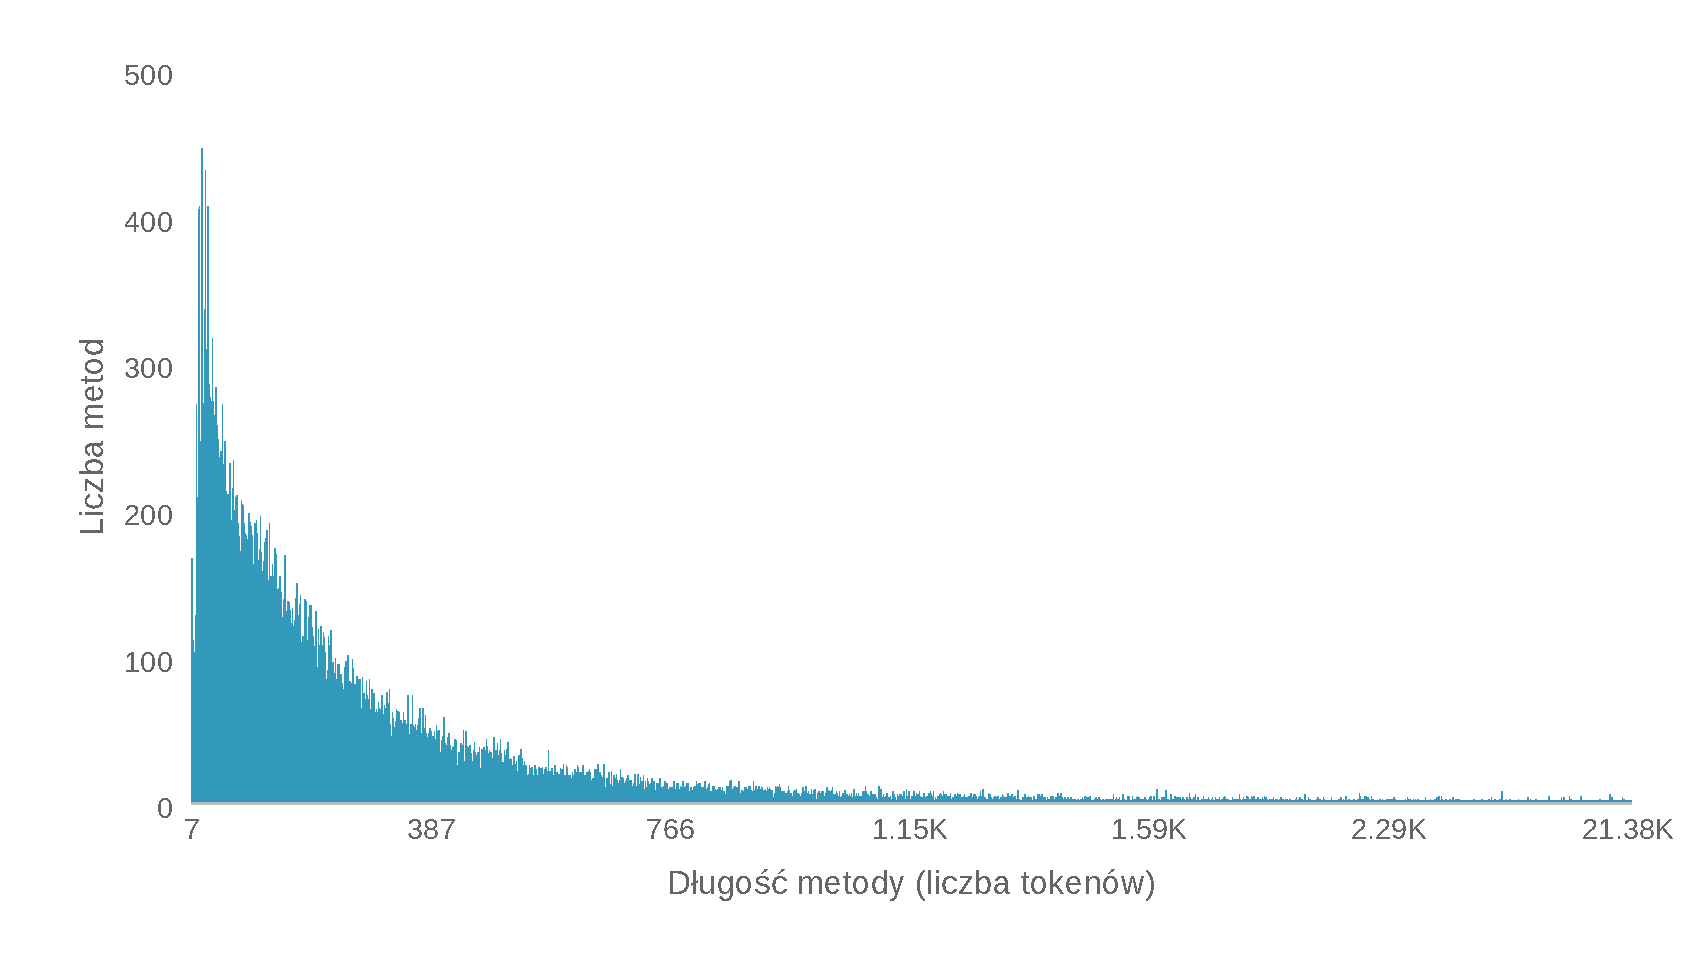
\includegraphics[width=\textwidth]{learn/input-histogram.eps}
\caption{Histogram długości zebranych metod (w tokenach)}
\label{fig:learn:histogram-dlugosci}
\end{figure}

Bez zaskoczenia -- przeważająca większość refaktoryzowanych metod jest krótka -- dużo krótsza od maksymalnej długości. Moda dla zbioru długości metod jest równa 29, mediana -- 168. 
%Te wyniki skłoniły autora rozprawy do~znacznego ograniczenia długości metod podawanych na~wejściu modelu jeszcze przed pierwszą próbą uczenia.

W~przypadku zbyt długich metod zmiany w~nich przeprowadzane dotyczą często tylko jednego z~wielu fragmentów kodu i~nawet jeśli jest poprawiana jego jakość -- w~trakcie uczenia modelu bezwzględnego model będzie źle instruowany o~jakości kodu całej metody. Z~tego powodu postanowiono ograniczyć długość metod, które będą składać się na zbiór treningowy.

Aby znaleźć odpowiednią maksymalną długość metody, do~której powinno zostać ograniczone wejście, przeanalizowano jaka część zbioru danych pozostaje przy jej zmniejszaniu. W~ten sposób oczyszczono zbiór danych z~przykładów, które na~pewno nie prezentują kodu wysokiej jakości oraz -- docelowo -- przyspieszono obliczenia modelu. Tabela \ref{tbl:learn:max-len} przedstawia zależność maksymalnej długości metody od liczby próbek, która pozostaje po nałożeniu takiego ograniczenia. Ostatecznie do~obliczeń przyjęto ograniczenie długości metody do~200 tokenów. To ograniczenie wydaje się już spore, jednakże 200 tokenów w~rozbiorze syntaktycznym metody przekłada się na~około 30-40 linii kodu, co według książki \cite{martin2009clean} oraz autora rozprawy i~tak jest jeszcze zbyt długą metodą.

\begin{table}[h]
\centering
\caption{Liczba próbek pozostałych w~zbiorze danych wejściowych po wprowadzeniu poszczególnych ograniczeń na~maksymalną długość metody}
\label{tbl:learn:max-len}
\begin{tabular}{|p{.3\textwidth}|p{.3\textwidth}|p{.3\textwidth}|}
  \hline 
  \textbf{Maksymalna długość metody} & \textbf{Liczba pozostałych próbek} & \textbf{Część oryginalnego zbioru wejściowego} \\ \hline
  33000 & 60764 & 100\% \\ \hline
  32000 & 60763 & 100\% \\ \hline
  30000 & 60763 & 100\% \\ \hline
  20000 & 60759 & 100\% \\ \hline
  10000 & 60747 & 100\% \\ \hline
  5000 & 60690 & 100\% \\ \hline
  2000 & 60087 & 99\% \\ \hline
  1000 & 57918 & 95\% \\ \hline
  800 & 56397 & 93\% \\ \hline
  700 & 55254 & 91\% \\ \hline
  600 & 53589 & 88\% \\ \hline
  500 & 51358 & 85\% \\ \hline
  400 & 47910 & 79\% \\ \hline
  300 & 42613 & 70\% \\ \hline
  200 & 34204 & 56\% \\ \hline
  100 & 20226 & 33\% \\ \hline
  50 & 10382 & 17\% \\ \hline
\end{tabular} 
\end{table}



\subsection{Zliczanie zmienionych tokenów}

Analizując przypadkowo wybrane przykłady zebranych refaktoryzacji, zwrócono uwagę na~powtarzające się sytuacje, których nie wzięto wcześniej pod uwagę, a~które pojawiały się w~danych wejściowych. Ich jakość byłaby trudna do~rozstrzygnięcia nawet przez programistę bez znajomości dodatkowego kontekstu. Niektóre przykłady to:

\begin{enumerate}
\item metody w~interfejsach, do~których została dodana domyślna implementacja (jest to możliwe od Javy w~wersji 8),
\item przeniesienie implementacji w~górę hierarchii klas -- zastąpienie metody, która dotychczas była abstrakcyjna na~metodę nieabstrakcyjną posiadająca implementację,
\item usunięcie całego ciała metody,
\item wykomentowanie lub usunięcie części kodu w~ciele metody bez zamiany na~np. wywołanie wydzielonej metody prywatnej,
\item dodanie nowego kodu w~ciele metody,
\item minimalna zmiana w~ciele metody, np. zmiana operatora \texttt{<} na~\texttt{<=} w~warunku logicznym.
\end{enumerate}

Odkrycie takich przykładów w~zebranych przykładach refaktoryzacji odsłoniło potrzebę dokładniejszego ich przefiltrowania. 
%Nie wystarczy, jak założono w~sekcji \ref{sec:learn:len-limit}, ograniczyć długości analizowanych metod. 
Oprócz ograniczenia długości metod, należy także sprawdzić czy kod wewnątrz nich rzeczywiście jest \underline{zmieniany}. Należy wykluczyć przypadki, w~których kod jest tylko dodawany bądź usuwany. W~takiej sytuacji nie tylko programista nie byłby w~stanie określić, czy kod po danej zmianie jest czytelniejszy, ale także podawanie takiego przykładu w~trakcie uczenia modelu bezwględnego wprowadza go w~błąd. W~ten sposób przy usuwaniu ciała metody model uczy się, że~metoda bez ciała jest metodą z~kodem wysokiej jakości, a~przy dodaniu implementacji -- odwrotnie.

W celu przygotowania danych, przetworzono raz jeszcze zgromadzone rozbiory syntaktyczne metod i~na czas przetwarzania umieszczono każdy węzeł drzewa w~osobnej linii (zob. skrypt \path{15_prepare_rnn_input_by_diff.php} z~repozytorium \cite{fracz:refactor-extractor}). Następnie porównano tak przygotowane rozbiory syntaktyczne za~pomocą prostej implementacji porównywania zawartości ciągów znaków \texttt{Diff}\footnote{\url{http://code.iamkate.com/php/diff-implementation/}}. Wynikiem takiego porównania jest tablica, z~której każdy element jest parą wartości informującą o~tym co stało się odpowiednio z~danym tokenem przed i~po refaktoryzacji. Informacje te zostały przekazane jako stałe:

\begin{enumerate}
\item \texttt{Diff::UNMODIFIED} jeśli token przed i~po przeprowadzonej zmianie jest niezmieniony,
\item \texttt{Diff::INSERTED}, jeśli token został dodany w~trakcie refaktoryzacji,
\item \texttt{Diff::DELETED}, jeśli token został usunięty w~trakcie refaktoryzacji.
\end{enumerate}

W celu wyeliminowania niejednoznacznych przykładów wymienionych na~początku tej sekcji, ze~zbioru danych wejściowych odrzucono przykłady które w~wyniku porównania nie zwróciły obydwu stałych oznaczających dodanie lub usunięcie danego tokenu. Odfiltrowano w~ten sposób przekształcenia, które tylko dodają bądź tylko usuwają kod z~metody.
 
Ponadto, dla każdej zmiany wyznaczono liczbę zmienionych tokenów, zliczając pary zawierające wartość \texttt{Diff::INSERTED} lub \texttt{Diff::DELETED}.

%\subsection{Dalsze ograniczanie długości analizowanych metod}
%Kolejny raz podjęto decyzję o~ograniczeniu długości metody do~200 tokenów.  Zwrócono bowiem uwagę, że~w~przypadku zbyt długich metod zmiany w~nich przeprowadzane dotyczą często tylko jednego z~wielu fragmentów kodu i~nawet jeśli jest poprawiana jego jakość -- w~trakcie uczenia modelu bezwzględnego model będzie źle instruowany o~całkowitej jakości kodu. To ograniczenie wydaje się już spore, jednakże 200 tokenów w~rozbiorze syntaktycznym metody przekłada się na~około 30-40 linii kodu, co według \cite{martin2009clean} oraz autora rozprawy i~tak jest jeszcze zbyt długą metodą.

%\subsection{Pozbycie się nawiasowania z~rozbioru syntaktycznego}

%W trakcie analizy rozbiorów syntaktycznych metod zwrócono także uwagę, że~nawiasowanie tokenów, które zgodnie z~sekcją \ref{sec:impl:rnn-input} odzwierciedla strukturę kodu źródłowego, zdecydowanie utrudnia analizę danych wejściowych przez człowieka. Spróbowano więc przygotować zbiór danych wejściowych z~pominiętym nawiasowaniem -- czyli traktowaniem rozbioru syntaktycznego metody jako płaskiej listy węzłów, które następując jeden po drugim reprezentują przeanalizowany kod źródłowy. W~ten sposób tracona jest informacja o~strukturze kodu źródłowego -- niemożliwe byłoby odtworzenie kodu na~podstawie tak uproszczonego rozbioru syntaktycznego. Autor rozprawy miał jednak nadzieję, że~w~ten sposób wejście stanie się łatwiej zrozumiałe również dla tworzonego modelu.

%Niestety, próba nauczenia modelu tak przygotowanymi danymi dała rezultaty bliskie losowemu klasyfikatorowi, dlatego ostatecznie pomysł z~uproszczeniem formatu danych wejściowych został porzucony.



\subsection{Decyzje usprawniające przebieg uczenia}
\label{sec:learn:filter-best-result}

Najlepszą kombinacją reguł i~parametrów opisanych w~tej sekcji okazało się:

\begin{itemize}
\item ograniczenie długości metod do~200 tokenów (do 30-40 linii kodu)
\item odfiltrowanie zmian, które wyłącznie dodają lub usuwają kod
\item odfiltrowanie zmian, które zmieniają mniej niż 5 lub więcej niż 100 tokenów w~rozbiorze syntaktycznym
%\item zwiększenie liczby ukrytych jednostek \gls{lstm} z~128 do~256
\end{itemize}






Przyjęcie nowych reguł filtrowania danych wejściowych spowodowało kolejne zmniejszenie ich liczby. Po nałożeniu nowych warunków na~dane wejściowe w~zbiorze pozostaje 9925 zmian refaktoryzacyjnych. Porównując tę liczbę do~liczby wszystkich pozyskanych metod o~długości do~200 tokenów z~tabeli \ref{tbl:learn:max-len} można stwierdzić, że~nowe metody filtrowania odrzuciły niemal $\frac34$ analizowanych dotąd zmian jako niejednoznaczne.



\section{Format danych wejściowych modelu}
\label{sec:impl:rnn-input}

Oczekiwanym formatem danych wejściowych dla rekurencyjnej sieci neuronowej jest sekwencja. Z tego powodu kolejnym krokiem było takie przekształcenie posiadanych rozbiorów syntaktycznych, by można było reprezentować je jako ciągi kolejno następujących po sobie węzłów.

Zbiór tokenów, które mogą zostać zwrócone przez omówiony w~sekcji \ref{sec:impl:ast} parser w~sposób naturalny tworzy alfabet, którym będzie posługiwać się model \gls{scqm} w~trakcie trenowania oraz przy późniejszych klasyfikacjach. Po zliczeniu klas implementujących poszczególne rodzaje węzłów \gls{ast} okazało się, że~rozmiar alfabetu wejściowego jest równy 74. Pełny alfabet wejściowy znajduje się w~pliku \path{java-parser/tokens-java.txt} w~repozytorium \cite{fracz:refactor-extractor}.

Aby zbliżyć istniejącą reprezentację do~sekwencji, zamieniono wcięcia symbolizujące zagnieżdżenie poszczególnych węzłów na~nawiasowanie. W~ten sposób uzyskiwano jeden długi ciąg znaków, w~którym zachowane są wszystkie informacje z~oryginalnego rozbioru syntaktycznego, łącznie ze strukturą kodu źródłowego. Listing \ref{lst:impl:tokens-string} przedstawia przekształcony w~ten sposób rozbiór syntaktyczny z~listingu \ref{lst:impl:example-ast-after}.

\begin{lstlisting}[frame=single,caption={Reprezentacja rozbioru syntaktycznego metody w~postaci ciągu znaków},captionpos=b,label={lst:impl:tokens-string}]
(MethodDeclaration((BlockStmt(ReturnStmt(MethodCallExprNullLiteralExprNameExpr(SimpleName)SimpleName)))ClassOrInterfaceType(SimpleName)SimpleNameMarkerAnnotationExpr(Name)))
\end{lstlisting}

Wprowadzenie nawiasowania wymagało dodania kolejnych dwóch słów do~alfabetu wejściowego: nawiasu otwierającego ,,\texttt{(}'' oraz zamykającego ,,\texttt{)}''. W~rezultacie, liczba możliwych tokenów wzrosła do~76.

Na tym etapie zdecydowano też o~zamianie tokenów składających się na~alfabet wejścia na~liczby w~celu ich łatwiejszej reprezentacji w~kodzie źródłowym modelu. Każdemu tokenowi przypisano liczbę naturalną, będącą numerem linii z~pliku zawierającego alfabet wejściowy (\path{java-parser/tokens-java.txt} w~repozytorium \cite{fracz:refactor-extractor}), przy czym pierwsza linia to 0, druga to 1 itd. W~ten sposób zdefinowano alfabet wejścia jako liczby naturalne od 0 do~75. Na~listingu \ref{lst:impl:tokens-numbers} przedstawiono przekształcony rozbiór syntaktyczny z~listingu \ref{lst:impl:tokens-string}. Liczby, będące tokenami, rozdzielono przecinkami, które służą wyłącznie odseparowaniu kolejnych wyrazów wejścia od siebie. Brak takiej separacji w~poprzedniej reprezentacji rozwiązano za~pomocą zamiany tokenów na~liczby w~malejącym porządku według długości tokenów. W~ten sposób najpierw zamieniono podstring \texttt{NameExpr} a~dopiero potem \texttt{Name}.

\begin{lstlisting}[frame=single,caption={Reprezentacja rozbioru syntaktycznego metody w~postaci sekwencji liczb},captionpos=b,label={lst:impl:tokens-numbers}]
74,56,74,74,20,74,32,74,73,63,36,74,4,75,4,75,75,75,38,74,4,75, 4,60,74,10,75,75,75
\end{lstlisting}

Reprezentacja rozbioru syntaktycznego jako ciągu liczb spowodowała naturalny wybór formatu danych wejściowych dla budowanego modelu -- plików \gls{csv}.

W celu ułatwienia wczytania danych treningowych do docelowej implementacji sieci neuronowej
%wymagania implementacyjne opisane w~sekcji \ref{sec:impl:rnn} powodują konieczność 
podjęto decyzję o~reprezentacji wejścia jako dwuwymiarowej macierzy. Oczywiście, zebranych metod nie cechuje ta sama liczba tokenów. Przed przygotowaniem danych należy więc znaleźć najdłuższą z~nich i~ustalić w~ten sposób pożądany rozmiar każdej sekwencji danych wejściowych. Krótsze metody które mają znaleźć się w~wejściowym zbiorze danych należy dopełnić następnie zerami tak, by liczba tokenów w~każdym wierszu danych była jednakowa. Liczbę znaczących tokenów w~każdej sekwencji wejściowej będzie przekazywana osobno do~sieci neuronowej.

Poza rozbiorami syntaktycznymi i~ich długością, w~trakcie uczenia modelu należy także dostarczyć oczekiwaną klasyfikację danego przykładu. Zgodnie z~projektem (zob. sekcje \ref{sec:proj:bz} oraz \ref{sec:proj:wz}), klasyfikacją przykładu jest para liczb $[P_G,P_B]$, gdzie $P_G$ oznacza prawdopodobieństwo pozytywnej próbki a~$P_B$ -- prawdopodobieństwo negatywnej próbki. W~trakcie uczenia dla każdej sekwencji wejściowej należy przekazać jako oczekiwaną klasyfikację wektor $[1,0]$ dla przykładu pozytywnego i~$[0,1]$ dla przykładu negatywnego.

Aby zminimalizować wpływ sposobu pozyskania danych na~wyniki uczenia, przygotowywane sekwencje były układane w~losowej kolejności. Dzięki temu metody pobrane z~kolejnych projektów nie znajdowały się obok siebie w~macierzy wejściowej.

Dane w~kolejnych etapach uczenia modelu (zob. rozdział \ref{ch:learn}) były przygotowywane za~pomocą skryptów \texttt{10\_*} -- \texttt{15\_*} z~repozytorium \cite{fracz:refactor-extractor}. Gotowe dane wejściowe zostały umieszczone w~katalogu \texttt{input} w~repozytorium \cite{fracz:code-quality-tf}. Poza kilkoma wyjątkami, nazwy katalogów z~danymi wejściowymi były tworzone według reguły \path{M-D-java}, gdzie $M$ to maksymalna długość wiersza wejścia a~$D$ to skrótowy opis metody przygotowania zbioru. Przykładowo \path{200-diff5to100noonlyaddeddel-java} to katalog z~danymi wejściowymi, które dały najlepszy rezultat uczenia obydwu modeli przed wprowadzeniem wiedzy ekspertowej (maksymalna długość metody to 200 tokenów, odrzucono zmiany które wprowadzały mniej niż 5 i~więcej niż 100 zmienionych tokenów, porzucono zmiany które tylko dodawały i~usuwały kod; zob. sekcję \ref{sec:learn:better-ideas}). W~zależności od modelu dla którego zbiór danych był przygotowywany, foldery z~plikami wejściowymi zawierają pliki dla modelu \gls{ascqm} lub \gls{rscqm} (zob. kolejne sekcje \ref{sec:impl:input-ascqm} i~\ref{sec:impl:input-rscqm}).

\subsection{Format danych wejściowych dla modelu aSCQM}
\label{sec:impl:input-ascqm}
Zgodnie z~projektem modelu bezwzględnego \gls{ascqm} (zob. sekcja \ref{sec:proj:bz}), na~wejście powinien on otrzymać kolejno wszystkie metody w~wersji przed i~po refaktoryzacji. W~tym przypadku metody przed zmianą powinny być klasyfikowane jako kod niskiej jakości a~metody po zmianie -- wysokiej.

Zgodnie z~wymaganiami opisanymi wcześniej w~tej sekcji, na~wejście do~uczenia modelu bezwzględnego składają się trzy pliki:

\begin{enumerate}
\item \texttt{input.csv} -- zawiera kolejne sekwencje reprezentujące rozbiory syntaktyczne pozyskanych metod (jedna sekwencja wejściowa zajmuje jedną linię w~pliku),
\item \texttt{lengths.csv} -- zawiera rozdzielone przecinkami długości kolejnych rozbiorów syntaktycznych z~pliku \texttt{input.csv}; zawiera zawsze jeden wiersz danych; liczba elementów w~tym wierszu odpowiada liczbie rozbiorów syntaktycznych (liczbie linii) w~pliku \texttt{input.csv},
\item \texttt{labels.csv} -- oczekiwane klasyfikacje kodu źródłowego z~pliku \path{input.csv}; każda linia w~tym pliku to wektor $[1,0]$ lub $[0,1]$, oznaczający, że~kod, którego rozbiór syntaktyczny jest w~tej samej linii w~pliku \texttt{input.csv} jest odpowiednio wysokiej lub niskiej jakości.
\end{enumerate}

Liczba sekwencji w~pliku \texttt{input.csv} jest zawsze dwukrotnie większa od przedstawianych w~rozprawie liczby analizowanych próbek refaktoryzacji. Wynika to z~faktu, że~w~modelu bezwzględnym każdy przypadek refaktoryzacji daje dwie sekwencje wejściowe -- rozbiór \gls{ast} przed zmianą (przykład negatywny) oraz rozbiór \gls{ast} po zmianie (przykład pozytywny).

\subsection{Format danych wejściowych dla modelu rSCQM}
\label{sec:impl:input-rscqm}

Zgodnie z~opisem modelu względnego \gls{rscqm} w~sekcji \ref{sec:proj:wz}, w~każdej iteracji uczenia wymaga on podania na~wejściu kodu przed i~po wykonanej zmianie. Zakłada się, że~podanie kodu przed refaktoryzacją w~pierwszej kolejności powinno być sklasyfikowane jako pozytywna zmiana (kod poprawia się, gdyż jest poddawany refaktoryzacji). Natomiast podanie w~pierwszej kolejności rozbioru po refaktoryzacji powinno być sklasyfikowane jako przykład negatywny (jakość kodu spada, gdy wprowadzona do~kodu refaktoryzacja jest wycofywana).

Decyzja o~tym, czy daną sekwencję wejściową należy przyjąć tak jak została podana i~potraktować ją jako przykład pozytywny lub czy należy ją odwrócić i~potraktować jako przykład negatywny zostanie podjęta na etapie wczytywania danych do sieci neuronowej, w~trakcie uczenia. Dzięki temu w~kolejnych iteracjach ten sam przykład może być potraktowany na~różne sposoby, prezentując w~odwróconych przypadkach niejako zmianę wycofującą refaktoryzację. To pozwala na przedstawienie modelowi różnych punków widzenia na tę samą próbkę i~pokazania, że nie każda zmiana podnosi jakość kodu -- nawet w~danych treningowych. Z~tego też powodu w~plikach będących wejściem dla modelu względnego nie jest podawana oczekiwana klasyfikacja.

Uwzględniając powyższe wymagania, dane treningowe dla modelu względnego złożone są z~czterech plików:

\begin{enumerate}
\item \texttt{input-before.csv} -- zawiera kolejne sekwencje reprezentujące rozbiory syntaktyczne pozyskanych metod; jedna sekwencja wejściowa zajmuje jedną linię w~pliku; umieszczone tu rozbiory syntaktyczne opisują metody przed wykonaniem refaktoryzacji, czyli próbki o~lepszej jakości kodu,
\item \texttt{lengths-before.csv} -- zawiera rozdzielone przecinkami długości kolejnych rozbiorów syntaktycznych z~pliku \texttt{input-before.csv}; zawiera zawsze jeden wiersz danych; liczba elementów w~tym wierszu odpowiada liczbie rozbiorów syntaktycznych (liczbie linii) w~pliku \path{input-before.csv},
\item \texttt{input-after.csv} -- zawartość analogiczna do~pliku \texttt{input-before.csv}, przy czym zawarte tu rozbiory syntaktyczne opisują metody po wykonaniu refaktoryzacji, czyli próbki o~gorszej jakości kodu; liczba sekwencji wejściowych w~tym pliku jest taka sama jak w~\texttt{input\--before.csv},
\item \texttt{lengths-after.csv} -- zawartość analogiczna do~pliku \path{lengths-before.csv}, przy czym liczby znaczących tokenów dotyczą sekwencji wejściowych z~pliku \texttt{input-after.csv}.
\end{enumerate}

Liczba sekwencji danych w~plikach \texttt{input-*.csv} jest zawsze równa przedstawianej w~rozprawie liczbie analizowanych próbek refaktoryzacji. Wynika to z~faktu, że na jeden przykład analizowany przez model danych składa się zmiana wprowadzona do kodu źródłowego, czyli zarówno sekwencja reprezentująca rozbiór syntaktyczny z~pliku \texttt{input-before.csv} oraz sekwencja z~pliku \texttt{input-after.csv}.

\pagebreak
\section{Podsumowanie}
\label{sec:impl:results}

Jak zaznaczono w~sekcji \ref{sec:impl:wybor-github}, \textbf{350 otwartych projektów z~GitHuba} zostało przeszukanych pod kątem zmian refaktoryzacyjnych. Według zadanych słów kluczowych (zob. Tabela \ref{tbl:impl:keywords}) odnaleziono w~nich \textbf{17967 zmian wykonujących refaktoryzację} kodu źródłowego. Commity te obejmowały zmiany w~\textbf{163013 klasach Javy}. Spośród nich zidentyfikowano 121696 metod, które były modyfikowane podczas znalezionych refaktoryzacji.

Po zastosowaniu bardziej rygorystycznego podejścia w~identyfikacji zmian refaktoryzacyjnych tylko po temacie \textit{commita}, w~danych pozostaje \textbf{60764 metody} (50\% zbioru wyjściowego), w~których potencjalnie udało się zidentyfikować zmiany poprawiające jakość kodu.

Po analizie zebranych próbek podjęto próby usunięcia z~nich szumu danych, nakładając ograniczenia na ich długość oraz liczbę zmienianych tokenów. W~ten sposób na zbiór danych treningowych najlepszego uzyskanego wariantu jakościowego modelu kodu źródłowego składa się \textbf{9925 metod poddanych refaktoryzacji}. 
%Zbudowanie na~ich podstawie rozbiorów syntaktycznych oraz dostarczenie wiedzy ekspertowej na~temat jakości kodu od programistów w~opisanym badaniu pozwoliły stworzyć odpowiedni zbiór danych uczących, dzięki którym możliwe jest zbudowanie jakościowego modelu kodu źródłowego \gls{scqm}.

% Zebranie odpowiedniej ilości mało zaszumionych danych jest jednym z~większych problemów wszystkich wyzwań związanych z~uczeniem maszynowym. Jednakże bez tych czynnoóści nie można liczyć na~zadowalające efekty uczenia.

%W dalszych pracach skupiono się na~skutecznym wytrenowaniu zaimplementowanego modelu za~pomocą zgromadzonych przykładów.

\cleardoublepage
\chapter{Badanie opinii programistów o~jakości kodu}
\label{ch:codefracz}

\begin{addmargin}{1cm}
Uzyskane w~sposób automatyczny próbki kodu o~różnej jakości stanowią solidną bazę wyjściową, która powinna umożliwić przekazanie do jakościowego modelu kodu źródłowego odpowiedniej wiedzy. Jak jednak już podkreślono kilkakrotnie, jakość kodu źródłowego jest niezwykle subiektywnym pojęciem, rozumianym różnie przez różnych programistów. W~celu poprawienia trafności i~zbudowania wiarygodnego zbioru walidacyjnego opracowano i~przeprowadzono i~opisano w~niniejszym rozdziale badanie opinii programistów na temat jakości kodu źródłowego. 
\end{addmargin}

\section{Klasyfikacja przez programistów}
\label{sec:impl:codefracz}

W celu poprawienia jakości danych wejściowych i~w~konsekwencji -- uzyskania lepszej trafności tworzonego modelu jakościowego -- postanowiono przeprowadzić badanie pozwalające sklasyfikować zebrane przykłady refaktoryzacji lepiej niż automatyczne reguły zastosowane podczas gromadzenia danych (zob. sekcję \ref{sec:impl:identification-commits}).

Podstawowym ryzykiem obranej metodyki gromadzenia próbek kodu źródłowego o~różnej jakości jest błędna identyfikacja zmian wprowadzających refaktoryzację. Zaproponowana w~sekcji \ref{sec:impl:identification-commits} metoda wyszukiwania zmian po słowach kluczowych może się czasem nie sprawdzać, a~co za~tym idzie -- dostarczać do~modelu dane, które wprowadzają szum informacyjny lub -- co gorsze -- wprowadzają model w~błąd. Co więcej, te obawy zostały potwierdzone gdy podczas uczenia modelu zidentyfikowano szereg kolejnych problemów w~danych wejściowych takich jak zmiany dotyczące dodawania lub usuwania całego ciała metody lub wykomentowywania całej implementacji (zob. sekcja \ref{sec:learn:better-ideas}). Nawet jeśli poprawnie wybrano \textit{commit} wprowadzający refaktoryzację, nie można być pewnym że~wszystkie zmieniane w~nim metody rzeczywiście podnoszą jakość swojego kodu.

W celu wyeliminowania problematycznych przykładów w~danych wejściowych oraz uzyskania ich poprawnej klasyfikacji, zaprojektowano i~przeprowadzono badanie mające na~celu zebranie od programistów opinii na~temat pojmowania przez nich jakości i~czytelności kodu źródłowego.

\section{Projekt badania}
\label{sec:impl:codefracz-project}
W celu zebrania opinii, zostaje przygotowana specjalna platforma działająca on-line, prezentująca kod przed i~po zmianie. Respondent ma możliwość oceny tej zmiany na~trzy sposoby:

\begin{enumerate}
\item kod przed zmianą jest lepszy,
\item kod po zmianie jest lepszy,
\item jakość kodu w~tej zmianie nie zmienia się.
\end{enumerate}

Każdy przykład zostaje danej osobie przedstawiony tylko jeden raz -- powtórzenia są wykluczane na~poziomie przeglądarki internetowej. Przykłady są podawane użytkownikom w~kolejności losowej. Czas na~udzielenie odpowiedzi jest ograniczony do~60 sekund. Limit ten został ustalony w~oparciu o~kilkanaście klasyfikacji testowych na~etapie projektowania badania wykonanych przez różnych programistów. Po upływie tego czasu przykład klasyfikowany jest jako niezmieniający jakości kodu i~wyświetlana jest kolejna próbka. Nie można też udzielić odpowiedzi szybciej niż po 5 sekundach od zaprezentowania danego przykładu (przeciwdziała to nagminnemu klasyfikowaniu bez zastanowienia).

Aby dany przykład został uznany za~sklasyfikowany, co najmniej 3 osoby muszą podjąć tę samą decyzję na~jego temat. Jeśli przykład zebrał więcej niż 5 głosów i~powyższy warunek nie został spełniony, jest on klasyfikowany jako niezmieniający jakości kodu. Przykłady oznaczone jako sklasyfikowane nie są już przedstawiane kolejnym respondentom.

Eksperyment w~każdej chwili można przerwać i~wrócić do~niego w~dowolnym momencie. Przeglądarka internetowa zapisuje liczbę sklasyfikowanych przez danego użytkownika metod tak, by można było ocenić swój wkład w~budowę modelu \gls{scqm}.

\subsection{Ograniczenie losowych lub nieprzemyślanych opinii}

W celu przeciwdziałania losowym decyzjom udzielanym przez niedoświadczonych lub złośliwych respondentów, wprowadzono dodatkowy mechanizm weryfikacji odpowiedzi. Raz na~kilka/kilkanaście przykładów\footnote{odstęp pomiędzy weryfikacjami był zmienny; każda udzielona klasyfikacja podnosiła prawdopodobieństwo pojawienia się weryfikacji przy następnym pytaniu o~5\%; po udzieleniu poprawnej klasyfikacji prawdopodobieństwo to malało do~zera} osobie biorącej udział w~badaniu przedstawiany jest już jednoznacznie sklasyfikowany przez innych przykład kodu (tzn. wcześniej pojawiły się 3 takie same głosy). Prezentacja tego przykładu nie różni się niczym w~interfejsie użytkownika od takiego, który jeszcze nie został sklasyfikowany. Jeśli respondent podejmie inną decyzję niż poprzednie 3 osoby -- otrzymuje komunikat o~tym, że~platforma stworzona do~badania sprawdziła jego czujność i~niestety test nie został zdany (zob. rysunek \ref{fig:impl:codefracz-warning}). W~ostrzeżeniu jest również informacja o~tym, że~kolejna niezaliczona próba będzie skutkować wykluczeniem danego uczestnika z~eksperymentu na~10 minut. Takie właśnie zachowanie zostało zaimplementowane.

Podobny komunikat otrzyma respondent, który dwa przykłady z~rzędu przekroczy limit czasu przeznaczonego na~odpowiedź. Do~momentu potwierdzenia ostrzeżenia, eksperyment zostanie zatrzymany by przykłady nie klasyfikowały się samoczynnie. W~tym przypadku nie są nakładane żadne kary czasowe. Wyświetlenie komunikatu ma na celu jedynie wstrzymanie wykonywania eksperymentu w~momencie, gdy respondent bez zamknięcia okna przeglądarki z~badaniem odszedł od~stanowiska pracy.

\subsection{Oszacowanie doświadczenia respondentów}

Przy pierwszym udziale w~eksperymencie, platforma wyświetla także formularz wymagający określenia swojego doświadczenia w~programowaniu (zob. rysunek \ref{fig:impl:codefracz-ankieta}). 
% Ta informacja jest kluczowa, gdy pyta się respondentów o~opinię na~temat jakości kodu.

Osoba, która programuje mniej niż 1 rok, prawdopodobnie nie ma jeszcze wykształtowanej opinii na~temat tego, co znaczy ,,czysty'' kod. Z~tego powodu wszystkie głosy od osób, które wybrały ten okres zostały zignorowane na~etapie analizowania zebranych danych. 

Osoba, która w~formularzu zaznaczyła opcję \textit{I'm not a~coder} (z ang. \textit{nie jestem programistą}), po kliknięciu przycisku \textit{Begin!} rozpoczynającego eksperyment była przekierowywana do~strony z~prostą aplikacją do~nauki programowania\footnote{\url{https://www.google.com/doodles/celebrating-50-years-of-kids-coding}}. 

Opcja \textit{I'd rather not say} (z ang. \textit{Nie chcę określać}) została dodana, by respondenci nie czuli się osaczeni przez platformę lub nie odnieśli wrażenia, że~wumusza ona podanie zbyt wielu informacji. Głosy takich osób zostały wzięte pod uwagę.
% przy klasyfikowaniu metod.

Zebrane dane pozwoliły wyciągnąć charakterystykę osób biorących udział w~badaniu. Została ona zaprezentowana na~rysunku \ref{fig:impl:codefracz-respondents-experience}.

\subsection{Próbki kodu poddane analizie w~badaniu}

Metody, które stworzyły zbiór ocenianych w~ramach badania próbek, pochodziły ze~zbioru danych wejściowych, który dał najlepszy rezultat przy uczeniu przed wprowadzeniem wiedzy ekspertowej (zob. sekcja \ref{sec:learn:better-ideas}). Dzięki temu w~większości przypadków można było spodziewać się różnego poziomu jakości pomiędzy prezentowanymi przykładami oraz podobnej realizowanej funkcjonalności. Zbiór ten składał się z~niemal 10 tys. przykładów refaktoryzacji. W~celu klasyfikacji ich wszystkich -- w~najbardziej optymistycznym przypadku wymagałoby to zebrania 30 tys. zgodnych głosów.

Podejrzewano, że~ten wynik jest niemożliwy do~osiągnięcia, dlatego aby nie zostać po badaniu ze~sporą liczbą przykładów sklasyfikowanych tylko przez jedną osobę -- przykłady refaktoryzacji posortowano arbitralnie i~przekazywano do~respondentów przykład wylosowany tylko z~pierwszych 100 metod, które nie zostały jeszcze sklasyfikowane. Po sklasyfikowaniu danego przykładu, został on odrzucany z~puli i~do ,,przesuwającego się okna'' 100 metod dostępnych dla respondentów dochodziła kolejna. To pozwoliło założyć, że~po oddaniu 300 głosów w~zbiorze danych powinno być około 100 sklasyfikowanych metod, zamiast 300 przykładów z~jednym głosem.

\section{Platforma gromadząca opinie o~jakości kodu}

Platformę zaimplementowane zgodnie z~projektem opisanym w~sekcji \ref{sec:impl:codefracz-project}. Wykorzystano do~tego język PHP\footnote{\url{http://www.php.net}} ze~wsparciem \textit{frameworka} Slim\footnote{\url{https://www.slimframework.com}}. Część frontendową aplikacji wykonano za~pomocą Vue.js\footnote{\url{https://vuejs.org}}. Dane zostały zebrane w~bazie danych MariaDB\footnote{\url{https://mariadb.org}}. Całość infrastruktury została skonteneryzowana za~pomocą Dockera\footnote{\url{https://www.docker.com}} i~uruchomiona na~prywatnym serwerze wirtualnym (\gls{vps}).

Na rysunkach \ref{fig:impl:codefracz-front}, \ref{fig:impl:codefracz-ankieta}, \ref{fig:impl:codefracz-codediff} oraz \ref{fig:impl:codefracz-warning} przedstawiono kolejno: stronę główną zapraszającą do~wzięcia udziału w~eksperymencie, wstępną ankietę przed oddaniem pierwszego głosu, ekran prezentujący zmianę w~kodzie poddawaną ocenie oraz komunikat o~oddaniu niepoprawnego głosu dla przypadku weryfikującego poprawność odpowiedzi respondenta.

Interfejs platformy został opracowany w~języku angielskim ze~względu na~udostępnienie platformy publicznie i~zachęcanie do~wzięcia udziału w~eksperymencie również programistów spoza Polski (zob. sekcja \ref{sec:impl:codefracz-respondents}). Ze względu na~powszechność posługiwania się tym językiem wśród programistów, decyzja ta nie utrudniła skorzystania z~platformy również polskojęzycznym respondentom.

Kod źródłowy platformy został umieszczony w~repozytorium \cite{fracz:code-assessor} pod nazwą \textit{Code Assessor}. Platforma była udostępniona pod adresem \url{https://code.fracz.com}. Mimo zakończenia badania do~celów rozprawy, nadal jest uruchomiona i~przyjmuje głosy respondentów, co w~przyszłości być może pozwoli na~powiększenie jakościowego \textit{benchmarku} kodu źródłowego oraz zbudowanie jakościowego modelu, który jeszcze trafniej będzie rozpoznawać czysty kod.

Ciekawym spostrzeżeniem była uwaga od kilku respondentów biorących udział w~jednych z~pierwszych sesji badania, że prezentowanie zmian w~kodzie źródłowym z~domyślnymi kolorami używanymi na ekranie porównywania zmiany (czerwony i~zielony) zbytnio sugerowało, że kod podświetlony na kolor zielony jest kodem wyższej jakości. W~rzeczywistości kolor czerwony oznacza kod usunięty, a~zielony -- dodany w~ramach zmiany. Jednakże w~celu ustosunkowania się do tej (słusznej) uwagi respondentów -- kolory podświetlenia kodu na tym ekranie zostały zmienione na neutralne -- niebieskie (zob. rysunek \ref{fig:impl:codefracz-codediff}).

\begin{figure}
\centering
\includegraphics[width=\textwidth]{impl/codefracz-front.png}
\caption{Strona główna platformy stworzonej do~zebrania opinii o~jakości kodu źródłowego}
\label{fig:impl:codefracz-front}
\end{figure}

\begin{figure}
\centering
\includegraphics[width=0.7\textwidth]{impl/codefracz-ankieta.png}
\caption{Ankieta wyświetlana respondentom badania opinii o~jakości kodu przed oddaniem pierwszego głosu}
\label{fig:impl:codefracz-ankieta}
\end{figure}

\begin{figure}
\centering
\includegraphics[width=\textwidth]{impl/codefracz-codediff.png}
\caption{Ekran pozwalający respondentowi podjąć decyzję o~jakości zaprezentowanej zmiany refaktoryzacyjnej}
\label{fig:impl:codefracz-codediff}
\end{figure}

\begin{figure}
\centering
\includegraphics[width=\textwidth]{impl/codefracz-warning.png}
\caption{Komunikat po wybraniu opinii dla przykładu weryfikującego niezgodnej z~większością oddanych do~tej pory głosów}
\label{fig:impl:codefracz-warning}
\end{figure}

\section{Przebieg eksperymentu}

Dokładniejszego komentarza wymaga rysunek \ref{fig:impl:codefracz-codediff} z~ekranem przedstawiającym analizowaną zmianę i~pozwalającym na~podjęcie decyzji na~temat opinii o~jakości kodu.

Na samej górze przez cały czas trwania eksperymentu wyświetlone jest pytanie, które mu przyświeca, tj. \textit{Which code is better?}, czyli \textit{Który kod jest lepszy?}. Sposób wyboru danych (metody ze~zmian refkatoryzacyjnych) pozwala przypuszczać, że~obydwie zaprezentowane metody realizują podobną odpowiedzialność, ale w~nieco inny sposób. Celowo tutaj nie zadano pytania \textit{Który kod jest wyższej jakości?}, ponieważ celem badania było poznanie ogólnej opinii programistów na~temat tego, \textit{który kod wolą}, lub -- idąc dalej -- \textit{który kod woleliby zaakceptować w~trakcie przeglądu kodu}. Podczas przeglądu kodu programista nie zastanawia się do~końca, który kod ma wyższą jakość, ale który lepiej realizuje powierzone zadanie -- który jest \textit{lepszy}.

Poniżej pytania, główną część ekranu zajmuje zawsze porównywany kod źródłowy wyselekcjonowanych metod. Wykorzystano tutaj ten sam interfejs, jaki stosowany jest przy przeglądach kodu w~portalu GitHub. Początkowo ekran porównania (ang. \textit{diff}) używał standardowych kolorów spotykanych w~platformach do~przeglądu kodu źródłowego -- kolorem czerwonym oznaczano kod który został usunięty w~trakcie zmiany a~kolorem zielonym -- kod, który został dodany. W~trakcie jednej z~pierwszych sesji badania jeden ze~studentów słusznie wskazał, że~takie barwy mogą sugerować odpowiedź na~zadawane pytanie (naturalnie zielony kolor jest raczej ,,lepszy''), dlatego zmieniono kolorystykę na~niebieską tak, by po lewej i~prawej stronie porównania była ona identyczna oraz nie sugerowała jakości kodu.

Warto tutaj zaznaczyć, że~kod po lewej stronie nie zawsze był kodem przed refaktoryzacją a~kod po prawej -- po. Taka sytuacja jest naturalna w~trakcie wykonywania przeglądu kodu. Pomimo że~respondenci nie byli dokładnie zaznajomieni ze~sposobem pozyskania prezentowanych metod, część z~nich mogła założyć że~kod po prawej stronie jest kodem po zmianie, więc jest lepszy. Z~tego powodu opisywany ekran losowo przedstawiał kolejne zmiany, czasem prezentując je tak jak zostały pozyskane ze~zmiany refaktoryzacyjnej, a~czasem na~odwrót -- symulując niejako wycofywanie refaktoryzacji. Takie zachowanie minimalizuje ryzyko pozyskania szumu danych od osób, które mogłyby przyjąć regułę ,,zaznaczam zawsze prawy kod jako lepszy''. W~połączeniu z~metodami próbującymi zidentyfikować osoby klasyfikujące przykłady metod bez zastanowienia (zob. sekcja \ref{sec:impl:codefracz-project}) uzyskano platformę, która wymagała od respondentów rzeczywiście poprawnej klasyfikacji próbek.

Pod wyświetloną próbką kodu do~oceny wyświetlono trzy przyciski. W~lewym dolnym rogu umieszczono zielony przycisk \textit{The left one is better}, \textit{Kod po lewej jest lepszy}. W~prawym dolnym rogu -- analogicznie -- zielony przycisk \textit{The right one is better}, tj. \textit{Kod po prawej jest lepszy}. Na~środku znalazł się pomarańczowy przycisk z~emotikonką \textit{shruga}, dobrze znanej w~środowisku programistów (\shrug), oznaczającą ,,nie wiem'', ,,nie mam pojęcia'' lub ,,nie mam zdania''. Po kliknięciu przycisku, głos respondenta jest zapisywany w~bazie danych, a~ekran porównania pokazuje kolejną próbkę.

Niebieski pasek pod przyciskami ,,napełniał się'' w~miarę upływu czasu, prezentując w~ten sposób ustalony 60-sekundowy limit oczekiwania na~udzielenie odpowiedzi. Gdy limit został osiągnięty, zmiana była klasyfikowana przy użyciu środkowego przycisku (nawet jeśli nie został on wybrany) i~respondent otrzymywał kolejną próbkę do~oceny. Zgodnie z~zaprojektowanymi zasadami opisanymi w~sekcji \ref{sec:impl:codefracz-project}, przez pierwsze 5 sekund respondent nie może dokonać klasyfikacji, co w~interfejsie użytkownika jest zaznaczone wyszarzeniem przycisków tak, by wyglądały one na~nieaktywne.

W prawym górym rogu użytkownik może zdecydować o~sposobie wyświetlania porównania kodu. Może to być sposób \textit{Side by side} (wybrany domyślnie), prezentujący dwie metody po lewej i~prawej. Drugi sposób to \textit{Unified}, prezentujący jeden kod źródłowy, a~usunięte i~dodane linie są oznaczone odpowiednio przez znaki $-$ i~$+$ (ten sposób wyświetlania zmiany jest znany choćby z~linii poleceń i~komendy \texttt{git diff}). Dzięki temu respondent może wybrać widok zmiany do którego jest przyzwyczajony i~maksymalnie skupić się na~prezentowanych przykładach a~nie na~ich formie. Obok przełącznika widoku ekran przedstawia liczbę sklasyfikowanych dotąd metod.

Naśladując styl używania \gls{ide} przez programistów oraz by dostarczyć łatwiejsze w~użytkowaniu narzędzie, opisywaną funkcjonalnością można sterować także przy użyciu klawiatury. Wciskając strzałkę w~lewo, w~prawo bądź na~dół, można sklasyfikować zaprezentowaną próbkę odpowiednio jako ,,lewy kod jest lepszy'', ,,prawy kod jest lepszy'' lub ,,nie wiem''. Klawisz \textit{Esc} przerywa eksperyment i~przenosi użytkownika do~strony wprowadzającej do~badania (rysunek \ref{fig:impl:codefracz-front}). Podpowiedzi sugerujące możliwość wykorzystania omówionych skrótów klawiaturowych zostały zaprezentowane na~ekranie umożliwiającym klasyfikację przykładu bezpośrednio na~przyciskach wykonujących poszczególne akcje.

\section{Czas trwania eksperymentu i~respondenci}
\label{sec:impl:codefracz-respondents}

Badanie trwało 6 miesięcy (styczeń -- czerwiec 2018). Głównymi respondentami byli studenci i~absolwenci studiów Informatyki na~wydziale Informatyki, Elektroniki i~Telekomunikacji, AGH. W~trakcie zajęć z~przedmiotów Technologie Obiektowe oraz Inżynieria Oprogramowania poświęcono 10-15 minut na~udział w~badaniu. Tematem laboratoriów przeprowadzanych w~ramach tych przedmiotów była jakość kodu, dlatego taka aktywność doskonale wpisywała się w~tok zajęć. Studenci przed badaniem zostali poinformowani o~celu gromadzenia danych oraz zostali wprowadzeni do~obsługi platformy w~formie krótkiej prezentacji. W~swoim toku nauczania odbyli już kursy dotyczące programowania zorientowanego obiektowo oraz wzorców projektowych i~refaktoryzacji. Dzięki temu można było oczekiwać, że~mieli już wykształcone własne opinie na~temat jakości i~czytelności kodu źródłowego, co czyniło ich idealnymi kandydatami do~wzięcia udziału w~badaniu.

Dodatkowo, część klasyfikacji udało się zebrać od użytkowników platformy z~zadaniami do~nauki systemu kontroli wersji Git -- \url{https://gitexerecises.fracz.com}. Jest to jeden z~wcześniejszych projektów doktoranta \cite{fracz2015empirical}, który zyskał sporą popularność w~Internecie tak, że~witryna notuje co najmniej kilkadziesiąt unikalnych odwiedzin dziennie. Ze względu na~naturę aplikacji głównymi odbiorcami są programiści, dlatego wstawienie propozycji pomocy autorowi platformy w~jego kolejnym projekcie polegającej na~ocenie kilku przykładów refaktoryzacji wydawało się dobrym pomysłem -- i~rzeczywiście tak było.

Wykres na~rysunku \ref{fig:impl:codefracz-respondents-experience} zawiera zebrane statystyki przedstawiające doświadczenie respondentów na~podstawie ankiety prezentowanej przed przystąpieniem do~badania. Większość osób posiadała co najmniej dwuletnie doświadczenie w~programowaniu. Tabela \ref{tbl:impl:codefracz-respondents} przedstawia natomiast statystyki opinii zebranych za~pomocą opisanej platformy.

\begin{figure}[h]
\centering
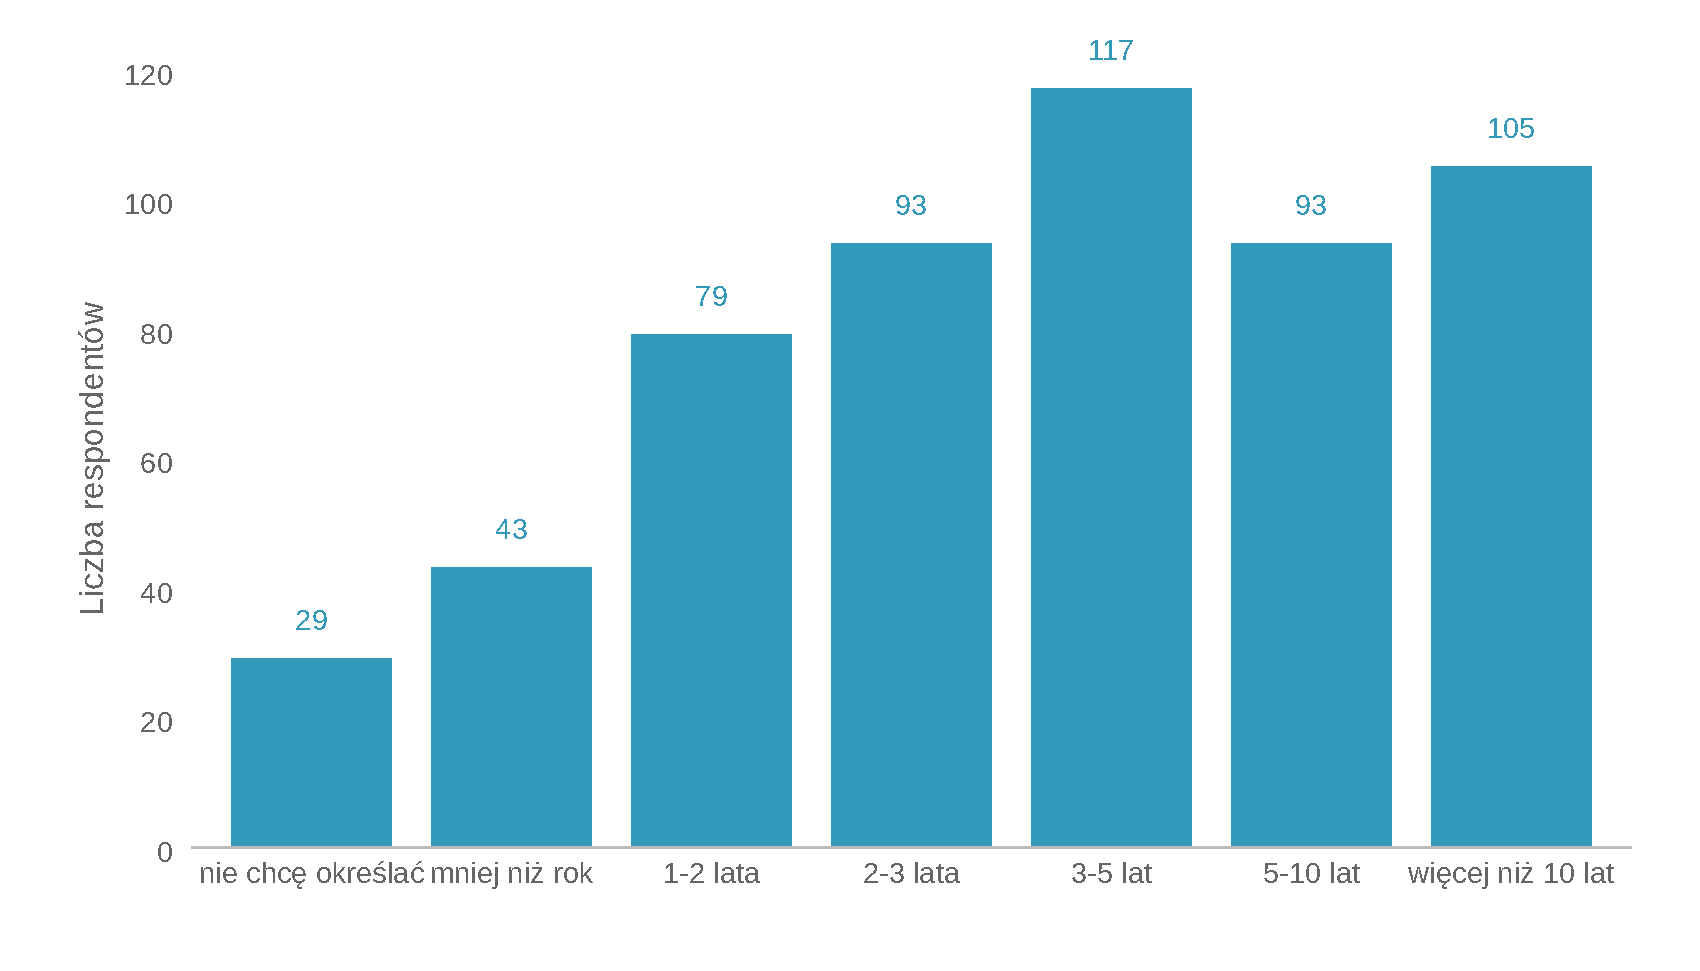
\includegraphics[width=0.7\textwidth]{impl/codefracz-respondents-experience.eps}
\caption{Doświadczenie respondentów, którzy wzięli udział w~badaniu opinii o~jakości kodu źródłowego}
\label{fig:impl:codefracz-respondents-experience}
\end{figure}

\begin{table}[h]
\centering
\caption{Charakterystyka respondentów biorących udział w~badaniu opinii na~temat jakości kodu źródłowego}
\label{tbl:impl:codefracz-respondents}
\begin{tabular}{|l|l|}
  \hline 
  Liczba respondentów & 559 \\ \hline
  Liczba klasyfikacji (głosów) & 5263 \\ \hline
  Średnia liczba głosów / osobę & 9.4 \\ \hline
  Czas konieczny na~podjęcie decyzji (średnia) & 20s \\ \hline
\end{tabular} 
\end{table}

\section{Jakościowy \textit{benchmark} kodu źródłowego}
\label{sec:impl:benchmark}

Ze wszystkich metod sklasyfikowanych przez programistów w~ramach eksperymentu utworzono \textit{benchmark}, tj. zestaw przypadków testowych umożliwiających przetestowanie skuteczności dowolnej metody automatycznie oceniającej jakoś kodu źródłowego w~języku Java. Przykłady z tego zbioru zostały użyte zarówno do uczenia jak i ewaluacji \gls{scqm}.
%Jak wskazano w~dalszej części rozprawy (zob. sekcja \ref{sec:eval:benchmark}), jego część została użyta także do~porównania skuteczności modelu \gls{scqm} z~innymi metodami poddającymi kod statycznej analizie i~metrykami kodu źródłowego. 
% Taki zbiór jest bardzo cennym osiągnięciem i~sporym wkładem w~ten obszar nauki. Benchmark 
% Może być bowiem wykorzystany w~przyszłości do~oceny skuteczności dowolnej metody.
% W~literaturze nie odnaleziono podobnych przykładów benchmarków zawierających kody źródłowe Javy realizujących podobne funkcjonalności, ale o~różnej i~znanej jakości.

Benchmark został umieszczony w~repozytorium \cite{fracz:benchmark}. Zgodnie z~informacjami w~pliku \path{README.md}, katalog \path{src} zawiera 645 przykładów metod o~lepszej i~gorszej jakości, co w~sumie daje 1290 przykładów. Aby kod wewnątrz tych plików był poprawny syntaktycznie, każda sklasyfikowana metoda została opakowana w~deklarację klasy, której nazwa zawiera liczebnik porządkowy przykładu oraz suffix \texttt{Better} dla kodu o~wyższej jakości i~\texttt{Worse} -- dla kodu o~jakości niższej. Ponadto, w~komentarzu nad klasą umieszczono informację z~której próbki z~danych wejściowych pochodzi dany przykład. Wpisano tam także słowo \texttt{before} lub \texttt{after} w~zależności od~tego, czy dany kod w~oryginalnej zmianie był kodem przed czy po zmianie refaktoryzacyjnej.

Listing \ref{lst:impl:benchmark-class} zawiera przykład klasy pochodzącej z~omawianego \textit{benchmarku}.

\begin{lstlisting}[frame=single,caption={Przykładowa klasa wchodząca w~skład jakościowego \textit{benchmarku} kodu źródłowego},captionpos=b,label={lst:impl:benchmark-class}]
// original filename: 00005779.txt
// after
public class Class00000010Better {
    public VirtualFile getProjectFile() {
        if (myProjectFile == null)
            return null;
        return myProjectFile.getVirtualFile();
    }
}
\end{lstlisting}

\section{Podsumowanie}
\label{sec:impl:codefracz-results}

Charakterystyka zebranych odpowiedzi została przedstawiona na~wspomnianej już wcześniej tabeli \ref{tbl:impl:codefracz-respondents}. Natomiast liczba sklasyfikowanych poszczególnych przykładów została przedstawiona w~tabeli \ref{tbl:impl:codefracz-results}.

\begin{table}[h]
\centering
\caption{Uzyskane klasyfikacje w~badaniu opinii o~jakości kodu}
\label{tbl:impl:codefracz-results}
\begin{tabular}{|l|l|}
  \hline 
  Kod przed zmianą jest lepszy & 180 \\ \hline
  Kod po zmianie jest lepszy & 465 \\ \hline
  Zmiana nie wpływa na~jakość kodu & 439 \\ \hline
\end{tabular} 
\end{table}

Ciekawym spostrzeżeniem jest fakt, że~znaczna część zmian refaktoryzacyjnych została sklasyfikowana jako ,,anty-refaktoryzacje''. Niemal połowa z~przeanalizowanych przez uczestników badania przykładów została odrzucona jako niezmieniające jakości. Większość z~nich -- zgodnie z~oczekiwaniami -- została sklasyfikowana jako ,,kod po zmianie jest lepszy''.

Dzięki badaniu uzyskano zbiór \textbf{645 metod, których jakość została sklasyfikowana przez programistów}. Za~ich pomocą został stworzony wzorcowy zbiór treningowy oraz testowy, który następnie wykorzystano w~trakcie uczenia i~ewaluacji modelu \gls{scqm}.


\cleardoublepage
\chapter{Uczenie SCQM}
\label{ch:learn}

\begin{addmargin}{1cm}
%Kolejnym krokiem w~dążeniu do~weryfikacji tezy rozprawy jest przekazanie wiedzy zawartej w~danych zebranych zgodnie z~opisem w~rozdziale \ref{ch:impl} do~modelu sieci neuronowej zaproponowanego w~sekcji \ref{sec:impl:rnn}. Oczywiście, mimo szczerych chęci, tworzony model \gls{scqm} nie dawał od razu zadowalających wyników. W~tym rozdziale opisano kolejne próby poprawiania założonego modelu oraz pomysły na~przygotowanie danych wejściowych, które w~konsekwencji doprowadziły do~oczekiwanego rezultatu.
Zgromadzony zbiór danych wejściowych złożony z~próbek kodu źródłowego o~różnej jakości pozwolił na rozpoczęcie prac nad samym modelem. W~tym rozdziale opisano projekt i~implementację jakościowego modelu źródłowego opartego o~dwukierunkową rekurencyjną sieć neuronową oraz przybliżono przebieg jej trenowania, wraz z~przedstawieniem najlepszego rezultatu na zbiorze testowym. 
\end{addmargin}

\section{Implementacja sieci neuronowej}
\label{sec:impl:rnn}

W sekcji \ref{sec:proj:rnn} przedstawiono motywację stojącą za~wyborem modelu opartego o~dwukierunkową rekurencyjną sieć neuronową z~komórkami \gls{lstm}.

W celu dostarczenia implementacji sieci neuronowej wykorzystano \textit{framework} TensorFlow \cite{tf}. Jest to implementacja różnych metod uczenia maszynowego w~języku Python\footnote{\url{https://www.python.org}} na~wystarczająco wysokim poziomie abstrakcji, by osoba niebędąca specjalistą w~tej dziedzinie mogła wykorzystać ich potencjał.

Kod źródłowy dla modeli \gls{ascqm} oraz \gls{rscqm} znajduje sie odpowiednio w~plikach \texttt{model2.py} oraz \texttt{model4.py} w~repozytorium \cite{fracz:code-quality-tf}. Szczegóły przedstawionych implementacji zostały umieszczone w~dodatku \ref{apdx:scqm-impl}.

Obydwa skrypty pozwalają na uruchomienie ich w~dwóch trybach -- trenowania oraz klasyfikacji. W~trakcie trenowania możliwe jest przekazanie do skryptu zadanego zbioru danych treningowych, pożądanej liczby iteracji, liczby ukrytych jednostek \gls{lstm} oraz innych parametrów pracy sieci neuronowej. Jeżeli skrypt uruchamiany jest w~trybie klasyfikacji, wymaga on podania ścieżki do wytrenowanego wcześniej modelu.

Na początku każdej implementacji znajduje się kod odpowiedzialny za~wczytanie wejścia sieci neuronowej. Dane te, w~zależności od skryptu, posiadają opisany wcześniej format (zob. sekcja \ref{sec:impl:rnn-input}). Następnie budowane są struktury dwukierunkowej rekurencyjnej sieci neuronowej za~pomocą konstrukcji dostarczanych przez narzędzie TensorFlow. W~końcowej części skryptu uruchamiana jest sesja TensorFlow, która wykorzystuje sieć neuronową budując, lub wykorzystując zbudowany wcześniej jakościowy model kodu źródłowego.

\section{Rozmiar zbioru testowego}

Obie implementacje modelu -- względna i~bezwzględna -- każdy zbiór sekwencji wejściowych dzielą w~stosunku $85\%:15\%$. Większy zbiór stawał się danymi uczącymi (treningowymi). Drugi zaś -- danymi testowymi, które nie brały udziału w~uczeniu. 

Wszystkie trafności przedstawione w~rozprawie zostały oparte o~wyniki dla zbioru testowego.

\section{Wykorzystane zasoby obliczeniowe}

Uczenie jakościowego modelu kodu źródłowego na~podstawie zebranych danych nie byłoby możliwe, gdyby nie zasoby obliczeniowe posiadane przez AGH. Teoretycznie model mógłby być obliczony na~sprzęcie domowym (według szacunków trwałoby to około 3-4 tygodni). Jednakże mnogość prób i~różnych konfiguracji, które zostały podjęte podczas uczenia (por. np. tabele \ref{tbl:learn:results-map-wz} i~\ref{tbl:learn:results-map-bz}) musiałaby być w~znaczny sposób ograniczona, co z~pewnością odbiłoby się na~skuteczności uzyskanego modelu jakościowego.

Dzięki superkomputerowi Prometheus AGH udostępnianemu przez Cyfronet i~portal PLGrid\footnote{\url{http://www.plgrid.pl}} oraz wsparciu \gls{gpu} możliwe było skrócenie czasu obliczeń jednej konfiguracji do~około 8 godzin dla modelu \gls{ascqm} oraz około 12 godzin dla modelu \gls{rscqm} (czasy były oczywiście zależne od zadanych parametrów modelu oraz rozmiaru danych wejściowych). Taki czas oczekiwania na~wyniki umożliwił eksperymentowanie z~konfiguracją sieci neuronowej i~uzyskanie najlepszych możliwych wyników.

%Obliczenia zostały wykonane w~ramach grantu \texttt{scqfracz}.

W repozytorium \cite{fracz:code-quality-tf} można odnaleźć skrypty używane do~zlecania zadań obliczeń w~trybie wsadowym (pliki \texttt{batch*.sh}). Wykorzystują one parametry skryptów uczących poszczególne modele (zob. dodatek \ref{apdx:scqm-impl} oraz listingi \ref{lst:learn:learn-ascqm-1} i~\ref{lst:learn:learn-ascqm-2}). Ponadto, poza konfiguracją samego zadania wynikającą z~dostarczonej dokumentacji \cite{cyfronet:prometheus-podstawy}, można z~nich także odczytać użyte w~trakcie obliczeń dodatkowe moduły. Są to:

\begin{enumerate}
    \item \texttt{plgrid/apps/cuda/8.0}\footnote{\url{https://apps.plgrid.pl/module/plgrid/apps/cuda/8.0.61}} -- dostarcza biblioteki umożliwiające wykorzystanie procesorów graficznych \gls{gpu} na~klastrze Prometheus w~architekturze \gls{cuda}\footnote{\url{https://www.nvidia.pl/object/cuda-parallel-computing-pl.html}}
    \item \texttt{plgrid/tools/python/3.6.0}\footnote{\url{https://apps.plgrid.pl/module/plgrid/tools/python}} -- umożliwia korzystanie z~języka Python, w~którym zaimplementowany jest użyty \textit{framework} TensorFlow
\end{enumerate}

Po uprzedniej konfiguracji odpowiednich nazw katalogów zawierających dane użyte do~kolejnych etapów uczenia modelu wewnątrz skryptów wsadowych (wszystkie dane wejściowe wraz z~uzyskanymi wynikami są zamieszczone w~repozytorium \cite{fracz:code-quality-tf}), zadania były zlecane przy użyciu polecenia \texttt{sbatch}. Dzięki trybowi wsadowemu możliwe było obliczanie kilku konfiguracji jednocześnie, a~przy długo trwających obliczeniach możliwe było opuszczenie maszyny i~powrócenie do~wyników uczenia w~późniejszym czasie. Ze~szczegółowymi informacjami na~temat wspomnianej komendy można zapoznać się bezpośrednio z~dokumentacji klastra \cite{cyfronet:prometheus-podstawy}.
%Przykładowa komenda zlecająca zadanie została przedstawiona na~listingu \ref{lst:learn:sbatch}.

%\begin{lstlisting}[frame=single,caption={Komenda \texttt{sbatch} zlecająca obliczenie ustawionej konfiguracji uczenia modelu \gls{rscqm} na~klastrze Prometheus},captionpos=b,label={lst:learn:sbatch}]
%sbatch batch-rscqm.sh
%\end{lstlisting}

Każda sesja uczenia pozostawiała za~sobą dwa artefakty:

\begin{enumerate}
    \item Plik z~rozszerzeniem \texttt{.log} zawierający informacje o~trafności i~błędzie podczas uczenia (na ich podstawie zaprezentowano w~rozprawie wykresy przebiegów uczenia w~kolejnych próbach). Wszystkie pliki z~logami zostały umieszczone w~katalogu \texttt{logs} w~repozytorium \cite{fracz:code-quality-tf}.
    \item Zapisany stan sieci neuronowej na~zakończenie uczenia. Pliki te umożliwiają późniejsze zaimportowanie nauczonego modelu i~użycie go do~sklasyfikowania kolejnych przykładów lub dalszego douczenia. Funkcjonalność ta zostanie wykorzystana przy ewaluacji stworzonego rozwiązania (zob. rozdział \ref{ch:eval}). Ze~względu na~duży rozmiar plików, w~repozytorium nie udostępniono wszystkich wytrenowanych modeli. W~repozytorium \cite{fracz:scqm} znajduje się model, który dał najlepsze rezultaty.
\end{enumerate}

\section{Trenowanie za~pomocą danych zgromadzonych automatycznie}

%\subsection{Zmiana parametrów sieci neuronowej}

%W kolejnych próbach uczenia modelu próbowano także zmieniać konfigurację sieci neuronowej zaproponowaną w~sekcji \ref{sec:impl:rnn}.

%Jedynym parametrem, który spowodował, że~odnotowano zmiany w~wynikach uczenia (przy użyciu tych samych danych), była liczba ukrytych jednostek \gls{lstm}. Liczba ta w~teorii reprezentuje liczbę aspektów, które model jest w~stanie wykryć w~analizowanych danych. Ile jest aspektów, po których można rozpoznać kod wysokiej jakości? Początkowo wybrano arbitralnie liczbę 128, jednak próba uczenia z~większą liczbą ukrytych jednostek pokazała, że~model zachowuje się lepiej po zwiększeniu tego parametru.

Próbki kodu źródłowego metod klas zgromadzone i~przygotowane zgodnie z~opisem w~rozdziale \ref{ch:impl} zostały już wstępnie przefiltrowane. Nałożone ograniczenia mające na celu usunięcie szumu z~danych treningowych (zob. sekcja \ref{sec:learn:better-ideas}) pozwoliły przypuszczać, że~posiadane rozbiory syntaktyczne metod zawierają całkiem sensowne refaktoryzacje.

Na tym etapie wykonano szereg prób uczenia modelu, manipulując sposobem filtrowania danych wejściowych oraz parametrami sieci neuronowej. Jedynym parametrem, który spowodował, że~odnotowano zmiany w~wynikach uczenia (przy użyciu tych samych danych), była liczba ukrytych jednostek \gls{lstm}. Liczba ta w~teorii reprezentuje liczbę aspektów, które model jest w~stanie wykryć w~analizowanych danych. Ile jest aspektów, po których można rozpoznać kod wysokiej jakości? Początkowo wybrano arbitralnie liczbę 128, jednak próba uczenia z~większą liczbą ukrytych jednostek pokazała, że~model zachowuje się lepiej po zwiększeniu tego parametru.

Tabele \ref{tbl:learn:results-map-wz} i~\ref{tbl:learn:results-map-bz} przedstawiają końcową trafność dla zbioru testowego osiąganą po 50 tys. iteracji dla modelu bezwzględnego i~względnego dla poszczególnych prób kombinacji parametrów i~metody filtrowania danych treningowych.

\begin{table}[H]
\centering
\caption{Trafność modelu dla zbioru testowego przy różnych konfiguracjach po 50 tys. iteracji -- model bezwzględny \gls{ascqm}}
\label{tbl:learn:results-map-wz}
\begin{tabular}{|p{.15\textwidth}|p{.2\textwidth}|p{.2\textwidth}|p{.15\textwidth}|p{.15\textwidth}|}
  \hline 
   \textbf{Maks. długość metody} & \textbf{Min. liczba zmienionych tokenów} & \textbf{Maks. liczba zmienionych tokenów} & \textbf{Liczba jednostek LSTM} & \textbf{Trafność} \\ \hline 
  300 & - & - & 128 & 53\% \\ \hline 
  200 & 10 & - & 128 & 54\% \\ \hline
  100 & 10 & - & 128 & 50\% \\ \hline
  100 & 10 & - & 256 & 53\% \\ \hline
  100 & 10 & 50 & 256 & 56\% \\ \hline
  200 & 10 & 50 & 256 & 54\% \\ \hline
  200 & 10 & 100 & 256 & \textbf{56\%} \\ \hline
\end{tabular} 
\end{table}

\begin{table}[h]
\centering
\caption{Trafność modelu dla zbioru testowego przy różnych konfiguracjach po 50 tys. iteracji -- model względny \gls{rscqm}}
\label{tbl:learn:results-map-bz}
\begin{tabular}{|p{.15\textwidth}|p{.2\textwidth}|p{.2\textwidth}|p{.15\textwidth}|p{.15\textwidth}|}
  \hline 
  \textbf{Maks. długość metody} & \textbf{Min. liczba zmienionych tokenów} & \textbf{Maks. liczba zmienionych tokenów} & \textbf{Liczba jednostek LSTM} & \textbf{Trafność} \\ \hline 
  300 & - & - & 128 & 53\% \\ \hline 
  200 & 10 & - & 128 & 54\% \\ \hline
  100 & 10 & - & 128 & 58\% \\ \hline
  100 & 10 & - & 256 & 59\% \\ \hline
  100 & 10 & - & 512 & 58\% \\ \hline
  100 & 5 & 100 & 256 & 59\% \\ \hline
  100 & 5 & 100 & 256 & 60\% \\ \hline
  100 & 10 & 50 & 256 & 62\% \\ \hline
  200 & 10 & 50 & 256 & 55\% \\ \hline
  200 & 10 & 100 & 256 & 63\% \\ \hline
  200 & 5 & 100 & 256 & \textbf{64\%} \\ \hline
  300 & 5 & 100 & 256 & 62\% \\ \hline
\end{tabular} 
\end{table}

Rezultat uczenia modelu za~pomocą danych zgromadzonych i~przygotowanych zgodnie z~opisem w~rozdziale \ref{ch:impl} i~dla najlepszej uzyskanej konfiguracji parametrów sieci neuronowej przedstawiono na~rysunku \ref{fig:learn:diffacc}.

\begin{figure}[h]
\centering
\includegraphics[width=\textwidth]{learn/diffacc.eps}
\caption{Przebieg trenowania modelu za~pomocą danych zgromadzonych automatycznie}
\label{fig:learn:diffacc}
\end{figure}

Uzyskano trafność modelu względnego \gls{rscqm} na poziomie 64\% i~bezwzględnego \gls{ascqm} na poziomie 56\%. Model prezentuje wyższą trafność niż losowy klasyfikator, jednakże wyniki na tym etapie nie są jeszcze zadowalające. Znaczna różnica pomiędzy osiąganymi trafnościami modelu dla różnych metod filtrowania danych treningowych pokazuje, że~w~pozyskanych automatycznie próbkach rzeczywiście znajduje się sporo szumu danych.

Przed kolejnymi próbami uczenia postawiono także sprawdzić, czy implementacja sieci neuronowej jest zbudowana poprawnie i~czy jest w~stanie przyjąć jakąkolwiek wiedzę z~tak przygotowanych danych treningowych. Przygotowano trzy proste metryki klasyfikowania jakości kodu i~z powodzeniem podjęto próbę przekazania wiedzy o~nich do jakościowego modelu kodu źródłowego. Szczegóły tej ewaluacji zamieszczono w~dodatku \ref{apdx:testing}.


\section{Trenowanie za~pomocą próbek sklasyfikowanych przez programistów}
\label{sec:learn:expert}

Trafność 64\% w~rozpoznawaniu zmiany podnoszącej jakość kodu źródłowego dla modelu \gls{rscqm} jest lepsza niż trafność losowej klasyfikacji. Niemniej jednak, nie można jeszcze na~tym etapie mówić o~sukcesie prezentowanego modelu. Kolejnym krokiem usprawnienia modelu było więc wykorzystanie wiedzy zebranej przy użyciu badania opisanego w rozdziale \ref{ch:codefracz}.

Ważną korzyścią płynącą z~faktu posiadania zbioru poprawnie sklasyfikowanych metod i~ich jakości była możliwość zbudowania pewnego zbioru danych testowych nieposiadających szumu. Trafność obliczana na~jego podstawie może być rzeczywiście traktowana jako podobieństwo działania zaprojektowanego modelu jakościowego do~decyzji podejmowanych przez programistę w~trakcie przeglądu. Zbiór testowy -- podobnie jak poprzednio -- stworzono wybierając losowo 15\% próbek z~pozyskanych danych, co dało 96 metod ocenionych przez programistów, które nie zostały wzięte pod uwagę w~dalszym uczeniu (por. Tabela \ref{tbl:impl:codefracz-results}). Również model nauczony w~oparciu o~reguły z~sekcji \ref{sec:learn:better-ideas} wykazuje dla tak skonstruowanego zbioru testowego wyższą trafność (zob. trafność osiąganą w~początkowych iteracjach na~rysunku \ref{fig:learn:best-mix}).

Przed stworzeniem modelu w~oparciu o~obydwa zestawy danych (to podejście opisano w~sekcji \ref{sec:learn:best-mix}), pierwszą próbą było nauczenie modelu tylko przy użyciu zmian sklasyfikowanych przez programistów jako zmieniających jakość kodu. Tak zbudowany model powinien rzeczywiście posiąść przekazaną w~platformie wiedzę na~temat jakości kodu.

Przebieg uczenia zaprezentowano na~rysunku \ref{fig:learn:expert}. Model bezwzględny \gls{ascqm} nie poprawił się znacząco w~stosunku do~poprzedniego wyniku po dokładniejszym przefiltrowaniu danych wejściowych. Zdecydowaną poprawę widać jednak w~modelu względnym \gls{rscqm}. Dla tak zadanych danych wejściowych osiąga on trafność rozpoznawania zmiany poprawiającej jakość kodu na~poziomie 78\%.

\begin{figure}[h!]
\centering
\includegraphics[width=\textwidth]{learn/expert-only.eps}
\caption{Przebieg uczenia modelu przy danych treningowych zbudowanych na~podstawie metod sklasyfikowanych przez programistów}
\label{fig:learn:expert}
\end{figure}

\section{Najlepszy uzyskany rezultat trenowania modelu}
\label{sec:learn:best-mix}

Ze względu na~niewielką liczbę metod sklasyfikowanych przez programistów (zob. Tabela \ref{tbl:impl:codefracz-results}) sieć neuronowa zbyt dobrze dopasowywała się do~danych treningowych. Przeuczanie się modelu widać także po szybkim osiągnięciu wysokiej trafności dla modelu \gls{rscqm}. To spostrzeżenie doprowadziło do~pomysłu połączenia rozwiązań opisanych w~poprzednich sekcjach \ref{sec:learn:better-ideas} oraz \ref{sec:learn:expert}. W~tym wariancie sieć neuronowa jest uczona początkowo za~pomocą danych treningowych, które nie zostały sklasyfikowane przez programistów ze~względu na~ograniczenia eksperymentu.

Pozostając przy dotychczasowym limicie 50 tys. iteracji uczenia ustalono, że~model będzie uczony przez 80\% z~nich (40 tys.) za~pomocą rozbiorów syntaktyczynch metod pozyskanych za~pomocą ustalonych reguł opisanych w~sekcji \ref{sec:learn:better-ideas}. Następnie, przez kolejne 20\% iteracji (10 tys.), sieć neuronowa zostanie ,,douczona'' poprawnie sklasyfikowanymi metodami przez programistów.

Takie podejście powinno pozostawić w~modelu wiedzę o~jakości kodu źródłowego wyciągniętą bezpośrednio z~otwartych projektów oraz doprecyzować ją za~pomocą pozyskanej opinii programistów o~jakości kodu źródłowego.

Przebieg uczenia zaprezentowano na~rysunku \ref{fig:learn:best-mix}. W momencie wprowadzenia do danych treningowych próbek sklasyfikowanych przez programistów następuje zauważalny wzrost trafności klasyfikacji modelu.

\begin{figure}[h!]
\centering
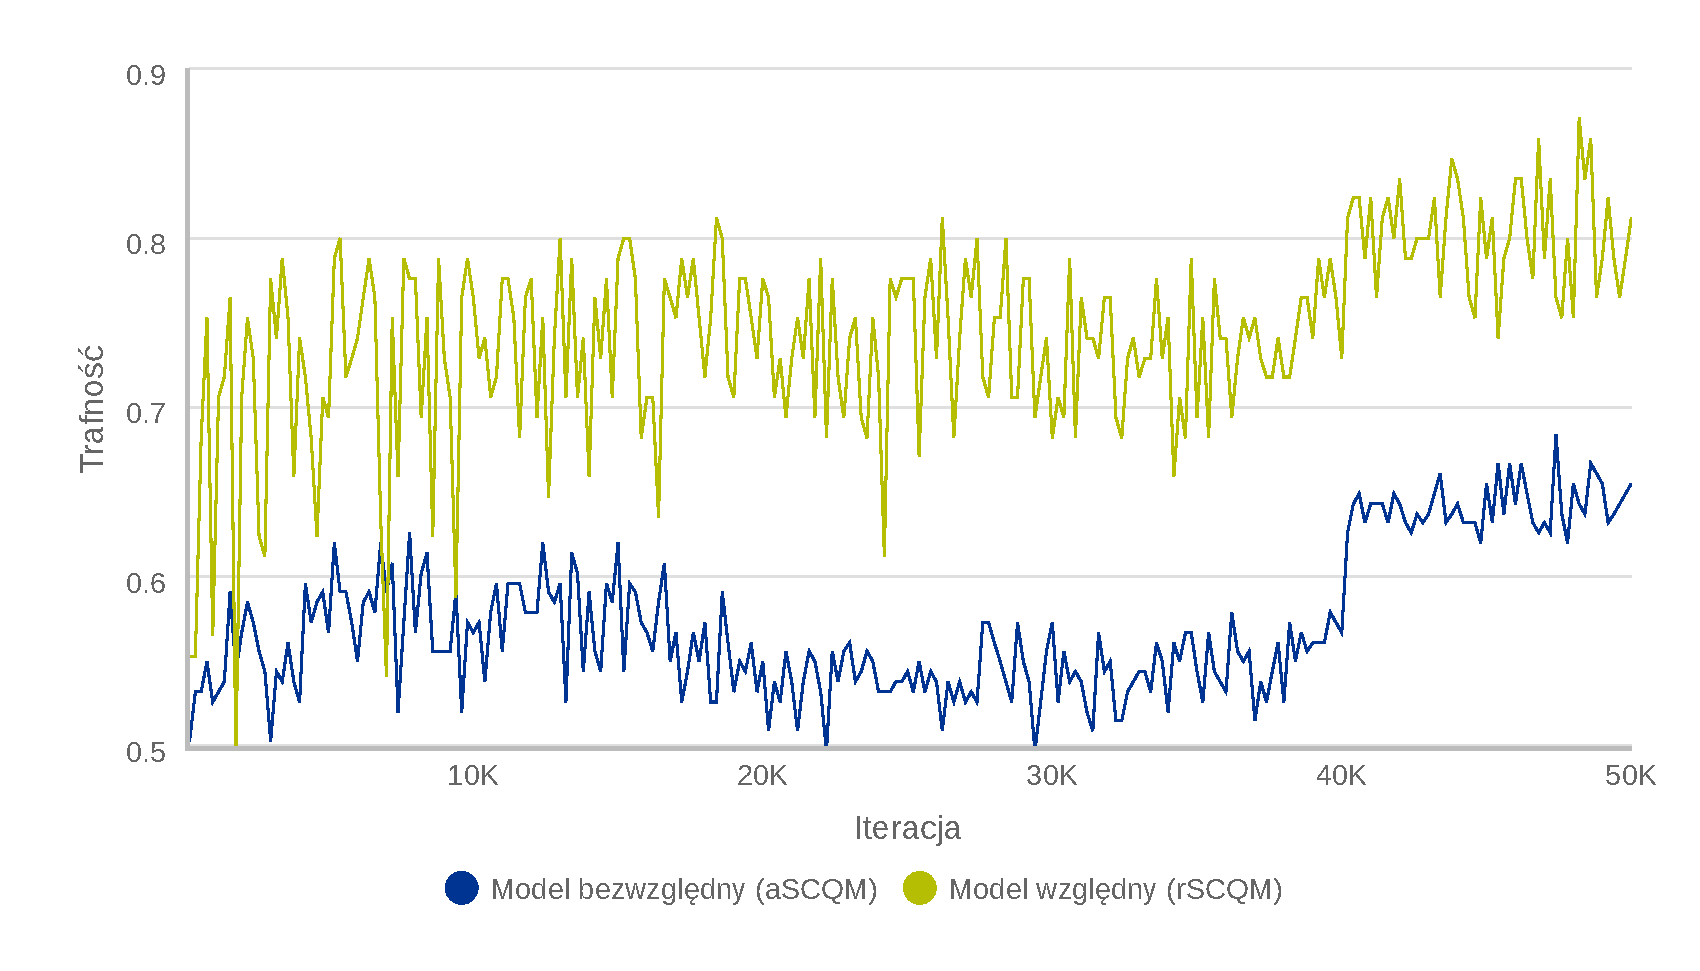
\includegraphics[width=\textwidth]{learn/bestmix.eps}
\caption{Przebieg uczenia modelu przy danych treningowych zbudowanych na~podstawie metod wybranych automatycznie (40 tys. iteracji) oraz metod sklasyfikowanych przez programistów (10 tys. kolejnych iteracji)}
\label{fig:learn:best-mix}
\end{figure}

\pagebreak

\section{Podsumowanie}

Kolejne próby uczenia zaprojektowanego jakościowego modelu kodu źródłowego opisane w~tym rozdziale pozwoliły na~uzyskanie zadowalających rezultatów, a~w~konsekwencji na~kontynuowanie prac nad rozprawą. Proces ten był najbardziej czasochłonną czynnością w~ramach rozprawy ze~względu na~czas oczekiwania na~uzyskanie kolejnych wyników oraz mnogość możliwych rozwiązań.

Na tym etapie uzyskano \textbf{trafność dla modelu \gls{ascqm} na~poziomie 65\%} oraz \textbf{trafność dla modelu \gls{rscqm} na~poziomie 80\%}. Uznano, że~taka trafność uzyskana dla metod sklasyfikowanych w~ramach platformy jest wystarczająca, by podjąć próbę porównania stworzonego modelu z~istniejącymi narzędziami oceniającymi kod, opartymi o~statyczną analizę.

\cleardoublepage
\chapter{Ewaluacja SCQM}
\label{ch:eval}

\begin{addmargin}{1cm}
Trafność uzyskana w~procesie uczenia modelu \gls{scqm} opisana w~poprzednim rozdziale skłoniła autora rozprawy do~podjęcia próby porównania skuteczności stworzonego modelu i~dostępnych obecnie metod, które do~oceny jego jakości wykorzystują statyczną analizę. 
%Pierwszym krokiem prowadzącym do~osiągnięcia tego celu, a~zarazem głównego celu rozprawy, było odpowiednie dostosowanie wytrenowanego modelu we~\textit{frameworku} TensorFlow tak, by mógł on przyjąć dowolny kod źródłowy od użytkownika. 
W tym celu wybrano istniejące jakościowe metryki kodu źródłowego oraz popularne narzędzie klasyfikujące kod pod względem jego jakości: Checkstyle. Porównano ich skuteczność ze~stworzonym modelem, a~wyniki tego porównania zostały opisane w~tym rozdziale. W~ramach ewaluacji wykorzystano wybrane metody z~jakościowego \textit{benchmarku} kodu źródłowego stworzonego w~ramach pracy nad rozprawą.
\end{addmargin}

\section{Narzędzia i~metryki poddane analizie porównawczej}
\label{sec:eval:others}

Rozprawa zakłada wykazanie, że~stworzony jakościowy model kodu źródłowego wykazuje większą trafność w~rozpoznawaniu kodu niskiej jakości niż dostępne obecnie narzędzia wykorzystujące jego statyczną analizę. Jednym z~najpopularniejszych narzędzi powszechnie używanych do~wykrywania zapachów w~kodzie źródłowym w~języku Java jest Checkstyle\footnote{\url{http://checkstyle.sourceforge.net/}}. Porównanie rezultatów osiąganych przez to narzędzie oraz przez model \gls{scqm} jest więc niezbędne do~stwierdzenia użyteczności powstałego rozwiązania w~środowisku produkcyjnym.

Oprócz porównania modelu \gls{scqm} do~wspomnianego narzędzia, wartościowe będzie także porównanie klasyfikacji otrzymywanych z~nowego modelu do~wartości jakościowych metryk kodu źródłowego, które są często wykorzystywane do~automatycznego określania jakości kodu źródłowego. Zgodnie z~opisem w~sekcji \ref{sec:related:metrics} najlepszą skuteczność w~wykrywaniu kodu źródłowego niskiej jakości ma złożoność cyklomatyczna. Nie można więc było jej pominąć w~ewaluacji stworzonego modelu, by wykazać, że~jest on rzeczywiście lepszy od istniejących rozwiązań.

Podobną metryką jest złożoność NPath (ang. \textit{NPath complexity}). Jest to metryka, która określa możliwą liczbę różnych, acyklicznych ścieżek przejścia przez dany kod źrodłowy \cite{nejmeh1988npath}. Podobnie jak przy złożoności cyklomatycznej, wyższa wartość metryki oznacza bardziej skomplikowany kod.

Kolejną metryką, do~której autor rozprawy postanowił porównać predykcje \gls{scqm} jest metryka NCSS (ang. \textit{Non Commenting Source Statements}, wyrażenia w~kodzie źródłowym niebędące komentarzami). Metryka ta zlicza wyrażenia w~kodzie źródłowym, które nie są komentarzami ani pustymi blokami kodu. Jej wartość więc można rozumieć jako liczbę operacji wykonywanych w~zadanym kodzie źródłowym. Jak zasugerowano w~\cite{ayewah2007evaluating}, NCSS jest nieco bardziej wyszukanym określeniem rozmiaru kodu aniżeli liczba jego linii. Pomimo prostoty tej metryki, NCSS jest często zawierana w~domyślnych konfiguracjach sprawdzeń dla narzędzia Checkstyle -- a~co za~tym idzie -- często jej wyniki są brane pod uwagę w~środowiskach produkcyjnych. Podobnie jak w~poprzednich metrykach -- wyższa wartość oznacza kod niższej jakości.

Próbki kodu składające się na~zbiór walidacyjny zostały poddanie ocenie przed wszystkie porównywane narzędzia i~metryki. W~dalszej części tej sekcji opisano parametry uruchomienia poszczególnych narzędzi.

\subsection{Checkstyle}
Do ewaluacji pobrano najnowszą w~momencie tworzenia rozprawy wersję Checkstyle, tj. 8.12. Narzędzie to zostało pobrane w~formie skompilowanego pliku \texttt{.jar}. 

Checkstyle pozwala na~precyzyjną konfigurację różnorakich sprawdzeń, którym ma zostać poddany kod źródłowy. Konfiguracji tej dokonuje się za~pomocą pliku w formacie XML. W~zależności od preferencji programistów w~zespole można wybrać reguły, które mają być utrzymywane w~projekcie oraz dodatkowo je skonfigurować, ustalając np. maksymalną długość linii kodu metody, sposób formatowania klamer w~kodzie itp.

Aby zminimalizować ryzyko subiektywnego wyboru jakościowych reguł kodu, postanowiono skorzystać z~domyślnych reguł udostępnianych przez Checkstyle: Sun Code Conventions\footnote{https://github.com/checkstyle/checkstyle/blob/master/src/main/resources/sun\_checks.xml}. Jest to często wyjściowa, a~czasem ostateczna postać konfiguracji Checkstyle w~wielu projektach.

Jedyną modyfikacją wprowadzoną do~wspomnianych reguł było usunięcie konfiguracji dotyczących formatowania kodu oraz usunięcie wymagania istnienia komentarzy nad klasami i~metodami w~kodzie źródłowym. Warunki te powinny być zapewniane przez stosowane środowisko programistyczne oraz serwery ciągłej integracji. Kod zawierający błędne formatowanie nigdy nie powinien dotrzeć do~etapu przeglądu kodu, dlatego też stwierdzono że~z~punktu widzenia jakościowego modelu pozostawienie tych sprawdzeń wygenerowałoby zbyt wiele błędów, wynikających jedynie ze~sposobu przygotowania danych walidacyjnych.

Listing \ref{lst:eval:checkstyle-removed} zawiera pełną listę reguł usuniętych z~oficjalnego pliku \texttt{sun\_checks.xml} przed przeprowadzeniem klasyfikacji.

\begin{lstlisting}[frame=single,caption={Reguły usunięte z~Sun Code Conventions przed klasyfikacją kodu za~pomocą Checkstyle},captionpos=b,label={lst:eval:checkstyle-removed}]
<module name="JavadocPackage"/>
<module name="NewlineAtEndOfFile"/>
<module name="JavadocMethod"/>
<module name="JavadocType"/>
<module name="JavadocVariable"/>
<module name="JavadocStyle"/>
<module name="LineLength"/>
\end{lstlisting}

Listing \ref{lst:eval:checkstyle-exec} przedstawia komendę, którą uruchomiono w~głównym katalogu projektu \cite{fracz:benchmark} w celu uzyskania klasyfikacji. W~wyniku Checkstyle przedstawia szczegóły naruszeń reguł odnalezione w~zadanym pliku wejściowym oraz ich sumaryczną liczbę na~końcu raportu. Ta liczba właśnie została potraktowana jako wartość metryki pochodzącej z~Checkstyle. W~poniższym przypadku jest ona równa 1.

\begin{lstlisting}[frame=single,caption={Przykład klasyfikacji klasy za~pomocą Checkstyle},captionpos=b,label={lst:eval:checkstyle-exec}]
$ java -jar checkstyle-8.12-all.jar -c sun_checks_scqm.xml src/Class00000160Worse.java
Starting audit...
[ERROR] D:\projects\code-quality-benchmark\scqm\src\Class00000160Worse.java:8:34: '33' is a~magic number. [MagicNumber]
Audit done.
Checkstyle ends with 1 error.
\end{lstlisting}

\subsection{Złożoność cyklomatyczna}
Złożoność cyklomatyczna została obliczona również za~pomocą narzędzia Checkstyle. W~tym celu stworzono plik konfiguracyjny dla Checkstyle zawierający tylko jedną regułę obliczającą złożoność cyklomatyczną przedstawionego kodu (zob. listing \ref{lst:eval:checkstyle-cyclo-config}). Ustalenie wartości \texttt{max} na~$-1$ pozwoliło na~zgłaszanie dowolnej złożoności cyklomatycznej jako naruszenie ustalonej reguły, co z~kolei umożliwiło wykorzystanie tego narzędzia do~obliczenia złożoności cyklomatycznej dla każdej próbki ze~zbioru walidacyjnego. Przykładową komendę obliczającą tę metrykę przedstawiono na~listingu \ref{lst:eval:checkstyle-cyclo-exec}. Należy zaznaczyć, że~w~tym wypadku ignorowano sumaryczną liczbę naruszeń, a~jako wartość metryki uznawano liczbę zwróconą przez wskazaną komendę w~wyrażeniu \textit{Cyclomatic Complexity is X}.

\begin{lstlisting}[frame=single,caption={Konfiguracja Checkstyle dla obliczania złożoności cyklomatycznej},captionpos=b,label={lst:eval:checkstyle-cyclo-config}]
<name="CyclomaticComplexity">
    <property name="max" value="-1"/>
</module>
\end{lstlisting}

\begin{lstlisting}[frame=single,caption={Przykład uzyskania wartości złożoności cyklomatycznej za~pomocą Checkstyle},captionpos=b,label={lst:eval:checkstyle-cyclo-exec}]
$ java -jar checkstyle-8.12-all.jar -c cyclomatic.xml src/Class00000160Worse.java
Starting audit...
[ERROR] D:\projects\code-quality-benchmark\scqm\checkstyle\src\Class00000160Worse.java:4:5: Cyclomatic Complexity is 1 (max allowed is -1). [CyclomaticComplexity]
Audit done.
Checkstyle ends with 1 error.
\end{lstlisting}

\subsection{Złożoność NPath}
Analogicznie jak w~przypadku złożoności cyklomatycznej, metryka NPath również może być obliczona za~pomocą Checkstyle. Konfiguracja w~tym przypadku jest tożsama z~tą przedstawioną na~listingu \ref{lst:eval:checkstyle-cyclo-config}, z~zamienoną wartością \texttt{name} na~\texttt{NPathComplexity}. W~ten sposób na~wyjściu zawsze uzyskiwano naruszenie ustalonej reguły, a~wartość metryki uzyskiwano z~wyrażenia \textit{NPath Complexity is X}.

\subsection{Metryka NCSS}
Tę metrykę również obliczono za~pomocą Checkstyle. Konfiguracja w~tym przypadku wygląda nieco inaczej, ponieważ metryka NCSS może być obliczana z~punktu widzenia metody, klasy a~nawet całego pliku. Zamiast ustalania wartości \texttt{max}, należało tutaj jednoznacznie wskazać metodę jako cel obliczania metryki (zob. listing \ref{lst:eval:checkstyle-ncss-config}). Komenda obliczająca metrykę nie zmieniła się i~była analogiczna do~tej przedstawionej na~listingu \ref{lst:eval:checkstyle-cyclo-exec}. Wartość metryki pozyskiwano z~wyjścia tej komendy, z~wyrażenia \textit{NCSS for this method is X}.

\begin{lstlisting}[frame=single,caption={Konfiguracja Checkstyle dla obliczania metryki NCSS z~punktu widzenia metody klasy},captionpos=b,label={lst:eval:checkstyle-ncss-config}]
<module name="JavaNCSS">
    <property name="methodMaximum" value="-1"/>
</module>
\end{lstlisting}

\subsection{aSCQM}
Po uruchomieniu aplikacji udostępniającej model \gls{scqm}, kolejne próbki kodu ze~zbioru walidacyjnego były przesyłane do~endpointa \texttt{POST /ascqm}, zgodnie z~opisem w~sekcji \ref{sec:eval:scqm-usage}. Uzyskiwano w~ten sposób dwie wartości $P_B$ oraz $P_G$ oznaczające prawdopodobieństwo, że~dana próbka jest odpowiednio niskiej bądź wysokiej jakości. Jako wartość metryki pochodzącej z~modelu wykorzystano wartość $P_B$ pomnożoną przez $100$ i~zaokrągloną do~najbliższej liczby całkowitej. Uzyskiwano w~ten sposób procentową wartość prawdopodobieństwa, że~dany kod jest niskiej jakości. Wykorzystanie liczby $P_B$ zamiast $P_G$ pozwoliło uzyskać zachowanie metryki podobne do~pozostałych metryk, tj. im wyższa wartość tym kod uznawany jest za~kod niższej jakości.

\subsection{rSCQM}
Analogicznie do~\gls{ascqm}, każda para próbek była wysyłana do~endpointa \texttt{POST /rscqm}. Uzyskiwano w~ten sposób dwie wartości $P_B$ oraz $P_G$ oznaczające prawdopodobieństwo, że~dana zmiana odpowiednio obniża lub podnosi jakość kodu. Tutaj z~kolei wykorzystano wartość $P_G$, również mnożąc ją przez $100$ i~zaokrąglając do~najbliższej liczby całkowitej. Ze~względu na~sposób klasyfikacji zmiany w~kodzie (a nie jak wcześniej -- próbki kodu) taki wynik był łatwiejszy do~porównania (zob. sekcja \ref{sec:eval:rscqm}).


\section{Dane walidacyjne}
\label{sec:eval:benchmark}
Do porównania skuteczności modelu \gls{scqm} i~omówionych w~poprzedniej sekcji \ref{sec:eval:others} narzędzi i~metryk wykorzystano podzbiór utworzonego jakościowego \textit{benchmarku} kodu źródłowego (zob. sekcja \ref{sec:impl:benchmark}). Niesprawiedliwe byłoby wykorzystanie całego \textit{benchmarku} ze~względu na~fakt, że~większość przypadków kodu w~nim zawartych była użyta w~trakcie trenowania modelu \gls{scqm}. To skłoniło autora rozprawy do~podjęcia decyzji o~przetestowaniu trafności wskazywania kodu niższej jakości z~użyciem 96 metod, które w~trakcie uczenia stanowiły zbiór testowy. Ponieważ skrypt uczący model \gls{scqm} odcinał początkowe metody jako zbiór testowy (zob. dodatek \ref{apdx:scqm-impl}), \textit{benchmark} dla ewaluacji tworzą próbki z~liczbami porządkowymi od 0 do~95.

Pomimo tego, że~jest to dość mały zbiór, nie ma podstaw by zanegować jego poprawność. Wszystkie te metody zostały sklasyfikowane przez programistów tak, jakby były klasyfikowane podczas przeglądu kodu źródłowego. Oczekuje się więc, że~metoda która będzie najtrafjniej wskazywać wysoką lub niską jakość kodu z~użyciem tych przykładów będzie mogła być uznana za~taką, która najlepiej naśladuje subiektywne pojęcie czytelności kodu.

Brano pod uwagę również ewaluację przedstawionych rozwiązań z~użyciem zupełnie nowych metod, wyekstrahowanych z~innych repozytoriów według reguł opisanych w~rozdziale \ref{ch:impl}. Jak jednak wykazał eksperyment z~gromadzeniem wiedzy ekspertowej od programistów -- nawet bardzo precyzyjne reguły filtrowania \textit{commitów} refaktoryzacyjnych i~zmienianych metod dawały zbiór treningowy ze~sporym szumem danych. Ewaluacja na~takim zbiorze byłaby narażona na~duże ryzyko błędu, co z~kolei mogłoby prowadzić do~zbyt pochopnych wniosków. Z~tego powodu porzucono pomysł pobierania i~filtrowania \textit{commitów} refaktoryzacyjnych z~nowych repozytoriów.


\section{Wynik analizy porównawczej}

Dane uzyskane z~klasyfikacji próbek kodu ze~zbudowanego zbioru walidacyjnego za pomocą omówionych metod zostały poddane analizie. Wyniki osiągane przez każdą metodę zostały zestawione i~przedstawione w~tej sekcji. Ze względu na odmienną naturę modeli \gls{ascqm} i~\gls{rscqm}, poddano je osobnym analizom, ustalając odpowiednie kryteria porównania z istniejącymi rozwiązaniami.

\pagebreak

\subsection{Analiza porównawcza aSCQM}

Bezwzględny jakościowy model kodu źródłowego stara się odpowiedzieć na pytanie: 
\centerline{\textbf{Czy przedstawiony kod jest kodem wysokiej jakości?}}

W celu porównania klasyfikacji \gls{ascqm} i innych metryk wymagane było określenie, co to znaczy według każdej z nich, że~dany kod jest kodem wysokiej jakości. Należało określić stałe progi, od których wartość danej metryki będzie oznaczać kod niskiej jakości, a~poniżej których będzie oznaczać kod jakości odpowiedniej.

Dla modelu \gls{ascqm} sytuacja jest prosta. Skoro mamy do~czynienia z~liczbą $P_B$, oznaczającą \textit{prawdopodobieństwo, że~dana próbka jest niskiej jakości}, to można stwierdzić że~model \gls{ascqm} sugeruje niską jakość kodu gdy $P_B>50$.

Dla pozostałych metryk określono progi tak, by metryki wypadały jak najlepiej dla zadanych danych 
%(tj. myliły się najrzadziej). 
Wartości, od których kod według poszczególnych metryk był uznawany za~kod niskiej jakości zostały przedstawione w~tabeli \ref{tbl:eval:ascqm-thresholds}.

\begin{table}[h]
\centering
\caption{Wartości poszczególnych metryk, od których kod był uznawany za~kod niskiej jakości w~modelu bezwzględnym}
\label{tbl:eval:ascqm-thresholds}
\begin{tabular}{|l|l|}
  \hline 
  \textbf{Metryka} & \textbf{Próg} \\ \hline
  Checkstyle & 1 \\ \hline
  Złożoność cyklomatyczna & 2 \\ \hline
  Złożoność NPath & 2 \\ \hline
  Metryka NCSS & 3 \\ \hline
\end{tabular} 
\end{table}

Tabela \ref{tbl:eval:ascqm} przedstawia porównanie trafności wskazywania kodu wysokiej i~niskiej jakości dla 192 próbek kodu pochodzących z~opisanego w~sekcji \ref{sec:eval:benchmark} \textit{benchmarku}.

\begin{table}[h]
\centering
\caption{Rezultat ewaluacji modelu bezwzględnego}
\label{tbl:eval:ascqm}
\begin{tabular}{|p{.3\textwidth}|p{.18\textwidth}|p{.18\textwidth}|p{.15\textwidth}|}
  \hline 
  \textbf{Metryka} & \textbf{Poprawne klasyfikacje} & \textbf{Błędne \hphantom{2mm} klasyfikacje} & \textbf{Trafność} \\ \hline
  Checkstyle & 99 & 93 & 52\% \\ \hline
  Złożoność cyklomatyczna & 107 & 85 & 56\% \\ \hline
  Złożoność NPath & 107 & 85 & 56\% \\ \hline
  Metryka NCSS & 109 & 83 & 57\% \\ \hline
  \gls{ascqm} & 152 & 40 & \cellcolor{green!25}79\% \\ \hline
\end{tabular} 
\end{table}

\subsection{Analiza porównawcza rSCQM}
\label{sec:eval:rscqm}

Względny jakościowy model kodu źródłowego stara się odpowiedzieć na pytanie: 
\centerline{\textbf{Czy wprowadzana zmiana podnosi jakość kodu źródłowego?}}

W przypadku modelu względnego nie jest konieczne określanie wartości progowych metryk. Przy analizowaniu zmiany w~kodzie mamy do~czynienia z~dwoma próbkami. Wystarczy więc założyć, że~dana metryka mówi o~poprawie jakości kodu, gdy jej wartość dla kodu sprzed zmiany jest wyższa niż wartość dla kodu po zmianie. Analogicznie -- metryka sugeruje pogorszenia jakości, gdy jej wartość dla kodu po zmianie jest wyższa niż przed.

Przyjęcie takiej reguły ewaluacji powoduje sytuacje, że~dana metryka może nie mieć nic do~powiedzenia o~danej zmianie, tj. jej wartość dla kodu przed i~po jest taka sama. Jest to możliwe dla wszystkich porównywanych metryk poza \gls{rscqm}. Stworzony model ma opinię o~każdej zmianie, wyrażoną w~prawdopodobieństwie $P_G$ oznaczającym, że~zmiana podnosi jakość kodu. W~tym przypadku jednak wątpliwe jest, czy można uznać np. $P_G=51\%$ jako sugestię, że~dana zmiana jest poprawna w~kontekście czytelności kodu. Z~tego powoduj przyjęto, że~\gls{rscqm} sugeruje zmianę poprawiającą jakość kodu gdy $P_G>60\%$. Natomiast zmiana obniżająca jakość kodu to taka, dla której klasyfikator zwróci $P_G<40\%$. Dzięki temu wyniki otrzymane ze~stworzonego modelu również mogą być sklasyfikowane jako nieoznaczone gdy $40\%\leq P_G\leq60\%$. Takie podejście powinno zminimalizować ryzyko przekłamania analizy porównawczej przez zbyt optymistyczne akceptowanie klasyfikacji pochodzących z modelu \gls{rscqm}.

Tabela \ref{tbl:eval:rscqm} przedstawia porównanie trafności wskazywania zmiany podnoszącej jakość kodu dla 96 próbek zmian pochodzących z~opisanego w~sekcji \ref{sec:eval:benchmark} \textit{benchmarku}.

\begin{table}[h]
\centering
\caption{Rezultat ewaluacji modelu względnego}
\label{tbl:eval:rscqm}
\begin{tabular}{|p{.3\textwidth}|p{.18\textwidth}|p{.18\textwidth}|p{.18\textwidth}|}
  \hline 
  \textbf{Metryka} & \textbf{Poprawne klasyfikacje} & \textbf{Błędne \hphantom{2mm} klasyfikacje} & \textbf{Brak zdania} \\ \hline
  Checkstyle & 6 & 5 & 85 \\ \hline
  Złożoność cyklomatyczna & 18 & 7 & 71 \\ \hline
  Złożoność NPath & 17 & 7 & 72 \\ \hline
  Metryka NCSS & 42 & 18 & 36 \\ \hline
  \gls{rscqm} & \cellcolor{green!25}70 & 20 & 6 \\ \hline
\end{tabular} 
\end{table}

\section{Próbki sprawiające problemy przy klasyfikacji}

Niektóre przykłady zmian ze~zbioru metod, które były poddane ewaluacji przykuły uwagę autora rozprawy. Poniżej przedstawiono i~omówiono kilka z~nich. Ich analiza potwierdziła, jak bardzo subiektywnym pojęciem jest jakość kodu źródłowego. Ponadto, zaprezentowane przykłady sugerują, że zebranie opinii programistów w~przeprowadzonym badaniu było kluczowym etapem prac, który pozwolił na przekazanie odpowiedniej wiedzy do stworzonego jakościowego modelu kodu źródłowego.

\subsection{Każda z~metryk nie ma zdania}

Listingi \ref{lst:eval:example:nono-better} i~\ref{lst:eval:example:nono-worse} przedstawione na~kolejnej stronie zawierają zmianę, dla której wartość wszystkich analizowanych metryk była jednakowa dla kodu w~lepszej i~gorszej wersji.

Checkstyle w~obydwu przypadkach nie odnalazł żadnego naruszenia reguł. Złożoność cyklomatyczna jest równa 1, NPath -- 0, NCSS -- 4. Pomimo braku zmiany tych metryk, co najmniej trzech programistów w~badaniu oznaczyło kod z~listingu \ref{lst:eval:example:nono-better} jako lepszy. Czy chodziło tu o~brak tworzenia kolejnego obiektu klasy \texttt{ComponentName}? a~być może mieli oni jakąś wiedzę dziedzinową, pozwalającą na~rozstrzygnięcie tego przypadku? Bez wątpienia kod był tworzony dla platformy Android. Jest to przypadek rzeczywiście trudny do~rozstrzygnięcia bez znajomości szerszego kontekstu.

\begin{lstlisting}[frame=single,caption={Każda z~metryk nie ma zdania -- przykład kodu -- wersja lepsza według programistów},captionpos=b,label={lst:eval:example:nono-better}]
public class Class00000020Better {
    /** 
     * Dismiss the Keyboard Shortcuts screen. 
     */
    public final void dismissKeyboardShortcutsHelper() {
        Intent intent = new Intent(Intent.ACTION_DISMISS_KEYBOARD_SHORTCUTS);
        intent.setPackage(KEYBOARD_SHORTCUTS_RECEIVER_PKG_NAME);
        sendBroadcastAsUser(intent, UserHandle.SYSTEM);
    }
}
\end{lstlisting}

\pagebreak

\begin{lstlisting}[frame=single,caption={Każda z~metryk nie ma zdania -- przykład kodu -- wersja gorsza według programistów},captionpos=b,label={lst:eval:example:nono-worse}]
public class Class00000020Worse {
    /** 
     * Dismiss the Keyboard Shortcuts screen. 
     */
    public final void dismissKeyboardShortcutsHelper() {
        Intent intent = new Intent(Intent.ACTION_DISMISS_KEYBOARD_SHORTCUTS);
        intent.setComponent(new ComponentName(KEYBOARD_SHORTCUTS_RECEIVER_PKG_NAME, KEYBOARD_SHORTCUTS_RECEIVER_CLASS_NAME));
        sendBroadcast(intent);
    }
}
\end{lstlisting}

\subsection{Tylko model rSCQM wskazał poprawnie}
Listingi \ref{lst:eval:example:rscqm-rulez-better} i~\ref{lst:eval:example:rscqm-rulez-worse} zawierają zmianę, dla której wszystkie metryki wskazały pogorszenie kodu -- poza modelem \gls{rscqm}, który podał klasyfikację zgodną z~opinią programistów.

\begin{lstlisting}[frame=single,caption={Tylko rSCQM wskazał poprawę jakości -- przykład kodu -- wersja lepsza według programistów},captionpos=b,label={lst:eval:example:rscqm-rulez-better}]
public class Class00000031Better {
    private boolean jj_3R_31() {
        if (jj_3R_32())
            return true;
        if (jj_scan_token(MATCHES))
            return true;
        if (jj_scan_token(STRING_LITERAL))
            return true;
        return false;
    }
}
\end{lstlisting}

\begin{lstlisting}[frame=single,caption={Tylko rSCQM wskazał poprawę jakości -- przykład kodu -- wersja gorsza według programistów},captionpos=b,label={lst:eval:example:rscqm-rulez-worse}]
public class Class00000031Worse {
    private boolean jj_3R_31() {
        Token xsp = jj_scanpos;
        if (jj_3R_45()) {
            jj_scanpos = xsp;
            if (jj_3R_46())
                return true;
        }
        return false;
    }
}
\end{lstlisting}

Checkstyle dla kodu gorszego wskazuje jednokrotne naruszenie reguły \texttt{NeedBraces}, podczas gdy dla kodu lepszego -- reguła jest naruszona trzykrotnie (reguła dotyczy braku klamer w~ciele warunku \texttt{if}). Złożoność cyklomatyczna -- kod gorszy $\div$ lepszy: $3\div4$, NPath: $3\div8$. NCSS: $7\div8$. 

Tymczasem model \gls{rscqm} poprawnie rozpoznał prostotę zaprezentowanego przykładu i~pomimo wielu wyrażeń warunkowych i~kilkukrotnego wystąpienia instrukcji \texttt{return} określił, że~ta zmiana poprawia jakość kodu z~prawdopodobieństwem $P_G=100\%$. Tym samym potwierdził opinię programistów biorących udział w~badaniu oraz autora rozprawy o~tym przykładzie refaktoryzacji. Dla potwierdzenia -- w~oryginalnym repozytorium ta zmiana była właśnie refaktoryzacją przedmiotowej metody.

\subsection{Wszystkie metryki popełniły błąd}

Listingi \ref{lst:eval:example:allbad-better} i~\ref{lst:eval:example:allbad-worse} zawierają zmianę, dla której wszystkie metryki wskazały pogorszenie jakości kodu, pomimo odmiennego jej sklasyfikowania przez programistów w przeprowadzonym badaniu.

Checkstyle: kod gorszy -- brak naruszeń, kod lepszy -- jedno naruszenie. Podobnie do~poprzedniego przykładu -- został wykryty zapach kodu pochodzący z reguły \texttt{NeedBraces}. Złożoność cyklomatyczna oraz NPath przyjęły wartościo odpowiednio $1\div2$, NCSS: $2\div4$. W~końcu -- \gls{rscqm} określił zmianę jakości kodu źródłówego na poziomie $P_G=0$.

\pagebreak

\begin{lstlisting}[frame=single,caption={Wszystkie metryki popełniły błąd -- przykład kodu -- wersja lepsza według programistów},captionpos=b,label={lst:eval:example:allbad-better}]
public class Class00000033Better {
    @Override
    public List<ByteBuffer> values(QueryOptions options) throws InvalidRequestException {
        if (!isPartitionKey)
            throw new UnsupportedOperationException();
        return toByteBuffers(valuesAsClustering(options));
    }
}
\end{lstlisting}

\begin{lstlisting}[frame=single,caption={Wszystkie metryki popełniły błąd -- przykład kodu -- wersja gorsza według programistów},captionpos=b,label={lst:eval:example:allbad-worse}]
public class Class00000033Worse {
    @Override
    public List<ByteBuffer> values(QueryOptions options) throws InvalidRequestException {
        return Composites.toByteBuffers(valuesAsComposites(options));
    }
}
\end{lstlisting}



Dlaczego więc, wbrew wszystkim analizowanym metodom automatycznej oceny jakości kodu, programiści ocenili przedstawioną zmianę jako poprawiającą jakość kodu? Nie zmieniła się sygnatura metody. Doszedł jedynie warunek sprawdzający stan w~polu klasy i~zastąpiono użycie narzędziowej klasy za~pomocą wywołania metody z~klasy obecnej bądź nadrzędnej. Być może przesądziło przekonanie, że~kod ten jest bardziej przemyślany ze~względu na~wyrzucenie wyjątku w~konkretnej sytuacji, co być może zostało w~pierwotnej wersji przeoczone?

To jest przykład zmiany, którą na~prawdę trudno sklasyfikować nie znając szerszego kontekstu i~nie posiadając wiedzy na~temat projektu, do~którego ta zmiana jest wprowadzana. To z~kolei pokazuje, jak rzeczywiście nietrywialny jest problem jakości kodu źródłowego.

\section{Możliwe integracje}

\label{sec:eval:microservice}

Implementacja modelu po zakończonym trenowaniu wymagała wprowadzenia kilku zmian przed przystąpieniem do opisanej ewaluacji stworzonego rozwiązania. Długi czas inicjalizacji struktur wykorzystywanego \textit{frameworka} TensorFlow był sporym ograniczeniem utrudniającym jej przeprowadzenie. Co więcej, sam kod źródłowy modelu na~tym etapie nie był gotowy do~analizy dowolnej zadanej próbki. Model oczekiwał bowiem zbioru danych wejściowych, które dzielił na~zbiór testowy i~treningowy a~następnie mógł z~zapisanego wcześniej wyniku uczenia obliczyć trafność dla zbioru testowego.

Ponadto, aby umożliwić potencjalną integrację modelu z~innymi rozwiązaniami -- należało przygotować jego implementację i~uzyskane wyniki tak, by można je było łatwo uruchomić i~uzyskać z~nich klasyfikację dowolnego kodu źródłowego. Niepoprawnym byłoby wymagać od użytkowników zainteresowanych jakościowym modelem wykonywania wielu kroków przygotowania kodu w~celu dostarczenia go do~stworzonej sieci neuronowej. 

Pierwszym usprawnieniem implementacji było wprowadzenie możliwości jednokrotnej inicjalizacji struktur sieci neuronowych, po której model był gotowy do klasyfikacji dowolnej liczby zadanych próbek kodu źródłowego. Dzięki temu nie było konieczne długie oczekiwanie na wynik klasyfikacji. Co więcej, umożliwiono przesłanie kodu źródłowego i~otrzymanie wyniku za~pomocą protokołu \gls{http}. Stało się to możliwe po ukryciu szczegółów implementacyjnych modelu za~prostym interfejsem mikrousługi, z~którą komunikacja jest możliwa za~pomocą \gls{rest} \gls{api}.

Przygotowano także konfigurację pozwalającą uruchomić wprowadzoną mikrousługę w~kontenerach Docker\footnote{\url{https://www.docker.com}}. Dzięki temu uruchomienie wygodnego w~użyciu klasyfikatora jakości kodu źródłowego opartego o~\gls{scqm} jest bardzo prostą operacją. Co więcej, wykorzystanie kontenerów umożliwia przenośność implementacji pomiędzy różnymi platformami.

Warto zwrócić uwagę, że poza \gls{api}, mikrousługa oferuje także przejrzysty interfejs użytkownika w~formie aplikacji internetowej, która udostępnia użytkownikowi dwa formularze umożliwiające przesłanie kodu źródłowego w~celu sklasyfikowania jego jakości. Przykładowy rezultat tak przeprowadzonej klasyfikacji przedstawiono na rysunku \ref{fig:eval:rscqm-result-here}.

\begin{figure}[H]
\centering
\includegraphics[width=\textwidth]{eval/rscqm-result.png}
\caption{Rezultat klasyfikacji kodu klasy przez model rSCQM}
\label{fig:eval:rscqm-result-here}
\end{figure}

W dodatku \ref{apdx:scqm-docker} zamieszczono szczegóły wprowadzonych do implementacji modelu zmian oraz listę funkcjonalności oferowanych przez mikrousługę i~sposób ich konfiguracji. Dodatek \ref{apdx:scqm-usage} zawiera instrukcję uruchomienia modelu w dowolnym systemie operacyjnym.


\subsubsection{Przykładowa integracja}

Aby zaprezentować w~jaki sposób mogłoby wyglądać wdrożenie modelu \gls{scqm} do~procesu implementacji oprogramowania, zaimplementowano przykładowy skrypt współpracujący z~systemem kontroli wersji Git, sprawdzający jakość wprowadzanej do~repozytorium zmiany. Jest to \textit{hook} \texttt{pre-commit}, czyli skrypt odpowiedzialny za~dodatkowe sprawdzenia kodu przed stworzeniem \textit{commita}. Na~tym etapie \textit{commit} może zostać odrzucony a~programista otrzyma informację o~powodzie odrzucenia. Skrypt został zaprojektowany jako lokalny, czyli każdy programista w~zespole musi odpowiednio skonfigurować swoją instancję projektu tak, by przed wykonaniem zmiany model \gls{scqm} był użyty do~sprawdzenia jakości nowego kodu. Nic nie stoi jednak na~przeszkodzie, by zamiast zdarzenia \texttt{pre-commit} wykorzystać zdarzenie \texttt{pre-receive} na~serwerze i~dodać podobne sprawdzenie przed zaakceptowaniem kodu źródłowego od dowolnego członka zespołu w~repozytorium zdalnym. Więcej o~hookach w~systemie kontroli wersji Git można przeczytać w~jego oficjalnej dokumentacji\cite{gitbook}. Szczegóły implementacji integracji oraz przykład jej wykorzystania zamieszczono w~dodatku \ref{apdx:git-hook}.

\section{Podsumowanie}
Podczas ewaluacji opracowanego modelu przygotowano aplikację, która w~prosty sposób umożliwia uzyskanie klasyfikacji dla dowolnego kodu źródłowego w~języku Java. Dzięki temu stworzone rozwiązanie może być łatwo zintegrowane z~istniejącymi aplikacjami.

Z punktu widzenia rozprawy ważne jest, że~takie przygotowanie modelu umożliwiło łatwe porównanie otrzymywanych z~niego klasyfikacji z~innymi dostępnymi rozwiązaniami. Po ich starannym wyselekcjonowaniu i~przygotowaniu zbioru walidacyjnego, opisana w~tym rozdziale ewaluacja modelu potwierdziła, że~stworzony model \gls{scqm} wykazuje większą trafność od znanych narzędzi i~metryk klasyfikujących jakość kodu na~podstawie jego statycznej analizy.

%\chapter{Przykład wykorzystania modelu}
%\textcolor{red}{Gamifikacja, gerrit. Nie wiem czy chcę to pisać? Czy mam kłamać że~to wprowadziliśmy czy faktycnzie wprowadzić? Może starczy bez tej części i~może ją zastąpić podsekcją w~podsumowaniu: możliwości czy coś? Mam wrażenie że~tak na~siłe to tu doklejam. Fajne, podoba mi się, ale nie wiem czy pasuje i~czy obecny stan prac pozwala na~pisanie o~tym.}
% * <dajda@agh.edu.pl> 2018-08-11T13:02:21.956Z:
% 
% wydaje mi się, że~to warto to opisać, pytanie tylko czy w~tym miejscu. Może warto opisać to gdzieś we~wprowadzeniu jako motywacja i~możliwości zastosowania? Albo w~zakończeniu? Można to zostawić na~koniec, zobaczymy ile tego wyjdzie. Ale ponieważ są tutaj ciekawe dane i~badania to bym to opisał.
% 
% ^.
\cleardoublepage
\chapter{Uwagi końcowe}
\label{ch:conclusions}

% rozwój koncepcji

\begin{addmargin}{1cm}
Staranne zebranie próbek kodu o~znanej jakości oraz zebranie opinii o~jakości kodu od programistów pozwoliło na~skuteczne wytrenowanie jakościowego modelu kodu źródłowego. W~tym rozdziale odniesiono się do~metodyki i~ewaluacji opisanej we~wcześniejszych rozdziałach by wykazać prawdziwość postawionej tezy oraz potwierdzić realizację założonych celów rozprawy.
\end{addmargin}

\section{Weryfikacja tezy}
\label{sec:conslusions:thesis}

Dla przypomnienia, teza niniejszej rozprawy doktorskiej jest następująca.

\vspace{5mm}
\begin{addmargin}{1cm}
\textit{Opracowanie jakościowego modelu kodu źródłowego z~użyciem technik uczenia maszynowego na~podstawie danych gromadzonych w~systemach kontroli wersji pozwoli na~wykazanie większej trafności w~rozpoznawaniu kodu niskiej jakości niż dostępne obecnie narzędzia wykorzystujące jego statyczną analizę.}
\end{addmargin}
\vspace{5mm}

Pierwsza część tezy zakłada zbudowanie modelu kodu źródłowego o~odpowiednich cechach. Stworzony jakościowy model kodu źródłowego \gls{scqm} jest oparty o~dwukierunkową rekurencyjną sieć neuronową z~komórkami \gls{lstm}. Jest to metoda uczenia maszynowego, która przechowuje wiedzę w~postaci odpowiednich wag neuronów, z~których jest złożona. Co więcej, tak jak zakładano -- model ten został wytrenowany danymi pochodzącymi z~systemów kontroli wersji. W~rozdziale \ref{ch:impl} dokładnie opisano sposób automatycznego pozyskania zmian refaktoryzacyjnych z~wielu projektów. Także próbki kodu, które zostały wykorzystane przy badaniu opinii programistów o~kodzie źródłowym pochodziły z~tego samego źródła, co potwierdza przekonanie autora rozprawy o~niezwykle dużej przydatności systemów kontroli wersji we~wszelkich analizach dotyczących jakości kodu źródłowego.

W drugiej części tezy zostało postawione założenie, że~stworzony w~ten sposób model będzie trafniej wskazywał kod niskiej lub wysokiej jakości niż dostępne aktualnie narzędzia, które umożliwiają jego statyczną analizę. Zgodnie z~opisem w~rozdziale \ref{ch:eval}, do~porównania wykorzystano popularne i~szeroko stosowane narzędzie Checkstyle oraz szereg jakościowych metryk, które według różnych publikacji mogą być wskaźnikami odpowiedniej jakości kodu źródłowego. Model \gls{scqm}, zarówno w~wersji bezwzględnej jak i~względnej, wykazał lepszą trafność w~identyfikowaniu niskiej jakości kodu źródłowego. Aby~weryfikacja tezy była możliwa, zbudowano także \textit{benchmark} jakości kodu źródłowego ze~względu na~niedostępność odpowiedniego zbioru danych walidacyjnych. Zebranie opinii od programistów o~jakości kilkuset próbek kodu źródłowego i~użycie ich przy analizie porównawczej pozwala założyć, że~zrealizowany model jest skuteczniejszym narzędziem w~ocenie jakości kodu źródłowego niż istniejące obecnie narzędzia i~metody.

%Próbki, które były użyte do~ewaluacji były wolne od szumu danych, ze~względu na~fakt iż wszystkie z~nich pochodziły z~przeprowadzonej w~trakcie rozprawy ich klasyfikacji przez programistów.

Szczegółowe porównanie skuteczności rozpoznawania kodu niskiej jakości przez poszczególne narzędzia i~metody zostało przedstawione w~tabelach \ref{tbl:eval:ascqm} i~\ref{tbl:eval:rscqm}. Model bezwzględny (\gls{ascqm}) poprawnie sklasyfikował jakość kodu dla 79\% przykładów ze zbioru walidacyjnego, podczas gdy druga pod względem skuteczności metryka NCSS osiągnęła jedynie 57\%.

Podobny rezultat został uzyskany dla modelu względnego (\gls{rscqm}), oceniającego jakość zmiany w~kodzie źródłowym. Stworzony jakościowy model kodu źródłowego poprawnie sklasyfikował 73\% próbek kodu. Metryka NCSS również tutaj uplasowała się na~drugiej pozycji, poprawnie klasyfikując 44\% zmian\footnote{w ewaluacji modelu względnego metody klasyfikacji mogły zgłosić ,,brak zdania'' o~danej zmianie; jeśli by brać pod uwagę tylko sklasyfikowane zmiany, to skuteczność \gls{rscqm} wynosiłaby 78\%, a~NCSS -- 70\%; zob. tabelę \ref{tbl:eval:rscqm}}.

Powyższe rezultaty uzyskane w~trakcie pracy nad rozprawą \textbf{potwierdzają założoną tezę}. Zbudowano jakościowy model kodu źródłowego z~wykorzystaniem danych gromadzonych w~systemach kontroli wersji, który trafniej klasyfikuje jakość kodu źródłowego niż istniejące dotąd rozwiązania wykorzystujące jego statyczną analizę.

\section{Osiągnięcia rozprawy}
Weryfikacja tezy rozprawy była możliwa dzięki zrealizowaniu poszczególnych celów pracy, które zostały zdefiniowane we wstępie. W~niniejszej sekcji odniesiono się do~każdego z~nich, wskazując jednocześnie miejsce w~rozprawie zawierające szczegóły jego realizacji.

\begin{enumerate}
    \item \textbf{Analiza istniejących rozwiązań pozwalających na~utrzymanie kodu źródłowego wysokiej jakości.} Rozdział \ref{ch:related} zawiera szczegółową analizę literatury i~istniejących rozwiązań zapewniających utrzymanie kodu źródłowego wysokiej jakości w~tworzonym oprogramowaniu. Dzięki tej analizie autor rozprawy dokładnie znał aktualny stan wiedzy o~jakości kodu i~wykazał ważność swojego rozwiązania na~tle tych, które już są stworzone i~używane.
    
    \item \textbf{Opracowanie jakościowego modelu kodu źródłowego}, który będzie w~sposób automatyczny klasyfikował jakość kodu zostało -- jako główny cel rozprawy -- zrealizowane. Wyniki analizy porównawczej potwierdzającej lepszą skuteczność w~rozpoznawaniu kodu niskiej jakości od~dostępnych obecnie technik zostały opisane przy wykazywaniu prawdziwości tezy rozprawy w~poprzedniej sekcji \ref{sec:conslusions:thesis}. 
    
    \item \textbf{Zgromadzenie danych treningowych dla jakościowego modelu.} W~rozdziale \ref{ch:impl}, opisano sposób pozyskania próbek kodu o~różnej jakości z~GitHuba, czyli jednej z~najpopularniejszych platform przechowujących repozytoria projektów z~otwartym kodem źródłowym. Projekty zostały przefiltrowane tak, by zawierały docelowy język programowania -- Javę. Początkowo wybrano prawie 18 tysięcy zmian refaktoryzacyjnych zmieniających kod w~ponad 150 tysiącach klas. Dalsze ich filtrowanie według coraz bardziej precyzyjnych reguł pozwoliło na~zebranie odpowiednich danych treningowych, które umożliwiły wytrenowanie jakościowego modelu kodu źródłowego. 
    
%    \item \textbf{Zebranie wystarczającej liczby przykładów zmian refaktoryzacyjnych.} w~sekcjach \ref{sec:impl:source}, \ref{sec:impl:analiza-klasy}, \ref{sec:impl:ast} opisano dokładnie sposób pozyskania danych z~GitHuba, czyli jednej z~najpopularniejszych platform przechowujących repozytoria projektów z~otwartym kodem źródłowym. Projekty zostały przefiltorwane tak, by zawierały docelowy język programowania -- Javę -- oraz wybrano tylko najpopularniejsze z~nich. Dzięki temu można było oczekiwać, że~kod źródłowy, który się w~nich znajduje jest odpowiedniej jakości. Początkowo z~projektów wybrano prawie 18 tysięcy zmian refaktoryzacyjnych zmieniających kod w~ponad 150 tysiącach klas. Dalsze ich filtrowanie według coraz bardziej precyzyjnych reguł wykrywających zmiany refaktoryzacyjne pozwoliło na~poprawne wytrenowanie jakościowego modelu kodu źródłowego. Pełna lista repozytoriów, z~których wyciągnięto zmiany refaktoryzacyjne dostępna jest w~dodatku \ref{apdx:full_repo_list} niniejszej rozprawy.

    \item \textbf{Zaprojektowanie i~implementacja modelu.} W~sekcjach \ref{sec:proj:bz} oraz \ref{sec:proj:wz} przedstawiono projekt budowy modelu bezwzględnego i~względnego (\gls{ascqm} i \gls{rscqm}). Obydwa modele zostały zaimplementowane za~pomocą dwukierunkowej rekurencyjnej sieci neuronowej z komórkami \gls{lstm}. Motywację stojąca za~wyborem tej reprezentacji przedstawiono w~sekcji \ref{sec:proj:rnn}. Sposób implementacji oraz format danych wejściowych i~rezultatu wyjściowego został szczegółowo opisany w~sekcjach \ref{sec:impl:rnn-input} i~\ref{sec:impl:rnn}.
    
    \item \textbf{Zebranie opinii o~jakości kodu źródłowego od programistów.} W~ramach rozprawy zostało przeprowadzone badanie, w~którym programiści wykonali przegląd kodu źródłowego zaprezentowanych przykładów fragmentów oprogramowania o~różnej jakości. W~ten sposób, oprócz danych pozyskanych automatycznie ze~zmian refaktoryzacyjnych, do~modelu zostały także dostarczone rzeczywiste opinie programistów o jakości kodu źródłowego. Eksperyment trwał 6 miesięcy i~wzięło w~nim udział ponad 500 osób, zostawiając ponad 5000 opinii i~klasyfikując w~ten sposób 645 przykładów zmian refaktoryzacyjnych. Badanie zostało szczegółowo opisane w~rozdziale \ref{ch:codefracz}.
    
    \item \textbf{Zbudowanie zbioru danych walidacyjnych pozwalających na ewaluację jakościowych modeli kodu źródłowego.} Na~podstawie danych pozyskanych od programistów został stworzony \textit{benchmark} \cite{fracz:benchmark}, który umożliwił ewaluację tworzonego modelu. Jest to zbiór próbek kodu o~różnej, ale znanej jakości. Taki \textit{benchmark} pozwala na~sprawdzenie efektywności dowolnych innych metod starających się w~przyszłości poprawnie klasyfikować jakość kodu źródłowego. 
    %To osiągnięcie jest więc zarazem dużym wkładem w~rozwój przedmiotowej dziedziny naukowej.
    
    \item \textbf{Przygotowanie narzędzia oferującego funkcjonalność klasyfikacji kodu za~pomocą stworzonego modelu.} Przygotowany jakościowy model kodu źródłowego został osadzony w~wygodnej do~uruchomienia i~wykorzystania mikrousłudze za~pomocą kontenerów Dockerowych. W~sekcji \ref{sec:eval:microservice} opisano sposób konfiguracji, uruchomienia i~korzystania z~narzędzia. Dzięki udostępnieniu \gls{rest} \gls{api}, dowolne narzędzie, które skorzystałoby na~automatycznej klasyfikacji jakości kodu źródłowego (zob. sekcję \ref{sec:conclustions:further}) może być w~prosty sposób zintegrowane z~modelem \gls{scqm}. Pozostawienie głównego rezultatu rozprawy w~formie prostej do~użycia było bardzo istotne, by pomysł mógł być dalej rozwijany.
\end{enumerate}

\section{Rozwój koncepcji}
\label{sec:conclustions:further}

Rozprawa nie wyczerpuje tematu rozwoju narzędzi analizujących jakość i~czytelność kodu źródłowego lub metod wspierających wykonywanie jego przeglądów. W~tej sekcji zaproponowano różne kierunki rozwoju przedstawionego rozwiązania.

\subsection{Integracja modelu z~istniejącymi narzędziami}

Dzięki dostarczeniu mikrousługi udostępniającej klasyfikacje realizowane za~pomocą modelu \gls{scqm} za~pomocą \gls{rest} \gls{api} (zob. sekcja \ref{sec:eval:microservice}), dowolne narzędzie, które potrafi wykonać żądanie \gls{http} może skorzystać ze~zbudowanej wiedzy, przesyłając kod źródłowy i~w~odpowiedzi otrzymując klasyfikację jego jakości.

W dodatku \ref{apdx:git-hook} zaprezentowano przykładowe wdrożenie polegające na~kontroli nowo wprowadzanych do~repozytorium zmian. Przy jego zastosowaniu, każda modyfikacja kodu źródłowego, która zostanie przez \gls{scqm} sklasyfikowana jako pogarszająca jakość kodu w~projekcie zostanie automatycznie odrzucona, a~programista który chciał ją dodać otrzyma komunikat wskazujący na~problematyczny kod źródłowy. Na~przykładzie tej integracji zademonstrowano, że~do skorzystania z~jakościowego modelu kodu źródłowego stworzonego w~ramach pracy nad tą rozprawą wystarczy dodanie jednego prostego skryptu do~konfiguracji repozytorium kodu źródłowego.

Oczywiście, takie wdrożenie nie wyczerpuje w~pełni potencjału dostarczanego rozwiązania. Sugestie o~jakości poszczególnych metod modyfikowanych lub dodawanych w~kodzie źródłowym Javy mogłyby być prezentowane w~interfejsie użytkownika dowolnej aplikacji wspierającej przeglądy kodu źródłowego, np. Gerrit Code Review lub podczas przeglądania \textit{pull requestów} na~platformie GitHub. W~obydwu przypadkach wymagałoby to uruchomienia modelu \gls{scqm} w~lokalizacji dostępnej z~serwera integrowanej aplikacji oraz dostarczenia rozszerzenia platformy, który po komunikacji z~jakościowym modelem dodawałby odpowiednie informacje do~kodu podczas przeglądu.

Ponadto, klasyfikacje jakości kodu źródłowego mogą być także wykorzystane podczas pisania kodu w~środowiskach programistycznych \gls{ide}. Pozwolą one na~wskazanie miejsc w~istniejącym systemie, które wymagają refaktoryzacji. Takie fragmenty kodu mogłyby być specjalnie oznaczane jak ostrzeżenia o~istnieniu w~projekcie długu technologicznego. Stanowiłoby to bardzo użyteczny dodatek do~już wyświetlanych ostrzeżeń pochodzących z~kompilatorów lub \textit{linterów}.

\subsubsection{Wykorzystanie modelu w~gamifikacji przeglądów kodu}
Automatyczna klasyfikacja jakości przesyłanego kodu źródłowego byłaby idealnym dodatkiem do~rozszerzeń wprowadzających gamifikację do~przeglądów kodu źródłowego (zob. sekcję \ref{sec:related:gamification}). Programiści byliby nagradzani nie tylko za~osiąganie odpowiednich statystyk takich jak liczba zmian czy wykonanych przeglądów kodu. Opinia modelu \gls{scqm} o~tworzonym przez nich kodzie źródłowym mogłaby być także brana pod uwagę w~ogólnej ocenie programisty. W~efekcie, osoby tworzące bardziej czytelny kod powinny plasować się wyżej w~rankingu od osób, które o~jakość kodu dbają w~mniejszym stopniu.

\subsection{Rozbudowa jakościowego \textit{benchmarka} kodu źródłowego}

Jakościowy \textit{benchmark} kodu źródłowego \cite{fracz:benchmark}, którego skompletowanie jest jednym z~osiągnięć rozprawy, zawiera 645 przykładów zmian refaktoryzacyjnych ocenionych przez programistów w~trakcie przeprowadzonego badania. Część z~tych przykładów została użyta do~wytrenowania stworzonego jakościowego modelu kodu. Pozostałe zostały użyte przy ewaluacji rozwiązania.

Pomimo zakończenia badania w~czerwcu 2018 roku, autor rozprawy nie zamknął platformy przyjmującej opinie programistów. Aplikacja cały czas działa i~jest dostępna pod dotychczasowym adresem \url{https://code.fracz.com}.

W momencie zakańczania niniejszej rozprawy, na~platformie jest sklasyfikowanych już 674 metody przez 599 osób. Po porównaniu tych danych do~rezultatu badania przedstawionego w~sekcji \ref{sec:impl:codefracz-results}, w~trakcie kolejnych 6 miesięcy bez żadnego aktywnego werbowania respondentów ze~strony autora rozprawy okazuje się, że~na stronę z~badaniem trafiło 40 nowych osób zainteresowanych projektem. Zostawili oni ponad 200 oddanych głosów, klasyfikując w~ten sposób 29 następnych metod.

Przy niewielkim zaangażowaniu (np. przeprowadzaniu badania wśród studentów na~kolejnych semestrach), zbiór ocenionych zmian refaktoryzacyjnych w~stworzonym \textit{benchmarku} może się znacząco powiększać z~roku na~rok. W~ten sposób, opracowany w~ramach niniejszej rozprawy mechanizm pozyskiwania opinii od programistów, gromadzenia i~udostępniania ich publicznie w~formie repozytorium będzie aktywny i~użyteczny jeszcze długo po zakończeniu opisywanych tu prac.

\subsection{Zniesienie ograniczeń modelu}

W sekcji \ref{sec:proj:constraints} dokładnie opisano ograniczenia modelu \gls{scqm} oraz wyznaczono zakres jego funkcjonalności i~użyteczności. Głównym ograniczeniem jest wybór tylko jednego języka programowania.

Pierwszym badaniem, którego rezultaty mogą okazać się ciekawe, jest sprawdzenie jak zachowa się model wytrenowany za~pomocą Javy dla innego języka programowania. Czy wiedza, która została przekazana do~sieci neuronowej jest uniwersalna, czy dotyczy tylko i~wyłącznie wybranego języka programowania? Aby to zweryfikować, należałoby dla innego języka programowania przygotować podobny rozbiór syntaktyczny (zob. sekcja \ref{sec:impl:ast}), w~którym tokeny będą oznaczać te same konstrukcje językowe. Teoretycznie po takim przygotowaniu danych model powinien poprawnie klasyfikować jakość kodu pod warunkiem, że~nowo wspierany język też będzie językiem zorientowanym obiektowo.

Nie jest to zadanie trywialne, ponieważ różne języki posiadają różne konstrukcje, nawet jeśli realizują ten sam paradygmat programowania. Z~tego powodu bardziej sensownym wydaje się przygotowanie danych dla innego języka programowania zgodnie z~opisem w~rozdziale \ref{ch:impl} i~ponowne wytrenowanie modelu za~ich pomocą. Niestety, by osiągnąć rezultaty podobne do~prezentowanych w~niniejszej rozprawie, wymagane by także było przeprowadzenie kolejnego badania gromadzącego opinie od programistów, co wymaga dotarcia do~osób posługujących się danym językiem programowania i~zachęcenia ich do~udzielenia odpowiedzi w~badaniu.

Poza wsparciem innego języka programowania, prace rozwojowe nad stworzonym modelem mogłyby także dotyczyć wyjścia poza ustalony zakres metody w~klasie. Można podjąć próbę nauczenia modelu podając rozbiór syntaktyczny całych klas jako jego wejście. Trudno powiedzieć, jak wpłynie to na~szybkość uczenia się modelu oraz na~trafność końcowej klasyfikacji. Ta ścieżka ewolucji modelu jest jednak prostsza, gdyż zestaw danych treningowych jest w~dużej mierze przygotowany. Należy jedynie wyszukać pochodzenie sklasyfikowanych przez programistów metod w~odkrytych zmianach refaktoryzacyjnych tak, aby można było wziąć pod uwagę całe klasy do~których oryginalnie należały.

\section{Podsumowanie}

Wprowadzony w~niniejszej rozprawie doktorskiej jakościowy model kodu źródłowego wykazuje dużo lepszą trafność w~klasyfikacji czytelności kodu niż znane dotąd narzędzia, które przeprowadzają jego statyczną analizę. Autor rozprawy wykazał, że~pomimo subiektywnego pojmowania jakości kodu źródłowego, metody uczenia maszynowego są w~stanie wyodrębnić cechy wspólne, które taki kod charakteryzują. Wdrożenie osiągnięć rozprawy w~praktyce przyczyni się do~skrócenia czasu wymaganego na~przeglądy kody źródłowego, a~co za~tym idzie -- do~wzrostu efektywności pracy programistów. Ponadto, wykorzystanie jakościowego modelu podczas pisania kodu źródłowego pozwoli na~bieżąco kontrolować jego jakość, co z~kolei ułatwi dalszy rozwój dostarczanych przez programistów rozwiązań.

Oprócz rzeczywistego wkładu w~inżynierię oprogramowania, ważnym rezultatem rozprawy jest także zestaw ocenionych przez programistów próbek kodu źródłowego o~zróżnicowanej jakości. Jest to niezwykle wartościowy wynik pracy w~kontekście dalszych badań ze~względu na~fakt, że~może on zostać użyty do~ewaluacji dowolnej innej metody której zadaniem jest klasyfikacja jakości lub czytelności kodu źródłowego. Aktualnie nie istnieje podobny \textit{benchmark} jakości kodu źródłowego.


\clearpage
\markboth{\headingfont{}}{}
\addcontentsline{toc}{chapter}{\listfigurename}
\listoffigures

\clearpage
\addcontentsline{toc}{chapter}{\listtablename}
\listoftables

\clearpage
\addcontentsline{toc}{chapter}{\lstlistlistingname}
\lstlistoflistings

\printglossary[title={Spis akronimów},nonumberlist]

\clearpage
\addcontentsline{toc}{chapter}{Bibliografia}
\printbibliography

\clearpage

\chapter*{Dodatki}

\markboth{\headingfont{DODATKI}}{}
\appendix
\addcontentsline{toc}{chapter}{Dodatki}
\renewcommand{\thesection}{\Alph{section}}
\section{Pełna lista źródłowych repozytoriów}
\label{apdx:full_repo_list}

Poniższa lista zawiera wszystkie repozytoria kodu źródłowego (350) pobrane z~portalu GitHub na~etapie przygotowywania danych uczących dla modelu \gls{scqm}. Zgodnie z~opisem w~rozdziale \ref{ch:impl}, wyszukano w~nich zmiany poprawiające jakość kodu, a~następnie użyto ich do~zbudowania bazy wiedzy jakościowego modelu kodu źródłowego.

W celu przejrzenia kodu źródłowego repozytorium, należy użyć jego nazwy z~poniższej listy i~poprzedzić ją adresem URL portalu GitHub, np. \url{https://github.com/ReactiveX/RxJava}.

Aby sprawdzić, jakie \textit{commity} refaktoryzacyjne zostały w~niej zidentyfikowane, należy przejść do~katalogu \texttt{results-java} w~repozytorium \cite{fracz:refactor-extractor} i~odnaleźć tam katalog zawierający zmiany z~pobranego repozytorium. Ze~względu na~fakt, że~znak \texttt{/} jest specjalnym znakiem w~systemie plików,
przy tworzeniu nazw katalogów zamieniono go na~dwa myślniki \texttt{-{}-}. W~związku z~tym zmian pozyskanych z~projektu \texttt{ReactiveX/RxJava} należy szukać w~katalogu \path{results-java/ReactiveX--RxJava}\footnote{\url{https://github.com/fracz/refactor-extractor/tree/master/results-java/ReactiveX--RxJava}}. 

\begin{multicols}{3}
\noindent {\small ReactiveX/RxJava\\elastic/elasticsearch\\iluwatar/java-design-patterns\\square/retrofit\\square/okhttp\\google/guava\\PhilJay/MPAndroidChart\\JakeWharton/butterknife\\JetBrains/kotlin\\bumptech/glide\\spring-projects/spring-boot\\spring-projects/spring-framework\\square/leakcanary\\airbnb/lottie-android\\greenrobot/EventBus\\zxing/zxing\\kdn251/interviews\\nostra13/Android-Universal-Image-Loader\\google/iosched\\square/picasso\\Blankj/AndroidUtilCode\\ReactiveX/RxAndroid\\facebook/fresco\\alibaba/dubbo\\libgdx/libgdx\\chrisbanes/PhotoView\\netty/netty\\afollestad/material-dialogs\\Netflix/Hystrix\\alibaba/fastjson\\CymChad/BaseRecycler\-View\-Adapter\-Helper\\jfeinstein10/SlidingMenu\\Tencent/tinker\\lgvalle/Material-Animations\\android10/Android-CleanArchitecture\\nickbutcher/plaid\\loopj/android-async-http\\androidannotations/android\-annotations\\JakeWharton/ViewPager\-Indicator\\daimajia/AndroidSwipe\-Layout\\pockethub/PocketHub\\nathanmarz/storm\\greenrobot/greenDAO\\facebook/stetho\\realm/realm-java\\googlesamples/android-Universal\-Music\-Player\\alibaba/druid\\liaohuqiu/android-Ultra-Pull-To-Refresh\\daimajia/AndroidView\-Animations\\mikepenz/MaterialDrawer\\navasmdc/MaterialDesign\-Library\\chrisbanes/Android-PullToRefresh\\hdodenhof/CircleImageView\\WhisperSystems/Signal-Android\\SeleniumHQ/selenium\\google/ExoPlayer\\ksoichiro/Android-Observable\-ScrollView\\EnterpriseQualityCoding/\-Fizz\-Buzz\-Enterprise\-Edition\\winterbe/java8-tutorial\\orhanobut/logger\\HannahMitt/HomeMirror\\scwang90/SmartRefresh\-Layout\\deeplearning4j/deep\-learning4j\\bazelbuild/bazel\\roughike/BottomBar\\JakeWharton/ActionBar\-Sherlock\\chrisbanes/cheesesquare\\wasabeef/recyclerview-animators\\chrisjenx/Calligraphy\\apl-devs/AppIntro\\openzipkin/zipkin\\aosp-mirror/platform\_\-frameworks\_\-base\\umano/AndroidSliding\-Up\-Panel\\eclipse/vert.x\\google/agera\\perwendel/spark\\clojure/clojure\\florent37/MaterialViewPager\\Freelander/Android\_Data\\prestodb/presto\\LMAX-Exchange/disruptor\\apache/kafka\\alibaba/vlayout\\junit-team/junit4\\square/dagger\\JakeWharton/RxBinding\\JackyAndroid/Android\-In\-ter\-view-Q-A\\Bearded-Hen/Android-Bootstrap\\astuetz/PagerSlidingTabStrip\\Curzibn/Luban\\jeasonlzy/okhttp-OkGo\\Yalantis/uCrop\\81813780/AVLoadingIndicator\-View\\Tencent/VasSonic\\mybatis/mybatis-3\\dropwizard/dropwizard\\cymcsg/UltimateRecyclerView\\Bilibili/DanmakuFlameMaster\\permissions-dispatcher/\-Permissions\-Dispatcher\\skylot/jadx\\google/physical-web\\Netflix/SimianArmy\\shuzheng/zheng\\kaushikgopal/RxJava-Android-Samples\\hongyangAndroid/okhttputils\\xetorthio/jedis\\google/guice\\google/auto\\gradle/gradle\\Bigkoo/Android-PickerView\\druid-io/druid\\hongyangAndroid/Android\-Auto\-Layout\\nhaarman/ListView\-Animations\\mockito/mockito\\code4craft/webmagic\\brettwooldridge/HikariCP\\JakeWharton/hugo\\koush/ion\\zhihu/Matisse\\lingochamp/FileDownloader\\lipangit/JiaoZiVideoPlayer\\geeeeeeeeek/WeChat\-Lucky\-Money\\aritraroy/Ultimate\-Android\-Reference\\koral--/android-gif-drawable\\dropwizard/metrics\\alibaba/atlas\\pedrovgs/Effective\-Android\-UI\\iBotPeaches/Apktool\\DroidPluginTeam/\-Droid\-Plugin\\facebook/buck\\rzwitserloot/lombok\\pedant/sweet-alert-dialog\\googlesamples/android-architecture-components\\H07000223/FlycoTabLayout\\rey5137/material\\jhy/jsoup\\wix/react-native-navigation\\JakeWharton/u2020\\futuresimple/android-floating-action-button\\evant/gradle-retrolambda\\JetBrains/intellij-community\\lecho/hellocharts-android\\emilsjolander/StickyList\-Headers\\springside/springside4\\lucasr/twoway-view\\amlcurran/ShowcaseView\\wasabeef/glide\---trans\-for\-ma\-tions\\JakeWharton/timber\\tbruyelle/RxPermissions\\wyouflf/xUtils\\google/j2objc\\singwhatiwanna/dynamic-load-apk\\square/otto\\didi/VirtualAPK\\ogaclejapan/SmartTab\-Layout\\ChrisRM/material-theme-jetbrains\\OpenRefine/OpenRefine\\facebook/rebound\\naver/pinpoint\\hankcs/HanLP\\rengwuxian/MaterialEdit\-Text\\googlesamples/android-testing\\antoniolg/androidmvp\\gabrielemariotti/cardslib\\trello/RxLifecycle\\claritylab/lucida\\koush/AndroidAsync\\daimajia/AndroidImage\-Slider\\googlesamples/easy\-permissions\\apache/storm\\etsy/AndroidStaggeredGrid\\ikew0ng/SwipeBackLayout\\sparklemotion/nokogiri\\jgilfelt/SystemBarTint\\thinkaurelius/titan\\Trinea/android-common\\wyouflf/xUtils3\\swagger-api/swagger-core\\GcsSloop/AndroidNote\\dmytrodanylyk/circular-progress-button\\YoKeyword/Fragmentation\\daimajia/NumberProgressBar\\pardom/ActiveAndroid\\traex/RippleEffect\\mcxiaoke/android-volley\\vinc3m1/RoundedImageView\\go-lang-plugin-org/go-lang-idea-plugin\\eclipse/che\\frogermcs/InstaMaterial\\yixia/VitamioBundle\\laobie/StatusBarUtil\\apache/hadoop\\square/okio\\neo4j/neo4j\\square/javapoet\\CyberAgent/android-gpuimage\\square/sqlbrite\\Devlight/InfiniteCycle\-View\-Pager\\youth5201314/banner\\Yalantis/Side-Menu.Android\\facebook/facebook-android-sdk\\Netflix/eureka\\aporter/coursera-android\\AndroidBootstrap/android-bootstrap\\JakeWharton/NineOld\-Androids\\google/android-classyshark\\daniulive/SmarterStreaming\\commonsguy/cw-omnibus\\kickstarter/android-oss\\alibaba/freeline\\scribejava/scribejava\\facebook/litho\\lwansbrough/react-native-camera\\LitePalFramework/LitePal\\danielzeller/Depth-LIB-Android-\\Nightonke/BoomMenu\\izzyleung/ZhihuDailyPurify\\chentao0707/SimplifyReader\\shwenzhang/AndResGuard\\AsyncHttpClient/async-http-client\\ACRA/acra\\sockeqwe/mosby\\crazycodeboy/TakePhoto\\leolin310148/ShortcutBadger\\stanfordnlp/CoreNLP\\square/android-times-square\\JakeWharton/DiskLruCache\\apache/cassandra\\ybq/Android-SpinKit\\motianhuo/wechat\\makovkastar/Floating\-Action\-Button\\jdamcd/android-crop\\roboguice/roboguice\\Qihoo360/RePlugin\\castorflex/Smooth\-Progress\-Bar\\Raizlabs/DBFlow\\pxb1988/dex2jar\\mission-peace/interview\\processing/processing\\Graylog2/graylog2-server\\weibocom/motan\\lzyzsd/JsBridge\\google/closure-compiler\\careercup/ctci\\gitpitch/gitpitch\\redisson/redisson\\CarGuo/GSYVideoPlayer\\Clans/Floating\-Action\-Button\\serge-rider/dbeaver\\h6ah4i/android-advanced\-recycler\-view\\gocd/gocd\\naman14/Timber\\alibaba/dexposed\\aa112901/remusic\\alibaba/ARouter\\robolectric/robolectric\\wequick/Small\\evernote/android-job\\prolificinteractive/material-calendarview\\apache/zookeeper\\Yalantis/Phoenix\\markzhai/Android\-Performance\-Monitor\\X\-Recycler\-View/X\-Recycler\-View\\NLPchina/ansj\_seg\\JustWayward/BookReader\\Devlight/NavigationTabBar\\hanks-zyh/HTextView\\alibaba/canal\\GrenderG/Toasty\\orhanobut/dialogplus\\diogobernardino/William\-Chart\\vondear/RxTools\\openhab/openhab1-addons\\JessYanCoding/MVPArms\\Flipboard/bottomsheet\\haifengl/smile\\drakeet/Meizhi\\dm77/barcodescanner\\davemorrissey/subsampling-scale-image-view\\b3log/solo\\k9mail/k-9\\grpc/grpc-java\\java-native-access/jna\\DreaminginCodeZH/Douya\\Netflix/zuul\\andkulikov/Transitions-Everywhere\\romannurik/muzei\\bingoogolapple/BGARefresh\-Layout-Android\\wasabeef/richeditor-android\\hackware1993/MagicIndicator\\apereo/cas\\orfjackal/retrolambda\\joelittlejohn/jsonschema2pojo\\pedrovgs/AndroidWiFiADB\\BoltsFramework/Bolts-Android\\Vedenin/useful-java-links\\hongyangAndroid/baseAdapter\\mikepenz/Android-Iconics\\chrisbanes/ActionBar-PullToRefresh\\ben-manes/caffeine\\square/moshi\\spring-projects/spring-mvc-showcase\\MyCATApache/Mycat-Server\\kyleduo/SwitchButton\\amitshekhariitbhu/Android-Debug-Database\\JoanZapata/android-iconify\\medcl/elasticsearch-analy\-sis-ik\\apache/zeppelin\\JodaOrg/joda-time\\orientechnologies/orientdb\\alibaba/jstorm\\Tapadoo/Alerter\\airbnb/epoxy\\Alluxio/alluxio\\NanoHttpd/nanohttpd\\saiwu-bigkoo/Android-ConvenientBanner\\actorapp/actor-platform\\codecentric/spring-boot-admin\\antlr/antlr4\\knightliao/disconf\\bauerca/drag-sort-listview\\grantland/android-autofittextview\\google/error-prone\\Yalantis/Context-Menu.Android\\mcxiaoke/packer-ng-plugin\\baoyongzhang/SwipeMenu\-List\-View\\zaproxy/zaproxy\\lightbend/config\\avast/android-butterknife-zelezny\\KeepSafe/TapTargetView\\johncarl81/parceler\\yanzhenjie/NoHttp\\shardingjdbc/sharding-jdbc\\dropbox/hackpad\\Ramotion/folding-cell-android\\yangfuhai/afinal\\react-community/react-native-image-picker\\yarolegovich/DiscreteScrollView\\timehop/sticky-headers-recyclerview\\hongyangAndroid/FlowLayout\\HotBitmapGG/bilibili-android-client\\udacity/Sunshine-Version-2\\rengwuxian/RxJavaSamples\\bluelinelabs/LoganSquare\\real-logic/aeron\\keyboardsurfer/Crouton\\stephanenicolas/robospice\\Atmosphere/atmosphere\\rockerhieu/emojicon\\ivacf/archi}
\end{multicols}

\clearpage
\section{Przykład przygotowania danych}
\label{apdx:example-data}
\setcounter{table}{0}
\renewcommand{\thetable}{B.\arabic{table}}
\setcounter{figure}{0}
\renewcommand{\thefigure}{B.\arabic{figure}}
\setcounter{lstlisting}{0}
\renewcommand{\thelstlisting}{B.\arabic{lstlisting}}

W tym dodatku zaprezentowano na~przypadkowo wybranym przykładzie jak przebiegł opisany w~poprzednich rozdziale \ref{ch:impl} proces przygotowywania danych i~jaki jest dokładnie jego rezultat.

\subsection{Projekt}
Do przykładu wybrano projekt \texttt{JetBrains/kotlin}, który w~trakcie pisania rozprawy zajmował 9. miejsce w~rankingu projektów w~języku Java według liczby gwiazdek zgromadzonych na~Githubie (zob. Tabela \ref{tbl:github-top-10}). Repozytorium projektu znajduje się pod adresem \url{https://github.com/JetBrains/kotlin}. 

\subsection{Zmiany refaktoryzacyjne w~projekcie}
Po sklonowaniu projektu, komenda wyszukująca \textit{commity} wprowadzające refaktoryzację (Listing \ref{lst:impl:git-log-refactor-example}) odnalazła 775 zmian poddających refaktoryzacji 4691 plików z~rozszerzeniem \texttt{.java}. Kod klas przed i~po każdym zidentyfikowanym \textit{commicie} został zapisany w~katalogu \path{results-java/JetBrains--kotlin}\footnote{\url{https://github.com/fracz/refactor-extractor/tree/master/results-java/JetBrains--kotlin}} zgodnie ze~strukturą plików przedstawioną na~Listingu \ref{lst:impl:commit-file-structure}.

\subsection{Analiza wybranej zmiany}
Jednym z~\textit{commitów} zidentyfikowanych jako refaktoryzacja była zmiana posiadająca \textit{commit message} \texttt{Big refactoring of CallTranslator.} i~\textit{commit hash} rozpoczynający się od \texttt{003182f49}\footnote{\url{https://github.com/JetBrains/kotlin/commit/003182f499651388aa3ca629752ef0207d52a412}}. Wprowadza ona zmiany do~pięciu plików z~rozszerzeniem \texttt{.java}. Zgodnie ze~strukturą plików przedstawioną na~Listingu \ref{lst:impl:commit-file-structure}, kod przed i~po wykonaniu tej zmiany został zapisany w~katalogu z~nazwą odpowiadającemu mu identyfikatorowi \textit{commita}\footnote{\url{https://github.com/fracz/refactor-extractor/tree/master/results-java/JetBrains--kotlin/003182f499651388aa3ca629752ef0207d52a412}}. \textit{commit message} tej zmiany zawiera poszukiwane słowo \textit{refactoring} w~pierwszej linii, więc jest ona użyta do~dalszej analizy.

\subsection{Rozbiór syntaktyczny}
Trzy z~pięciu plików składających się na~tę zmianę są plikami nowymi. Co za~tym idzie -- wszystkie metody w~nich zawarte nie istniały wcześniej w~kodzie, więc zgodnie z~założeniami poczynionymi w~sekcji \ref{sec:impl:ast} nie są one brane pod uwagę.

W dwóch pozostałych plikach -- \path{CallTranslator.java} oraz \texttt{Inlined\-Call\-Expre\-ssion\-Translator.java} zostało w~sumie zmienionych 10 metod. Dla każdej z~nich w~katalogu \texttt{diffs} wewnątrz katalogu zmiany\footnote{\url{https://github.com/fracz/refactor-extractor/tree/master/results-java/JetBrains--kotlin/003182f499651388aa3ca629752ef0207d52a412/diffs}} powstał zgodnie z~informacjami na~Listingach \ref{lst:impl:ast-file-structure} oraz \ref{lst:impl:commit-file-structure-after-ast} plik zawierający kod źródłowy oraz drzewo \gls{ast} przed i~po refaktoryzacji.

Na listingach \ref{lst:impl:example-code-before}, \ref{lst:impl:example-code-after}, \ref{lst:impl:example-ast-before} oraz \ref{lst:impl:example-ast-after} przedstawiono kolejno: kod przed, kod po, \gls{ast} przed, \gls{ast} po wykonaniu omawianej zmiany refaktoryzacyjnej dla metody \texttt{expressionAsFunctionCall} z~klasy \texttt{Call\-Translator}\footnote{\url{https://github.com/fracz/refactor-extractor/blob/master/results-java/JetBrains--kotlin/003182f499651388aa3ca629752ef0207d52a412/diffs/CallTranslator.javaexpressionAsFunctionCall.txt}}.

\begin{lstlisting}[frame=single,caption={Przykładowa metoda poddana refaktoryzacji: kod przed zmianą},captionpos=b,label={lst:impl:example-code-before}]
private JsExpression expressionAsFunctionCall() {
    assert callee != null;
    CallParameters expressionAsFunctionParameters = new CallParameters(null, callee);
    return methodCall(expressionAsFunctionParameters);
}
\end{lstlisting}

\begin{lstlisting}[frame=single,caption={Przykładowa metoda poddana refaktoryzacji: kod po zmianie},captionpos=b,label={lst:impl:example-code-after}]
@NotNull
private JsExpression expressionAsFunctionCall() {
    return methodCall(null, callee);
}
\end{lstlisting}
\pagebreak
\begin{lstlisting}[frame=single,caption={Przykładowa metoda poddana refaktoryzacji: rozbiór syntaktyczny przed zmianą},captionpos=b,label={lst:impl:example-ast-before}]
MethodDeclaration
  BlockStmt
    AssertStmt
      BinaryExpr
        NameExpr
          SimpleName
        NullLiteralExpr
    ExpressionStmt
      VariableDeclarationExpr
        VariableDeclarator
          ObjectCreationExpr
            NullLiteralExpr
            NameExpr
              SimpleName
            ClassOrInterfaceType
              SimpleName
          SimpleName
          ClassOrInterfaceType
            SimpleName
    ReturnStmt
      MethodCallExpr
        NameExpr
          SimpleName
        SimpleName
  ClassOrInterfaceType
    SimpleName
  SimpleName
\end{lstlisting}
\pagebreak
\begin{lstlisting}[frame=single,caption={Przykładowa metoda poddana refaktoryzacji: rozbiór syntaktyczny po zmianie},captionpos=b,label={lst:impl:example-ast-after}]
MethodDeclaration
  BlockStmt
    ReturnStmt
      MethodCallExpr
        NullLiteralExpr
        NameExpr
          SimpleName
        SimpleName
  ClassOrInterfaceType
    SimpleName
  SimpleName
  MarkerAnnotationExpr
    Name
\end{lstlisting}


\clearpage
\section{Szczegóły implementacji sieci neuronowej}
\label{apdx:scqm-impl}
\setcounter{table}{0}
\renewcommand{\thetable}{C.\arabic{table}}
\setcounter{figure}{0}
\renewcommand{\thefigure}{C.\arabic{figure}}
\setcounter{lstlisting}{0}
\renewcommand{\thelstlisting}{C.\arabic{lstlisting}}

Niniejszy dodatek zawiera szczegółowy opis implementacji dwukierunkowej rekurencyjnej sieci neuronowe, za~pomocą której został zbudowany jakościowy model kodu źródłowego. Implementacje sieci neuronowych dla modeli \gls{ascqm} i~\gls{rscqm} są podobne, dlatego pierwsza sekcja opisująca model bezwzględny jest szczegółowa, a~druga -- opisująca model względny -- jedynie wskazuje różnice w~stosunku do pierwszej.

\subsection{Implementacja modelu \gls{ascqm}}

\label{sec:impl:rnn:ascqm}

Kod źródłowy, który został użyty do~uczenia, testowania oraz ewaluacji modelu bezwzględnego jest umieszczony w~pliku \texttt{model2.py}\footnote{\url{https://github.com/fracz/code-quality-tensorflow/blob/master/model2.py}} w~repozytorium \cite{fracz:code-quality-tf}. W~tej sekcji został on szczegółowo omówiony.

Na początku skryptu zdefiniowane są możliwe argumenty wykonania, które w~prosty sposób umożliwiły dostosowanie parametrów uczenia sieci neuronowej bez konieczności modyfikowania kodu źródłowego. Ich lista została przedstawiona poniżej.

\begin{itemize}
    \item \texttt{datasetName} -- określa zbiór danych wejściowych (z~katalogu \texttt{input}) do~analizy w~danym wykonaniu (zbiory danych opisano w~sekcji \ref{sec:impl:rnn-input}).
    \item \texttt{-{}-numHidden} -- określa rozmiar stanu ukrytego w~komórce \gls{lstm}, tj. liczbę jednostek ukrytych. Parametr ten określa zdolność modelowania cech sekwencji podawanych na~wejściu. Im większa jest liczba jednostek tym więcej cech model będzie w~stanie zapamiętać. Przesadne jej zwiększenie grozi jednak zbyt dobrym dopasowaniem się modelu do~danych treningowych (przeuczeniem). Warto też zauważyć, że~zwiększanie tego parametru znacząco wpływa na~wydłużenie czasu trenowania modelu.
    \item \texttt{-{}-steps} -- liczba iteracji algorytmu optymalizującego model. Po jej osiągnięciu skrypt zakończy działanie i~zapisze osiągnięty rezultat.
    \item \texttt{-{}-batchSize} -- liczba sekwencji wejściowych podawana na~sieć neuronową w~trakcie jednej iteracji. Domyślna wartość to 64.
    \item \texttt{-{}-displayStep} -- liczba iteracji, po której postęp uczenia -- aktualna trafność (ang. \textit{accuracy}) i~koszt (ang. \textit{loss}) -- jest wyświetlana na~standardowym wyjściu skryptu. Wartości te posłużyły do~stworzenia wykresów przebiegu uczenia w~rozdziale \ref{ch:learn}.
    \item \texttt{-{}-tokensCount} -- rozmiar alfabetu wejściowego. Parametr ten był przydatny podczas początkowych testów, gdy ustalano jeszcze rodzaj wejścia. Podczas dalszych prób uczenia modelu wartość ta zawsze była zgodna z~liczbą możliwych tokenów rozbioru syntaktycznego i~była równa 76 (zob. sekcję \ref{sec:impl:results}).
\end{itemize}

Przykładowe uruchomienia modelu zaprezentowano na~listingach \ref{lst:learn:learn-ascqm-1} i~\ref{lst:learn:learn-ascqm-2}. Na~listingu \ref{lst:learn:learn-ascqm-2} dodatkowo pokazano, jak zapisywano postępy przebiegu uczenia do~pliku, by móc je następnie wykorzystać do~przygotowania wizualizacji w~rozprawie.

\begin{lstlisting}[frame=single,caption={Uruchomienie uczenia modelu aSCQM -- przykład 1},captionpos=b,label={lst:learn:learn-ascqm-1}]
python model2.py 100-diff10-java --steps 50000 --numHidden 128 --tokensCount=76 --batchSize=32
\end{lstlisting}

\begin{lstlisting}[frame=single,caption={Uruchomienie uczenia modelu aSCQM -- przykład 2},captionpos=b,label={lst:learn:learn-ascqm-2}]
python model2.py 200-diff10to50-java --steps 20000 --numHidden 256 --tokensCount=76 &> logs/model2-200-diff10to50-java.log
\end{lstlisting}

Po odczytaniu parametrów, na~podstawie nazwy zbioru wejściowego, liczby jednostek w~komórce \gls{lstm} oraz liczby iteracji tworzono katalog, do~którego po zakończeniu uczenia trafi wytrenowany model. Przykładowo, dla wykonania z~listingu \ref{lst:learn:learn-ascqm-1} był to katalog \path{trained/model2/100-diff10-java/50000-128}, a~dla wykonania z~listingu \ref{lst:learn:learn-ascqm-2} -- \path{trained/model2/200-diff10to50-java/20000-256}.

Następnie do~działania wkracza klasa \texttt{RefactorDataset}, która jest odpowiedzialna za~odczytanie danych wejściowych i~przygotowanie ich do~użycia w~procesie uczenia modelu. Zgodnie z~opisem danych wejściowych dla modelu bezwzględnego (sekcja \ref{sec:impl:input-ascqm}), w~konstruktorze odczytuje ona kolejno pliki \path{input.csv}, \path{labels.csv} oraz \path{lengths.csv} ze~wskazanego parametrem zbioru danych wejściowych. Za~pomocą funkcji \texttt{genfromtxt} z~biblioteki NumPy~\cite{numpy} tworzona jest z~nich macierz. 

Kolejnym krokiem jest rozpoznanie długości sekwencji wejściowych -- w~tym celu sprawdzana jest długość pierwszej z~nich z~pliku \texttt{input.csv}. Uzyskany rezultat reprezentuje długość wszystkich sekwencji, ponieważ na~etapie przygotowania danych zadbano o~dopełnienie krótszych rozbiorów syntaktycznych zerami tak, aby wszystkie miały tą samą długość. Liczba znaczących tokenów w~każdej sekwencji jest przekazana w~pliku \path{lengths.csv}. Ostatnią operacją wykonywaną podczas tworzenia reprezentacji danych wejściowych w~pamięci jest podzielenie danych wejściowych na~zbiór treningowy i~zbiór testowy w~stosunku 85\%:15\%. Jeśli wszystkie powyższe operacje zostały zakończone powodzeniem, proces wczytywania danych zostaje zakończony, co~zostaje potwierdzone odpowiednim komunikatem a~skrypt przechodzi do~budowy sieci neuronowej.

Za pomocą funkcji \texttt{placeholder} z~\textit{frameworka} TensorFlow tworzone są tensory, które przechowają kolejno: dane wejściowe (sekwencje), oczekiwane klasyfikacje wyjściowe oraz długości kolejnych wierszy w~wejściowym zbiorze danych dla aktualnej iteracji. Tworzone są tu też osadzenia tokenów (ang. \textit{token embeddings}), których rozmiar zależy od wielkości przetwarzanego alfabetu rozbioru syntaktycznego.

Kolejnym elementem w~kodzie źródłowym modelu \gls{ascqm} jest funkcja \texttt{BiRNN}, która jest odpowiedzialna za~stworzenie struktury dwukierunkowej rekurencyjnej sieci neuronowej. Pierwszą operacją jest stworzenie dwóch komórek \gls{lstm} o~zadanej (argumentem wykonania) liczbie jednostek ukrytych. Pierwsza z~nich -- \texttt{lstm\_fw\_cell} -- będzie starać się odnaleźć zależności przy przeglądaniu tokenów zgodnie z~kolejnością podaną w~sekwencji wejściowej. Druga -- \texttt{lstm\_bw\_cell} -- będzie przeglądać tokeny w~kolejności odwróconej. Obydwie komórki są instancją klasy \texttt{BasicLSTMCell} z~TensorFlow i~służą do~zbudowania modelu dwukierunkowej rekurencyjnej sieci neuronowej, która jest główną składową klasyfikatora. Jest ona tworzona w~następnej linii kodu za~pomocą funkcji \texttt{static\_bidirectional\_rnn}. 

Wynik przetworzenia sekwencji wejściowych (\texttt{inputs}) jest tutaj zapisywany jako tensor \texttt{outputs}. Oprócz przekazania stworzonych wcześniej komórek \gls{lstm}, wykorzystany tutaj jest także parametr \texttt{sequence\_length}, który umożliwia przekazanie długości kolejnych sekwencji w~danych wejściowych tak, by dołożone sztucznie dopełnienie zerami nie było brane pod uwagę w~trakcie trenowania. Po kolejnych przekształceniach, otrzymywany jest tensor reprezentujący wyjście dwukierunkowej sieci neuronowej. 
% W~kodzie źródłowym jego instancja jest zapisywana w~zmiennej \texttt{logits}.

Wyjście z~sieci rekurencyjnej jest mnożone przez macierz wag warstwy klasyfikującej, a~następnie zapisywane w~tensorze \texttt{logits}. Kolejną operacją jest przekształcenie logitów do~rozkładu prawdopodobieństwa obu klas. Realizuje to funkcja aktywacji \texttt{softmax}. Dzięki temu wartości w~tensorze wyjściowym sumują się do~$1$ i~reprezentują klasyfikację zadanego na~wejściu kodu źródłowego. Spełnia to założone w~sekcji \ref{sec:proj:bz} wymagania rezultatu modelu, tj. $P_G+P_B=1$. Wynikowy tensor zapisywany jest w~zmiennej \texttt{prediction} i~reprezentuje odpowiedź dla aktualnie analizowanego przykładu.

Wynik klasyfikacji jest następnie porównywany do~oczekiwanego rezultatu za~pomocą funkcji \texttt{softmax\_cross\_entropy\_with\_logits}. Uzyskany w~ten sposób błąd uczenia zapisywany jest w~tensorze \texttt{loss\_op} i~jest minimalizowany za~pomocą optymalizatora Adam \cite{kingma2014adam}.
% z~początkowym parametrem \texttt{learning\_rate} ustawionym na~$0.0001$ . Zadba on o~odpowiednie dopasowanie prędkości uczenia do~otrzymywanych danych \cite{gupta2018intelligent}. 
Końcowy rezultat zapisywany jest w~zmiennej o~nazwie \texttt{train\_op} reprezentującej pojedynczy krok uczenia modelu.

Przed rozpoczęciem sesji TensorFlow, tworzony jest jeszcze tensor \texttt{accuracy}, który pozwoli na~pomiar postępu trenowania modelu. Dodatkowo, tworzona jest tutaj instancja klasy \texttt{train.Saver}, która pozwoli zapisać, i~docelowo odczytać, wytrenowany model.

Używając konstrukcji \texttt{with} oraz funkcji \texttt{Session} z~TensorFlow w~końcowej części skryptu rozpoczynana jest sesja trenowania zbudowanego wcześniej modelu. Najpierw sprawdzane jest, czy model ma być przywrócony z~poprzedniego etapu uczenia. Jeśli tak, obiekt \texttt{Saver} jest wykorzystywany by go odczytać. W~przeciwnym razie trenowanie rozpoczyna się od początkowego stanu modelu.

W trakcie uczenia, pętla podająca sekwencje wejściowe sieci neuronowej wykonywana jest ustaloną (parametrem wykonania skryptu) liczbę razy. W~każdej iteracji ze~zbioru danych wejściowych pobierany jest kolejny podzbiór sekwencji wejściowych, ich długości oraz oczekiwane rezultaty klasyfikacji. Stworzona wcześniej sesja jest uruchamiana i~wykonuje zdefiniowaną operację optymalizacji modelu (\texttt{train\_op}). Jako dane wejściowe (\texttt{feed\_dict}) przekazywane są tensory wypełnione danymi przeznaczonymi dla danej iteracji. W~ten sposób wykonywanie kolejnych iteracji doprowadza do~minimalizacji błędu uczenia i~w~efekcie do~zwiększenia dokładności przewidywań modelu.

Jeśli dana iteracja powinna także skutkować wypisaniem aktualnego postępu trenowania na~standardowe wyjście, sesja wylicza wartości \texttt{loss\_op} oraz \texttt{accuracy} dla zbioru testowego.
% i~aktualnego stanu wiedzy modelu. 
Informacje te są wypisywane a~skrypt kontynuuje trenowanie modelu.

Po zakończeniu trenowania lub po poprawnym odczycie nauczonego wcześniej modelu sesja TensorFlow uruchamiana jest ponownie. Uzyskana w~ten sposób wartość \texttt{accuracy} dla zbioru testowego reprezentuje końcową trafność modelu dla użytych w~danym wykonaniu sekwencji wejściowych. Jest ona wypisywana na~standardowe wyjście programu, po czym skrypt kończy swoje działanie i~zwalnia zajęte przez siebie zasoby.

\subsection{Implementacja modelu \gls{rscqm}}
\label{sec:impl:rnn:rscqm}

Kod źródłowy, który został użyty do~uczenia, testowania oraz ewaluacji modelu względnego jest umieszczony w~pliku \texttt{model4.py}\footnote{\url{https://github.com/fracz/code-quality-tensorflow/blob/master/model4.py}} w~repozytorium \cite{fracz:code-quality-tf}. Ze~względu na~znaczne podobieństwo implementacji modeli \gls{ascqm} i~\gls{rscqm}, w~tej sekcji wskazano tylko różnice w~stosunku do~opisu modelu bezwzględnego z~poprzedniej sekcji \ref{sec:impl:rnn:ascqm}.

Parametry wykonania skryptu uczącego model \gls{rscqm} są takie same jak w~przypadku modelu \gls{ascqm}, więc przykłady wykonań z~listingów \ref{lst:learn:learn-ascqm-1} oraz \ref{lst:learn:learn-ascqm-2} są również przykładami uruchomienia dla \gls{rscqm}. Należy zmienić jedynie nazwę skryptu z~\texttt{model2.py} na~\texttt{model4.py}.

Klasa \texttt{RefactorDataset} w~katalogu z~danymi wejściowymi oczekuje teraz plików \path{input-before.csv} i~\path{input-after.csv} oraz \path{lengths-before.csv} i~\path{lengths-after.csv}, zgodnie z~opisem danych wejściowych dla modelu \gls{rscqm} w~sekcji \ref{sec:impl:input-rscqm}. Ponadto, przy zwracaniu kolejnych podzbiorów danych wejściowych metoda \texttt{next} w~połowie przypadków odwraca próbki, podając na~wejście sieci neuronowej najpierw rozbiór syntaktyczny metody po refaktoryzacji a~następnie metody przed refaktoryzacją. Dzięki temu sieć neuronowa nie odkrywa błędnej informacji, że~kod podawany na~wejściu jako pierwszy zawsze jest kodem niższej jakości.

Zamiast jednego tensora przechowującego wejście dla sieci neuronowej, w~modelu \gls{rscqm} są dwa tensory wejściowe: dla sekwencji przed i~po zmianie. Taka sama sytuacja ma miejsce dla tensorów przechowujących długości poszczególnych sekwencji wejścia, ponieważ kod przed zmianą może być (i~zazwyczaj jest) innej długości niż kod po zmianie.

Za pomocą funkcji \texttt{BiRNN} przedstawionej w~poprzedniej sekcji \ref{sec:impl:rnn:ascqm} tworzone są teraz dwie sieci neuronowe analizujące przykłady kodu przed i~po zmianie. Ich rezultaty są zapisywane odpowiednio w~tensorach \texttt{outputs\_before} i~\texttt{outputs\_after}. Tensory te są następnie konkatenowane (łączone). Rezultat stanowi wejście do klasyfikatora skonstruowanego podobnie, jak w~modelu \gls{ascqm}.

W ten sposób, z~dwóch próbek rozbiorów syntaktycznych i~z dwóch dwukierunkowych rekurencyjnych sieci neuronowych otrzymywana jest klasyfikacja przedstawionej zmiany kodu źródłowego. Oczywiście, zmienia się nieco sposób podawania danych wejściowych: dla tak zbudowanego modelu należy wypełnić większą liczbę tensorów. Jednakże sposób optymalizacji funkcji kosztu oraz sposób wykonywania sesji jest analogiczny do~implementacji w~modelu \gls{ascqm}.


\clearpage
\section{Testowanie poprawności implementacji modelu\- sieci neuronowej}
\label{apdx:testing}
\setcounter{table}{0}
\renewcommand{\thetable}{D.\arabic{table}}
\setcounter{figure}{0}
\renewcommand{\thefigure}{D.\arabic{figure}}
\setcounter{lstlisting}{0}
\renewcommand{\thelstlisting}{D.\arabic{lstlisting}}

Od samego początku zakładano, że~kod przed refaktoryzacją ma niższą jakość niż kod po refaktoryzacji. Tak w~rzeczywistości powinno być, ale nawet rezultaty otrzymane z~doświadczenia opisanego w~rozdziale \ref{ch:codefracz} pokazały, że~nie zawsze jest to zgodne z~prawdą.

Dlatego, po niezadowalających wynikach przy pierwszych próbach uczenia modelu postanowiono sprawdzić, czy zbudowana sieć neuronowa w~ogóle jest w~stanie przyjąć jakąkolwiek wiedzę z~tak zaprojektowanego wejścia.

Podjęto trzy próby stworzenia coraz bardzie skomplikowanej, ale jednoznacznej metryki jakości kodu źródłowego i~sprawdzono rezultat uczenia na~tak przygotowanych danych. Do~analizy były wykorzystywane te same metody, które były wybrane w~poprzedniej części, ale ich klasyfikacja była przeprowadzona według zaproponowanych metryk, z~porzuceniem zasady ,,kod przed refaktoryzacją jest niższej jakości niż kod po refaktoryzacji''. Oczekiwano, że~zaprojektowana sieć neuronowa będzie w~stanie odkryć zaprojektowane metryki i~poprawnie klasyfikować kod. To potwierdzi poprawność zaimplementowanego modelu i~pozwoli skupić się na~dobrze odpowiednich parametrów lub lepszym przygotowaniu danych wejściowych.

W  testowych próbach modelu ograniczono się do~metod o~maksymalnej długości 100 tokenów i~modelu bezwzględnego \gls{ascqm}. Zgodnie z~tabelą \ref{tbl:learn:max-len}, na~wejściu modelu bezwzględnego uzyskano 40452 metody\footnote{podwojona liczba refaktoryzacji, ponieważ w~modelu bezwzględnym jedna zmiana tworzy dwie próbki}.

\subsection{Negatywne traktowanie wyrażenia warunkowego}


\begin{wrapfigure}{R}{0.55\textwidth}
\centering
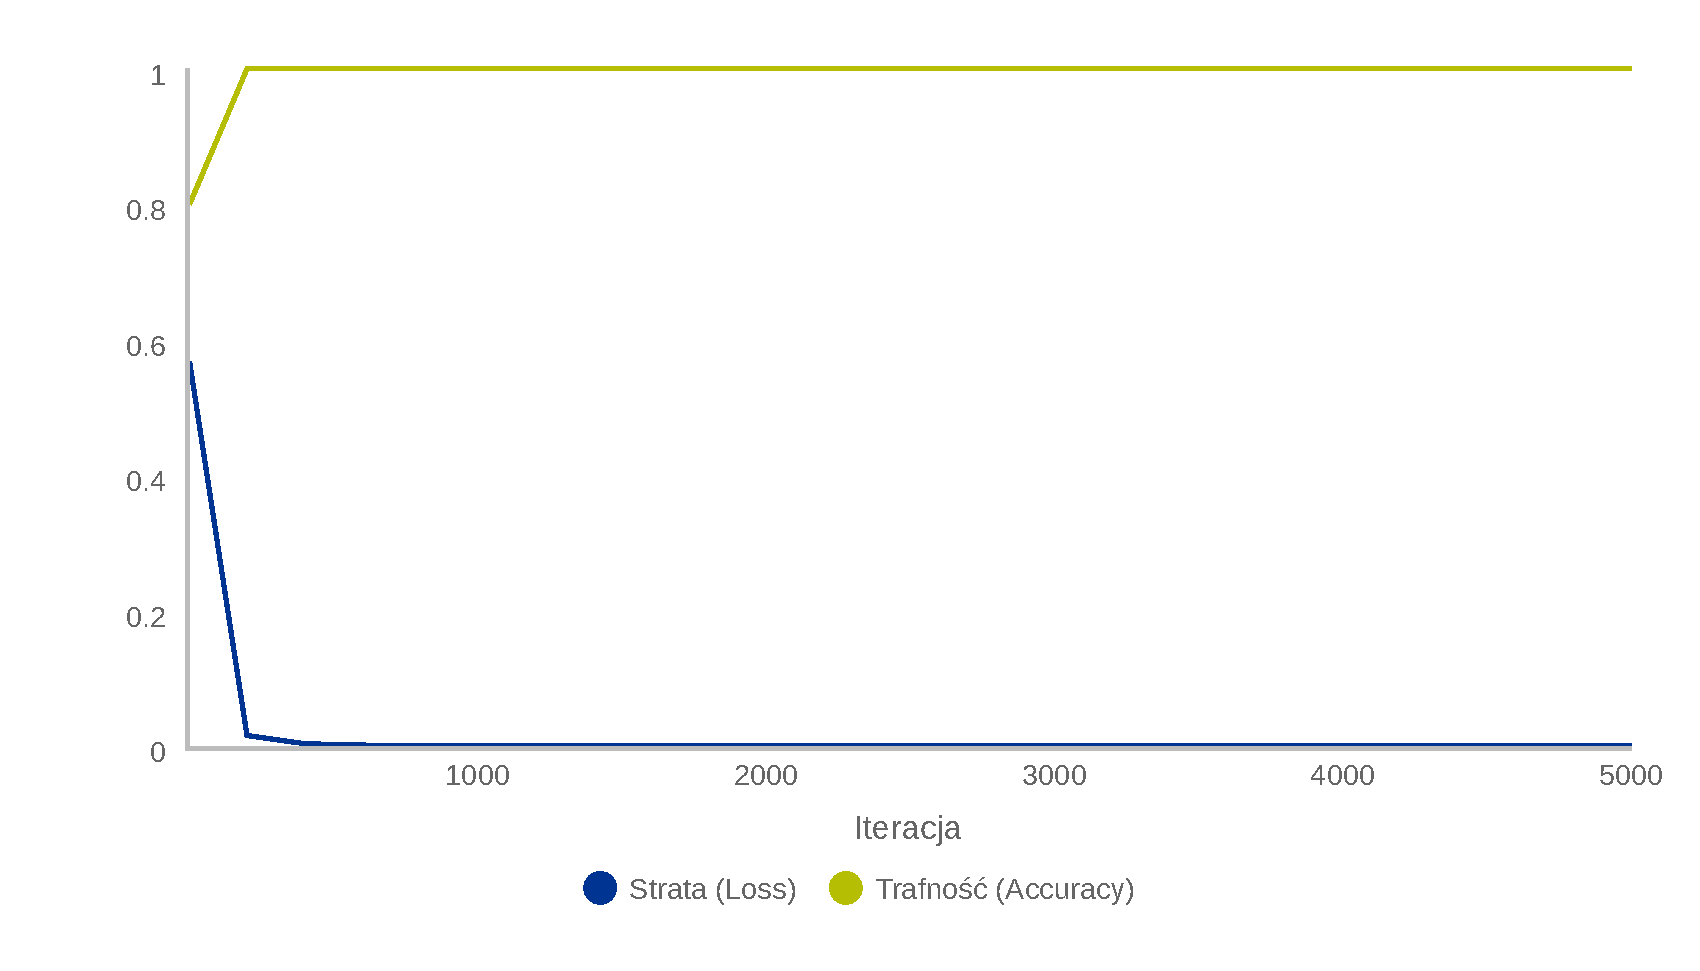
\includegraphics[width=0.53\textwidth]{learn/fake-ifs.eps}
\caption{Rezultat uczenia modelu bezwzględnego w~uproszczonej metryce jakości kodu traktującej negatywnie wyrażenia warunkowe}
\label{fig:learn:fake-ifs}
\end{wrapfigure}

Pierwszą -- trywialną -- metryką klasyfikującą zebrane metody było negatywne traktowanie wyrażenia warunkowego.

\begin{quotation}
\noindent Jeśli rozbiór syntaktyczny zawiera węzeł \texttt{IfStmt} lub \texttt{ConditionalExpr}, reprezentujący kolejno wyrażenie warunkowe \texttt{if} oraz warunkowy operator potrójny (z ang. \textit{ternary}) -- traktuj kod jako niskiej jakości. W~przeciwnym razie -- traktuj kod jako wysokiej jakości.
\end{quotation}

Według powyższej reguły 34526 metod zostało sklasyfikowane jako kod niskiej jakości (85\%).

Okazuje się, że~dla tak przygotowanych danych model potrzebuje tylko kilkadziesiąt iteracji uczenia by osiągnąć całkowitą skuteczność w~rozpoznawaniu przygotowanej definicji kodu niskiej jakości. Wynik ten nie był zaskakujący -- dla tak zdefiniowanego pojęcia jakości kodu wystarczy rzucić okiem na~implementację by wyznaczyć klasyfikację, którą powinien zwrócić model. Ten krok potwierdził jednak wstępnie poprawność implementacji modelu. Pełny przebieg uczenia zaprezentowano na~rysunku \ref{fig:learn:fake-ifs}.

\subsection{Wirtualna metryka bezwzględna}
\label{sec:learn:fake-static7}

\begin{wrapfigure}{R}{0.55\textwidth}
\centering
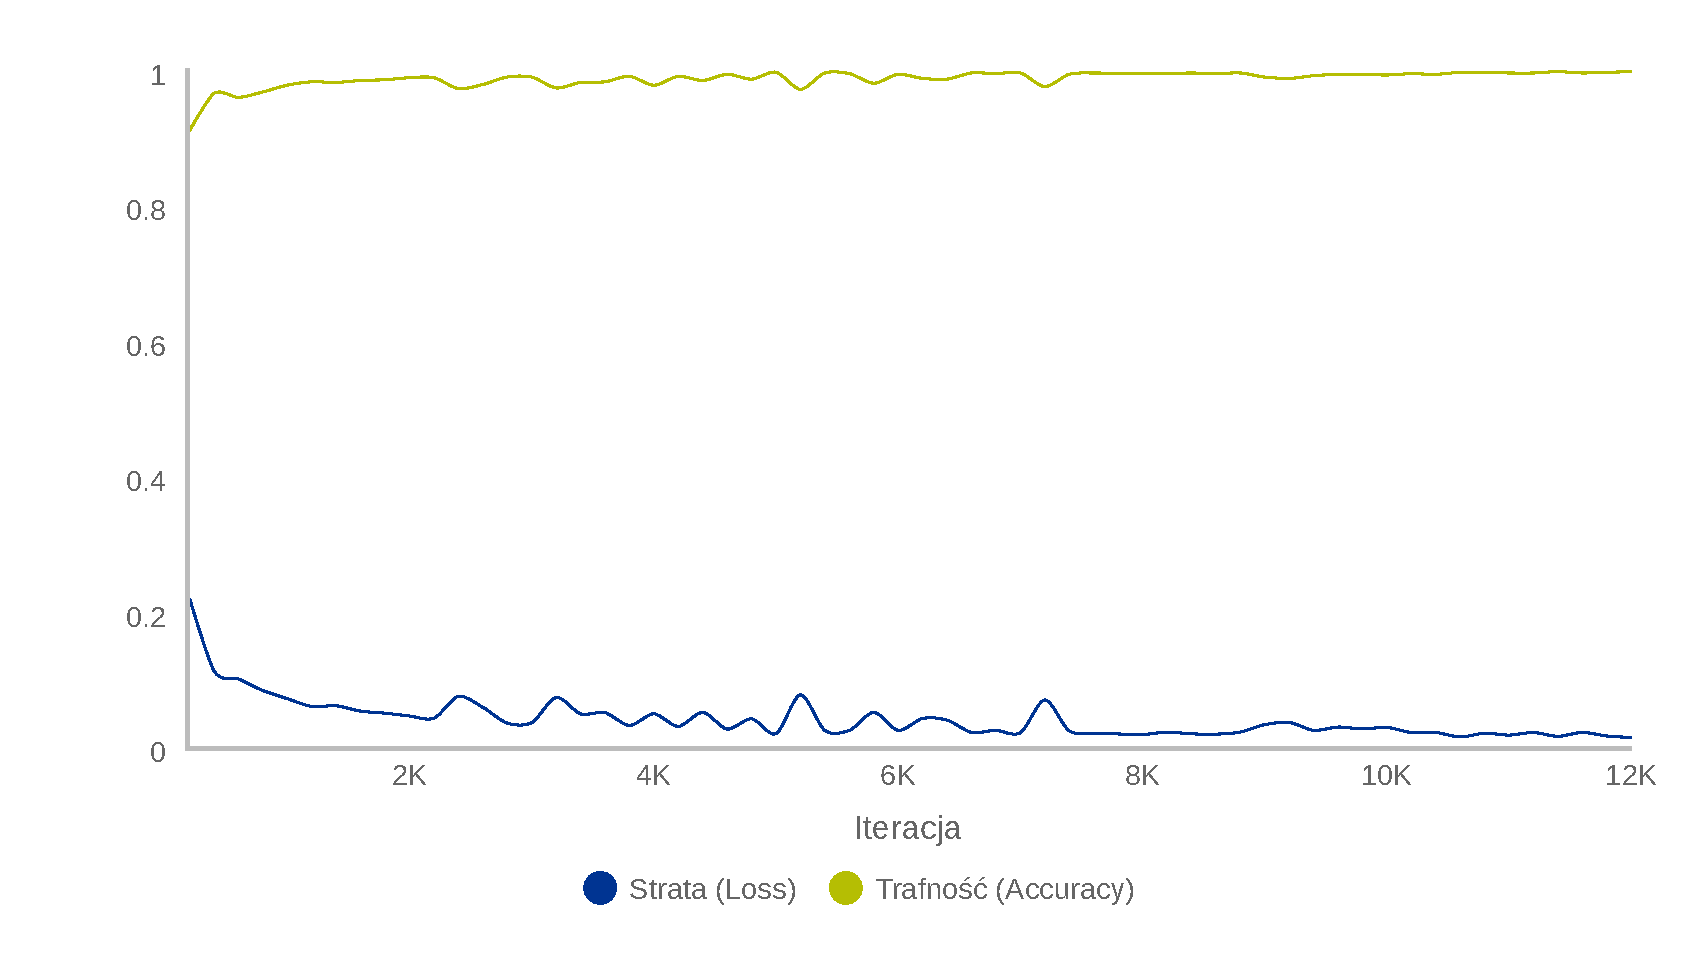
\includegraphics[width=0.53\textwidth]{learn/fake-static-7.eps}
\caption{Rezultat uczenia modelu bezwzględnego w~uproszczonej metryce jakości kodu zliczającej koszt wybranych konstrukcji językowych}
\label{fig:learn:fake-static7}
\end{wrapfigure}

Po uzyskaniu pozytywnego rezultatu przy zastosowaniu trywialnej metryki, podjęto próbę uczenia modelu klasyfikacją według bardziej złożonej reguły. W~tym celu przypisano wybranym konstrukcjom językowym stały koszt (rozumiany jako ,,koszt zrozumienia danej konstrukcji przez programistę'', idąc za~przykładem metryki Cognitive Complexity \cite{cognitive} wspomnianej w~sekcji \ref{sec:related:metrics}). Ustalone koszty poszczególnych konstrukcji językowych przedstawiono w~tabeli \ref{tbl:learn:fake-cost}. Metryka ta jest bardziej skomplikowana niż wariant pierwszy. Jeśli tak byłaby rozumiana jakość kodu źródłowego, programiście wystarczyłaby krótka analiza implementacji by stwierdzić czy jest ona czytelna. Model nie powinien mieć więc żadnych problemów z~rozpoznaniem nałożonych reguł.

\pagebreak

Druga metryka testowa jest zdefiniowana następująco.

\begin{quotation}
\noindent Jeśli koszt metody liczony według tabeli \ref{tbl:learn:fake-cost} przekroczy $7$, traktuj kod jako niskiej jakości. W~przeciwnym razie -- traktuj kod jako wysokiej jakości.
\end{quotation}

\begin{table}[h]
\centering
\caption{Koszt poszczególnych konstrukcji językowych w~przyjętej wirtualnej metryce kodu źródłowego}
\label{tbl:learn:fake-cost}
\begin{tabular}{|l|l|}
  \hline 
  \textbf{Typ węzła \gls{ast}} & \textbf{Koszt} \\ \hline
  \texttt{IntegerLiteralExpr} & 1 \\ \hline
  \texttt{StringLiteralExpr} & 1 \\ \hline
  \texttt{ConditionalExpr} & 2 \\ \hline
  \texttt{ForeachStmt} & 2 \\ \hline
  \texttt{IfStmt} & 2 \\ \hline
  \texttt{CastExpr} & 3 \\ \hline
  \texttt{ForStmt} & 3 \\ \hline
  \texttt{WhileStmt} & 3 \\ \hline
  \texttt{SwitchStmt} & 4 \\ \hline
\end{tabular} 
\end{table}

Wartość $7$ ustalono tak, aby reguła podzieliła posiadany zbiór danych w~stosunku 40\%:60\%. W~efekcie, 17181 metod (42\%) zostało sklasyfikowanych jako kod niskiej jakości.

Według tak przygotowanych danych, na~zbiorze testowym model wahał się bardziej niż przy pierwszej -- trywialnej -- metryce, ale i~tak po kilkudziesięciu iteracjach był w~stanie rozpoznać przygotowaną regułę klasyfikacji kodu i~jego trafność nie spadała poniżej 98\%. Przebieg uczenia zaprezentowano na~rysku \ref{fig:learn:fake-static7}.

\subsection{Wirtualna metryka zależna od długości metody}

Metryka zaproponowana w~sekcji \ref{sec:learn:fake-static7} nie traktowała sprawiedliwie dłuższych metod. Jeśli -- przykładowo -- metoda posiada 50 konstrukcji językowych, sprawiedliwa klasyfikacja powinna pozwolić jej na~osiągnięcie wyższego koszt niż metodzie, która zawiera ich tylko 20. Dlatego finalną metryką rozstrzygająca o~poprawnej implementacji modelu sieci neuronowej było uzależnienie kosztu, przy którym metoda była klasyfikowana jako niskiej jakości od jej długości. Poprawne wytrenowanie modelu dla takiej metryki przekonało już autora rozprawy, że problemów z~osiągnięciem pożądanej trafności jakościowego modelu należy szukać w~innym miejscu.

Ostatnią testową metrykę można zdefiniować w~następujący sposób.

\begin{quotation}
\noindent Jeśli stosunek kosztu metody liczonego według tabeli \ref{tbl:learn:fake-cost} do~długości metody wyrażonej w~liczbie węzłów \gls{ast} przekroczy $0.15$, traktuj kod jako niskiej jakości. W~przeciwnym razie -- traktuj kod jako wysokiej jakości.
\end{quotation}

\begin{wrapfigure}{R}{0.55\textwidth}
\centering
\includegraphics[width=0.53\textwidth]{learn/fake-static-15.eps}
\caption{Rezultat uczenia modelu bezwzględnego w~uproszczonej metryce jakości kodu zliczającej wybrane konstrukcje językowe i~klasyfikującej kod w~zależności od jego długości}
\label{fig:learn:fake-static15}
\end{wrapfigure}

Analogicznie do~poprzedniego przypadku -- wartość $0.15$ została ustalona empirycznie tak, by uzyskać zrównoważony podział danych wejściowych. Przy zastosowaniu tej reguły, 16533 metody (41\%) zostało sklasyfikowane jako kod niskiej jakości.

Również w~tym przypadku model poradził sobie z~odpowiednim klasyfikowaniem zbioru testowego. Przebieg uczenia przedstawiono na~rysunku \ref{fig:learn:fake-static15}. 

Na tym etapie zakończono testowanie zaimplementowanego modelu i~powrócono do~prób przekazania wiedzy do~modelu na~podstawie danych sklasyfikowanych według oryginalnych założeń.

\clearpage
\section{Opis implementacji mikrousługi udostępniającej klasyfikacje jakości kodu z~użyciem SCQM}
\label{apdx:scqm-docker}
\setcounter{table}{0}
\renewcommand{\thetable}{E.\arabic{table}}
\setcounter{figure}{0}
\renewcommand{\thefigure}{E.\arabic{figure}}
\setcounter{lstlisting}{0}
\renewcommand{\thelstlisting}{E.\arabic{lstlisting}}

Pierwotna postać implementacji modelu \gls{scqm}, która pozwoliła wytrenować go za~pomocą zgromadzonych danych została opisana w~dodatku \ref{apdx:scqm-impl}. Dla produkcyjnej wersji modelu głównym celem jest możliwość przyjęcia dowolnej próbki kodu źródłowego lub zmiany i~uzyskanie w~odpowiedzi prawdopodobieństw $P_G$ i~$P_B$, świadczących o~ich jakości.

Aby maksymalnie ukryć szczegóły implementacji, podjęto decyzję o~udostępnieniu interfejsu modelu w~postaci \gls{rest} \gls{api}. Jest to popularny sposób udostępniania funkcjonalności z~różnego rodzaju mikroserwisów -- i~właśnie tak autor rozprawy chciałby postrzegać wdrożeniową wersję modelu \gls{scqm}. Dzięki temu dowolny klient potrafiący wykonać żądanie \gls{http} będzie w~stanie sklasyfikować dowolny kod źródłowy.

\subsection{Mikrousługa wykonująca rozbiór syntaktyczny}

Zanim przystąpiono do~modyfikacji modelu w~języku Python, konieczne było dostarczenie implementacji parsera dla języka Java tak, by możliwe było przesyłanie w~zapytaniu kodu źródłowego bez żadnych przekształceń. To uruchomiona aplikacja \gls{scqm} powinna być odpowiedzialna za~odpowiednie przekształcenie kodu źródłowego i~przekazanie uzyskanej postaci wejścia dalej do~modelu w~TensorFlow.

Dotychczasowa implementacja parsera, opisana w~sekcji \ref{impl:ast:javaparser}, została wzbogacona o~\textit{framework} Spring Boot\footnote{\url{https://spring.io/projects/spring-boot}}, który umożliwia uruchomienie REST API w~aplikacjach opartych o~język Java. Z~aplikacji parsera udostępniany jest tylko jeden endpoint:

\begin{itemize}
    \item \texttt{POST /parse} -- umożliwia przesłanie kodu źródłowego klasy w~Javie; w~odpowiedzi klient uzyskuje listę metod odnalezionych w~klasie wraz z~ich ztokenizowanym rozbiorem syntaktycznym.
\end{itemize}

Każdy element tablicy będącej odpowiedzią parsera zawiera klucz \texttt{methodName} z~nazwą metody, \texttt{sourceCode} z~kodem źródłowym oraz \texttt{tokens} zawierający tablicę zawierającą elementy jego rozbioru syntaktycznego, zamienione na~liczbowe tokeny zgodnie z~opisiem metodyki przygotowania wejścia modelu w~sekcji \ref{sec:impl:rnn-input}.

Kod źródłowy parsera wraz z~\gls{rest} \gls{api} znajduje się w~repozytorium \cite{fracz:scqm} w~katalogu \path{java-parser}.

Listing \ref{lst:eval:parser:request} zawiera przykład poprawnego żądania do~parsera. Listing \ref{lst:eval:parser:response} zawiera odpowiedź na~to żądanie.

\begin{lstlisting}[frame=single,caption={Przykład poprawnego żądania do~REST API wystawionego przez aplikację z~parserem},captionpos=b,label={lst:eval:parser:request}]
POST http://localhost:8080/parse
{
  "source": "public class Dog {\n\tvoid bark() {\n\t\tSystem.out.println("Hau");\n\t}\n\n\tvoid sleep() {\n\t\tSystem.exit();\n\t}\n}\n"
}
\end{lstlisting}

\begin{lstlisting}[frame=single,caption={Przykład odpowiedzi z~REST API wystawionego przez aplikację z~parserem},captionpos=b,label={lst:eval:parser:response}]
[
  {
     "methodName": "sleep",
     "tokens": [74, 56, 74, 20, 74, 8, 74, 73, 4, 36, 4, 75, 75, 75, 74, 34, 75, 4, 75],
     "sourceCode": "void sleep() {\n    System.exit();\n}"
  },
  {
    "methodName": "bark",
    "tokens": [74, 56, 74, 20, 74, 8, 74, 73, 37, 4, 74, 48, 4, 36, 4, 75, 75, 75, 75, 74, 34, 75, 4, 75],
    "sourceCode":"void bark() {\n    System.out.println(\"Hau\");\n}"
  }
]
\end{lstlisting}

\subsection{Mikrousługa klasyfikująca kod za~pomocą modelu SCQM}

Jednym z~popularnych frameworków umożliwiających uruchomienie REST API w~dowolnej aplikacji pisanej w~języku Python jest Flask\footnote{\url{http://flask.pocoo.org}}. Ze~względu na~prostotę jego użycia, wdrożono go do~implementacji modelu \gls{scqm}.

Skrypt \path{scqm/scqm.py}\footnote{\url{https://github.com/fracz/scqm/blob/master/scqm-model/scqm.py}} w~repozytorium \cite{fracz:scqm} jest połączeniem implementacji \gls{ascqm} i~\gls{rscqm}, do~której dołożono także wsparcie \textit{frameworka} Flask i~wystawiono z~niego REST API umożliwiające przesłanie kodu źródłowego do~klasyfikacji. W~katalogu \path{trained/code-fracz-645}\footnote{\url{https://github.com/fracz/scqm/tree/master/trained/code-fracz-645}} znajdują się parametry wytrenowanego modelu dla najlepszej konfiguracji danych wejściowych i~parametrów uczenia opisanych w~rozdziale \ref{ch:learn}. W~trakcie uruchamiania skryptu modele odczytują te parametry, inicjalizując nimi zbudowany w~TensorFlow model. Jeśli to się uda, Flask uruchamia REST API, oferujące następujące punkty końcowe:

\begin{itemize}
    \item \texttt{GET /} -- udostępnia aplikację internetową zawierającą formularz do~przesyłania danych i~prezentacji odpowiedzi (zob. rysunki \ref{fig:eval:ascqm-form}, \ref{fig:eval:rscqm-form}, \ref{fig:eval:ascqm-result} i~\ref{fig:eval:rscqm-result})
    \item \texttt{POST /ascqm} -- umożliwia przesłanie kodu źródłowego jednej klasy; kod ten zostanie sklasyfikowany przy użyciu \gls{ascqm} i~w~odpowiedzi klient otrzyma klasyfikację przesłanego kodu oraz inne szczegółowe informacje (zob. listingi \ref{lst:eval:ascqm:request} i~\ref{lst:eval:ascqm:response})
    \item \texttt{POST /rscqm} -- umożliwia przesłanie kodu źródłówego dwóch klas, reprezentujących zmianę w~kodzie; zmiana ta zostanie sklasyfikowana przy użyciu \gls{rscqm} i~w~odpowiedzi klient otrzyma klasyfikację przesłanej zmiany oraz inne szczegółowe informacje (zob. listingi \ref{lst:eval:rscqm:request} i~\ref{lst:eval:rscqm:response})
\end{itemize}

Po otrzymaniu kodu źródłowego do~sklasyfikowania na~endpoincie \texttt{/ascqm} lub \texttt{/rscqm}, skrypt w~Pythonie odpytuje endpoint parsera w~celu otrzymania listy metod w~zadanej klasie oraz ich rozbioru syntaktycznego. Następnie, każda z~uzyskanych w~ten sposób sekwencji z~rozbiorem syntaktycznym jest dopełniana zerami tak, aby jej długość była równa maksymalnej długości sekwencji wejścia, która była ustalona w~trakcie uczenia. Zależy więc ona od parametrów wytrenowanego modelu, z~którym uruchomiono aplikację. Dłuższe metody na~tym etapie są odrzucane. Ponadto, w~przypadku wariantu względnego \gls{rscqm}, metody które istnieją zarówno w~kodzie klasy przed i~po zadanej zmianie są łączone w~pary, które stworzą wejście dla modelu. Metody, które zostały usunięte lub dodane w~ramach zmiany nie są uwzględniane w~modelu względnym (zob. ograniczenia modelu opisane w~sekcji \ref{sec:proj:constraints}).

Następnie, dla każdej rozpoznanej przez parser i~nieodrzuconej przez powyższe warunki metody lub pary w~zadanym kodzie źródłowym, odpowiedni model jest uruchamiany w~celu obliczenia wartości tensora \texttt{prediction} (zob. dodatek \ref{apdx:scqm-impl}). Dzięki temu dla każdej próbki uzyskiwane są wartości $P_G$ i~$P_B$ i~są zwracane w~odpowiedzi.

\subsection{Konfiguracja uruchomieniowa prototypu}
\label{sec:eval:docker}

Pomimo możliwości uruchomienia implementacji opisywanej mikrousługi na~dowolnym systemie operacyjnym, wymagałoby to od użytkownika instalacji i~konfiguracji odpowiednich wersji języków Python oraz Javy wraz ze~wszystkimi wymaganymi zależnościami. Dlatego podjęto decyzję o~dalszym uproszczeniu sposobu uruchomienia stworzonego modelu za~pomocą kontenerów Docker\footnote{\url{https://www.docker.com}}.

Konfiguracja kontenerów znajduje się w~katalogu \texttt{docker} w~repozytorium \cite{fracz:scqm}. Przygotowano dwa kontenery:

\begin{itemize}
    \item \texttt{scqm-parser}, zawierający środowisko aplikacji udostępniającej funkcjonalność parsera w~języku Java za~pomocą Spring Boot, oraz
    \item \texttt{scqm-model}, zawierający aplikację udostępniającą model \gls{scqm} za~pomocą \textit{frameworka} Flask.
\end{itemize}

Obydwa kontenery zostały połączone w~jedną aplikację za~pomocą Docker Compose\footnote{\url{https://docs.docker.com/compose/}}. Kontener z~parserem jest wykorzystywany tylko wewnątrz skryptu z~modelem, dlatego nie wystawiono dla niego żadnych portów sieciowych. Kontener z~modelem natomiast wystawia na~zewnątrz port 7276\footnote{nie jest to port przypadkowy; pisząc na~klawiaturze numerycznej telefonu ,,SCQM'' otrzymamy dokładnie wartość 7276}, pod którym dostępne jest REST API uruchomione przez \textit{framework} Flask.

\subsection{API}

Uruchomiona mikrousługa udostępnia REST API, które może być wykorzystane do~otrzymania klasyfikacji kodu źródłowego dowolnej klasy napisanej w~języku Java. W~tym celu udostępniono dwa punkty końcowe \texttt{/ascqm} oraz \texttt{/rscqm}, które pozwalają na~przesłanie odpowiednio jednej lub dwóch klas (zmiany) i~uzyskania ich klasyfikacji. Przykłady żądania i~odpowiedzi z~klasyfikacją kodu w~klasie dla modelu \gls{ascqm} przedstawiono na~listingach \ref{lst:eval:ascqm:request} i~\ref{lst:eval:ascqm:response}. Analogicznie, listingi \ref{lst:eval:rscqm:request} i~\ref{lst:eval:rscqm:response} przedstawiają żądanie i~odpowiedź dla modelu \gls{rscqm}.

\pagebreak

\begin{lstlisting}[frame=single,caption={Przykład poprawnego żądania do~REST API modelu aSCQM},captionpos=b,label={lst:eval:ascqm:request}]
POST http://localhost:7276/ascqm
{
  "source": "public class Dog {\n\tvoid bark() {\n\t\tSystem.out.println("Hau");\n\t}\n\n\tvoid sleep() {\n\t\tSystem.exit();\n\t}\n}\n"
}
\end{lstlisting}

\begin{lstlisting}[frame=single,caption={Przykład odpowiedzi z~predykcją dla modelu aSCQM},captionpos=b,label={lst:eval:ascqm:response}]
[
  {
    "methodName": "sleep", 
    "tokens": [74, 56, 74, 20, 74, 8, 74, 73, 4, 36, 4, 75, 75, 75, 74, 34, 75, 4, 75],
    "sourceCode": "void sleep() {\n    System.exit();\n}", 
    "prediction": [0.9346317648887634, 0.0653681755065918]
  }, 
  {
    "methodName": "bark", 
    "tokens": [74, 56, 74, 20, 74, 8, 74, 73, 37, 4, 74, 48, 4, 36, 4, 75, 75, 75, 75, 74, 34, 75, 4, 75],
    "sourceCode": "void bark() {\n    System.out.println(\"Hau\");\n}", 
    "prediction": [0.949866771697998, 0.05013318732380867]
  }
]
\end{lstlisting}

\begin{lstlisting}[frame=single,caption={Przykład poprawnego żądania do~REST API modelu rSCQM},captionpos=b,label={lst:eval:rscqm:request}]
POST http://localhost:7276/rscqm
{
  "sourceBefore": "public class Dog {\n\nvoid bark() {\nSystem.out.println(\"Hau\");\n}\n\nvoid sleep() {\nSystem.exit();}\n\n}",
  "sourceAfter": "public class Dog {\nprivate boolean sleeping = false;\nvoid bark() {\nif (!sleeping) {\n  System.out.println(\"Hau\");\n}\n}\n\nvoid sleep() {\nSystem.exit();}\n\n}"
}
\end{lstlisting}

% AST BEFORE
%{
%      "methodName": "sleep", 
%      "tokens": [74, 56, 74, 20, 74, 8, 74, 73, 4, 36, 4, 75, 75, 75, 74, 34, 75, 4, 75],
%      "sourceCode": "void sleep() {\n    System.exit();\n}"
%    },
%    {
%      "methodName": "bark", 
%      "tokens": [74, 56, 74, 20, 74, 8, 74, 73, 37, 4, 74, 48, 4, 36, 4, 75, 75, 75, 75, 74, 34, 75, 4, 75], 
%      "sourceCode": "void bark() {\n    System.out.println(\"Hau\");\n}"
%    }

% AST BEFORE
%{
%      "methodName": "sleep", 
%      "tokens": [74, 56, 74, 20, 74, 8, 74, 73, 4, 36, 4, 75, 75, 75, 74, 34, 75, 4, 75],
%      "sourceCode": "void sleep() {\n    System.exit();\n}"
%    },
%    {
%      "methodName": "bark", 
%      "tokens": [74, 56, 74, 20, 74, 66, 74, 26, 36, 4, 75, 74, 20, 74, 8, 74, 73, 37, 4, 74, 48, 4, 36, 4, 75, 75, 75, 75, 75, 75, 74, 34, 75, 4, 75], 
 %     "sourceCode": "void bark() {\n    if (!sleeping) {\n        System.out.println(\"Hau\");\n    }\n}"
  %  }

\pagebreak
\begin{lstlisting}[frame=single,caption={Przykład odpowiedzi z~predykcją dla modelu rSCQM},captionpos=b,label={lst:eval:rscqm:response}]
{
  "astBefore": [
    // Parser response for code "before"; skipped for clarity
  ], 
  "astAfter": [
     // Parser response for code "after"; skipped for clarity
  ], 
  "predictions": [
    {
      "methodName": "bark", 
      "methodBefore": {
        "methodName": "bark", 
        "tokens": [74, 56, 74, 20, 74, 8, 74, 73, 37, 4, 74, 48, 4, 36, 4, 75, 75, 75, 75, 74, 34, 75, 4, 75], 
        "sourceCode": "void bark() {\n    System.out.println(\"Hau\");\n}"
      }, 
      "methodAfter": {
        "methodName": "bark", 
        "tokens": [74, 56, 74, 20, 74, 66, 74, 26, 36, 4, 75, 74, 20, 74, 8, 74, 73, 37, 4, 74, 48, 4, 36, 4, 75, 75, 75, 75, 75, 75, 74, 34, 75, 4, 75],
        "sourceCode": "void bark() {\n    if (!sleeping) {\n        System.out.println(\"Hau\");\n    }\n}"
      }, 
      "prediction": [0.9768826961517334, 0.02311730943620205]
    }
  ]
}
\end{lstlisting}

Warto zwrócić uwagę, że~na listingach z~odpowiedziami \ref{lst:eval:ascqm:response} i~\ref{lst:eval:rscqm:response} są zawarte predykcje wyłącznie dla metod, które mogłybyć sklasyfikowane przez model (tj. nie były za~długie, a~w~przypadku \gls{rscqm} także istniały przed i~po zmianie). Odpowiedzi te generowane są bez zauważalnego opóźnienia (poniżej 500ms), więc predykcje te mogą być wykorzystywane w~rozwiązaniach, które wymagają szybkiej klasyfikacji kodu.

\subsection{Interfejs użytkownika}

Poza API, do~łatwego wykorzystania stworzonego modelu została dostarczona prosta aplikacja webowa, która umożliwia przesłanie kodu do~sklasyfikowania i~odczytania odpowiedzi w~przejrzystej dla użytkownika formie. 

Aplikacja wykorzystuje te same punkty końcowe, które zostały opisane powyżej. Jest ona dostępna po uruchomieniu modelu pod adresem \url{http://localhost:7276}. Do jej otwarcia wystarczy użyć dowolnej przeglądarki internetowej.

Rysunki \ref{fig:eval:rscqm-form} i~\ref{fig:eval:ascqm-form} przedstawiają formularze, do~których można wstawić kod źródłowy. Kolejne rysunki \ref{fig:eval:rscqm-result} i~\ref{fig:eval:ascqm-result} przedstawiają rezultaty takiej klasyfikacji po przesłaniu formularzy. Wartości $P_G$ i~$P_B$ podane dla całej klasy są średnią arytmetyczną tych samych wartości dla poszczególnych metod.

\begin{figure}[h!]
\centering
\includegraphics[width=\textwidth]{eval/rscqm-form.png}
\caption{Formularz pozwalający na~przesłanie kodu do~klasyfikacji przez model rSCQM}
\label{fig:eval:rscqm-form}
\end{figure}

\begin{figure}[h!]
\centering
\includegraphics[width=\textwidth]{eval/ascqm-form.png}
\caption{Formularz pozwalający na~przesłanie kodu do~klasyfikacji przez model aSCQM}
\label{fig:eval:ascqm-form}
\end{figure}

\begin{figure}[H]
\centering
\includegraphics[width=\textwidth]{eval/rscqm-result.png}
\caption{Rezultat klasyfikacji kodu klasy przez model rSCQM}
\label{fig:eval:rscqm-result}
\end{figure}

\begin{figure}[h!]
\centering
\includegraphics[width=\textwidth]{eval/ascqm-result.png}
\caption{Rezultat klasyfikacji kodu klasy przez model aSCQM}
\label{fig:eval:ascqm-result}
\end{figure}

\clearpage
\section{Instrukcja uruchomienia mikrousługi udostępniającej klasyfikacje jakości kodu z~użyciem SCQM}
\label{apdx:scqm-usage}
\label{sec:eval:scqm-usage}
\setcounter{table}{0}
\renewcommand{\thetable}{F.\arabic{table}}
\setcounter{figure}{0}
\renewcommand{\thefigure}{F.\arabic{figure}}
\setcounter{lstlisting}{0}
\renewcommand{\thelstlisting}{F.\arabic{lstlisting}}

Dzięki odpowiedniemu przygotowaniu aplikacji z~modelem \gls{scqm}, które zostało szczegółowo opisane w~dodatku \ref{apdx:scqm-docker}, do~jej uruchomienia wystarczy dowolny komputer z~zainstalowanym Dockerem. Wystarczy sklonować repozytorium z~aplikacją, przejść do~katalogu \texttt{docker} i~uruchomić aplikację za~pomocą narzędzia \texttt{docker-compose}. Lista komend, które należy wykonać, została przedstawiona na~listingu \ref{lst:eval:app:run}.

\begin{lstlisting}[frame=single,caption={Komendy uruchamiające aplikację z~modelem SCQM},captionpos=b,label={lst:eval:app:run}]
git clone https://github.com/fracz/scqm.git
cd scqm/docker
docker-compose up --build -d
\end{lstlisting}

Aby TensorFlow mógł zainicjalizować wszystkie struktury wytrenowanym modelem, wymagane jest posiadanie co najmniej 6GB pamięci operacyjnej. Warto też zwrócić uwagę, że~aplikacja może uruchamiać się nawet 10 minut. Aby zweryfikować, czy wszystkie operacje inicjalizacji zostały już wykonane, można sprawdzić logi kontenera \texttt{scqm-model}. Informacja o~działającej uruchomionej aplikacji od \textit{frameworka} Flask ostatecznie oznacza poprawne uruchomienie modelu i~gotowość na~przyjmowanie kodu źródłowego do~klasyfikacji (zob. listing \ref{lst:eval:app:logs}).

\begin{lstlisting}[frame=single,caption={Logi kontenera scqm-model informujące o~poprawnym uruchomieniu aplikacji},captionpos=b,label={lst:eval:app:logs}]
docker logs --tail=1 scqm-model
 * Running on http://0.0.0.0:5000/ (Press CTRL+C to quit)
\end{lstlisting}

Od tego momentu aplikacja jest dostępna pod adresem \url{http://localhost:7276}. Do otwarcia interfejsu użytkownika aplikacji udostępniającej model \gls{scqm} można użyć dowolnej przeglądarki internetowej.

\clearpage
\section{Przykładowa integracja SCQM i~systemu kontroli wersji}
\label{apdx:git-hook}
\setcounter{table}{0}
\renewcommand{\thetable}{G.\arabic{table}}
\setcounter{figure}{0}
\renewcommand{\thefigure}{G.\arabic{figure}}
\setcounter{lstlisting}{0}
\renewcommand{\thelstlisting}{G.\arabic{lstlisting}}

Na końcu niniejszego dodatku, na~listingu \ref{lst:pre-commit-hook} zaprezentowano przykładową implementację \textit{hooka} typu \texttt{pre-commit}, który przed stworzeniem nowej zmiany w~historii projektu odpytuje \gls{rest} \gls{api} mikrousługi \gls{scqm} (zob. sekcja \ref{sec:eval:scqm-usage}). Jeśli jakościowy model kodu źródłowego wykryje, że~\textit{commit} obniżałby jakość kodu źródłowego -- będzie on zablokowany z~odpowiednim komunikatem.

Przedstawione rozwiązanie na~początku swojego działania pozyskuje listę dodanych lub zmienionych w~danej zmianie plików. Nie ma sensu analizowanie kodu, który jest usuwany. Następnie sprawdzane jest, czy jest to kod napisany w~Javie -- poszukiwane jest po prostu rozszerzenie pliku \texttt{.java}. Dla każdego takiego pliku wykonywane jest żądanie \gls{http} do~uruchomionej aplikacji \gls{scqm}. W~zależności od sytuacji, wykonywane jest żądanie do~modelu

\begin{itemize}
    \item \gls{ascqm}, jeśli plik jest dodawany w~analizowanym \textit{commicie}, lub
    \item \gls{rscqm}, jeśli plik istniał już wcześniej i~analizowany \textit{commit} go modyfikuje.
\end{itemize}

Niezależnie od wybranego przypadku, dla każdego pliku w~odpowiedzi otrzymujemy liczby $P_G$ i~$P_B$ dla każdej odnalezionej w~nim metody spełniającej wymagania modelu, oznaczające prawdopodobieństwa że~dany kod lub dana zmiana jest odpowiedniej jakości. Skrypt wylicza na~ich podstawie średnią jakość kodu lub zmiany w~danymi pliku i~prezentuje programiście wartość $P_G*100$. Jest to procentowo wyrażona klasyfikacja kodu w~danym pliku jako odpowiedniej jakości. Jeśli którykolwiek z~plików nie spełnia zadanego warunku $P_G\geq0.5$, skrypt odrzuca tworzony \textit{commit}, zwracając programiście odpowiedni komunikat.

Oczywiście, programista zawsze ma możliwość pominięcia sprawdzenia przy wybranym \textit{commicie}, podając parametr \texttt{--no-verify} przy komendzie \texttt{git commit}. Pozwala ona na~wykonanie zmiany bez wyzwalania \textit{hooka} \texttt{pre-commit}, co całkowicie pomija sprawdzenie kodu za~jego pomocą. W~ten sposób można wykonać zmianę pomimo identyfikowania jej niskiej jakości, jeśli model dla danego przypadku będzie się mylić.

Listingi \ref{lst:eval:hook-good} i~\ref{lst:eval:hook-bad} zawierają przykładowe tworzenie nowego \textit{commita} w~repozytorium, w~którym wprowadzono integrację z~modelem \gls{scqm} za~pomocą opisanego \textit{hooka}. Pierwszy z~nich to przypadek gdzie \textit{commit} został utworzony, ponieważ nie naurszał nałożonych na~projekt reguł jakościowych. Drugi -- pokazuje jak wygląda komunikat dla programisty, gdy jakość kodu została sklasyfikowana jako zbyt niska.

\begin{lstlisting}[frame=single,caption={Próba wprowadzenia zmiany kodu odpowiedniej jakości wraz z~informacją pochodzącą z~hooka integrującego projekt z~SCQM},captionpos=b,label={lst:eval:hook-good}]
$ git \textit{commit} -am "Launching rockets working"
src/main/java/pl/edu/agh/rocket/MainLauncher.java: rSCQM: 100%
src/main/java/pl/edu/agh/rocket/LauncherHelper.java: rSCQM: 87%
src/test/java/pl/edu/agh/rocket/MainHelperTest.java: aSCQM: 95%

[rockets 3134794b6] Launching rockets working
 3 files changed, 35 insertions(+), 2 deletions(-)
 create mode 100644 src/test/java/pl/edu/agh/rocket/MainHelperTest.java
\end{lstlisting}

\begin{lstlisting}[frame=single,caption={Próba wprowadzenia zmiany kodu zbyt niskiej jakości zablokowanej przez hook integrujący projekt z~SCQM},captionpos=b,label={lst:eval:hook-bad}]
$ git \textit{commit} -am "Launching rockets working"
src/main/java/pl/edu/agh/rocket/MainLauncher.java: rSCQM: 100%
src/main/java/pl/edu/agh/rocket/LauncherHelper.java: rSCQM: 87%
src/test/java/pl/edu/agh/rocket/MainHelperTest.java: aSCQM: 5%

SCQM model detected that your \textit{commit} decreases the quality of the source code.
Pay attention to the files that has been marked with score lower than 50% and refactor your code.
\end{lstlisting}


W celu poprawnego działania \textit{hooka} wymagana jest instalacja języka PHP w~systemie operacyjnym (w tym języku właśnie został napisany przykładowy \textit{hook}). Skrypt należy umieścić w~katalogu projektu, w~którym powinna być wdrożona kontrola jakości za~pomocą stworzonego modelu, w~pliku \path{.git/hooks/pre-commit}.

Kod źródłowy skryptu jest dostępny także na platformie GitHub\footnote{\url{https://gist.github.com/fracz/a3d3a5e6d12a5538f2858a79fd568fd1}\\lub \url{https://github.com/fracz/phd/links/G.18}}.

\begin{lstlisting}[frame=single,caption={Przykładowy \textit{hook} \texttt{pre-commit} dla systemu kontroli wersji Git integrujący repozytorium z~modelem SCQM},captionpos=b,label={lst:pre-commit-hook}]
#!/usr/bin/env php
<?php

exec('git diff --cached --name-status | awk \'$1 != "D" { print $2 }\'', $changedFiles);

$allChangesWithGoodQuality = true;

foreach ($changedFiles as $changedFile) {
    if (!preg_match('#\.java$#i', $changedFile)) {
        continue;
    }
    $sourceCurrent = file_get_contents($changedFile);
    $sourceBefore = '';
    exec('git show HEAD:' . $changedFile . ' 2>&1', $sourceBefore, $exitCode);
    if ($exitCode === 0 && $sourceBefore) {
        $sourceBefore = implode(PHP_EOL, $sourceBefore);
        $rscqm = getScqm('rscqm', ['sourceBefore' => $sourceBefore, 'sourceAfter' => $sourceCurrent]);
        if ($rscqm) {
            $rscqmResult = array_column($rscqm['predictions'], 'prediction');
            $rscqmResult = array_column($rscqmResult, 0);
            $averageResult = array_sum($rscqmResult) / count($rscqmResult);
            $rscqmResult = round($averageResult * 100);
            echo sprintf("%s: rSCQM: %d%%\n", $changedFile, $rscqmResult);
            $allChangesWithGoodQuality &= $rscqmResult >= 50;
        }
    } else {
        $ascqm = getScqm('ascqm', ['source' => $sourceCurrent]);
        if ($ascqm) {
            $ascqmResult = array_column($ascqm, 'prediction');
            $ascqmResult = array_column($ascqmResult, 0);
            $averageResult = array_sum($ascqmResult) / count($ascqmResult);
            $ascqmResult = round($averageResult * 100);
            echo sprintf("%s: aSCQM: %d%%\n", $changedFile, $ascqmResult);
            $allChangesWithGoodQuality &= $ascqmResult >= 50;
        }
    }
}

if (!$allChangesWithGoodQuality) {
    echo PHP_EOL . 'SCQM model detected that your \textit{commit} decreases the quality of the source code.' . PHP_EOL;
    echo 'Pay attention to the files that has been marked with score lower than 50% and refactor your code.' . PHP_EOL;
    exit(1);
}

function getScqm($scqm, $data) {
    $dataString = json_encode($data);
    $ch = curl_init('http://localhost:7276/' . $scqm);
    curl_setopt($ch, CURLOPT_CUSTOMREQUEST, "POST");
    curl_setopt($ch, CURLOPT_POSTFIELDS, $dataString);
    curl_setopt($ch, CURLOPT_RETURNTRANSFER, true);
    curl_setopt($ch, CURLOPT_HTTPHEADER, [
        'Content-Type: application/json',
        'Content-Length: ' . strlen($dataString)
    ]);
    $result = curl_exec($ch);
    return json_decode($result, true);
}
\end{lstlisting}

%\chapter{Lista źródłowych repozytoriów dla ewaluacji rozwiązania}
%\label{apdx:eval_repo_list}

%Poniższa lista zawiera wszystkie repozytoria kodu źródłowego (68) pobrane z~portalu GitHub w~celu pozyskania danych do~ewaluacji przygotowanego modelu \gls{scqm}. Zgodnie z~opisem w~rozdziale \ref{ch:eval}, jest to lista najpopularniejszych 350 repozytoriów kodu źródłowego wygenerowana w~momencie rozpoczynania etapu ewaluacji rozwiązania i~zawiera tylko repozytoria, które nie pojawiły się na~liście w~Dodatku \ref{apdx:full_repo_list}.

%W celu przejrzenia kodu źródłowego repozytorium, należy użyć jego nazwy z~poniższej listy i~poprzedzić ją adresem URL portalu GitHub, np. \url{https://github.com/apache/incubator-dubbo}.

%Aby sprawdzić, jakie \textit{commity} refaktoryzacyjne zostały w~niej zidentyfikowane, należy przejść do~katalogu \path{results-evaluation} w~repozytorium \cite{fracz:refactor-extractor} i~odnaleźć tam katalog zawierający zmiany z~pobranego repozytorium. ze~względu na~fakt, że~znak \texttt{/} jest specjalnym znakiem w~systemie plików, przy tworzeniu nazw katalogów zamieniono go na~dwa myślniki \texttt{--}. Dlatego zmian wyciągniętych z~projektu \texttt{apache/incubator-dubbo} należy szukać w~katalogu \path{results-evaluation/apache/incubator--dubbo}\footnote{\url{https://github.com/fracz/refactor-extractor/tree/master/results-evaluation/apache--incubator-dubbo}}. 

%\begin{multicols}{2}
%\noindent {\small apache/incubator-dubbo\\proxyee-down-org/proxyee-down\\crossoverJie/JCSprout\\google/gson\\Snailclimb/JavaGuide\\jenkinsci/jenkins\\DrKLO/Telegram\\signalapp/Signal-Android\\react-community/lottie-react-native\\Konloch/bytecode-viewer\\eugenp/tutorials\\ctripcorp/apollo\\eclipse-vertx/vert.x\\arduino/Arduino\\TheAlgorithms/Java\\paolorotolo/AppIntro\\vondear/RxTool\\b3log/symphony\\apache/incubator-druid\\JeffLi1993/springboot-learning-example\\oracle/graal\\ityouknow/spring-boot-examples\\google/tink\\dbeaver/dbeaver\\react-native-community/react-native-camera\\alibaba/arthas\\xuxueli/xxl-job\\sharding-sphere/sharding-sphere\\apache/rocketmq\\QMUI/QMUI\_Android\\pagehelper/Mybatis-PageHelper\\material-components/material-compo\-nents-android\\cats-oss/android-gpuimage\\forezp/SpringCloudLearning\\LuckSiege/PictureSelector\\dyc87112/SpringBoot-Learning\\apache/incubator-skywalking\\android-hacker/VirtualXposed\\apache/flink\\GoogleContainerTools/jib\\asLody/VirtualApp\\Justson/AgentWeb\\JessYanCoding/AndroidAutoSize\\Blankj/awesome-java-leetcode\\gyf-dev/ImmersionBar\\firebase/quickstart-android\\hs-web/hsweb-framework\\vipshop/vjtools\\yanzhenjie/AndPermission\\smuyyh/BookReader\\TooTallNate/Java-WebSocket\\guardianproject/haven\\TeamNewPipe/NewPipe\\pardom-zz/ActiveAndroid\\MindorksOpenSource/android-interview-questions\\sqshq/PiggyMetrics\\janishar/mit-deep-learning-book-pdf\\elasticjob/elastic-job-lite\\Activiti/Activiti\\NLPchina/elasticsearch-sql\\lets-blade/blade\\gzu-liyujiang/AndroidPicker\\alibaba/UltraViewPager\\barteksc/AndroidPdfViewer\\careercup/CtCI-6th-Edition\\checkstyle/checkstyle\\google/cameraview\\uber/RIBs}
%\end{multicols}

\clearpage
\section{Biografia naukowa doktoranta}
\setcounter{table}{0}
\renewcommand{\thetable}{H.\arabic{table}}
\setcounter{figure}{0}
\renewcommand{\thefigure}{H.\arabic{figure}}
\setcounter{lstlisting}{0}
\renewcommand{\thelstlisting}{H.\arabic{lstlisting}}

\paragraph{Dane bibliometryczne}
\begin{itemize}
    \item h-index: 1
    \item Wykaz publikacji BPP AGH \\\url{https://bpp.agh.edu.pl/autor/fracz-wojciech-20298}
    \item ORCiD \\\url{https://orcid.org/0000-0002-3613-6335}
    \item ResearchGate \\\url{https://www.researchgate.net/profile/Wojciech_Fracz}
    \item StackOverflow \\\url{https://stackoverflow.com/users/878514/fracz}
\end{itemize}

\paragraph{Tytuły naukowe}
\begin{itemize}
\item inż., 2013, temat pracy: \textit{System zamawiania posiłków wykorzystujący możliwości urządzeń mobilnych oraz mechanizmy lokalizacji użytkownika}, promotor: dr inż. Robert Marcjan
\item mgr inż., 2014, temat pracy: \textit{Wspieranie praktyki przeglądu kodu
źródłowego na~urządzeniach mobilnych}, promotor: dr inż. Jacek Dajda, praca dyplomowa obroniona z~wyróżnieniem
\end{itemize}

\paragraph{Publikacje}
\begin{itemize}
\item W. Frącz, J. Dajda. (2018). \textit{Developers' Game: a~Preliminary Study Concerning a~Tool for Automated Developers Assessment}. 2018 IEEE International Conference on Software Maintenance and Evolution (ICSME). IEEE, 2018. p. 695-699.
\\MNiSW=15

\item M. Piech, W. Frącz, W. Turek, M. Kisiel-Dorohinicki, J. Dajda, A. Byrski. (2018). \textit{Model for Dynamic and Hierarchical Data Repository in Relational Database}. Computer Science ; ISSN 1508-2806. — 2018 vol. 19 no. 4, s. 479–500.
\\MNiSW=12

\item W. Frącz, J. Dajda. (2017). \textit{Experimental Validation of Source Code Reviews on Mobile Devices}. International Conference on Computational Science and Its Applications (pp. 533-547). Springer, Cham.
\\MNiSW=15

\item W. Frącz, J. Dajda. (2016). \textit{Source code reviews on mobile devices}. Computer Science ; ISSN 1508-2806. — 2016 vol. 17 no. 2, s. 143–161.
\\MNiSW=12

\item W. Frącz. (2015). \textit{An empirical study inspecting the benefits of gamification applied to university classes}. 7th Computer Science and Electronic Engineering Conference (CEEC) (pp. 135-139). IEEE.
\\MNiSW=15

\item W. Frącz, J. Dajda. (2014) \textit{Can the source code be reviewed on a~smartphone?}. Software engineering from research and practice perspectives / eds. Lech Madeyski, Mirosław Ochodek. — Poznan; Warszawa: Wydawnictwo Nakom, 2014. — ISBN: 978-83-63919-16-0. — S. 179–195.
\\MNiSW=5

\end{itemize}

\paragraph{Nagrody i~wyróżnienia}
\begin{itemize}
\item Wyróżnienie Rektora AGH zespołowe III stopnia za~osiągnięcia dydaktyczne, zaprojektowanie i~przeprowadzenie bloku zajęć z~użyciem grywalizacji, wspólnie z~dr~inż.~Jackiem Dajda, 2017
\end{itemize}

\paragraph{Udział w~projektach badawczo-rozwojowych}
\begin{itemize}
\item \textit{Centrum Mistrzostwa Informatycznego}, Akademia Górniczo – Hutnicza im. Stanisława Staszica w~Krakowie, nr projektu POPC.03.02.00-00-0002/18, kierownik: dr hab. inż. Aleksander Byrski, prof. AGH, 2019

\item \textit{Wykorzystanie danych gromadzonych w~repozytoriach kodu źródłowego w~celu poprawy jakości pracy programistów i~popularyzacji przeglądów kodu źródłowego}, Akademia Górniczo-Hutnicza im. Stanisława Staszica w~Krakowie, grant dziekański (umowa nr 15.11.230.399), kierownik: dr hab. inż. Marek Kisiel-Do\-ro\-hi\-ni\-cki, prof. AGH, 2018

\item \textit{Wsparcie praktyki przeglądu kodu źródłowego na~urządzeniach mobilnych}, Akademia Górniczo-Hutnicza im. Stanisława Staszica w~Krakowie, grant dziekański (umowa nr 15.11.230.289), kierownik: dr hab. inż. Marek Kisiel-Dorohinicki, prof. AGH, 2016-2017

\item \textit{Europejskie dziedzictwo techniczne - upowszechnienie historycznych i~współczesnych publikacji z~zakresu nauk technicznych w~innowacyjnym środowisku informatycznym.}, Programu Operacyjnego Polska Cyfrowa, Europejskiego Funduszu Rozwoju Regionalnego, kierownik: dr hab. inż. Aleksander Byrski, prof. AGH, 2016-2019

\item \textit{Zastosowanie technik gamifikacji w~inżynierii oprogramowania}, Akademia Gó\-rni\-czo-Hutnicza im. Stanisława Staszica w~Krakowie, grant dziekański (umowa nr 15.11.230.192), kierownik: dr hab. inż. Marek Kisiel-Dorohinicki, prof. AGH, 2015

\item \textit{System gromadzenia i~generowania informacji na~potrzeby analizy kryminalnej i~koordynacji działań w~Straży Granicznej}, Narodowe Centrum Badań i~Rozwoju, kierownik: dr hab. inż. Marek Kisiel-Dorohinicki, prof. AGH, 2014-2017

\item \textit{System zarządzania informacjami w~transmisji elektronicznej (radio, TV)}, Narodowe Centrum Badań i~Rozwoju, kierownik: dr hab. inż. Marek Kisiel-Do\-ro\-hi\-ni\-cki, prof. AGH, 2014-2017

\item \textit{Opracowanie systemu koordynacji kontroli ,,PORTY 24''}, Izba Celna w~Gdyni, kierownik: dr inż. Jacek Dajda, 2014-2015

\item \textit{DiSSBy Systemy informacyjno-analityczny wspomagający planowanie działań BOR}, Ministerstwo Nauki i~Szkolnictwa Wyższego, kierownik: dr hab. inż. Marek Kisiel-Dorohinicki, prof. AGH, 2013-2016

\end{itemize}

\paragraph{Staże}
\begin{itemize}
\item Staż asystencki, Akademia Górniczo-Hutnicza im. Stanisława Staszica w~Krakowie, Wydział Informatyki, Elektroniki i~Telekomunikacji, Katedra Informatyki, Październik 2013 -- Wrzesień 2014.
\end{itemize}


\paragraph{Aktywność jako recenzent}
\begin{itemize}
\item Computing and Informatics, Institute of Informatics Slovak Academy of Sciences, 2018
\item International Conference on Computational Science and Its Applications, 2017
\item Computer Science, Akademia Górniczo-Hutnicza im. Stanisława Staszica w~Krakowie, 2016
\end{itemize}


\paragraph{Udział w~konferencjach}
\begin{itemize}
\item 34th 2018 IEEE International Conference on Software Maintenance and Evolution (ICSME), 26-28 września 2018, Madryt, Hiszpania
\item 17th International Conference on Computational Science and Its Applications (ICCSA 2017), 3-6 lipca 2017, Trieste, Włochy
\item 7th Computer Science and Electronic Engineering Conference (CEEC), 24-25 września 2015, Colchester, Wielka Brytania
\end{itemize}


\paragraph{Działalność dydaktyczna}
\begin{itemize}
\item Tworzenie nowoczesnych aplikacji internetowych, 1. rok studiów stac. W~ramach programu Prymusi AGH, 2018-2019
\item Podstawy programowania w~Javie, 1. rok studiów stac. W~ramach programu Prymusi AGH, 2018
\item Introduction to web programming, studenci z~uczelni EFREI w~Paryżu, 2018-2019
\item Java 1, studenci z~uczelni EFREI w~Paryżu, 2018
\item Programowanie aplikacji webowych 2, studia podyplomowe: Metody Wytwarzania Oprogramowania, 2018-2019
\item Prelekcja \textit{SUPLA -- otwarta, polska automatyka budynkowa} w~ramach Nocy Informatyka 1.1, 2018, \url{https://www.youtube.com/watch?v=5WobKP58YIk}
\item Techniki obiektowe i~komponentowe, studia podyplomowe: Projektowanie, Programowanie i~Eksploatacja Systemów, 2017-2019
\item Techniki programowania w~Javie 3, wykład \textit{Wprowadzenie do Javy}, studia podyplomowe: Metody Wytwarzania Oprogramowania, 2017-2019
\item Prelekcja \textit{Nowoczesny stos JS w~60 minut} w~ramach cyklu spotkań \textit{Epizody} (s17e02) organizowanego przez Koło Naukowe Epicentrum (UJ), 2017, \\\url{https://www.youtube.com/watch?v=nrCejJjxMe4}
\item Inżynieria oprogramowania, 3. rok studiów stac. I~stopnia na~kierunku Informatyka, 2015-2019
\item Wykład \textit{Git demystified}, 2015, 2019
\item Techniki wytwarzania oprogramowania, 2. rok studiów stac. II stopnia na~kierunku Informatyka, 2014-2017
\item Technologie obiektowe 2, 3. rok studiów stac. I~stopnia na~kierunku Informatyka, 2014-2018
\item Technologie obiektowe 1, 2. rok studiów stac. I~stopnia na~kierunku Informatyka, 2014-2018
\end{itemize}

\paragraph{Umiejętności}

\begin{itemize}
\item języki obce: angielski
\item języki programowania: Java, PHP, JavaScript
\item frameworki webowe (frontend): AngularJS, Vue.js, Aurelia, Bootstrap
\item frameworki webowe (backend): Symfony, Slim, Spring
\item zarządzanie projektami: Git, Maven, Gradle, Composer, NPM, JSPM, Webpack, Gulp
\end{itemize}

%\bibliography{bibliography}
%\bibliographystyle{unsrt}

\end{document}
